% The theory paper of Paper VI of the hemigroup programme (slug `pyramids`, module `pyramids`,
% tag v0.1; adr/0007): blueprint chapters 2-5. Its supplement (supplement.tex) prints Appendix A
% of the blueprint, the discrete stratum on the line. The computation paper is ../paper-b/.
%
% One file per section; every statement shared with the blueprint stands under a
% `% shared with blueprint <label>` marker, with the paper's \label equal to the blueprint's, so
% that `linkage check` reports it `verbatim`. Statements are transcribed from the blueprint, never
% from draft/. Section 1.1 owns the trust base.
%
% The paper and the supplement refer to each other through xr-hyper, so each is built after the
% other: latexmk -pdf main.tex supplement.tex, then once more (README.md). The \date line is the
% one `linkage release` reads; supplement.tex has a copy of it.
%
% Voice and register: article-kit docs/WRITING.md. LaTeX is written with the file tools, never
% through shell heredocs.
\documentclass[11pt]{article}
\newcommand{\pyrexternal}{supplement}
% The preamble of the two roots of the theory paper (main.tex, supplement.tex), on the model of
% the isotropic paper's (spatial-hemigroup-affine, paper-iso/preamble.tex). A root that defines
% \pyrexternal as the name of the other document reads that document's labels through xr-hyper,
% which is loaded before hyperref; the option nocite keeps the other document's bibliography
% numbers out, so that each has its own list of references.
\usepackage[a4paper,margin=1in]{geometry}
\setlength{\emergencystretch}{1.5em}
\usepackage{amsmath,amssymb,amsthm}
\usepackage{booktabs}
\usepackage{array}
\usepackage{longtable}
\newcolumntype{R}[1]{>{\raggedright\arraybackslash}p{#1}}
\newcolumntype{S}[1]{>{\footnotesize\raggedright\arraybackslash}p{#1}}
\setlength{\LTcapwidth}{\textwidth}
\usepackage{graphicx}
\usepackage{tikz}
% The figures are drawn by scripts/make_figures_theory.py into figures/ (theory-*.png).
\graphicspath{{../figures/}}
% natbib in numeric mode, for \citenum: the blueprint writes a citation with its locator as
% [\sscite{key}, Thm.~x, p.~y], so \sscite prints the bare number (macros.tex).
\usepackage[numbers]{natbib}
\ifdefined\pyrexternal\usepackage{xr-hyper}\fi
\usepackage[hidelinks]{hyperref}
\hypersetup{
  pdftitle={Spatial Scale Space from Hemigroup Axioms: The Theory of Image Pyramids},
  pdfauthor={Daniel Fagerstr\"om},
}

% The macros of the theory paper and its supplement. The blueprint's (blueprint/src/macros.tex)
% are kept by name, so that a statement shared with the blueprint compiles here unchanged and
% `linkage check` compares the same source text; three of them print differently here:
%   \prog{<module> v0.1}{<number>}  a citation of the released module, by its printed number;
%   \ledger{A<n>}                   the cited fact's own statement in section 2.2, by number;
%   \sscite{<key>}                  \cite.
% The leanblueprint metadata (\lean, \uses, \leanok, \notready) is not transcribed; the commands
% are defined empty so that a statement copied with them would still build.

\newcommand{\RR}{\mathbb{R}}
\newcommand{\CC}{\mathbb{C}}
\newcommand{\NN}{\mathbb{N}}
\newcommand{\ZZ}{\mathbb{Z}}
\newcommand{\Cin}{\operatorname{Cin}}   % the entire cosine integral, as in the cone module
\newcommand{\Levy}{L\'evy}              % the name, accented through one macro
\newcommand{\Matern}{Mat\'ern}          % the same device for the Matern family
\newcommand{\Polya}{P\'olya}            % and for Polya frequency functions
\newcommand{\GL}{\mathrm{GL}}
\newcommand{\Orth}{\mathrm{O}}          % the orthogonal group O(d)
\newcommand{\tp}{\mathsf{T}}            % transpose, written A^{\tp}
\newcommand{\tr}{\operatorname{tr}}
\newcommand{\diag}{\operatorname{diag}}
\newcommand{\PD}{\mathrm{PD}}           % positive definite d x d matrices
\newcommand{\Id}{\mathrm{Id}}
\newcommand{\Geom}{\mathrm{Geom}}       % the geometric law

\providecommand{\lean}[1]{}
\providecommand{\leanok}{}
\providecommand{\uses}[1]{}
\providecommand{\notready}{}
\providecommand{\proves}[1]{}
\providecommand{\notes}[1]{}
\providecommand{\statedin}[1]{}
\providecommand{\restates}[1]{}

% The blueprint writes every citation as [\sscite{key}] or [\sscite{key}, <locator>], so \sscite
% prints the bare number and the brackets are the text's.
\newcommand{\sscite}[1]{\citenum{#1}}

% The released modules of the programme, by the first argument of \prog as the blueprint writes
% it; the citekeys are the library's (hub constellation.json; paper/references.bib).
\makeatletter
\@namedef{progkey@V-line v0.1}{fagerstrom2026spatial}
\@namedef{progkey@V-cone v0.1}{fagerstrom2026cone}
\@namedef{progkey@V-selection v0.1}{fagerstrom2026selection}
\@namedef{progkey@iso v0.1}{fagerstrom2026isotropic}
\@namedef{progkey@affine v0.1}{fagerstrom2026affine}
\newcommand{\prog@key}[1]{\@ifundefined{progkey@#1}{\PackageError{macros}{No citation for the
  programme label #1}{}}{}\edef\prog@thekey{\csname progkey@#1\endcsname}}
\newcommand{\prog@cite}[2]{\cite[#2]{#1}}
\DeclareRobustCommand{\prog}[2]{\prog@key{#1}\expandafter\prog@cite\expandafter{\prog@thekey}{#2}}
\DeclareRobustCommand{\progpaper}[1]{\prog@key{#1}\expandafter\cite\expandafter{\prog@thekey}}
\makeatother

% A ledger entry is printed as its statement in section 2.2 (the node thm:cited-A<n>). The \ref is
% reached through \csname so that `linkage paper`, which reads \ref{...} arguments as labels, does
% not take the macro parameter for one.
\newcommand{\ledger}[1]{Theorem~\csname ref\endcsname{thm:cited-#1}}

% The other document is imported after macros.tex: its .aux carries titles written in the
% paper's macros (\Levy), which xr expands as it reads them.
\ifdefined\pyrexternal\externaldocument[][nocite]{\pyrexternal}\fi
\numberwithin{equation}{section}

% The blueprint numbers its four statement environments on one counter; so does the paper.
\theoremstyle{plain}
\newtheorem{theorem}{Theorem}[section]
\newtheorem{proposition}[theorem]{Proposition}
\newtheorem{lemma}[theorem]{Lemma}
\newtheorem{corollary}[theorem]{Corollary}
\theoremstyle{definition}
\newtheorem{definition}[theorem]{Definition}
\newtheorem{example}[theorem]{Example}
\theoremstyle{remark}
\newtheorem{remark}[theorem]{Remark}


\title{Spatial scale space from hemigroup axioms:\\
the theory of image pyramids}
\author{Daniel Fagerstr\"om}
% The release pyramids-v0.1 (records/pyramids/RELEASE-prep-pyramids-v0.1.md): the date, the version
% and the version DOI. The draft line, restored at the first edit after the release:
% \date{Working draft --- not yet released}
\date{November 23, 2026 (v0.1)\\[3pt] {\normalsize \href{https://doi.org/10.5281/zenodo.24480183}{doi:10.5281/zenodo.24480183}}}

\begin{document}
\maketitle

% The abstract: compared with the statements it summarizes before any freeze (the rule that
% summaries drop hypotheses).
\begin{abstract}
An image pyramid smooths and subsamples an image by a fixed ratio $q$ at every level. The classical
design literature constrains the kernel of one step and follows the equivalent kernels that the
pyramid builds level by level. Scale-space theory has a kernel at every scale and leaves the
subsampling outside its treatment. This paper studies kernel
families on $\RR^d$ under the hemigroup axioms of linear scale space, in which two consecutive
smoothing steps compose to one, with covariance under the powers of $q$ in place of every dilation.
It gives a description of the families by their \Levy{} data, a selection theorem and an
obstruction on the grid. The isotropic
families form three nested strata: all of them, those covariant under the powers of $q$, and those
covariant under every dilation. In the middle stratum the kernel from the scale $0$ to each scale
is semi-selfdecomposable: it is its own contraction by $q$, smoothed by an infinitely divisible law.
The scales are labelled so that
dilating the kernel at a scale $t$ by $q$ gives the kernel at $qt$, and an octave step goes from $t$ to $qt$. The ladder of octave steps between the stored levels determines the kernels at
the knots $q^n$. No law of bounded support other than a point mass is a step of any family that obeys
the cascade and is continuous in scale. Every octave step of the \Matern{} pyramid is one implicit
heat step, a Helmholtz resolvent, and the pyramid is covariant under every dilation. Up to a
relabelling $g$ of the scales with $g(qt) = q\,g(t)$, it is
the one isotropic family covariant under $q$ whose octave steps from every scale obey the maximum
principle of an implicit Euler step for every smooth rapidly decreasing input. Among symmetric
rotation-invariant laws the principle holds exactly for the Helmholtz resolvents, so Gaussian steps
fail it. The principle is required of the octave steps only. A step of the \Matern{} pyramid has it
only across a factor $q$ in scale, and no symmetric family has it at every step. A grid pyramid
applies one mask, a probability law, at every level, and it is called exact when the steps it
applies from level to level are the octave steps of one family continuous in scale and covariant
under $q$. On a lattice, a symmetric probability mask other than a point mass has an exact grid
pyramid if and only if it is infinitely divisible with a logarithmic moment. For laws the
sufficiency is a theorem of Maejima and Ueda, and continuity in scale gives the necessity. For an
integer ratio the kernels of an exact grid pyramid on $h\ZZ^d$ are singular. In
$d \ge 2$ no kernel at a positive scale of an exact grid pyramid whose mask is carried by a lattice
is rotation invariant. The same holds when the dilation is an invertible matrix, which may also turn
the lattice. The obstruction needs continuity in scale: some band-limited mask $w$ of infinite
support has a rotation-invariant law $\mu$ with $D_q\mu = \mu * w$. The lemmas, propositions and
theorems of Sections 3 to 6 and of the supplement have formal counterparts in Lean~4. All are machine-checked but one step and three
results proved in print only, in whole or in part: the proposition on matrix dilations, the
singularity clause on the kernels, and the band-limited example. The formal counterparts rest on
nine cited facts, taken as fourteen axioms that the supplement prints in Lean, and on two earlier
formal developments of the author's. One of the nine is a proposition of an earlier paper of the
author's that restates a theorem of Karlin. Neither the connecting prose nor the
numerical examples are machine-checked, and the formal statements and definitions were compared
with the printed ones by AI agents only.
\end{abstract}


% Section 1 of the theory paper (adr/0007): the introduction, written for the theory alone, and
% section 1.1, which owns the trust base (article-kit WRITING.md section 4). Statement numbers are
% \ref'd, never typed; the computation paper is unreleased and is named only as further work.
\section{Introduction}
\label{sec:intro}

An image pyramid stores an image at a sequence of resolutions. Each level is a smoothed copy of the
one before, subsampled by a fixed ratio $q$, usually $2$ \cite{burt1981fast,burt1983laplacian}. The
design literature constrains the generating kernel of one step. Burt and Adelson require it to be
separable, normalized, symmetric and of equal contribution \cite[p.~533]{burt1983laplacian}. Meer,
Baugher and Rosenfeld judge it by its distance from the ideal low-pass filter for decimation by $2$,
measured by the share of the spectrum folded back and by the error in the passband
\cite[pp.~513--515]{meer1987frequency}. Burt
observed that the equivalent kernels of the levels approach one shape \cite{burt1981fast}. What the
literature does not state is a property of the whole family of kernels: every level looks like every
other on its own grid. As an axiom, this is covariance under the dilations by $q^n$, $n \in \ZZ$,
which leaves every other dilation optional.

Scale-space theory supplies the rest. Its classical axioms require a semigroup of linear smoothings,
$\Phi_{t+s} = \Phi_t\Phi_s$ \cite[\S 3, Axiom~6, p.~270]{duits2004axioms},
\cite[\S 2.4.4, p.~41]{lindeberg1994scale}, as in Lindeberg's scale space for discrete signals
\cite{lindeberg1990scalespace}. Iijima's axioms, the earliest, require less: two smoothings compose to
a third, of some scale \cite[\S 3, p.~241]{weickert1999linear}.
Lindeberg notes that this theory does not cover pyramids, with their shrinking grids and fixed
sampling of scale. He asks how far a subsampling can enter a scale-space representation and keep the
properties that come from a continuous scale parameter \cite[\S 3.4.1, p.~82; \S 4.5.4,
p.~122]{lindeberg1994scale}.
The author's earlier papers replace the semigroup by a \emph{hemigroup}: a family of operators
$\Phi_{s,t}$ from scale $s$ to scale $t$ in which two consecutive steps compose to one,
$\Phi_{t,u}\Phi_{s,t} = \Phi_{s,u}$. This cascade ties the scale to no additive parameter. With
continuity in scale, symmetry, positivity and covariance under every dilation, the hemigroup axioms
classify the families of kernels on the line \prog{V-line v0.1}{Thm.~7.3, p.~37}, and in $\RR^d$ the
isotropic ones \prog{iso v0.1}{Thm.~3.6, p.~13}. Covariance under every dilation is more than a
pyramid needs, since a pyramid is looked at only at the scales $q^n$. This paper keeps the cascade,
continuity and positivity. It keeps nondegeneracy too, except in Section~\ref{ch:price}, which
requires it of the octave step only. It requires symmetry or rotation invariance where a result needs it,
and covariance at the one ratio $q$ only.

Read in this way, a pyramid samples a scale space. Its levels are the image at the scales $q^n$,
the \emph{knots}, of one family: the input is read as the image at the scale $1$, and level $n$
applies the steps of the family from $1$ to $q^n$. What it computes is the step from each knot to the next, the
\emph{octave step} across a factor $q$ in scale, and the sequence of these steps is the
\emph{ladder} of the family (Figure~\ref{fig:pyramid-schematic}). Burt's observation points to such a
family behind the classical pyramids. For this reading to say something about a given pyramid, two
things must be known. The first is which families there are. The classifications above do not
answer it, because they require covariance under every dilation, and a pyramid tests covariance at
the powers of $q$ only. The second is how much of a family its ladder fixes. A pyramid computes the
ladder and nothing between the knots, so whatever the ladder leaves free is invisible in its output.
Section~\ref{ch:pyramid} settles both in $\RR^d$.

Covariance under one ratio admits many families. Scale-space theory singles out a family by a
principle about what smoothing may do to an image. On the line the principle is the classical one
that smoothing creates no new local extrema. Their number does not grow with scale, and this
selects among the families of the line \prog{V-selection v0.1}{\S4}. Images live in the plane, and
there the principle fails. One octave step of the pyramid of Section~\ref{ch:matern} can raise the number
of local maxima (Figure~\ref{fig:theory-creation}), and so can an octave step of the Gaussian
ladder, at any scale. A pyramid for images
therefore needs a principle that holds in the plane and can be stated on its octave steps.
Section~\ref{ch:matern} gives one, and finds the family it selects.

Finally, a pyramid is computed on a grid. At every level it applies one array of weights, the
\emph{mask}, on the lattice of that level, and from one level to the next the lattice and the mask
are both spread out by the factor $q$. The lattices are nested, $q\Gamma \subseteq \Gamma$, only
when $q$ is an integer, so every statement about decimated records takes $q$ an integer. The
definitions make sense for every $q > 1$. Two properties are wanted of the result. The first is that
the steps it applies from level to level be the octave steps of one family, continuous in scale and
covariant under $q$, so that what is known of families applies to what is computed. Such a pyramid
is called \emph{exact}. The second is that the
pyramid treat every orientation of the image alike. It is called \emph{isotropic} when some kernel of
its family at a positive scale is rotation invariant. The classical masks were designed for neither
property. Section~\ref{ch:price} asks which masks give an exact pyramid, and whether an exact pyramid
can also be isotropic.

\begin{figure}[t]
\centering
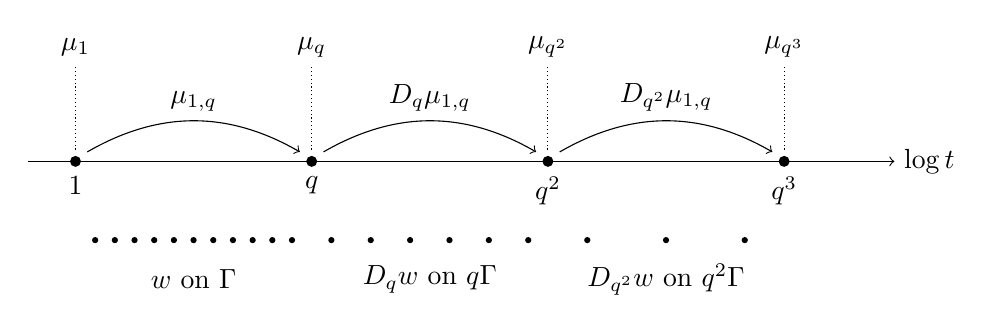
\begin{tikzpicture}[x=1cm,y=1cm,
  knot/.style={circle,fill,inner sep=1.4pt},
  gp/.style={circle,fill,inner sep=0.8pt}]
\draw[->] (-0.6,0) -- (10.4,0) node[right] {$\log t$};
\foreach \x/\lab in {0/1, 3/q, 6/q^2, 9/q^3} {
  \node[knot] at (\x,0) {};
  \node[below=2pt] at (\x,0) {$\lab$};
  \node at (\x,1.45) {$\mu_{\lab}$};
  \draw[densely dotted] (\x,0.15) -- (\x,1.2);
}
\foreach \x/\lab in {0/{\mu_{1,q}}, 3/{D_q\mu_{1,q}}, 6/{D_{q^2}\mu_{1,q}}} {
  \draw[->,bend left=30] (\x+0.15,0.12) to node[above] {$\lab$} (\x+2.85,0.12);
}
\foreach \k in {0,...,10} { \node[gp] at (0.25+0.25*\k,-1.0) {}; }
\foreach \k in {0,...,5} { \node[gp] at (3.25+0.5*\k,-1.0) {}; }
\foreach \k in {0,...,2} { \node[gp] at (6.5+1.0*\k,-1.0) {}; }
\node at (1.5,-1.5) {$w$ on $\Gamma$};
\node at (4.5,-1.5) {$D_qw$ on $q\Gamma$};
\node at (7.5,-1.5) {$D_{q^2}w$ on $q^2\Gamma$};
\end{tikzpicture}
\caption{A pyramid on the scale axis, drawn on a logarithmic scale. Levels are stored at the knots
$q^n$, and the knot kernels $\mu_{q^n}$ stand above them. The octave steps between consecutive
knots form the ladder, each step the dilate of $\mu_{1,q}$ by covariance
(Definition~\ref{def:knots-and-ladder}). Below, a grid pyramid applies one mask $w$ on a lattice
$\Gamma$, dilated to $D_{q^n}w$ on $q^n\Gamma$ at every level
(Definition~\ref{def:exact-grid-pyramid}). It is exact when a family continuous in scale and
covariant under $q$ has these steps as its ladder. Four objects are kept apart: the kernel
$\mu_t = \mu_{0,t}$ from the scale $0$ to $t$, the step $\mu_{s,t}$ from $s$ to $t$, a mask on a
lattice, and the samples of a continuum density. The input on the finest grid is read as the image
at the scale $1$. Level $n$ then applies the steps from $1$ to $q^n$, whose convolution is the
equivalent weight $W_n$ of Proposition~\ref{prop:equivalent-weights}. The knot kernel $\mu_{q^n}$
would also apply the smoothing below the scale $1$.}
\label{fig:pyramid-schematic}
\end{figure}

\paragraph{Contributions.} The answers, each proved in the section named, are the following.
\begin{enumerate}
\item \emph{Which families a pyramid can sample} (Section~\ref{ch:pyramid}). The dilations under
which a symmetric family is covariant form a closed group, so there are three cases: the identity
alone, the powers of one ratio $q$, or every dilation (Lemma~\ref{lem:family-dilations}). For a
fixed ratio $q$ the families therefore form three nested \emph{strata}: every symmetric family
(stratum~1), those covariant under the powers of $q$ (stratum~2), and those covariant under every
dilation (stratum~3). The strata depend on $q$, while the three cases of the group do not. The
pyramids are stratum~2: a \emph{pyramid} here is a family of stratum~2 read at its knots. The
computation that smooths and subsamples is called the computed pyramid, and the ladder of a mask on
a lattice a grid pyramid (Definition~\ref{def:exact-grid-pyramid}). For isotropic families each stratum is described by the
Gaussian part of the kernels and by their \Levy{} measures, which record the jumps, and each stratum
is strictly larger than the next (Theorems~\ref{thm:lattice-strata}
and~\ref{thm:lattice-strata-strict}). An isotropic family is fixed by its marginal on one axis
(Lemma~\ref{lem:reduction-keeps-stratum}). The line does not say which of its families extend to
$\RR^d$. The line's examples of the lower strata do not: in $d \ge 2$ no line exponent with
an atom in its \Levy{} measure is the marginal of a rotation-invariant infinitely divisible law
(Proposition~\ref{prop:what-does-not-lift}). The isotropic classes of one ratio shrink strictly as
the dimension grows (Proposition~\ref{prop:what-does-not-lift-chain}), as the fully covariant ones
do.

In stratum~2 the ladder fixes the kernels at the knots. The kernel at a knot is the convolution of all
the rungs below it, a limit, which is Burt's equivalent weighting function run downward in scale. The kernels between the knots are not fixed by the ladder. A
symmetric law other than a point mass is the octave step of such a family exactly when it is
infinitely divisible and has a logarithmic moment, $\int\log_+|x|\,\varrho(dx) < \infty$
(Proposition~\ref{prop:ladder-knot-kernel}). A law is \emph{infinitely divisible} when, for every
$n$, it is the $n$-fold convolution power of some law (Section~\ref{subsec:cited-sato}). For laws
this criterion is a theorem of Maejima and Ueda \cite[Thm.~3.3, p.~353]{maejima2009stochastic}. No law of
bounded support other than a point mass is a step $\mu_{s,t}$ of any family. The cascade and
continuity in scale exclude it, with no symmetry, covariance or nondegeneracy assumed
(Proposition~\ref{prop:no-bounded-step}). The proof joins two facts. The steps of a family are
infinitely divisible (Lemma~\ref{lem:steps-infinitely-divisible}; for processes
\cite[Thm.~9.1, p.~47]{sato1999levy}), and an infinitely divisible law other than a point mass has
unbounded support (Theorem~\ref{thm:cited-A46}). So the finite masks of the classical pyramids are the
octave steps of no family. A nonnegative one is excluded by that proposition. One with a negative
weight is excluded from the start, since every step of a family is a probability law.

\item \emph{The line and its grids} (Section~\ref{sec:line-theory}). On a grid $h\ZZ$ the criterion
becomes a criterion for masks: a symmetric probability mask other than $\delta_0$ has an exact
pyramid exactly when it is infinitely divisible
with a logarithmic moment, and the kernel at the knots is then unique. Continuity in scale forces
the infinite divisibility, through the steps of the family. Such a pyramid lies in
stratum~2 and never in stratum~3, since no family covariant under every dilation has a symmetric
lattice law other than $\delta_0$ as a step. The sampled Laplace mask, the two-sided exponential
density sampled on the grid, has an exact pyramid for every $q > 1$. No mask of bounded support has
one, the binomial and B-spline masks among them
(Proposition~\ref{prop:grid-pyramids-infinitely-divisible}). The sampled Laplace mask is applied by
one forward and one backward first-order recursion. For a fixed spacing, the sampled Laplace
kernels form an \emph{exact cascade} on the grid: the step between any two of them is again a
positive grid kernel of unit mass. This is a use of the word outside the three senses of
Definition~\ref{def:exact-senses}, which are these:
(i) a computation whose arrays are the kernels they stand for;
(ii) a family of grid kernels in which every $q$-th value of a member, renormalized, is a member;
(iii) a pyramid whose ladder is that of a continuous covariant family.
The word \emph{exact} in \emph{exact grid pyramid} is sense (iii). For an integer $q \ge 2$, the \Matern{} pyramid of
Section~\ref{ch:matern} computed by these recursions with decimation equals the samples of its
continuum steps at the first level, and differs from them at every later level, for every spacing
(Proposition~\ref{prop:sampled-laplace-exact}).

\item \emph{The \Matern{} pyramid and its selection} (Section~\ref{ch:matern}). The principle that
replaces the count of extrema is the maximum principle of an implicit Euler step of the heat
equation. At a local maximum of the output, the output does not exceed the input. At a local
minimum it is not below it (Definition~\ref{def:implicit-euler-principle}). Label the scales so that dilating
the kernel at $t$ by $q$ gives the kernel at $qt$. Required of every octave step, from every scale $t$ to $qt$, and for every smooth rapidly decreasing input, the principle singles out
one isotropic family covariant under $q$, up to a relabelling in the group $\mathcal{G}_q$ of
Lemma~\ref{lem:family-dilations}(3), which keeps that labelling. This is the \emph{\Matern{} pyramid}
(Theorem~\ref{thm:selection-stratum-two}(2)). In the labelling of Theorem~\ref{thm:matern-pyramid}, its octave step from $t$ to $qt$ is one implicit Euler
step of the heat equation, the Bessel potential $(I - c^2t^2\Delta)^{-1}$ with a constant $c > 0$,
so the step size grows by $q^2$ per octave (Theorem~\ref{thm:matern-pyramid}). The selected family
is covariant under every dilation (Theorem~\ref{thm:matern-pyramid}(1)). So it lies in stratum~3,
among the families that the isotropic paper classifies, although only covariance under $q$ was
required. The difference of the
levels $t$ and $qt$ is $-c^2t^2$ times the Laplacian of the coarser one. So for this family the
Laplacian pyramid of Burt and Adelson, read on the continuum before decimation, is a Laplacian
(Proposition~\ref{prop:laplacian-pyramid}). The selection rests on the stage lemma: a
rotation-invariant law other than $\delta_0$ that has the principle is a Bessel potential
(Proposition~\ref{prop:stage-lemma}). Among symmetric rotation-invariant laws the principle
therefore holds exactly for the Bessel potentials, and every Gaussian step fails it (Theorem~\ref{thm:selection-stratum-two}(4)). The
principle is a property of one step, and the theorem requires it of the octave steps only. A step
of the \Matern{} pyramid from $s$ to $t$ has it only when $t = qs$
(Theorem~\ref{thm:selection-stratum-two}(3)), and no symmetric family has it at every step
(Proposition~\ref{prop:principle-other-readings}(2)). The count of extrema does not select among the families with
absolutely continuous steps in the plane, since one step of every absolutely continuous law can
create a local maximum
(Proposition~\ref{prop:creation-plane}).

\item \emph{Exact pyramids on a lattice in $d \ge 2$ are not isotropic} (Section~\ref{ch:price}). In every dimension, a
symmetric probability mask on a lattice, other than a point mass, has an exact pyramid exactly when it is
infinitely divisible with a logarithmic moment (Proposition~\ref{prop:exact-masks}). The
criterion does not involve $q$, so exactness is a property of the mask alone. Such a mask has
unbounded support, so a pyramid that truncates its mask is not exact. The resolvent masks of the
discrete Helmholtz operators meet the criterion (Proposition~\ref{prop:resolvent-masks-exact}). In
$d \ge 2$ no exact pyramid whose mask is carried by a lattice is isotropic
(Proposition~\ref{prop:grid-pyramid-not-isotropic}). The same holds when the dilation is an
invertible matrix, which may also turn the lattice, as in the quincunx and hexagonal pyramids
(Proposition~\ref{prop:expanding-grid-pyramid-not-isotropic}). The reason
is where the jumps lie. An infinitely divisible lattice law has no Gaussian part, and its \Levy{}
measure lies on the lattice (Lemma~\ref{lem:lattice-infinitely-divisible}). Through the knot
product the same holds for the family: every kernel at a positive scale has no Gaussian part and a
nonzero \Levy{} measure carried by a countable set
(Proposition~\ref{prop:grid-pyramid-not-isotropic}(1)). In $d \ge 2$ a rotation-invariant law with
a nonzero \Levy{} measure cannot be carried that way. So in $d \ge 2$ no kernel at a positive scale
of any family carrying an exact pyramid on a lattice is rotation invariant
(Proposition~\ref{prop:grid-pyramid-not-isotropic}(2)), and no such pyramid is isotropic. The
obstruction needs continuity in scale as well as the lattice. For a mask with an exponential
moment, as every finite mask has, the knot relation
$D_q\mu_1 = \mu_1 * w$ alone excludes isotropy: its only rotation-invariant solution is $\delta_0$
(Proposition~\ref{prop:no-isotropic-refinable-finite-mask}). For some masks of infinite support it
does not, and no family continuous in scale carries those masks
(Proposition~\ref{prop:band-limited-refinable-mask}).
Isotropy
is defined through a carrying family, so a grid pyramid without one is not isotropic in this sense
either. The continuum \Matern{} pyramid,
with no lattice, is isotropic.

Exact pyramids on a lattice exist in every dimension. One is the frame \Matern{} pyramid on the
grid, whose mask is the product of sampled Laplace masks along the coordinate axes
(Proposition~\ref{prop:grid-pyramid-not-isotropic}). In $d \ge 2$ its mask fails the implicit-Euler
principle on every finite symmetric neighbourhood, while each pass along one axis has it on every
such neighbourhood that contains the two neighbours on that axis
(Proposition~\ref{prop:grid-frame-step-not-selected}). Local maxima are created on the grid as well.
Read them on a finite symmetric neighbourhood that contains the axis neighbours. Then, in $d \ge 2$
and for an integer $q \ge 2$, three masks each create a local maximum across one level of the
decimated pyramid, at every level, for an input that depends on the level: the frame mask, the resolvent mask of the $(2d+1)$-point
Laplacian, and the tensor power of the binomial mask (Propositions~\ref{prop:creation-grid-masks}
and~\ref{prop:binomial-records}). The section ends with the resolvent kernels of the
$(2d+1)$-point Laplacian on $h\ZZ^d$ and of the nine-point Laplacian on $h\ZZ^2$, whose convolution
powers form exact cascades on the grid (Propositions~\ref{prop:discrete-helmholtz}
and~\ref{prop:nine-point-family}).
\end{enumerate}

\paragraph{Relation to the literature.} Each octave of the \Matern{} pyramid is one implicit heat
step, and the step sizes grow geometrically. Such sequences of implicit steps occur in nonstationary
iterated Tikhonov regularization \cite[pp.~38--39]{hanke1998nonstationary}, read there as diffusion time in
\cite[p.~98]{radmoser2000scale}, and in multiscale edge-preserving decompositions
\cite[\S 3.1, (13)--(14)]{farbman2008edge}. Scherzer and Weickert read one regularization step as
one implicit diffusion step and prove its extremum principle
\cite[p.~43; Lemma~6, p.~53]{scherzer2000relations}.
Nielsen, Florack and Deriche read the first-order regularization filter as the heat equation with a
remapped scale, and compute products of such filters recursively
\cite[pp.~296--298]{nielsen1997regularization}.
Decimation between the implicit steps, a covariant family through them, and its uniqueness up to
the gauge under the implicit-Euler principle were not found in that literature. Decimation between explicit steps is Burt's \cite[\S 4, p.~29]{burt1981fast}. The
covariance condition under one ratio is, for laws, semi-selfdecomposability
\cite[Def.~3.1, p.~19]{maejima1998semi}, \cite[Def.~15.1, p.~90]{sato1999levy}, and the strata are
its reading for scale spaces. In probability theory two-parameter families of laws with the
cascade are called convolution hemigroups. Becker-Kern treats those covariant under a linear map,
at every ratio and at the powers of one ratio \cite[p.~574]{becker-kern2003stable}. For laws, the criterion for an octave step, an infinitely divisible
law with a logarithmic moment, is a theorem of Maejima and Ueda on semi-selfdecomposable laws of one
span \cite[Thm.~3.3, p.~353]{maejima2009stochastic}. This paper adds its reading as the ladder of a
family, the kernels between the knots, and their use in the selection. Multiresolution analysis \cite[(2)--(8), p.~676]{mallat1989theory} is the axiomatic dyadic
neighbour, by projection rather than smoothing. Lindeberg's scale space for discrete signals
\cite{lindeberg1990scalespace} lies in stratum~1 and not in stratum~2: it is covariant under no
dilation (Section~\ref{sec:line-theory}). Lindeberg's time-causal limit kernel is an infinite
convolution of first-order integrators whose time constants fall in a fixed ratio, his distribution
parameter. It is covariant under the integer powers of that ratio
\cite[\S 5, p.~62; (47), p.~63]{lindeberg2016time}. It is
the nearest precedent in scale-space theory for covariance under one ratio. On the line the kernel
$\mu_t$ of the \Matern{} pyramid is the limit kernel of ratio $q$ and time constants $ctq^{-i}$,
$i \ge 1$, convolved with its reflection. In every dimension $\mu_t$ is a mixture of Gaussians whose
variance has the law of the limit kernel of ratio $q^2$ (Section~\ref{ch:matern}). The \Matern{} pyramid takes its name from the \Matern{}
covariances, whose transforms are powers of the transform of its octave step [\sscite{whittle1954stationary}, p.~448; \sscite{lindgren2011explicit}, (2), p.~426].
Lowe's pyramid of scale-invariant features smooths by Gaussian steps of ratio $2^{1/s}$ within each
octave and subsamples by $2$ between octaves \cite[pp.~6--7]{lowe2004distinctive}. Read as in this
paper, it computes the steps of the Gaussian family, with sampled kernels. Lindeberg's discrete
approximations of Gaussian smoothing leave subsampling aside \cite[p.~762]{lindeberg2024discrete}.
Other pyramids change the ratio or the smoothing. Crowley resamples by $\sqrt2$, onto a lattice
turned by $45^\circ$ \cite[\S 3.3.2, p.~32]{crowley1981representation}. The hybrid pyramids of
Lindeberg and Bretzner take several smoothing steps between two subsamplings by~$2$
\cite[\S 3.1]{lindeberg2003real}. The polynomial spline pyramids of Unser, Aldroubi and Eden reduce
and expand with binomial filters, and for cubic splines they are close to Burt's
\cite[\S IV.B, p.~370]{unser1993polynomial}.
That Gaussian smoothing can create a local extremum in the plane is classical, with an example of
Lifshitz and Pizer \cite[\S 4.1, p.~101]{lindeberg1994scale}, \cite[p.~369]{damonLocalMorseTheory1995}.
From that example Lindeberg argues, without a theorem, that every non-trivial kernel on $\RR^2$ or
$\ZZ^2$ can create one \cite[\S 4.1, p.~101]{lindeberg1994scale}. Here it is proved for one step of every
absolutely continuous law, across every octave step of the \Matern{} pyramid, and across an octave
step of the Gaussian ladder at any prescribed scale (Proposition~\ref{prop:creation-plane}).

How the isotropic members of these families are computed in the plane, where the octave step of the
\Matern{} pyramid does not split into first-order passes along fixed directions
(Lemma~\ref{lem:no-first-order-factorization}), is a question for further work.
% TODO(module computation): cite the computation paper when released.

\paragraph{How the paper is organized.} Section~\ref{sec:trust} says what is machine-checked.
Section~\ref{ch:cited} restates what is used from the author's earlier papers, at their released
numbers, and the facts of the literature. Sections~\ref{ch:pyramid}--\ref{ch:price} prove the four
contributions in order, and Section~\ref{sec:line-theory} also reads the strata of
Section~\ref{ch:pyramid} on the line. Section~\ref{sec:discussion} says what the results do not
cover and answers four questions they raise. The supplement states the strata on the line in the line's own
terms. It also treats the families of stratum~2 on the line in detail: how the members with one
ladder differ inside an octave, an entropy that, read in a fixed gauge, selects the similarity
member $\Psi_t = \Psi_1(t\,\cdot)$ when the ladder has one and no Gaussian part, and three clusters of examples that set the classical pyramids against
the axioms. The supplement is part of the paper. Some proofs in
Sections~\ref{sec:line-theory}--\ref{ch:price} cite its statements on the line. The proof of Theorem~\ref{thm:matern-pyramid}, which constructs
the \Matern{} pyramid, rests on its line case there (Theorem~\ref{thm:matern-pyramid-line}).

\subsection{What is machine-checked}
\label{sec:trust}
% trust base: begin
% This subsection is the statement of the trust base (article-kit WRITING.md section 4). Its
% inventory, the table of which statement rests on which cited fact, is Appendix A. The admitted
% entries are those of blueprint/AXIOMS.md with a Lean axiom (blueprint/trust-boundary.txt).
The numbered statements of Sections~\ref{ch:pyramid}, \ref{sec:line-theory}, \ref{ch:matern}
and~\ref{ch:price} and of the supplement have formal counterparts in the Lean~4 proof assistant, on
its mathematical library Mathlib. All of them are machine-checked except one step of
Proposition~\ref{prop:grid-pyramids-infinitely-divisible}(4): that the binomial masks other than
$\tfrac1{16}[1,4,6,4,1]$ and the B-spline samples are symmetric masks of bounded support, which its
proof shows in print. For $\tfrac1{16}[1,4,6,4,1]$ that step is machine-checked too. Three
statements are proved in print only, in whole or in part:
\begin{itemize}
\item Proposition~\ref{prop:expanding-grid-pyramid-not-isotropic}, that in $d \ge 2$ no exact grid
pyramid whose dilation is an invertible matrix is isotropic;
\item clause (3) of Proposition~\ref{prop:grid-pyramid-singular-kernels}, that for an integer ratio
the kernels of an exact grid pyramid on $h\ZZ^d$ are singular. Its clauses (1) and (2) have Lean
proofs, which Appendix~\ref{app:verification} names;
\item Proposition~\ref{prop:band-limited-refinable-mask}, the band-limited mask with a
rotation-invariant refinable law, whose formal proof would need Poisson summation on $\ZZ^d$.
\end{itemize}
The formal statements of what is proved in print only are written, in a skeleton library that the
formal development does not import, and not proved. For each other lemma,
proposition, theorem and corollary there, Lean checked that the formal statement follows from the
formal definitions, Lean's three logical axioms (\texttt{propext}, \texttt{Classical.choice},
\texttt{Quot.sound}) and the cited facts named below. A proof is said to use \emph{no cited fact}
when Lean's report lists those three axioms only. The sentence that closes many proofs, that every
step is machine-checked, means this of the formal counterpart of the statement proved. It does not
certify each step of the printed argument. The formal statements, of this paper's results and of the cited facts
alike, were compared with the printed ones by AI agents, statement by statement, and so were the
formal definitions. The statement on
the use of AI at the end of the paper says how the work was done.

The connecting prose between the numbered statements is not formalized, and a mathematical claim
made there is covered only through the numbered statement it cites.
The numerical statements of Section~\ref{sec:line-theory} (the sizes of errors measured on the grid)
are computed by the scripts they name, and no numbered statement rests on them. One argument there
is proved in print only: that the sampled Gaussian kernels of standard deviations $0.5$ and $0.6$ on
$\ZZ$ are joined by no probability law. It rests on two moments computed by the script, as sums cut at
$|k| \le 5$ with a tail below $10^{-18}$, which can be checked by hand.

The development imports two earlier formal developments, each at a pinned release. The first is the
library \texttt{ScaleSpaceCore}, the shared core first released with the line paper
\progpaper{V-line v0.1}, here at its later tag \texttt{v0.5.0}. It supplies the operator axioms, the representation of the line's operators
as convolutions, the classification on the line and the Bessel function $K_\nu$. It declares no
axiom: where it needs a cited fact, it takes it as a hypothesis, which this development discharges
from the cited facts below. The second is the formal development of the affine paper
\progpaper{affine v0.1}, at that release.

The cited facts are the statements of Section~\ref{sec:cited-literature} and those restated from the
author's earlier papers in Section~\ref{sec:cited}, each stated as a numbered theorem with the page of
its source. Nine of them are \emph{admitted interfaces}: the formal development takes them as
axioms, fourteen axioms in all. Section~\ref{supp:axioms} of the supplement prints the fourteen as
the Lean source states them.
\begin{itemize}
\item From Sato \cite{sato1999levy}: the \Levy{}--Khintchine representation
(\ledger{A39}, three axioms), Khintchine's theorem on null arrays (\ledger{A41}), the infinite divisibility of self-decomposable and
semi-selfdecomposable laws and of their residuals (\ledger{A43}, three axioms), the polar form of a
self-decomposable \Levy{} measure (\ledger{A45}), the unbounded support of an infinitely divisible
law (\ledger{A46}), the lattice-carried infinitely divisible laws on the line (\ledger{A48}), and the
$g$-moment theorem (\ledger{A49}).
\item The \Polya{} frequency clause of the selection module \progpaper{V-selection v0.1}
(\ledger{A22}, two axioms, one per clause used), a classical fact of Schoenberg's that Karlin
proves \cite{karlin1968total}, and Schoenberg's representation of \Polya{}
frequency densities (\ledger{A24}), admitted only for its identity on the imaginary axis, which is
all the proofs read. The counts along the projections of the \Matern{} pyramid,
Theorem~\ref{thm:matern-pyramid}(3), read both.
\end{itemize}
Six of the fourteen axioms are axioms of the affine paper's development, which this development
uses under their own names: the three of \ledger{A39}, that of \ledger{A41}, that of \ledger{A45}
and the first clause of \ledger{A43}.

Of the nineteen cited facts that are not admitted, twelve are theorems of the formal development.
The classification on the line (\ledger{A4}), the uniqueness of the data of a line exponent
(\ledger{A9}), the counting clause of the selection module (\ledger{A23}), the characterization of
semi-selfdecomposable laws (\ledger{A44}) and the absence of zeros of an infinitely divisible
transform (\ledger{A40}) are proved from the admitted ones. The classification in $\RR^d$
(\ledger{A31}), the realization of every gauge and nonzero admissible exponent by a family
(Theorem~\ref{thm:cited-A34}) and the polar description of the isotropic exponents (\ledger{A35})
are theorems of
the affine paper's development, the second with no cited fact. The representation of the line's
operators (Theorem~\ref{thm:cited-A1}), the triplet of a linear image (\ledger{A42}), the
submultiplicativity of $\log(|x| \vee e)$ (Theorem~\ref{thm:cited-A50}) and the integral
representation of $K_\nu$ (Theorem~\ref{thm:cited-A51}) are proved with no cited fact. The other
seven, which
Appendix~\ref{app:verification} names, are stated for the reader and read by no formal proof of
this paper. The prose of Section~\ref{ch:matern} uses two of them, the Bernstein facts, to explain
the kernels. They are not proved in Lean: their statements are typed, without proof, in a skeleton
library that the formal development does not import.

Each admitted fact is stated as its source states it, or narrower. Where the formal statement is
narrower than the page, the statement of Section~\ref{ch:cited} says so.

As an example of Lean's report, clause (2) of Theorem~\ref{thm:lattice-strata}, the description of
stratum~2, rests on the \Levy{}--Khintchine representation and Khintchine's theorem:
% printed at 2fc473a
\begin{verbatim}
'Pyramids.lattice_strata_2' depends on axioms: [propext,
 AffineHemigroup.khintchine_null_array,
 AffineHemigroup.levy_khintchine_converse,
 AffineHemigroup.levy_khintchine_exists,
 AffineHemigroup.levy_khintchine_unique,
 Classical.choice,
 Quot.sound]
\end{verbatim}
Table~\ref{tab:headline} lists two declarations for clause (2) of the selection theorem,
Theorem~\ref{thm:selection-stratum-two}, and neither uses a cited fact. The theorem as a whole reads
the cited facts that Table~\ref{tab:statements} gives for it. Table~\ref{tab:headline}, in
Appendix~\ref{app:verification}, lists the cited facts that Lean reports for each of the headline
declarations, and Table~\ref{tab:statements} there does the same for every numbered statement.
Table~\ref{tab:axioms} maps the fourteen axioms to the nine admitted facts.
% trust base: end

% Transcribed from blueprint/src/parts/02-cited-facts.tex.
\section{What is cited}
\label{ch:cited}

This paper rests on five releases of the author's earlier work, cited at the printed number and
page. The line paper \progpaper{V-line v0.1} states the axioms on the line and classifies the
families that satisfy them. Two companion papers were released with it. The first, its
\emph{cone module} \progpaper{V-cone v0.1}, describes these families as a convex cone, with their
generators and their computation on the line. The second, its \emph{selection module}
\progpaper{V-selection v0.1}, treats locality and the non-creation of extrema. The isotropic
paper \progpaper{iso v0.1} carries the axioms and the classification to $\RR^d$. The affine paper
\progpaper{affine v0.1} supplies the frame families, which the supplement uses for the separability
of the classical kernels.

Section~\ref{sec:cited} states what this paper takes from these releases: the axioms, the two
classifications and the other statements that the proofs use.
Section~\ref{sec:cited-literature} states the facts of the literature: the \Levy--Khintchine
theory of infinitely divisible laws, Bernstein functions, \Polya{} frequency densities and one
integral of a Bessel function. Each fact of these theories that a proof takes as given is a
numbered theorem, its source and page
are named just before it, and a proof that uses it refers to it. Standard measure theory and
probability, such as \Levy{}'s continuity theorem, Steinhaus's theorem and the Radon--Nikodym
theorem, are used without a number.
Theorems~\ref{thm:cited-A30}, \ref{thm:cited-A13}, \ref{thm:cited-A19} and~\ref{thm:cited-A20}
orient the reader, and the remarks of Section~\ref{sec:line-theory} and the supplement compare
with the last three.

\subsection{The released modules: axioms, classifications and notation}
\label{sec:cited}

\subsubsection{The axioms on the line}
\label{subsec:cited-line}

A scale space keeps a record of a signal at every scale $t \ge 0$, the signal itself at $t = 0$,
and an operator $\Phi_{s,t}$ takes the record at scale $s$ to the record at the coarser scale $t$.
The cascade (A6) requires that two such steps compose to one. It replaces the semigroup law
$\Phi_{t+s} = \Phi_t\Phi_s$ of the classical theory, which ties the scale to a fixed additive
parametrization, and a family with (A6) is a \emph{hemigroup}. Covariance (A8) requires that a dilation
of the signal only relabel the scales, and (ND) excludes the identity.

% shared with blueprint def:cascade-measurement-family
\begin{definition}[symmetric cascade measurement families]
\label{def:cascade-measurement-family}

A \emph{symmetric cascade measurement family} is a family of linear operators
$\Phi_{s,t} : L^1(\RR) \to L^1(\RR)$, $0 \le s \le t < \infty$, such that
\begin{itemize}
\item[(A1)] each $\Phi_{s,t}$ is a bounded operator on $L^1(\RR)$;
\item[(A2)] $\Phi_{s,t}$ commutes with every translation $f \mapsto f(\cdot - a)$, $a \in \RR$;
\item[(A3)] $\Phi_{s,t}$ commutes with the reflection $f \mapsto f(-\,\cdot)$;
\item[(A4)] $\Phi_{s,t}$ maps nonnegative functions to nonnegative functions;
\item[(A5)] $\int\Phi_{s,t}f = \int f$ for every nonnegative $f \in L^1(\RR)$;
\item[(A6)] $\Phi_{t,t} = \Id$, and $\Phi_{s,t}\Phi_{r,s} = \Phi_{r,t}$ for all $r \le s \le t$
(the cascade);
\item[(A7)] for every $f \in L^1(\RR)$ the map $(s,t) \mapsto \Phi_{s,t}f$ is continuous from
$\{0 \le s \le t\}$ to $L^1(\RR)$;
\item[(A8)] there is a family $(S_\lambda)_{\lambda > 0}$ of increasing bijections of $[0,\infty)$
with $\mathcal{D}_\lambda\Phi_{s,t} = \Phi_{S_\lambda s, S_\lambda t}\mathcal{D}_\lambda$ for all
$0 \le s \le t$ and all $\lambda > 0$, where $(\mathcal{D}_\lambda f)(x) := \lambda^{-1}f(x/\lambda)$
(scale covariance);
\item[(ND)] $\Phi_{s,t} \ne \Id$ whenever $s < t$ (nondegeneracy).
\end{itemize}
\end{definition}

The first consequence of the axioms is that each operator is a convolution
\prog{V-line v0.1}{Lemma~4.1, pp.~22--23}.

% shared with blueprint thm:cited-A1
\begin{theorem}[each operator is a convolution]
\label{thm:cited-A1}

Let $\Phi_{s,t}$, $0 \le s \le t$, be linear operators on $L^1(\RR)$ with (A1), (A2), (A4) and
(A5) of Definition~\ref{def:cascade-measurement-family}. Then for each pair $0 \le s \le t$ there
is a unique probability measure $\mu_{s,t}$ on $\RR$ with
\[
  \Phi_{s,t}f = \mu_{s,t} * f, \qquad f \in L^1(\RR);
\]
under (A3) it is symmetric, invariant under $x \mapsto -x$. Conversely, every symmetric
probability measure on $\RR$ defines, by convolution, an operator with (A1)--(A5).
\end{theorem}

\begin{proof}
Existence and uniqueness are \prog{V-line v0.1}{Lemma~4.1, p.~22}, with the proof printed there
and proved again in the formal development:
under (A1), (A2), (A4) and (A5) each $\Phi_{s,t}$ is the convolution with exactly one probability
measure $\mu_{s,t}$, the equation $\Phi_{s,t}f = \mu_{s,t} * f$ holding in $L^1(\RR)$, that is,
almost everywhere.

For the symmetry, write $f^-(x) := f(-x)$ and $\mu^-$ for the image of $\mu = \mu_{s,t}$
under $x \mapsto -x$. The change of variables $y \mapsto -y$ gives
$\mu^- * f = (\mu * f^-)^-$ for every $f \in L^1(\RR)$. By (A3),
$\Phi_{s,t}f^- = (\Phi_{s,t}f)^-$, so $\mu^- * f = (\Phi_{s,t}f^-)^- =
\Phi_{s,t}f = \mu * f$ for every $f$. A probability measure is determined by its convolution
operator on $L^1(\RR)$: with $g(x) := (2\pi)^{-1/2}e^{-x^2/2}$, the transform of $\mu * g$ is
$\widehat\mu\,\widehat g$, and $\widehat g$ has no zero. So $\mu^- = \mu$.

For the converse let $\mu$ be a symmetric probability measure on $\RR$. The map
$f \mapsto \mu * f$ is linear, and $\|\mu * f\|_1 \le \|f\|_1$ by Tonelli's theorem, so it is a
bounded operator on $L^1(\RR)$, which is (A1). Since
$(\mu * f(\cdot - a))(x) = \int f(x - a - y)\,\mu(dy) = (\mu * f)(x - a)$, it commutes with
translation, which is (A2). Since $\mu^- = \mu$, the identity of the previous paragraph reads
$\mu * f^- = (\mu * f)^-$, which is (A3). If $f \ge 0$ almost everywhere, then
$\mu * f \ge 0$ almost everywhere, which is (A4), and Fubini's theorem gives
$\int \mu * f = \mu(\RR)\int f = \int f$, which is (A5).

Every step is machine-checked, the released lemma's included, and no fact of the literature is
cited.
\end{proof}

Under (A1)--(A7) the transform of the kernel is $\widehat\mu_{s,t} = e^{-g_{s,t}}$ with
\[
  g_{s,t}(\omega) = a(s,t)\,\omega^2 + \int_{(0,\infty)}(1 - \cos\omega x)\,\varpi_{s,t}(dx),
  \quad a(s,t) \ge 0, \quad \int_{(0,\infty)}\min(1, x^2)\,\varpi_{s,t}(dx) < \infty
\]
\prog{V-line v0.1}{Thm.~5.2, p.~26}. So every \emph{step} $\mu_{s,t}$ is a
symmetric \emph{infinitely divisible} law: for every $n$ it is the $n$-fold convolution power of
some law. The exponent of a step has a Gaussian part
$a(s,t)\omega^2$ and a jump part, and $\varpi_{s,t}$, its \emph{\Levy{} measure} folded onto
$(0,\infty)$, counts the jumps by their length. The pair $(a, \varpi)$ of such an exponent is
determined by the function \prog{V-line v0.1}{Prop.~2.3(3), p.~9}. The proof reads the
\Levy--Khintchine representation, Theorem~\ref{thm:cited-A39} of
Section~\ref{sec:cited-literature}.

% shared with blueprint thm:cited-A9
\begin{theorem}[the folded \Levy--Khintchine pair is unique]
\label{thm:cited-A9}

Let $a, a' \ge 0$, and let $\nu$ and $\nu'$ be measures on $(0,\infty)$ with
$\int_{(0,\infty)}\min(1, x^2)\,\nu(dx) < \infty$ and
$\int_{(0,\infty)}\min(1, x^2)\,\nu'(dx) < \infty$. If
\[
  a\,\omega^2 + \int_{(0,\infty)}(1 - \cos\omega x)\,\nu(dx)
  = a'\,\omega^2 + \int_{(0,\infty)}(1 - \cos\omega x)\,\nu'(dx)
  \qquad\text{for every } \omega \in \RR,
\]
then $a = a'$ and $\nu = \nu'$.
\end{theorem}

\begin{proof}
For a pair $(a, \nu)$ as in the statement let $\tilde\nu$ be the symmetric measure on $\RR$ with
$\tilde\nu(\{0\}) = 0$ and $\tilde\nu(B) = \tfrac12\nu(B \cap (0,\infty)) +
\tfrac12\nu(-B \cap (0,\infty))$. Then $\int\min(x^2, 1)\,\tilde\nu(dx) =
\int_{(0,\infty)}\min(x^2, 1)\,\nu(dx) < \infty$, so $(2a, \tilde\nu, 0)$ is a generating triplet
on $\RR$. In its \Levy--Khintchine bracket the imaginary part of the integrand,
$\sin\omega x - \omega x\mathbf 1_{|x| \le 1}$, is odd and $\tilde\nu$-integrable, so it integrates
to $0$. The real part $\cos\omega x - 1$ is even, so its $\tilde\nu$-integral is
$-\int_{(0,\infty)}(1 - \cos\omega x)\,\nu(dx)$. With the Gaussian term
$-\tfrac12\cdot 2a\,\omega^2$ the bracket is $-\psi(\omega)$, where $\psi$ is the function of the
pair, $\psi(\omega) = a\omega^2 + \int_{(0,\infty)}(1 - \cos\omega x)\,\nu(dx)$.

By Theorem~\ref{thm:cited-A39}(iii) there is an infinitely divisible law $\mu$ on $\RR$ with the triplet
$(2a, \tilde\nu, 0)$, so $\widehat\mu = e^{-\psi}$. By hypothesis the pair $(a', \nu')$ has the
same function $\psi$. So by the first paragraph the triplet $(2a', \tilde\nu', 0)$ also represents
$\widehat\mu$ by the formula of Theorem~\ref{thm:cited-A39}(i). By Theorem~\ref{thm:cited-A39}(ii) the two triplets
are equal: $a = a'$ and $\tilde\nu = \tilde\nu'$. On $(0,\infty)$ the measure $\tilde\nu$ is
$\tfrac12\nu$, so $\nu = 2\tilde\nu|_{(0,\infty)} = 2\tilde\nu'|_{(0,\infty)} = \nu'$.

Every step is machine-checked, and the cited fact is \ledger{A39}(ii)--(iii), at $d = 1$.
\end{proof}

The full axioms produce a classical class of laws. By the cascade the kernel $\mu_{0,t}$ is the
kernel $\mu_{0,s}$ at a finer scale convolved with the step $\mu_{s,t}$. By covariance
$\mu_{0,s}$ is a dilate of $\mu_{0,t}$. So each kernel is a shrunken copy of itself convolved with a
law, which is the property the next definition names [\sscite{sato1999levy}, Def.~15.1, p.~90].

% shared with blueprint def:self-decomposable
\begin{definition}[self-decomposable and semi-selfdecomposable laws]
\label{def:self-decomposable}

Let $\mu$ be a probability measure on $\RR^d$. It is \emph{self-decomposable} if, for every
$b > 1$, there is a probability measure $\varrho_b$ on $\RR^d$ such that
\[
  \widehat\mu(z) = \widehat\mu(b^{-1}z)\,\widehat\varrho_b(z), \qquad z \in \RR^d.
\]
It is \emph{semi-selfdecomposable} if there are some $b > 1$ and some infinitely divisible
probability measure $\varrho_b$ with the same identity. Then $b$ is called a \emph{span} of $\mu$, and
$\varrho_b$ its \emph{residual}.
\end{definition}

With $c := b^{-1} \in (0,1)$ the identity reads
$\widehat\mu(\omega) = \widehat\mu(c\omega)\,\widehat\varrho_b(\omega)$: $\mu$ is the law of
$cX + Y$ with $X \sim \mu$ and $Y \sim \varrho_b$ independent. The exponents of the
symmetric self-decomposable laws on the line are those of the form
\begin{equation}
\label{eq:admissible-exponent}
  F(\omega) = a\,\omega^2 + \int_0^\infty(1 - \cos\omega x)\,\frac{k(x)}{x}\,dx
\end{equation}
with $a \ge 0$, $k : (0,\infty) \to [0,\infty)$ nonincreasing and
$\int_0^\infty\min(1, x^2)\,k(x)\,x^{-1}\,dx < \infty$ \prog{V-line v0.1}{Prop.~2.13, p.~13}, the
integrability being that of a \Levy{} measure. The classification of the line is the main theorem
of the line paper \prog{V-line v0.1}{Thm.~7.3, p.~37}.

% shared with blueprint thm:cited-A4
\begin{theorem}[the classification on the line]
\label{thm:cited-A4}

A family $(\Phi_{s,t})_{0 \le s \le t}$ of linear operators on $L^1(\RR)$ satisfies (A1)--(A8)
and (ND) of Definition~\ref{def:cascade-measurement-family} if and only if there are an increasing
bijection $\chi$ of $[0,\infty)$, the \emph{gauge}, and a function $F \not\equiv 0$ of the form
\[
  F(\omega) = a\,\omega^2 + \int_0^\infty(1 - \cos\omega x)\,\frac{k(x)}{x}\,dx,
\]
with $a \ge 0$, $k \ge 0$ nonincreasing and
$\int_0^\infty\min(1, x^2)\,k(x)\,x^{-1}\,dx < \infty$, such that $\Phi_{s,t}f = \mu_{s,t} * f$ with
\[
  \widehat\mu_{s,t}(\omega) = \exp\bigl(-[F(\chi(t)\omega) - F(\chi(s)\omega)]\bigr),
  \qquad 0 \le s \le t,\ \omega \in \RR.
\]
Conversely, for every such pair $(\chi, F)$ there are probability measures $\mu_{s,t}$ with
these transforms, and the operators $f \mapsto \mu_{s,t} * f$ satisfy (A1)--(A8) and (ND).
The pair $(\chi, F)$ is unique once $\chi(1) = 1$.
\end{theorem}

In the \emph{canonical gauge} $\chi = \mathrm{id}$ the kernel at scale $t$ has transform
$e^{-F(t\omega)}$, and the family is the \emph{similarity family} of $F$. The functions $F$ of the
form (\ref{eq:admissible-exponent}) are the \emph{admissible exponents}, and $(a, k)$ their
\emph{data}. They form a convex cone \prog{V-cone v0.1}{Lemma~2.7, p.~12}. The Gaussian is the
exponent with $k = 0$. The \Matern{} exponent $\gamma\log(1 + \omega^2)$ of index $\gamma$ has
$a = 0$ and $k(x) = 2\gamma e^{-x}$.

\subsubsection{The axioms in $\RR^d$}
\label{subsec:cited-d}

The isotropic paper carries the axioms from the line to $\RR^d$, with rotation invariance in place
of symmetry, and classifies the families that satisfy them. This subsection states both, since
Section~\ref{ch:pyramid} weakens the first and compares its strata with the second. Fix $d \ge 1$.
For a measure $\mu$ on $\RR^d$ write
$\widehat\mu(\omega) = \int e^{i\langle\omega, x\rangle}\,\mu(dx)$, and for a linear map $A$ of
$\RR^d$ write $A_*\mu$ for the image of $\mu$ under $x \mapsto Ax$.

% shared with blueprint def:isotropic-cascade-family
\begin{definition}[isotropic cascade families]
\label{def:isotropic-cascade-family}

Let $d \ge 1$. An \emph{isotropic cascade family in dimension $d$} is a family
$(\mu_{s,t})_{0 \le s \le t}$ of probability measures on $\RR^d$ such that
\begin{itemize}
\item[(I1)] $\mu_{t,t} = \delta_0$, and $\mu_{r,t} = \mu_{s,t} * \mu_{r,s}$ whenever
$r \le s \le t$ (cascade);
\item[(I2)] for every $\omega \in \RR^d$ the map $(s,t) \mapsto \widehat\mu_{s,t}(\omega)$ is
continuous on $\{0 \le s \le t\}$ (continuity);
\item[(I3)] $Q_*\mu_{s,t} = \mu_{s,t}$ for every $Q \in \Orth(d)$ and every pair (rotation
invariance);
\item[(I4)] there is a family $(S_\lambda)_{\lambda > 0}$ of increasing bijections of
$[0,\infty)$ with $(\lambda I)_*\mu_{s,t} = \mu_{S_\lambda s, S_\lambda t}$ for every $\lambda > 0$
and every pair (dilation covariance);
\item[(ND)] $\mu_{s,t} \ne \delta_0$ whenever $s < t$ (nondegeneracy).
\end{itemize}
\end{definition}

The axioms are stated on the kernels. The isotropic paper also states them on operators on
$L^1(\RR^d)$, as (A1)--(A8) and (ND) with the rotations in place of the reflection
\prog{iso v0.1}{Def.~3.1, pp.~10--11}. The two definitions describe the same families, by the
next theorem \prog{iso v0.1}{Lemma~3.3, pp.~11--12}.

% shared with blueprint thm:cited-A30
\begin{theorem}[operators and kernels in dimension $d$]
\label{thm:cited-A30}

Let $d \ge 1$, and for a probability measure $\mu$ on $\RR^d$ and $f \in L^1(\RR^d)$ write
$(\mu * f)(x) := \int f(x - y)\,\mu(dy)$.
\begin{enumerate}
\item Let $\Phi$ be a linear operator on $L^1(\RR^d)$ that is bounded, commutes with every
translation $f \mapsto f(\cdot - a)$, $a \in \RR^d$, maps nonnegative functions to nonnegative
functions, and has $\int\Phi f = \int f$ for every nonnegative $f$. Then there is a unique
probability measure $\mu$ on $\RR^d$ with $\Phi f = \mu * f$ for every $f \in L^1(\RR^d)$.
Conversely, for every probability measure $\mu$ on $\RR^d$ the operator $f \mapsto \mu * f$ has
these four properties.
\item Let $\mu_n$ and $\mu$ be probability measures on $\RR^d$. Then
$\widehat\mu_n(\xi) \to \widehat\mu(\xi)$ for every $\xi \in \RR^d$ if and only if
$\mu_n * f \to \mu * f$ in $L^1(\RR^d)$ for every $f \in L^1(\RR^d)$.
\end{enumerate}
\end{theorem}

So (I1) is the cascade (A6), (I2) the continuity (A7) and (I4) the covariance (A8), with the same
bijections. (I3) is the rotation invariance, which in $\RR^d$ takes the place of the reflection
(A3). Let $\mathcal{A}_d$ be the set of admissible $F$ for
which $\omega \mapsto F(|\omega|)$, $\omega \in \RR^d$, is the exponent of a self-decomposable law
on $\RR^d$. Then $\mathcal{A}_1$ is the whole cone of admissible exponents and
$\mathcal{A}_{d+1} \subseteq \mathcal{A}_d$ \prog{iso v0.1}{Prop.~2.6, p.~8}. The classification
in $\RR^d$ is the main theorem of the isotropic paper \prog{iso v0.1}{Thm.~3.6, p.~13}.

% shared with blueprint thm:cited-A31
\begin{theorem}[the classification in $\RR^d$]
\label{thm:cited-A31}

Let $d \ge 1$, and let $\mathcal{A}_d$ be the set of admissible exponents $F$ (of the form
(\ref{eq:admissible-exponent})) for which $\omega \mapsto F(|\omega|)$ is the exponent of a
self-decomposable law on $\RR^d$. A family $(\mu_{s,t})_{0 \le s \le t}$ of probability measures
on $\RR^d$ is an isotropic cascade family in dimension $d$ if and only if there are a gauge
$\chi$, an increasing bijection of $[0,\infty)$, and an $F \in \mathcal{A}_d$ with
$F \not\equiv 0$ such that
\[
  \widehat\mu_{s,t}(\omega) = \exp\bigl(-[F(\chi(t)|\omega|) - F(\chi(s)|\omega|)]\bigr),
  \qquad 0 \le s \le t,\ \omega \in \RR^d.
\]
The pair is unique against any second such pair $(\chi', F')$ with $F' \in \mathcal{A}_d$, up to
$(\chi, F) \mapsto (c\chi, F(c^{-1}\,\cdot))$ with $c > 0$, so it is unique once $\chi(1) = 1$.
\end{theorem}

Its proof reduces an isotropic family to its marginals on a line \prog{iso v0.1}{\S~3.2, p.~12},
a reduction that Section~\ref{sec:pyramid-reduction} takes up under one dilation. Every admissible
pair is realized \prog{iso v0.1}{Lem.~3.8, p.~14}.

% shared with blueprint thm:cited-A34
\begin{theorem}[every pair is realized]
\label{thm:cited-A34}

Let $d \ge 1$, let $\chi$ be a gauge and let $F \in \mathcal{A}_d$ with $F \not\equiv 0$. Then
there is an isotropic cascade family $(\mu_{s,t})_{0 \le s \le t}$ in dimension $d$ with
\[
  \widehat\mu_{s,t}(\omega) = \exp\bigl(-[F(\chi(t)|\omega|) - F(\chi(s)|\omega|)]\bigr),
  \qquad 0 \le s \le t,\ \omega \in \RR^d.
\]
\end{theorem}

\begin{proof}
Let $\mu$ be the self-decomposable law on $\RR^d$ with $\widehat\mu(\omega) = e^{-F(|\omega|)}$,
which $F \in \mathcal{A}_d$ provides. For $0 < c < 1$ it has a residual $\varrho_c$, a probability
measure with $\widehat\mu(\omega) = \widehat\mu(c\omega)\,\widehat\varrho_c(\omega)$; put
$\varrho_0 := \mu$ and $\varrho_1 := \delta_0$. Since $\widehat\mu$ has no zero and $F(0) = 0$,
\[
  \widehat\varrho_c(\omega) = \exp\bigl(-[F(|\omega|) - F(c|\omega|)]\bigr), \qquad 0 \le c \le 1 .
\]
A gauge has $\chi(0) = 0$ and $\chi(t) > 0$ for $t > 0$. For $0 \le s \le t$ with $t > 0$ let
$\mu_{s,t}$ be the image of $\varrho_{\chi(s)/\chi(t)}$ under $x \mapsto \chi(t)x$, and let
$\mu_{0,0} := \delta_0$. The transform of $\mu_{s,t}$ at $\omega$ is that of $\varrho_{\chi(s)/\chi(t)}$
at $\chi(t)\omega$, which is the display.

The display gives the axioms of Definition~\ref{def:isotropic-cascade-family}. (I1): the exponents
of $\mu_{s,t}$ and $\mu_{r,s}$ add up to that of $\mu_{r,t}$, and a law is determined by its
transform. (I2): $F$ and $\chi$ are continuous. (I3): the transform depends on $\omega$ only through
$|\omega|$. (I4): with $S_\lambda := \chi^{-1}(\lambda\chi(\cdot))$, an increasing bijection of
$[0,\infty)$, the transform of $(\lambda I)_*\mu_{s,t}$ at $\omega$ is the display at
$(S_\lambda s, S_\lambda t)$. (ND): if $\mu_{s,t} = \delta_0$ with $s < t$, then $F(cr) = F(r)$ for
every $r \ge 0$, with $c := \chi(s)/\chi(t) < 1$; iterating, $F(r) = F(c^nr) \to F(0) = 0$, against
$F \not\equiv 0$.

Every step is machine-checked, in the affine paper's formal development, with no cited fact.
\end{proof}

Section~\ref{ch:pyramid} keeps (I1), (I2) and (ND), treats the rotation invariance (I3) as an
optional property, and requires (I4) at one dilation (Definition~\ref{def:family-dimension-d}). The class $\mathcal{A}_d$
has a polar description, by the \Levy{} measures of its laws \prog{iso v0.1}{Prop.~3.11(1)--(2),
pp.~15--16}. In the next definition the Gaussian coefficient $a_0$ enters the exponent as
$\tfrac12 a_0|\xi|^2$, in Sato's normalization. At $d = 1$ it is twice the $a$ of
(\ref{eq:admissible-exponent}) (Theorem~\ref{thm:cited-A35}(2)).

% shared with blueprint def:isotropic-origin-data
\begin{definition}[isotropic origin data]
\label{def:isotropic-origin-data}

Let $d \ge 1$, write $\sigma_{d-1}$ for the surface measure of the unit sphere
$S^{d-1} \subset \RR^d$ and $|S^{d-1}| := \sigma_{d-1}(S^{d-1})$. An \emph{isotropic origin datum
in dimension $d$} is a pair $(a_0, k_d)$ with $a_0 \ge 0$ and $k_d : (0,\infty) \to [0,\infty)$
nonincreasing, subject to
\[
  \int_0^1 k_d(r)\,r\,dr < \infty \qquad\text{and}\qquad \int_1^\infty k_d(r)\,\frac{dr}{r} < \infty .
\]
Its \emph{\Levy{} measure} is the rotation-invariant measure $\nu_d$ on $\RR^d \setminus \{0\}$
with radial density $f_d(r) = k_d(r)\bigl(|S^{d-1}|\,r^d\bigr)^{-1}$, so that
\[
  \int_{\RR^d} g\,d\nu_d = \frac{1}{|S^{d-1}|}\int_{S^{d-1}}\sigma_{d-1}(d\eta)
  \int_0^\infty g(r\eta)\,k_d(r)\,\frac{dr}{r}
\]
for every nonnegative Borel $g$ vanishing at the origin. Its \emph{exponent} is
\[
  F_d(\xi) = \tfrac12 a_0|\xi|^2 + \int_{\RR^d}\bigl(1 - \cos\langle\xi, x\rangle\bigr)\,\nu_d(dx),
  \qquad \xi \in \RR^d,
\]
and its \emph{law} is the symmetric infinitely divisible law $\mu$ on $\RR^d$ with
$\widehat\mu = e^{-F_d}$. The function $k_d$ is the datum's \emph{polar profile}.
\end{definition}

% shared with blueprint thm:cited-A35
\begin{theorem}[the polar form of $\mathcal{A}_d$]
\label{thm:cited-A35}

Let $d \ge 1$ and $F : [0,\infty) \to [0,\infty)$.
\begin{enumerate}
\item $\xi \mapsto F(|\xi|)$ is the exponent of a self-decomposable law on $\RR^d$ if and only if
it is the exponent $F_d$ of an isotropic origin datum $(a_0, k_d)$ in dimension $d$
(Definition~\ref{def:isotropic-origin-data}):
\[
  F(|\xi|) = \tfrac12 a_0|\xi|^2 + \int_{\RR^d}\bigl(1 - \cos\langle\xi, x\rangle\bigr)\,
  \frac{k_d(|x|)}{|S^{d-1}|\,|x|^d}\,dx, \qquad \xi \in \RR^d.
\]
The datum is then unique, $k_d$ up to modification on a Lebesgue-null set.
\item If this holds, $F$ is admissible, of the form (\ref{eq:admissible-exponent}) with Gaussian
coefficient $a = \tfrac12 a_0'$ and profile $k = k_1$ for its datum $(a_0', k_1)$ in dimension $1$. So
$\mathcal{A}_d$ is the set of $F$ for which $F(|\cdot|)$ is the exponent of an isotropic origin
datum in dimension $d$.
\end{enumerate}
\end{theorem}

\subsubsection{The generator form}
\label{subsec:cited-generator}

The scale space of an admissible exponent solves an evolution equation in the scale. Let $F$ be
admissible with data $(a, k)$, put $\kappa^{\mathrm C} := -dk$, a measure on $(0,\infty)$, and let
$u(t,\cdot) = \mu_{0,t} * f$ be the scale space of a Schwartz function $f \in \mathcal{S}(\RR)$ in
the canonical gauge. Then $\partial_t u = \mathcal{H}_t u$ with
\begin{equation}
\label{eq:generator-form}
  \mathcal{H}_t g(x) = 2at\,g''(x) + \frac1t\int_{(0,\infty)}\delta^2_{tv}g(x)\,
  \kappa^{\mathrm C}(dv), \qquad
  \delta^2_h g(x) := \tfrac12\bigl(g(x - h) + g(x + h)\bigr) - g(x)
\end{equation}
\prog{V-cone v0.1}{Prop.~6.2, display (6.2), p.~56}. Write
$\Cin(z) := \int_0^z(1 - \cos v)\,dv/v$, the entire cosine integral. The \emph{Cin ray of step
$\tau$} is the exponent $\Cin(\tau\omega)$, which is (\ref{eq:admissible-exponent}) with $a = 0$ and
the profile $k = \mathbf{1}_{(0,\tau)}$ \prog{V-cone v0.1}{Lemma~3.1(1), p.~13}. Its generator is a
single symmetric second difference \prog{V-cone v0.1}{Prop.~6.4(5), p.~58}.

% shared with blueprint thm:cited-A13
\begin{theorem}[the generator of a Cin ray]
\label{thm:cited-A13}

Let $\tau > 0$, and let $F$ be the admissible exponent with data $(0, \mathbf{1}_{(0,\tau)})$, the
Cin ray of step $\tau$. In the canonical gauge its generator is a single symmetric second
difference: for $f \in \mathcal{S}(\RR)$ the scale space $u(t,\cdot) = \mu_{0,t} * f$ satisfies,
for every $t > 0$,
\[
  \partial_t u(t,\cdot) = \frac1t\,\delta^2_{t\tau}u(t,\cdot), \qquad
  \delta^2_h g(x) = \tfrac12\bigl(g(x - h) + g(x + h)\bigr) - g(x).
\]
\end{theorem}

So (\ref{eq:generator-form}) writes every admissible evolution as a Gaussian term, with the weight
$a$, plus a positive superposition of these \emph{atomic generators}, with the weight
$\kappa^{\mathrm C}$. The same weights, with $\kappa^{\mathrm C}$ written $\varpi$ below, give $F$
itself, and the Gaussian ray and the Cin rays are the extreme rays of the cone of admissible
exponents \prog{V-cone v0.1}{Prop.~3.3, pp.~15--16}.

% shared with blueprint thm:cited-A15
\begin{theorem}[the Choquet structure of the admissible cone]
\label{thm:cited-A15}

The superposition map $(a, \varpi) \mapsto F$,
\[
  F(\omega) = a\omega^2 + \int_{(0,\infty)}\Cin(\tau\omega)\,\varpi(d\tau), \qquad \omega \in \RR,
\]
is a bijection from the pairs $(a, \varpi)$, $a \ge 0$ and $\varpi$ a positive Borel measure on
$(0,\infty)$ with $\int\min\bigl(\tau^2, 1 + \log_+\tau\bigr)\,\varpi(d\tau) < \infty$, onto the
admissible exponents. Its inverse takes the exponent with data $(a, k)$ to $(a, \varpi)$ with
$\varpi = -dk$, that is $k(x) = \varpi((x,\infty))$ for almost every $x > 0$. Consequently the
extreme rays of the cone of admissible exponents are the Gaussian ray $\omega \mapsto \omega^2$
and the Cin rays $\omega \mapsto \Cin(\tau\omega)$, $\tau > 0$, and every admissible exponent is a
unique superposition of Cin rays and the Gaussian term $a\omega^2$.
\end{theorem}

\subsubsection{Other statements of the released modules}
\label{subsec:cited-released}

The paper and the supplement also cite the following statements of the released modules. The list
is an index: each is restated, with what it says, where it is used.
\begin{itemize}
\item \prog{V-line v0.1}{Remark~6.7, pp.~32--33}: the gauge freedom of the scale coordinate.
\item \prog{V-cone v0.1}{Prop.~3.3, pp.~15--16}: Theorem~\ref{thm:cited-A15}.
\item \prog{V-cone v0.1}{\S~4, p.~24}: the subordination bridge, which reads a family as Brownian
motion run at a random time.
\item \prog{V-cone v0.1}{Prop.~5.7, p.~48}: the symmetric Thorin subclass.
\item \prog{V-cone v0.1}{Prop.~6.4(4)--(5), p.~58}: the generator of a Thorin family as a mixture of
differences of Laplace kernels, and that of a Cin ray as one symmetric second difference.
\item \prog{V-selection v0.1}{Thm.~4.2, pp.~30--31}: non-enhancement at global extrema for every family,
at local extrema on the Gaussian ray only; and its Cor.~4.4, p.~33: off the Gaussian ray the scale
space enhances a local maximum.
\item \prog{V-selection v0.1}{\S~4.3, pp.~34--35, and Prop.~4.5, p.~35}: the \Polya{} frequency
members and their counts, restated below as Theorems~\ref{thm:cited-A22} and~\ref{thm:cited-A23}.
\item \prog{V-selection v0.1}{Thm.~4.10, p.~43}: scale-monotone non-creation characterizes the
Gaussian.
\item \prog{V-selection v0.1}{Remark~4.15, pp.~50--51}: four readings of non-creation, and the
nested classes of families they select.
\item \prog{V-selection v0.1}{Prop.~5.6, p.~60}: the Helmholtz identity.
\item \prog{V-selection v0.1}{\S~6, p.~69}: diffusion creates extrema in the plane.
\item \prog{iso v0.1}{Prop.~3.12, pp.~16--17}: the subordination bridge in $\RR^d$; the
\Matern{}, stable and Student-$t$ kernels.
\item \prog{iso v0.1}{Prop.~3.22, p.~27}: the polar profile one dimension down;
$\mathcal{A}_{d+1} \subsetneq \mathcal{A}_d$ for every $d$.
\item \prog{affine v0.1}{Prop.~F.1, p.~93}: the frame families.
\end{itemize}
The cone module computes the \Matern{} family on the line by forward--backward first-order sections
in its Proposition~7.2, pp.~60--61, and interpolates the pyramid of a rational step in its
Proposition~7.5(2), p.~65.

% shared with blueprint thm:cited-A19
\begin{theorem}[the \Matern{} cascade by first-order sections]
\label{thm:cited-A19}

Let $\gamma \ge 1$ be an integer, and consider the \Matern{} family on the line in the canonical
gauge, $e^{-F(t\omega)} = (1 + t^2\omega^2)^{-\gamma}$. For $t > 0$ let $e^\pm_t$ be
the one-sided exponential kernels $t^{-1}e^{-|x|/t}$ carried by $\pm(0,\infty)$, and
$L_t$ the Laplace kernel $(2t)^{-1}e^{-|x|/t}$. Let $0 < t_k < t_{k+1}$ be adjacent knots
and $r := t_k/t_{k+1} \in (0,1)$. Then the increment has transform
\[
  \widehat\mu_{t_k, t_{k+1}}(\omega) = \Bigl(\frac{1 + t_k^2\omega^2}{1 + t_{k+1}^2\omega^2}\Bigr)^{\gamma},
\]
and it is a cascade of $\gamma$ identical causal first-order sections and $\gamma$ identical
anticausal ones. Each causal section is the convolution with
$r\,\delta_0 + (1 - r)\,e^+_{t_{k+1}}$, a mixture of no displacement and a one-sided
exponential displacement, with the one-state realization
\[
  w' = \frac{y - w}{t_{k+1}}, \qquad v = r\,y + (1 - r)\,w,
\]
run forward in $x$ (input $y$, state $w$, output $v$, the prime the derivative in $x$), the
solution $w$ being the one in $L^1$, with $w(-\infty) = 0$. Each anticausal
section is its mirror image, run backward. For $\gamma = 1$ the two-sided increment is
\[
  r^2\delta_0 + r(1 - r)\bigl(e^+_{t_{k+1}} + e^-_{t_{k+1}}\bigr)
  + (1 - r)^2\,L_{t_{k+1}} .
\]
\end{theorem}

% shared with blueprint thm:cited-A20
\begin{theorem}[rational increments and the pyramid they interpolate]
\label{thm:cited-A20}

Let $R$ be a symmetric rational function that is the transform of an infinitely divisible law on
$\RR$, with folded \Levy{} profile $k_R$. Then for each $q > 1$ there is exactly one function $F$
that is continuous with $F(0) = 0$ and satisfies $F(q\omega) - F(\omega) = -\log R(\omega)$,
namely
\[
  e^{-F(\omega)} = \prod_{m \ge 1}R(q^{-m}\omega), \qquad\text{with folded profile}\qquad
  k(x) = \sum_{m \ge 1}k_R(q^m x);
\]
it is admissible exactly when this $k$ has a nonincreasing version ($k_R$, and with it $k$, being
fixed only up to a null set), in particular whenever $k_R$ is nonincreasing. The
\Matern{} pyramid is the case $R(\omega) = (1 + \omega^2)^{-1}$.
\end{theorem}

A \emph{\Polya{} frequency density} is a probability density $\phi$ on $\RR$ whose translation
kernel $(x, y) \mapsto \phi(x - y)$ is totally positive: every determinant
$\det[\phi(x_i - y_j)]_{i,j \le n}$ with $x_1 < \dots < x_n$ and $y_1 < \dots < y_n$ is
nonnegative [\sscite{karlin1968total}, Ch.~7, \S 1, p.~332]. Convolution with such a density is
\emph{variation-diminishing}: it does not increase the number of sign changes of a function. This
is the property that the counting statements use. The selection module shows that the families of
the exponents below have \Polya{} frequency kernels, and counts what they create from a signal, in
its Proposition~4.5(1)--(2), p.~35. Both facts of the next theorem are classical. A density with
the transform $e^{-F}$, for $F$ of the form below, is a \Polya{} frequency density by Schoenberg's
theorem [\sscite{karlin1968total}, Ch.~7, (1.6), p.~335, and Thm.~3.2(a), p.~345], with the numbers
$\pm1/\theta_i$ in the product. A \Polya{} frequency kernel is variation-diminishing
[\sscite{karlin1968total}, Ch.~5, Thm.~3.1, p.~233]. Karlin states it for bounded Borel inputs,
with the input's sign changes counted in the essential sense and the output's pointwise. The
selection module extends it to integrable inputs and to the essential count for the output
\prog{V-selection v0.1}{Prop.~4.5, p.~35}. The
theorem restates the selection module's proposition, which is the statement the formal development
takes as an axiom.

% shared with blueprint thm:cited-A22
\begin{theorem}[the \Polya{} frequency members]
\label{thm:cited-A22}

For a function $g$ on $\RR$ write $S^-(g)$ for the number of sign changes of $g$, in the essential
sense.
Let $F \not\equiv 0$ be an admissible exponent of the form
\[
  F(\omega) = a\,\omega^2 + \sum_i\log\Bigl(1 + \frac{\omega^2}{\theta_i^2}\Bigr), \qquad
  a \ge 0,\quad \theta_i > 0,\quad \sum_i\theta_i^{-2} < \infty,
\]
over countably many $\theta_i$. Then the similarity family of $F$, with kernels
$\widehat\mu_{0,t} = e^{-F(t\,\cdot)}$, has \Polya{} frequency kernels, so that convolution with
$\mu_{0,t}$ is variation-diminishing: $S^-(\mu_{0,t} * g) \le S^-(g)$ for every $t > 0$ and every
integrable or bounded $g$.
\end{theorem}

% shared with blueprint thm:cited-A23
\begin{theorem}[the counting clause]
\label{thm:cited-A23}

For a family as in Theorem~\ref{thm:cited-A22} and $f$ the primitive of an integrable $f'$, the
scale space $u(t,\cdot) = \mu_{0,t} * f$ has, at every scale $t > 0$, no more crossings of any
value $c$ than the signal and no more changes of monotonicity:
\[
  S^-\bigl(u(t,\cdot) - c\bigr) \le S^-(f - c) \quad (c \in \RR), \qquad
  S^-\bigl(\partial_x u(t,\cdot)\bigr) \le S^-(f').
\]
\end{theorem}

\begin{proof}
The primitive $f = C + \int_0^x f'$ is bounded by $|C| + \|f'\|_1$ and continuous, so
$f - c$ is a bounded measurable test function and $\mu_{0,t} * f - c = \mu_{0,t} * (f - c)$ at
every point. By Fubini's theorem on $[0, x] \times \mu_{0,t}$,
$u(t, x) = u(t, 0) + \int_0^x (\mu_{0,t} * f')(z)\,dz$ at every $x$, with $\mu_{0,t} * f'$ integrable;
by the Lebesgue differentiation theorem $\partial_x u(t,\cdot) = \mu_{0,t} * f'$ almost everywhere,
and $S^-$, a count in the essential sense, does not see the null set. The variation-diminishing
clause of Theorem~\ref{thm:cited-A22}, applied to the bounded $f - c$ and to the integrable $f'$,
gives the two inequalities.
\end{proof}

\subsubsection{Notation}
\label{subsec:cited-notation}

This paper writes the law with transform $(1 + r^2|\omega|^2)^{-\gamma}$ as the \Matern{} law
\emph{of index $\gamma$ at range $r$}. The isotropic paper's \Matern{} kernel of index $\gamma$ at
scale $t$ has transform $(1 + t^2|\omega|^2/2)^{-\gamma}$ \prog{iso v0.1}{Prop.~3.12(2), p.~16},
so it is the law at range $t/\sqrt2$. The cone module's \Matern{} kernel at scale $t$ has transform
$(1 + t^2\omega^2)^{-\gamma}$ \prog{V-cone v0.1}{Prop.~5.2(2), p.~43}, the law at range $t$.

The transform $\widehat\mu$ and the image $A_*\mu$ are those of Section~\ref{subsec:cited-d}. The
dilation of measures is $D_c := (cI)_*$ for $c > 0$, so that
$\widehat{D_c\mu}(\omega) = \widehat\mu(c\omega)$. On the line it is written $T_c$, as in
[\sscite{sato1999levy}, (13.8), p.~75]: $(T_c\mu)(B) = \mu(c^{-1}B)$ for Borel sets $B \subseteq \RR$. The same
notation is used for a measure on $(0,\infty)$, such as a folded \Levy{} measure, since
$x \mapsto cx$ maps $(0,\infty)$ onto itself. The dilation of functions $\mathcal{D}_\lambda$ is the
one of (A8), mass-preserving. The ratio of a pyramid is $q > 1$, and $\ell := \log q$.

The Gaussian part has two normalizations. The paper's \Levy{} data of a
law on $\RR^d$ are a Gaussian part $A$ and a \Levy{} measure $\nu$
(Lemma~\ref{lem:symmetric-levy-khintchine}). The Gaussian part enters the exponent as
$\langle\omega, A\omega\rangle$, so at $d = 1$ it is the $a$ of (\ref{eq:admissible-exponent}). Sato's Gaussian covariance matrix, which enters as
$\tfrac12\langle z, A^{\mathrm S}z\rangle$ in the theorems of Section~\ref{subsec:cited-sato}, is
written $A^{\mathrm S}$, so $A^{\mathrm S} = 2A$. The Gaussian coefficient $a_0$ of an isotropic
origin datum (Definition~\ref{def:isotropic-origin-data}) is in Sato's normalization,
$A^{\mathrm S} = a_0I$. On the line the folded \Levy{} measure is written $\varpi$
and the measure of (\ref{eq:generator-form}) $\kappa^{\mathrm C}$, the two related by
$\varpi(dx) = k(x)\,dx/x$ with $k(x) = \kappa^{\mathrm C}((x,\infty))$. The generator of a family
is $\mathcal{H}_t$, and $\mathcal{A}_d$ is the class of exponents admitted in dimension $d$. The
knots, the knot kernels and the ladder of a pyramid are defined after
Lemma~\ref{lem:family-dilations}.

The \Levy{} data have a reading as operators. A symmetric infinitely divisible law with exponent
$\Psi(\omega) = \langle\omega, A\omega\rangle + \int(1 - \cos\langle\omega, x\rangle)\,\nu(dx)$ is
the time-one law of the convolution semigroup with generator
\[
  g \mapsto \nabla\cdot(A\nabla g) + \int \Big(\tfrac12\big(g(\cdot + x) + g(\cdot - x)\big) - g\Big)\,\nu(dx).
\]
The Gaussian part is a diffusion. The \Levy{} measure weights the symmetric second differences of
span $x$, so $\nu$ says how much smoothing acts at each displacement. The probabilistic word for this
is a jump of size $x$, and the paper uses it.

Two families carry the name \Matern{}. The law $L$ is the kernel of the one and the octave step of
the other. The \Matern{} family of index $1$ has the kernel $L_t$ at the scale $t$, the \Matern{}
law of index $1$ at range $t$. Its octave step has the transform
$(1 + t^2|\omega|^2)/(1 + q^2t^2|\omega|^2)$ (Proposition~\ref{prop:principle-other-readings}(1)),
so it is the mixture $q^{-2}\delta_0 + (1 - q^{-2})L_{qt}$, by the identity of
Proposition~\ref{prop:recursion-helmholtz}(1), which holds in every dimension.
The \Matern{} pyramid of Section~\ref{ch:matern} has the octave step $L_{ct}$, one Bessel potential,
and its kernel at the scale $t$ is the convolution of the steps $L_{ctq^{-i}}$, $i \ge 1$, below
it. Both families are covariant under every dilation.

One example puts the normalizations side by side. On the line, take the Gaussian law of variance
$s^2$ convolved with the compound Poisson law of jumps $\pm x$, each at rate $\lambda$. Its exponent
is $\tfrac12 s^2\omega^2 + 2\lambda(1 - \cos\omega x)$. The paper's data are $A = a = s^2/2$ and
$\nu = \lambda(\delta_x + \delta_{-x})$. Sato's are $A^{\mathrm S} = s^2$ and the same $\nu$. The
folded \Levy{} measure is $\varpi = 2\lambda\delta_x$. In $\RR^d$ the radial counterpart has the
Gaussian part $\tfrac12 s^2 I$ and $\nu = 2\lambda\sigma_x$, with $\sigma_x$ the uniform law on the
sphere of radius $x$, which is the line's $\nu$ at $d = 1$. Its exponent is
$\tfrac12 s^2|\omega|^2 + 2\lambda(1 - \Omega_d(x|\omega|))$, with
$\Omega_d(r) := \int\cos(r\eta_1)\,\sigma_1(d\eta)$. An isotropic origin datum with this Gaussian part
has $a_0 = s^2$. Its \Levy{} measure has a density, which $2\lambda\sigma_x$ lacks.

Some letters carry more than one meaning, each fixed where it is introduced.

\begin{center}
\small
\begin{tabular}{>{\raggedright\arraybackslash}p{0.17\textwidth}>{\raggedright\arraybackslash}p{0.74\textwidth}}
\toprule
Symbol & Meanings \\
\midrule
$D_c$ & the dilation of measures, written $T_c$ on the line \\
$\mathcal{D}_\lambda$ & the dilation of functions, mass-preserving (A8) \\
$D$, $E$ & balls in the statements of Section~\ref{subsec:cited-sato} \\
$D^k$ & a derivative of order $k$ (Section~\ref{ch:matern}) \\
$D_h$, $D_5$, $D_9$ & the symbols of the discrete Laplacians, not dilations
(Section~\ref{sec:discrete-helmholtz}) \\
$L_r$ & the \Matern{} law of index $1$ at range $r$; the operator $f \mapsto L_r * f$; on the line
also its density \\
$\sigma_{d-1}$ & the surface measure of the unit sphere, not normalized (Definition~\ref{def:isotropic-origin-data}) \\
$\sigma_r$ & the uniform probability law on the sphere of radius $r$ (Section~\ref{ch:pyramid});
at $d = 2$, $\sigma_1$ is this law at $r = 1$, not the surface measure \\
$\sigma$ & the step of a random walk on a lattice; the symbol $\sigma_t$ of the generator
(Proposition~\ref{prop:matern-generator-octave}), which the supplement writes $h_t$ on the line
(Theorem~\ref{thm:matern-pyramid-line}(3)); in the supplement, a measure on a cylinder \\
$\sigma_n$ & coefficients in the proof of Proposition~\ref{prop:sampled-laplace-exact} \\
$\mu$ & with indices, a kernel or a step; alone, in Sections~S2.2 and~S2.3 of the supplement, a
step measure \\
\bottomrule
\end{tabular}
\end{center}

\subsection{The facts of the literature}
\label{sec:cited-literature}

The proofs read facts from three sources. They are the \Levy--Khintchine theory of infinitely
divisible laws, in the book of Sato [\sscite{sato1999levy}], Schoenberg's representation of
\Polya{} frequency densities, in Karlin's book [\sscite{karlin1968total}], and one integral
representation of the modified Bessel function $K_\nu$ [\sscite{dlmf2026}]. A fourth source,
the book of Schilling, Song and Vondra\v{c}ek on Bernstein functions
[\sscite{schilling2012bernstein}], supplies the terms in which Section~\ref{ch:matern} describes the
steps of the \Matern{} pyramid. Each fact is stated at its source's letter, or narrower where the
proofs use less, and the sentence before it says where. Theorem~\ref{thm:cited-A50} is proved in
the paragraph before it.

\subsubsection{Infinitely divisible laws}
\label{subsec:cited-sato}

A probability measure $\mu$ on $\RR^d$ is infinitely divisible, as on the line, if for every $n$ it
is the $n$-fold convolution power of some probability measure. Write $D := \{x \in \RR^d : |x| \le 1\}$
for the closed unit ball. Sato's Gaussian covariance matrix is written $A^{\mathrm S}$, twice the
paper's Gaussian part (Section~\ref{subsec:cited-notation}). The first theorem is the
\Levy--Khintchine representation [\sscite{sato1999levy}, Thm.~8.1(i)--(iii), pp.~37--38], with the
names of [\sscite{sato1999levy}, Def.~8.2, p.~38].

% shared with blueprint thm:cited-A39
\begin{theorem}[the \Levy--Khintchine representation]
\label{thm:cited-A39}

\begin{enumerate}
\item[(i)] If $\mu$ is an infinitely divisible probability measure on $\RR^d$, then
\[
  \widehat\mu(z) = \exp\Bigl[-\tfrac12\langle z, A^{\mathrm S}z\rangle + i\langle\gamma, z\rangle
  + \int_{\RR^d}\bigl(e^{i\langle z, x\rangle} - 1 - i\langle z, x\rangle\mathbf{1}_D(x)\bigr)\,
  \nu(dx)\Bigr], \qquad z \in \RR^d,
\]
where $A^{\mathrm S}$ is a symmetric nonnegative-definite $d \times d$ matrix, $\gamma \in \RR^d$, and $\nu$
is a measure on $\RR^d$ with $\nu(\{0\}) = 0$ and $\int_{\RR^d}\min(|x|^2, 1)\,\nu(dx) < \infty$.
\item[(ii)] The representation of $\widehat\mu$ in (i) by $A^{\mathrm S}$, $\nu$ and $\gamma$ is unique.
\item[(iii)] Conversely, for every symmetric nonnegative-definite $d \times d$ matrix $A^{\mathrm S}$, every
measure $\nu$ with $\nu(\{0\}) = 0$ and $\int\min(|x|^2, 1)\,\nu(dx) < \infty$, and every
$\gamma \in \RR^d$, there is an infinitely divisible probability measure $\mu$ whose transform is
given by the formula of (i).
\end{enumerate}
The triple $(A^{\mathrm S}, \nu, \gamma)$ is the \emph{generating triplet} of $\mu$, $A^{\mathrm S}$ its
\emph{Gaussian covariance matrix} and $\nu$ its \emph{\Levy{} measure}.
\end{theorem}

The transform of an infinitely divisible law has no zero [\sscite{sato1999levy}, Lemma~7.5,
p.~32].

% shared with blueprint thm:cited-A40
\begin{theorem}[the transform has no zero]
\label{thm:cited-A40}

If $\mu$ is an infinitely divisible probability measure on $\RR^d$, then $\widehat\mu(z) \ne 0$ for
every $z \in \RR^d$.
\end{theorem}

Limits of row sums of a null array are infinitely divisible, by Khintchine's theorem
[\sscite{sato1999levy}, Thm.~9.3, p.~47], with the null array of Definition~9.2 on the same page.

% shared with blueprint thm:cited-A41
\begin{theorem}[Khintchine's theorem]
\label{thm:cited-A41}

Let $\{Z_{nk} : k = 1, \dots, r_n;\ n = 1, 2, \dots\}$ be random variables on $\RR^d$ such that, for
each $n$, $Z_{n1}, \dots, Z_{nr_n}$ are independent, and, for every $\varepsilon > 0$,
\[
  \lim_{n \to \infty}\ \max_{1 \le k \le r_n}\Pr\bigl[|Z_{nk}| > \varepsilon\bigr] = 0
\]
(a \emph{null array}), and let $S_n := \sum_{k=1}^{r_n}Z_{nk}$ be its row sums. If, for some
$b_n \in \RR^d$, the law of $S_n - b_n$ converges to a probability measure $\mu$, then $\mu$ is
infinitely divisible.
\end{theorem}

The triplet of a linear image is [\sscite{sato1999levy}, Prop.~11.10, p.~65], printed there for a
\Levy{} process and read here for its law at time $1$. It follows from the form of the transform in
Theorem~\ref{thm:cited-A39}(i) by the change of variables $y = Ux$.

% shared with blueprint thm:cited-A42
\begin{theorem}[the linear image of an infinitely divisible law]
\label{thm:cited-A42}

Let $\mu$ be an infinitely divisible probability measure on $\RR^d$ with generating triplet
$(A^{\mathrm S}, \nu, \gamma)$, and let $U$ be an $n \times d$ matrix. Then the image $U_*\mu$ of $\mu$ under
$x \mapsto Ux$ is infinitely divisible on $\RR^n$, with generating triplet
\[
  A^{\mathrm S}_U = UA^{\mathrm S}U^{\tp}, \qquad \nu_U = \bigl[\nu U^{-1}\bigr]_{\RR^n \setminus \{0\}}, \qquad
  \gamma_U = U\gamma + \int Ux\,\bigl(\mathbf{1}_E(Ux) - \mathbf{1}_D(x)\bigr)\,\nu(dx),
\]
where $(\nu U^{-1})(B) = \nu(\{x : Ux \in B\})$, $[\,\cdot\,]_{\RR^n \setminus \{0\}}$ is the
restriction to $\RR^n \setminus \{0\}$, and $D$ and $E$ are the closed unit balls of $\RR^d$ and
$\RR^n$.
\end{theorem}

\begin{proof}
Throughout, $\langle \xi, Ux\rangle = \langle U^{\tp}\xi, x\rangle$ for $x \in \RR^d$ and
$\xi \in \RR^n$, and $K$ is the operator norm of $U$, so that $|Ux| \le K|x|$. Write
$\psi_{A^{\mathrm S},\nu,\gamma}(z)$ for the bracket of Theorem~\ref{thm:cited-A39}(i), and
$g_z(x) = e^{i\langle z,x\rangle} - 1 - i\langle z,x\rangle\mathbf{1}_D(x)$ for its integrand on
$\RR^d$, with $\mathbf{1}_E$ in place of $\mathbf{1}_D$ on $\RR^n$.

\emph{Infinite divisibility.} Let $k \ge 1$ and let $\mu_k$ be a probability measure with
$\mu = \mu_k^{*k}$. The transform of $(U_*\mu_k)^{*k}$ at $\xi$ is
$\widehat{\mu_k}(U^{\tp}\xi)^k = \widehat\mu(U^{\tp}\xi)$, which is the transform of $U_*\mu$ at $\xi$; so
$U_*\mu = (U_*\mu_k)^{*k}$, and $U_*\mu$ is infinitely divisible.

\emph{The correction is integrable.} Put $c(x) = Ux\,(\mathbf{1}_E(Ux) - \mathbf{1}_D(x))$. It
vanishes unless exactly one of $|x| \le 1$ and $|Ux| \le 1$ holds. If $|x| > 1 \ge |Ux|$, then
$|c(x)| = |Ux| \le 1 = \min(|x|^2, 1)$. If $|x| \le 1 < |Ux|$, then $1 < |Ux| \le K|x|$, so
$|c(x)| \le K|x| \le (K|x|)^3 \le K^3|x|^2 = K^3\min(|x|^2, 1)$. Hence
$|c(x)| \le (K^3 + 1)\min(|x|^2, 1)$ for every $x$, and $c$ is $\nu$-integrable.

\emph{The triplet.} The matrix $UA^{\mathrm S}U^{\tp}$ is symmetric. It is nonnegative-definite, as
$\langle \xi, UA^{\mathrm S}U^{\tp}\xi\rangle = \langle U^{\tp}\xi, A^{\mathrm S}U^{\tp}\xi\rangle$. The measure
$\nu_U$ has no mass at $0$, and since $\min(|Ux|^2, 1) \le (K^2 + 1)\min(|x|^2, 1)$,
\[
  \int \min(|y|^2, 1)\,\nu_U(dy) \le \int \min(|Ux|^2, 1)\,\nu(dx)
  \le (K^2 + 1)\int \min(|x|^2, 1)\,\nu(dx) < \infty .
\]
So $(A^{\mathrm S}_U, \nu_U, \gamma_U)$ is a generating triplet on $\RR^n$ in the sense of
Theorem~\ref{thm:cited-A39}(i).

\emph{The transform.} Fix $\xi \in \RR^n$. The integrand $e^{i\langle \xi,y\rangle} - 1 - i\langle \xi,y\rangle\mathbf{1}_E(y)$
vanishes at $y = 0$, so its integral against $\nu_U$ is its integral against the image of $\nu$,
which is $\int (e^{i\langle \xi,Ux\rangle} - 1 - i\langle \xi,Ux\rangle\mathbf{1}_E(Ux))\,\nu(dx)$. Since
$\langle \xi, Ux\rangle = \langle U^{\tp}\xi, x\rangle$, the integrand here is
$g_{U^{\tp}\xi}(x) - i\langle \xi, c(x)\rangle$, a difference of two $\nu$-integrable functions, so the
integral is $\int g_{U^{\tp}\xi}\,d\nu - i\langle \xi, \int c\,d\nu\rangle$. With
$\langle \xi, A^{\mathrm S}_U \xi\rangle = \langle U^{\tp}\xi, A^{\mathrm S}U^{\tp}\xi\rangle$ and
$\langle \gamma_U, \xi\rangle = \langle \gamma, U^{\tp}\xi\rangle + \langle \xi, \int c\,d\nu\rangle$, the
two terms in $\langle \xi, \int c\,d\nu\rangle$ cancel, and
\[
  \psi_{A^{\mathrm S}_U,\nu_U,\gamma_U}(\xi) = \psi_{A^{\mathrm S},\nu,\gamma}(U^{\tp}\xi).
\]
The transform of $U_*\mu$ at $\xi$ is $\widehat\mu(U^{\tp}\xi) = \exp\psi_{A^{\mathrm S},\nu,\gamma}(U^{\tp}\xi)$,
so $(A^{\mathrm S}_U, \nu_U, \gamma_U)$ is a generating triplet of $U_*\mu$, the only one by
Theorem~\ref{thm:cited-A39}(ii).

Every step is machine-checked. The formal statement, that $U_*\mu$ has this triplet, reads only
the form of the transform in Theorem~\ref{thm:cited-A39}(i) and no admitted fact. The
uniqueness in the last sentence is \ledger{A39}(ii).
\end{proof}

The next two theorems are [\sscite{sato1999levy}, Prop.~15.5, p.~93], with the sentence after it,
and [\sscite{sato1999levy}, Thm.~15.8, p.~94].

% shared with blueprint thm:cited-A43
\begin{theorem}[self-decomposable laws are infinitely divisible]
\label{thm:cited-A43}

If $\mu$ is self-decomposable, then $\mu$ is infinitely divisible and, for every $b > 1$, the
measure $\varrho_b$ of Definition~\ref{def:self-decomposable} is uniquely determined and infinitely
divisible. If $\mu$ is semi-selfdecomposable, then $\mu$ is infinitely divisible and $\varrho_b$ is
uniquely determined. So a self-decomposable law is semi-selfdecomposable with every $b > 1$ as a
span.
\end{theorem}

% shared with blueprint thm:cited-A44
\begin{theorem}[semi-selfdecomposability by the \Levy{} measure]
\label{thm:cited-A44}

Fix $b > 1$. Let $\mu$ be an infinitely divisible probability measure on $\RR^d$ with generating
triplet $(A^{\mathrm S}, \nu, \gamma)$. Then $\mu$ is semi-selfdecomposable with $b$ as a span if and only if
\[
  D_b\nu \ge \nu ,
\]
where $(D_b\nu)(B) = \nu(b^{-1}B)$ is the image of $\nu$ under $x \mapsto bx$. Semi-selfdecomposability
imposes no restriction on $A^{\mathrm S}$ and $\gamma$.
\end{theorem}

\begin{proof}
For a generating triplet $(A^{\mathrm S}, \nu, \gamma)$ write $\psi_{A^{\mathrm S},\nu,\gamma}(z)$ for the bracket of
Theorem~\ref{thm:cited-A39}(i), so that the law with this triplet has the transform
$\exp\psi_{A^{\mathrm S},\nu,\gamma}$. If $(A^{\mathrm S}_1, \nu_1, \gamma_1)$ and
$(A^{\mathrm S}_2, \nu_2, \gamma_2)$ are triplets, so is
$(A^{\mathrm S}_1 + A^{\mathrm S}_2, \nu_1 + \nu_2, \gamma_1 + \gamma_2)$: the sum of the matrices is symmetric and
nonnegative-definite, and $\nu_1 + \nu_2$ has no mass at $0$ and integrates $\min(|x|^2, 1)$. The
integrand of the bracket is integrable for $\nu_1$ and for $\nu_2$, so its integral against
$\nu_1 + \nu_2$ is the sum of the two integrals, and
\[
  \psi_{A^{\mathrm S}_1 + A^{\mathrm S}_2,\,\nu_1 + \nu_2,\,\gamma_1 + \gamma_2}
  = \psi_{A^{\mathrm S}_1,\nu_1,\gamma_1} + \psi_{A^{\mathrm S}_2,\nu_2,\gamma_2}.
\]

Let $\mu_b$ be the image of $\mu$ under $x \mapsto b^{-1}x$, so that
$\widehat\mu_b(z) = \widehat\mu(b^{-1}z)$. By Theorem~\ref{thm:cited-A42} with $n = d$ and $U = b^{-1}I$,
the law $\mu_b$ is infinitely divisible with a triplet $(b^{-2}A^{\mathrm S}, \nu_b, \gamma')$, where $\nu_b$
is the image of $\nu$ under $x \mapsto b^{-1}x$ (the restriction to $\RR^d \setminus \{0\}$ changes
nothing, as $\nu(\{0\}) = 0$) and $\gamma' \in \RR^d$. Since $\nu_b(B) = \nu(bB)$ and
$(D_b\nu)(B) = \nu(b^{-1}B)$, the inequality $D_b\nu \ge \nu$ on all Borel sets is the inequality
$\nu \ge \nu_b$, read at the set $bB$.

Let $\mu$ be semi-selfdecomposable with span $b$. By Definition~\ref{def:self-decomposable} its
residual $\varrho_b$ is infinitely divisible, so it has a triplet
$(A^{\mathrm S}_\varrho, \nu_\varrho, \gamma_\varrho)$ by
Theorem~\ref{thm:cited-A39}(i). Then
$\widehat\mu = \widehat\mu_b\,\widehat\varrho_b = \exp(\psi_{b^{-2}A^{\mathrm S},\nu_b,\gamma'} +
\psi_{A^{\mathrm S}_\varrho,\nu_\varrho,\gamma_\varrho})$, and by the first paragraph this is the transform given by the
summed triplet $(b^{-2}A^{\mathrm S} + A^{\mathrm S}_\varrho, \nu_b + \nu_\varrho, \gamma' + \gamma_\varrho)$. By
Theorem~\ref{thm:cited-A39}(ii) the summed triplet is $(A^{\mathrm S}, \nu, \gamma)$. So
$\nu = \nu_b + \nu_\varrho \ge \nu_b$, which is $D_b\nu \ge \nu$.

Conversely, let $\nu_b \le \nu$. The measure $\nu$ is $\sigma$-finite: it is finite on
$\{|x| > 1\}$ and on each shell $\{1/(n+1) < |x| \le 1/n\}$, $n \ge 1$, by the integrability of
$\min(|x|^2, 1)$, and $\nu(\{0\}) = 0$. From $\nu_b \le \nu$, every $\nu$-null set is
$\nu_b$-null, so by the Radon--Nikodym theorem $\nu_b = f\nu$ for a measurable $f \ge 0$, and
$f \le 1$ $\nu$-almost everywhere, again because $\nu_b \le \nu$. Put $\nu_\varrho := (1 - f)\nu$.
Then $\nu_b + \nu_\varrho = \nu$ and $\nu_\varrho \le \nu$, so $\nu_\varrho$ has no mass at $0$ and
integrates $\min(|x|^2, 1)$. The matrix
$(1 - b^{-2})A^{\mathrm S}$ is symmetric and nonnegative-definite because $b > 1$. By
Theorem~\ref{thm:cited-A39}(iii) there is an infinitely divisible law $\varrho_b$ with the triplet
$((1 - b^{-2})A^{\mathrm S}, \nu_\varrho, \gamma - \gamma')$. By the first paragraph
$\widehat\mu(b^{-1}z)\,\widehat\varrho_b(z) = \exp\psi_{A^{\mathrm S},\nu_b + \nu_\varrho,\gamma}(z) =
\widehat\mu(z)$, so $\mu$ is semi-selfdecomposable with span $b$ and residual $\varrho_b$.

The criterion involves $\nu$ alone, which is the last sentence of the statement. Every step is
machine-checked, and the cited facts are \ledger{A39}(i)--(iii) and \ledger{A42}.
\end{proof}

The polar form of a self-decomposable law is [\sscite{sato1999levy}, Thm.~15.10, p.~95].

% shared with blueprint thm:cited-A45
\begin{theorem}[the polar form of a self-decomposable law]
\label{thm:cited-A45}

Let $\mu$ be an infinitely divisible probability measure on $\RR^d$ with generating triplet
$(A^{\mathrm S}, \nu, \gamma)$, and let $S = \{\xi \in \RR^d : |\xi| = 1\}$. Then $\mu$ is self-decomposable if
and only if
\[
  \nu(B) = \int_S\lambda(d\xi)\int_0^\infty\mathbf{1}_B(r\xi)\,k_\xi(r)\,\frac{dr}{r}
\]
for every Borel set $B$, with a finite measure $\lambda$ on $S$ and a nonnegative function
$k_\xi(r)$, measurable in $\xi \in S$ and nonincreasing in $r > 0$. Self-decomposability imposes no
restriction on $A^{\mathrm S}$ and $\gamma$.
\end{theorem}

The next two theorems are on the support, [\sscite{sato1999levy}, Cor.~24.4, p.~149] and the
``only if'' of [\sscite{sato1999levy}, Cor.~24.6, p.~149]. The finiteness of $\nu$ in the second
follows from the support of $\nu$, as the proof below shows.

% shared with blueprint thm:cited-A46
\begin{theorem}[unbounded support]
\label{thm:cited-A46}

If $\mu$ is an infinitely divisible probability measure on $\RR^d$ and is not a point mass, then
the support of $\mu$ is unbounded.
\end{theorem}

% shared with blueprint thm:cited-A48
\begin{theorem}[infinitely divisible laws carried by $\ZZ$]
\label{thm:cited-A48}

Let $\mu$ be an infinitely divisible probability measure on $\RR$ with generating triplet
$(A^{\mathrm S}, \nu, \gamma)$. If the support of $\mu$ is contained in $\ZZ$, then $A^{\mathrm S} = 0$ and the
support of $\nu$ is contained in $\ZZ$. In particular $\nu(\RR) < \infty$.
\end{theorem}

\begin{proof}
The first sentence is cited. For the second: $\nu(\{0\}) = 0$ and $\nu$ is carried by $\ZZ$, so it
is carried by $\ZZ \setminus \{0\}$, where $|x| \ge 1$ and so $\min(|x|^2, 1) = 1$. Hence
$\nu(\RR) \le \int \min(|x|^2, 1)\,\nu(dx) < \infty$ by Theorem~\ref{thm:cited-A39}(i). Every step
is machine-checked, and the cited fact is \ledger{A48}, for the first sentence.
\end{proof}

Moments are read from the \Levy{} measure by the $g$-moment theorem [\sscite{sato1999levy},
Thm.~25.3, p.~159], with Definitions~25.1--25.2 on the same page. It is printed there for a
\Levy{} process and read here for its law at time $1$.

% shared with blueprint thm:cited-A49
\begin{theorem}[the $g$-moment theorem]
\label{thm:cited-A49}

A function $g$ on $\RR^d$ is \emph{submultiplicative} if it is nonnegative and there is a constant
$a > 0$ with $g(x + y) \le a\,g(x)g(y)$ for all $x, y \in \RR^d$, and \emph{locally bounded} if it is
bounded on every compact set. Let $g$ be a submultiplicative, locally bounded, measurable function on
$\RR^d$, and let $\mu$ be an infinitely divisible probability measure on $\RR^d$ with \Levy{} measure
$\nu$. Then $\int g\,d\mu < \infty$ if and only if $\int_{\{|x| > 1\}}g\,d\nu < \infty$.
\end{theorem}

The logarithmic moments of the grid pyramids use one function of Sato's list
[\sscite{sato1999levy}, Prop.~25.4(iii), p.~159], and the paper proves that it is
submultiplicative, with the constant $2$. For $g(x) = \log(|x| \vee e)$ and $u, v \ge e$ one has
$u + v \le uv$, so $|x + y| \vee e \le (|x| \vee e)(|y| \vee e)$. Hence
$g(x + y) \le g(x) + g(y) \le 2g(x)g(y)$, both values being at least $1$.

% shared with blueprint thm:cited-A50
\begin{theorem}[a logarithmic submultiplicative function]
\label{thm:cited-A50}

The function $g(x) = \log(|x| \vee e)$ on $\RR^d$ is submultiplicative.
\end{theorem}

\subsubsection{Bernstein functions}
\label{subsec:cited-bernstein}

A step of the \Matern{} pyramid in $\RR^d$ has a transform $e^{-f(|\omega|^2)}$, and
Section~\ref{ch:matern} says which class the function $f$ falls in
(Proposition~\ref{prop:matern-increments}). This subsection fixes the three classes it uses. A
function $f : (0,\infty) \to \RR$ is \emph{completely monotone} if it is smooth
and $(-1)^nf^{(n)} \ge 0$ for every $n \ge 0$. A \emph{Bernstein function} is a
function $f \ge 0$ on $(0,\infty)$ whose derivative is completely monotone. These are exactly the
functions
\[
  f(\lambda) = a + b\lambda + \int_{(0,\infty)}(1 - e^{-\lambda t})\,\eta(dt), \qquad a, b \ge 0,
  \quad \int_{(0,\infty)}\min(1, t)\,\eta(dt) < \infty,
\]
and the triplet $(a, b, \eta)$ is determined by $f$ [\sscite{schilling2012bernstein}, Thm.~3.2,
p.~21]. The measure $\eta$ is the \emph{\Levy{} measure} of $f$.

% shared with blueprint def:complete-bernstein
\begin{definition}[complete Bernstein functions]
\label{def:complete-bernstein}

A Bernstein function $f$ is a \emph{complete Bernstein function}
[\sscite{schilling2012bernstein}, Def.~6.1, p.~69] if its \Levy{} measure has a
completely monotone density $m$ with respect to Lebesgue measure:
\[
  f(\lambda) = a + b\lambda + \int_{(0,\infty)}(1 - e^{-\lambda t})\,m(t)\,dt .
\]
\end{definition}

% shared with blueprint def:thorin-bernstein
\begin{definition}[Thorin--Bernstein functions]
\label{def:thorin-bernstein}

A Bernstein function $f$ is a \emph{Thorin--Bernstein function}
[\sscite{schilling2012bernstein}, Def.~8.1, p.~109] if its \Levy{} measure has a density
$m$ such that $t \mapsto t\,m(t)$ is completely monotone, that is
\[
  f(\lambda) = a + b\lambda + \int_{(0,\infty)}(1 - e^{-\lambda t})\,m(t)\,dt,
\]
where $a, b \ge 0$, $\int_{(0,\infty)}\min(1, t)\,m(t)\,dt < \infty$ and $t \mapsto t\,m(t)$ is
completely monotone.
\end{definition}

A completely monotone function is a Laplace transform, by Bernstein's theorem
[\sscite{schilling2012bernstein}, Thm.~1.4, p.~3].

% shared with blueprint thm:cited-A55
\begin{theorem}[Bernstein's theorem]
\label{thm:cited-A55}

Let $f : (0,\infty) \to \RR$ be completely monotone. Then there is a measure $\mu$ on $[0,\infty)$
with
\[
  f(\lambda) = \int_{[0,\infty)}e^{-\lambda t}\,\mu(dt) \qquad\text{for every } \lambda > 0 .
\]
\end{theorem}

A continuous function $\psi$ on $\RR^d$ is \emph{negative definite} when $e^{-t\psi}$ is positive
definite for every $t > 0$. By [\sscite{schilling2012bernstein}, Thm.~13.14, p.~212], in the
direction proved by Example~13.13 on the same page, a Bernstein function of $|\omega|^2$ is negative
definite. The infinite divisibility of the law comes from subordination: Brownian motion run at the
random time of a subordinator, an increasing \Levy{} process [\sscite{sato1999levy}, Thm.~30.1,
pp.~197--198].

% shared with blueprint thm:cited-A57
\begin{theorem}[a Bernstein function of $|\omega|^2$]
\label{thm:cited-A57}

Let $f$ be a Bernstein function with $f(0{+}) = 0$, and set $f(0) := f(0{+}) = 0$. Then, for
every $d \ge 1$, the function
$\omega \mapsto f(|\omega|^2)$ is continuous and negative definite on $\RR^d$, and
$e^{-f(|\omega|^2)}$ is the transform of an infinitely divisible probability measure on $\RR^d$.
\end{theorem}

\subsubsection{\Polya{} frequency densities}
\label{subsec:cited-karlin}

The \Polya{} frequency densities of Section~\ref{subsec:cited-released} have reciprocal Laplace
transforms of one form, by Schoenberg's theorem [\sscite{karlin1968total}, Ch.~7, Thm.~3.2(a),
p.~345], with the class of entire functions of [\sscite{karlin1968total}, (2.2), p.~336]. The
identity of the next theorem relates the two-sided Laplace transform $L$ of the density to an
entire function $\psi$. Karlin states it on an open strip $\alpha < \operatorname{Re}s < \beta$
that contains the imaginary axis, on which $L$ exists [\sscite{karlin1968total}, Prop.~1.4,
p.~333]. The next theorem is narrower than the page: it states the identity on the imaginary axis
only, which is all the proofs read.

% shared with blueprint thm:cited-A24
\begin{theorem}[Schoenberg's representation]
\label{thm:cited-A24}

Let $\phi$ be a \Polya{} frequency density on $\RR$, and $L(s) := \int_{\RR}e^{-sx}\phi(x)\,dx$ its
two-sided Laplace transform. Then there are numbers $\gamma \ge 0$, $\delta \in \RR$ and real $a_j$
with $\sum_j a_j^2 < \infty$ and $\gamma + \sum_j a_j^2 > 0$ such that
\[
  L(i\omega)\,\psi(i\omega) = 1 \quad (\omega \in \RR), \qquad
  \psi(s) = e^{-\gamma s^2 + \delta s}\prod_j(1 + a_j s)\,e^{-a_j s},
\]
where $\psi$ is an entire function with $\psi(0) = 1$.
\end{theorem}

For a symmetric density the identity takes a real form, a consequence drawn here and not part of the
citation. The transform $L(i\omega) = \widehat\phi(\omega)$ is then real, nowhere $0$ by the identity, and
equal to $1$ at $0$, so it is positive. Taking moduli, with $|e^{i\delta\omega}| = 1$ and
$|(1 + ia_j\omega)e^{-ia_j\omega}| = (1 + a_j^2\omega^2)^{1/2}$, gives
\[
  -\log\widehat\phi(\omega) = \gamma\omega^2 + \tfrac12\sum_j\log(1 + a_j^2\omega^2) .
\]
The proof of
Proposition~\ref{prop:classical-pyramids-approximate-discrete-gaussian} in the supplement reads the
theorem this way.

\subsubsection{The modified Bessel function}
\label{subsec:cited-bessel}

The paper takes the modified Bessel function $K_\nu$ to be given by the integral of
[\sscite{dlmf2026}, 10.32.9], and cites the integral representation [\sscite{dlmf2026}, 10.32.10]
as the next theorem. The source states the representation for complex $z$ with
$|\mathrm{ph}\,z| < \pi/4$. The theorem is narrower, at real $z > 0$.

% shared with blueprint thm:cited-A51
\begin{theorem}[the modified Bessel function $K_\nu$]
\label{thm:cited-A51}

For real $\nu$ and real $z > 0$ let
$K_\nu(z) := \int_0^\infty e^{-z\cosh u}\cosh(\nu u)\,du$, the modified Bessel function of the
second kind of order $\nu$ (DLMF~10.32.9). Then for every real $\nu$ and every real $z > 0$
\[
  K_\nu(z) = \tfrac12\bigl(\tfrac12 z\bigr)^{\nu}\int_0^\infty
  \exp\Bigl(-t - \frac{z^2}{4t}\Bigr)\,\frac{dt}{t^{\nu+1}}
\]
(DLMF~10.32.10).
\end{theorem}

% Transcribed from blueprint/src/parts/03-pyramid.tex.
\section{A pyramid in $\RR^d$}
\label{ch:pyramid}

The introduction read a pyramid as a scale space sampled at the knots $q^n$. To use that reading
one must know which families a pyramid can sample, and how much of a family its ladder fixes. This
section settles both in $\RR^d$, $d \ge 1$, before any particular family is chosen.

The axiom is covariance under one dilation ratio $q > 1$. A pyramid here is a symmetric family of
kernels, continuous in scale, in which, after a relabelling of the scales, the kernel at scale
$q^nt$ is the kernel at $t$ dilated by $q^n$. Scale-space theory requires the same for every ratio
in place of $q$, and under that stronger axiom the families are classified, on the line and, with
rotation invariance, in $\RR^d$. One ratio is a weaker requirement, so it admits more families. The
first task is to see how many more, and how they are organized.

The families are organized by how much covariance they have. The ratios under which a family is covariant
always form a group, and only three kinds of group occur: the ratio $1$ alone, the powers of one
ratio, or all ratios. Fixing $q$, this sorts the families into three nested classes, the
\emph{strata}. Stratum~1 holds every symmetric family, covariant or not. Lindeberg's discrete scale space is
one of them. Stratum~2 holds the families covariant under $q$, the pyramids of this paper. Stratum~3
holds the families covariant under every ratio, those of classical scale-space theory. For
isotropic families each stratum has a plain description in \Levy{} coordinates, and an isotropic
example separates each stratum from the next.

The second task concerns what a pyramid computes. It applies the octave step from one knot to the
next and stores nothing in between. So the question is how much of the family the ladder of these
steps determines. It determines the kernels at the knots, but in general not the laws between
them. The same analysis says which laws can be steps at all, and it excludes the finite masks of
the classical pyramids.

The section runs as follows.
\begin{itemize}
\item Section~\ref{sec:pyramid-families} sets out the axioms, shows that the ratios of a family form
a closed group, and names the knots, the octave steps and the ladder.
\item Section~\ref{sec:pyramid-strata} defines the strata, describes them in \Levy{} coordinates
for isotropic families, and separates them by two examples. For a symmetric family that is not
isotropic, stratum~2 has the same description (Lemma~\ref{lem:discrete-covariance-levy}), and
stratum~3 is not described here.
\item Section~\ref{sec:pyramid-reduction} says what the reduction to the line keeps under one ratio,
and what it loses.
\item Section~\ref{sec:pyramid-ladder} shows that the ladder determines the knot kernels, and says
which laws are steps of a pyramid.
\item Section~\ref{sec:pyramid-bounded} excludes the steps of bounded support.
\end{itemize}
Section~\ref{sec:line-theory} reads the results at $d = 1$, and Section~\ref{supp:strata} of the
supplement restates them in the line's own terms.

Much of the machinery is probability theory. There a family continuous in scale is the system of
laws of the increments of an \emph{additive process in law}, a process with independent increments
that is continuous in probability [\sscite{sato1999levy}, \S 9]. Two-parameter families of laws
with the cascade are called convolution hemigroups, and Becker-Kern treats those covariant under a
linear map, at every ratio and at the powers of one ratio [\sscite{becker-kern2003stable}, p.~574].
This section proves what the pyramids need in the form they use it. Where a statement is a known
theorem for processes, the text before it names the theorem.

\subsection{Families and their dilations}
\label{sec:pyramid-families}

This subsection sets out the objects and proves the one structural fact that the rest of the section
builds on: the ratios under which a family is covariant form a closed group. Along the way it shows
that every step of a family is infinitely divisible, which is what brings \Levy{} data into the
theory.

The axioms are those of the isotropic paper, with two changes. Covariance is required at one
dilation only. Rotation invariance is kept apart from the other axioms, because pyramids computed
on a grid give it up. In $d \ge 2$, an exact pyramid computed on a lattice by one mask is never
isotropic (Proposition~\ref{prop:grid-pyramid-not-isotropic}, Section~\ref{ch:price}). What the
theory does need is symmetry. It makes every Fourier transform real. With the cascade it also makes
them positive, so each kernel has a real exponent $\Psi_t$ (Lemma~\ref{lem:family-structure}). The
transform $\widehat\mu$, the image $A_*\mu$ and the dilation $D_c$ are those of
Section~\ref{subsec:cited-notation}.

% shared with blueprint def:family-dimension-d
\begin{definition}[families in dimension $d$, and covariance under one dilation]
\label{def:family-dimension-d}

Let $d \ge 1$. A \emph{family in dimension $d$} is a family $(\mu_{s,t})_{0 \le s \le t}$ of
probability measures on $\RR^d$ with
\begin{itemize}
\item[(I1)] $\mu_{t,t} = \delta_0$, and $\mu_{r,t} = \mu_{s,t} * \mu_{r,s}$ for $r \le s \le t$
(cascade);
\item[(I2)] $(s,t) \mapsto \widehat\mu_{s,t}(\omega)$ continuous on $\{0 \le s \le t\}$ for each
$\omega \in \RR^d$ (continuity);
\item[(ND)] $\mu_{s,t} \ne \delta_0$ for $s < t$ (nondegeneracy).
\end{itemize}
The family is \emph{isotropic} if it also has
\begin{itemize}
\item[(I3)] $Q_*\mu_{s,t} = \mu_{s,t}$ for every $Q \in \Orth(d)$ and every pair,
\end{itemize}
and \emph{symmetric} if every $\mu_{s,t}$ is invariant under $x \mapsto -x$. For $\lambda > 0$ the
family is \emph{$\lambda$-covariant} if some increasing bijection $S_\lambda$ of $[0,\infty)$ has
$D_\lambda\mu_{s,t} = \mu_{S_\lambda s, S_\lambda t}$ for all $s \le t$. Write
$\mu_t := \mu_{0,t}$, the \emph{kernel} at scale $t$.
\end{definition}

In the labels of \prog{iso v0.1}{Def.~3.2, p.~11}, isotropy is (I3), and $\lambda$-covariance is
(I4) required at the one dilation $\lambda$. Isotropy implies symmetry, so every statement about
symmetric families applies to isotropic ones.

% shared with blueprint lem:isotropic-symmetric
\begin{lemma}[an isotropic family is symmetric]
\label{lem:isotropic-symmetric}

An isotropic family in dimension $d$ is symmetric.
\end{lemma}

\begin{proof}
The map $x \mapsto -x$ is $-I$, which lies in $\Orth(d)$. So (I3) at $Q = -I$ gives
$(-I)_*\mu_{s,t} = \mu_{s,t}$ for every pair, which is the symmetry of $\mu_{s,t}$.

Every step is machine-checked, with no cited fact.
\end{proof}

Before any covariance enters, the cascade and continuity already constrain each step. By the
cascade, a step is the convolution of arbitrarily many short steps. By continuity in scale, each
short step is close to $\delta_0$. A law that is such a limit is infinitely divisible. This needs
neither symmetry nor (ND). For the increments of an additive process in law it is Sato's theorem
[\sscite{sato1999levy}, Thm.~9.1, p.~47, and Thm.~9.7(i), p.~51].

% shared with blueprint lem:steps-infinitely-divisible
\begin{lemma}[the steps of a family are infinitely divisible]
\label{lem:steps-infinitely-divisible}

Let $d \ge 1$, and let $(\mu_{s,t})_{0 \le s \le t}$ be probability measures on $\RR^d$ with (I1)
and (I2). Then every $\mu_{s,t}$ is infinitely divisible.
\end{lemma}

\begin{proof}
By (I2) and \Levy's continuity theorem, $(s,t) \mapsto \mu_{s,t}$ is weakly continuous on
$\{0 \le s \le t\}$. Short steps are therefore uniformly close to $\delta_0$ on bounded sets of
scales: for $T > 0$ and $\varepsilon, \eta > 0$ there is $\delta > 0$ with
$\mu_{u,v}(\{|x| \ge \varepsilon\}) < \eta$ whenever $u \le v \le T$ and $v - u < \delta$. Otherwise
there is a sequence $(u_k, v_k)$ with $v_k \le T$, $v_k - u_k \to 0$ and
$\mu_{u_k,v_k}(\{|x| \ge \varepsilon\}) \ge \eta$. A subsequence converges to some $(u_0, u_0)$, and
the portmanteau theorem for the closed set $\{|x| \ge \varepsilon\}$ gives
$\eta \le \mu_{u_0,u_0}(\{|x| \ge \varepsilon\}) = 0$, since $\mu_{u_0,u_0} = \delta_0$ by (I1).

Fix $s < t$, and let $s = t_0 < t_1 < \dots < t_n = t$ be the partition into $n$ equal parts. By
(I1), $\mu_{s,t} = \mu_{t_{n-1},t} * \dots * \mu_{t_0,t_1}$. Take independent random vectors
$X_{n,1}, \dots, X_{n,n}$ with the laws $\mu_{t_{j-1},t_j}$. By the previous paragraph
$\max_jP(|X_{n,j}| \ge \varepsilon) \to 0$ as $n \to \infty$ for every $\varepsilon > 0$, so the
$X_{n,j}$ form a null array. Each row sum has the law $\mu_{s,t}$. So the row sums converge in law to
$\mu_{s,t}$, which is infinitely divisible by Khintchine's theorem
(Theorem~\ref{thm:cited-A41}). For $s = t$ the law $\delta_0$ is infinitely divisible.

Every step is machine-checked, and the cited fact is \ledger{A41}.
\end{proof}

A symmetric infinitely divisible law has a real exponent, given by a Gaussian part and a
symmetric \Levy{} measure. This is the symmetric form of the \Levy--Khintchine theorem, and it has
a converse. The paper uses it for the kernels of a family, for the masks of a pyramid and for their
knot kernels.

% shared with blueprint lem:symmetric-levy-khintchine
\begin{lemma}[the symmetric \Levy--Khintchine form]
\label{lem:symmetric-levy-khintchine}

A probability measure $\mu$ on $\RR^d$ is symmetric and infinitely divisible if and only if
\[
  \widehat\mu(\omega) = \exp\Bigl(-\langle\omega, A\omega\rangle
  - \int\bigl(1 - \cos\langle\omega, x\rangle\bigr)\,\nu(dx)\Bigr), \qquad \omega \in \RR^d,
\]
for a positive semidefinite $d \times d$ matrix $A$ and a symmetric measure $\nu$ on $\RR^d$ with
$\nu(\{0\}) = 0$ and $\int\min(|x|^2, 1)\,\nu(dx) < \infty$. The pair $(A, \nu)$ is then unique. It
is the \emph{\Levy{} data} of $\mu$, with \emph{Gaussian part} $A$ and \emph{\Levy{} measure} $\nu$,
and $\mu$ has the generating triplet $(2A, \nu, 0)$.
\end{lemma}

\begin{proof}
\emph{Only if.} Let $\mu$ be symmetric and infinitely divisible. By the \Levy--Khintchine theorem
(Theorem~\ref{thm:cited-A39}(i)) it has a generating triplet $(A^{\mathrm S}, \nu, \gamma)$, with
\[
  \widehat\mu(\omega) = \exp\Bigl[-\tfrac12\langle\omega, A^{\mathrm S}\omega\rangle + i\langle\gamma, \omega\rangle
  + \int\bigl(e^{i\langle\omega, x\rangle} - 1 - i\langle\omega, x\rangle\mathbf 1_{\{|x| \le 1\}}\bigr)\,\nu(dx)\Bigr],
\]
and the triplet is unique (Theorem~\ref{thm:cited-A39}(ii)). The change of variables
$x \mapsto -x$ in this formula shows that the reflected law has the triplet
$(A^{\mathrm S}, \nu(-\,\cdot), -\gamma)$, the unit ball being symmetric. A symmetric law equals its
reflection, so uniqueness gives $\gamma = 0$ and $\nu$ symmetric. The odd part
$i\sin\langle\omega, x\rangle - i\langle\omega, x\rangle\mathbf 1_{\{|x| \le 1\}}$ of the integrand
is absolutely integrable against $\nu$, as $|\sin y - y| \le |y|^3/6$ and $\nu$ is finite off the
unit ball. So it integrates to $0$ against the symmetric $\nu$. What is left is the displayed form,
with $A := \tfrac12A^{\mathrm S}$, the Gaussian part in the normalization of
Section~\ref{subsec:cited-notation}.

\emph{If.} Let $\widehat\mu$ have the displayed form. The computation above, read backwards with
$\gamma = 0$ and $\nu$ symmetric, shows that $\widehat\mu$ is given by the formula of
Theorem~\ref{thm:cited-A39}(i) with the triplet $(2A, \nu, 0)$. By Theorem~\ref{thm:cited-A39}(iii)
some infinitely divisible law has that transform. A law is determined by its transform, so $\mu$ is
that law, and it is infinitely divisible. Its transform is real. The reflection of $\mu$ has the
conjugate transform, which is the same, so $\mu$ is symmetric.

\emph{Uniqueness.} If $(A, \nu)$ and $(A', \nu')$ are both data of $\mu$, then $(2A, \nu, 0)$ and
$(2A', \nu', 0)$ are both generating triplets of $\mu$, as in the previous paragraph. So
Theorem~\ref{thm:cited-A39}(ii) gives $A = A'$ and $\nu = \nu'$.

Every step is machine-checked, and the cited fact is \ledger{A39}.
\end{proof}

With symmetry more follows. Every transform is real and positive, so each kernel has a real
exponent. Its \Levy{} data, a Gaussian part and a \Levy{} measure, grow with scale, and the data of
a step are the difference of the data at its two ends. The next lemma is used throughout the paper.
For an additive process in law, Sato describes the laws by such a system of data, which vanish at
$0$, grow and are continuous, and he proves the converse [\sscite{sato1999levy}, Thm.~9.8, p.~52].
The lemma is the symmetric case of that description, read on a family, and
Theorem~\ref{thm:lattice-strata}(1) is the converse in the isotropic case.

% shared with blueprint lem:family-structure
\begin{lemma}[structure]
\label{lem:family-structure}

Let $(\mu_{s,t})$ be a symmetric family in dimension $d$. Each $\mu_{s,t}$ is infinitely divisible
with $\widehat\mu_{s,t} > 0$. With $\Psi_t := -\log\widehat\mu_t$ one has
$\widehat\mu_{s,t} = e^{-(\Psi_t - \Psi_s)}$ and
\[
  \Psi_t(\omega) = \langle\omega, A_t\omega\rangle + \int\bigl(1 - \cos\langle\omega, x\rangle\bigr)\,\nu_t(dx),
\]
with $A_t$ and $\nu_t$ nondecreasing in $t$, $A_t$ in the order of positive semidefinite matrices
and $\nu_t$ setwise, and $\mu_{s,t}$ has the data $(A_t - A_s, \nu_t - \nu_s)$.
The map $t \mapsto \mu_t$ is injective, and $t \mapsto \widehat\mu_t(\omega)$ is nonincreasing. If
the family is isotropic, $A_t = a(t)I$ and $\nu_t$ is rotation invariant.
\end{lemma}

\begin{proof}
Each $\mu_{s,t}$ is infinitely divisible by Lemma~\ref{lem:steps-infinitely-divisible}.
The transform of an infinitely divisible law has no zero (Theorem~\ref{thm:cited-A40}).
The transform of a symmetric law is real. So $\widehat\mu_{s,t}$ is real, continuous and without
zeros on the connected set $\RR^d$, with $\widehat\mu_{s,t}(0) = 1$, hence positive. By (I1) with
$r = 0$, $\widehat\mu_t = \widehat\mu_{s,t}\widehat\mu_s$, so
$\widehat\mu_{s,t} = e^{-(\Psi_t - \Psi_s)}$.

Each $\mu_t$ and each $\mu_{s,t}$ is symmetric and infinitely divisible, so it has unique
\Levy{} data by Lemma~\ref{lem:symmetric-levy-khintchine}: $(A_t, \nu_t)$ for $\mu_t$, which gives
$\Psi_t$ the displayed form, and $(A_{s,t}, \nu_{s,t})$ for $\mu_{s,t}$. The exponent
$\Psi_t = \Psi_s + (\Psi_t - \Psi_s)$ is the sum of the exponents of $\mu_s$ and $\mu_{s,t}$, so it
is of the same form with the data $(A_s + A_{s,t}, \nu_s + \nu_{s,t})$. Uniqueness gives
$A_t = A_s + A_{s,t}$ and $\nu_t = \nu_s + \nu_{s,t}$. So $A_t - A_s = A_{s,t}$ is positive semidefinite,
$\nu_t - \nu_s = \nu_{s,t}$ is a positive measure, and $\mu_{s,t}$ has the data
$(A_t - A_s, \nu_t - \nu_s)$. Since $\Psi_t - \Psi_s$ is the exponent of $\mu_{s,t}$, it is
nonnegative, and $\widehat\mu_t(\omega)$ is nonincreasing in $t$.

If $\mu_t = \mu_{t'}$ with $t < t'$, then $\widehat\mu_{t,t'} = \widehat\mu_{t'}/\widehat\mu_t = 1$,
so $\mu_{t,t'} = \delta_0$, against (ND).

Let the family be isotropic and $Q \in \Orth(d)$. The image $Q_*\mu_t$ of the infinitely divisible
law $\mu_t$ has the Gaussian datum $QA_tQ^{\tp}$ and the \Levy{} measure $Q_*\nu_t$
(Theorem~\ref{thm:cited-A42}). That theorem restricts the image of $\nu_t$ to
$\RR^d \setminus \{0\}$, which changes nothing here, since $Q$ is injective and $\nu_t\{0\} = 0$.
Since $Q_*\mu_t = \mu_t$, uniqueness gives $QA_tQ^{\tp} = A_t$ and $Q_*\nu_t = \nu_t$. Take for $Q$
the diagonal matrix that changes the sign of the $j$-th coordinate. Then
$(QA_tQ^{\tp})_{jk} = -(A_t)_{jk}$ for $k \ne j$, so the entries of $A_t$ off the diagonal vanish.
Take for $Q$ the permutation matrix that exchanges the first and the $k$-th coordinate. Then
$(A_t)_{kk} = (A_t)_{11}$. So $A_t = a(t)I$ with $a(t) := (A_t)_{11}$.

Every step is machine-checked, and the cited facts are \ledger{A40}, \ledger{A39} and
\ledger{A42}, with \ledger{A41} through Lemma~\ref{lem:steps-infinitely-divisible}.
\end{proof}

The pair $(A_t, \nu_t)$ is the \Levy{} data of $\mu_t$ in the sense of
Lemma~\ref{lem:symmetric-levy-khintchine}. The \Levy{} measure is the rate of the jumps of each size and
direction [\sscite{sato1999levy}, Thm.~19.2(i), p.~120].

Covariance enters now. Under which ratios $\lambda$ is a given family covariant? The next lemma
shows that the answer is always a closed group, so that only three kinds of answer occur. It also
shows that a family covariant under $q$ can be relabelled in scale so that its bijection is
$t \mapsto qt$. Most later statements are made in this canonical gauge. For a semi-selfsimilar
process, Maejima and Sato prove a dichotomy of the same kind for its \emph{epochs}, the time
factors $a > 1$ under which it rescales to itself in law: they are the powers of one number, or
all of $(1,\infty)$ [\sscite{maejima1999semi}, Thm.~1(ii), p.~349]. Here the group consists of
ratios in space and the change of scale is arbitrary, so the lemma is proved in full.

% shared with blueprint lem:family-dilations
\begin{lemma}[the dilations of a family]
\label{lem:family-dilations}

Let $(\mu_{s,t})$ be a symmetric family in dimension $d$, and let $G$ be the set of $\lambda > 0$ for
which it is $\lambda$-covariant.
\begin{enumerate}
\item For $\lambda \in G$ the bijection $S_\lambda$ is unique, and $S_\lambda t > t$ for all $t > 0$
when $\lambda > 1$.
\item $G$ is a closed subgroup of $(0,\infty)$. So $G$ is $\{1\}$, some $q^{\ZZ}$ with $q > 1$, or
$(0,\infty)$.
\item If $q \in G$ with $q > 1$, there is an increasing homeomorphism $\chi$ of $[0,\infty)$ with
$\chi S_q = q\chi$. The relabelled family $(\mu_{\chi^{-1}s,\chi^{-1}t})$ then has $S_qt = qt$, the
\emph{canonical discrete gauge}. Two choices of $\chi$ differ by an element of the group
$\mathcal{G}_q$ of increasing homeomorphisms $g$ of $(0,\infty)$ with $g(qt) = q\,g(t)$, each
extended to $[0,\infty)$ by $g(0) := 0$.
\item (The line.) In particular, a symmetric family in dimension $1$ that is $q$-covariant for some
$q > 1$ has a bijection $S_q$ with no fixed point in $(0,\infty)$, and after the relabelling of (3)
it has the canonical discrete gauge $S_qt = qt$, unique up to $\mathcal{G}_q$.
\end{enumerate}
\end{lemma}

\begin{proof}
(1) Since $S_\lambda$ is an increasing bijection of $[0,\infty)$, $S_\lambda0 = 0$, so
$D_\lambda\mu_t = \mu_{S_\lambda t}$. If $S$ and $S'$ both serve, then $\mu_{St} = \mu_{S't}$, and
$St = S't$ by the injectivity of Lemma~\ref{lem:family-structure}. Put
$\phi_t := \widehat\mu_t > 0$, so that $\phi_{S_\lambda t}(\omega) = \phi_t(\lambda\omega)$. Let
$\lambda > 1$ and $t > 0$, and suppose that $S_\lambda t \le t$. Since $\phi_t$ is nonincreasing in
$t$ (Lemma~\ref{lem:family-structure}), $\phi_t(\lambda\omega) = \phi_{S_\lambda t}(\omega) \ge
\phi_t(\omega)$ for all $\omega$. Applied at $\lambda^{-1}\omega, \lambda^{-2}\omega, \dots$ this
gives $\phi_t(\omega) \ge \phi_t(\lambda^{-n}\omega)$ for $n \ge 0$, and $n \to \infty$ gives
$\phi_t(\omega) \ge \phi_t(0) = 1$, by the continuity of $\phi_t$. Since $\phi_t \le 1$, $\phi_t \equiv 1$,
so $\mu_t = \delta_0$, against (ND). Hence $S_\lambda t > t$.

(2) $G$ contains $1$. If $\lambda, \lambda' \in G$, then
$D_{\lambda\lambda'}\mu_{s,t} = D_\lambda\mu_{S_{\lambda'}s, S_{\lambda'}t} =
\mu_{S_\lambda S_{\lambda'}s, S_\lambda S_{\lambda'}t}$, and applying $D_{\lambda^{-1}}$ to
$D_\lambda\mu_{s,t} = \mu_{S_\lambda s, S_\lambda t}$ gives
$D_{\lambda^{-1}}\mu_{s',t'} = \mu_{S_\lambda^{-1}s', S_\lambda^{-1}t'}$. So $G$ is a group, with
$S_{\lambda\lambda'} = S_\lambda S_{\lambda'}$ and $S_{\lambda^{-1}} = S_\lambda^{-1}$.

The bijections increase with the ratio: if $a < b$ lie in $G$, then $S_at \le S_bt$ for $t \ge 0$.
Indeed $S_{a^{-1}}S_b$ serves $a^{-1}b > 1$, so by (1) $S_{a^{-1}}S_bt > t$ for $t > 0$, and
applying $S_a$ gives $S_bt > S_at$.

For closedness let $\lambda_n \in G$ with $\lambda_n \to \lambda > 0$. If $G$ has no element
above $1$, then, being closed under inverses, $G = \{1\}$, so every $\lambda_n$ is $1$ and
$\lambda = 1 \in G$. Otherwise $G$ contains some $g_0 > 1$ and its powers, so there is $g \in G$ with
$g > \lambda_n$ for all large $n$. Fix $t \ge 0$. Then $0 \le S_{\lambda_n}t \le S_gt$ for all
large $n$, and along a subsequence $S_{\lambda_n}t \to \tau \ge 0$. By (I2) and the continuity of
$\phi_t$,
\[
  \phi_\tau(\omega) = \lim_n\phi_{S_{\lambda_n}t}(\omega) = \lim_n\phi_t(\lambda_n\omega) = \phi_t(\lambda\omega).
\]
So $D_\lambda\mu_t = \mu_\tau$, and by injectivity $\tau$ is determined by $t$. Put
$S_\lambda t := \tau$. The same argument for $\lambda_n^{-1} \to \lambda^{-1}$, with
$\lambda_n^{-1} \in G$, gives $S'$ with $D_{\lambda^{-1}}\mu_t = \mu_{S't}$ for $t \ge 0$. Then
$\mu_{S_\lambda S't} = D_\lambda\mu_{S't} = \mu_t$ forces $S_\lambda S't = t$, so $S_\lambda$ maps
$[0,\infty)$ onto itself. It is strictly increasing: if $t < t'$ and $S_\lambda t' \le S_\lambda t$,
then
$\phi_t(\lambda\omega) = \phi_{S_\lambda t}(\omega) \le \phi_{S_\lambda t'}(\omega) = \phi_{t'}(\lambda\omega)
\le \phi_t(\lambda\omega)$ for all $\omega$, so $\phi_t = \phi_{t'}$ and $\mu_t = \mu_{t'}$, against
injectivity. So $S_\lambda$ is an increasing bijection of $[0,\infty)$. By
Lemma~\ref{lem:family-structure},
$\widehat\mu_{s,t} = \phi_t/\phi_s$, so
$\widehat\mu_{s,t}(\lambda\omega) = \phi_{S_\lambda t}(\omega)/\phi_{S_\lambda s}(\omega) =
\widehat\mu_{S_\lambda s, S_\lambda t}(\omega)$, and $\lambda \in G$.

The logarithm maps $G$ onto a closed subgroup $H$ of $(\RR, +)$. If $H \ne \{0\}$, let
$\ell := \inf(H \cap (0,\infty))$. If $\ell > 0$, then $\ell \in H$ since $H$ is closed, and every
$h \in H$ is an integer multiple of $\ell$, since $h - \lfloor h/\ell\rfloor\ell \in H \cap [0,\ell)$
is $0$. So $H = \ell\ZZ$ and $G = q^{\ZZ}$ with $q = e^\ell$. If $\ell = 0$, $H$ contains arbitrarily
small positive elements, so it is dense, and $H = \RR$ since it is closed.

(3) $S_q$ is continuous, being an increasing bijection of $[0,\infty)$, and $S_qt > t$ for $t > 0$
by (1). The increasing sequence $S_q^n1$ has no
finite limit, since a finite limit would be a fixed point of $S_q$, so $S_q^n1 \to \infty$. In the
same way the decreasing sequence $S_q^{-n}1$ tends to $0$. So every $t > 0$ lies in exactly one
interval $[S_q^n1, S_q^{n+1}1)$, $n \in \ZZ$. Let $\chi_0$ be any increasing bijection of
$[1, S_q1)$ onto $[1, q)$, for instance the affine one, and put $\chi(t) := q^n\chi_0(S_q^{-n}t)$ for
$t \in [S_q^n1, S_q^{n+1}1)$ and $\chi(0) := 0$. Then $\chi S_q = q\chi$, since $S_q$ maps
$[S_q^n1, S_q^{n+1}1)$ onto $[S_q^{n+1}1, S_q^{n+2}1)$. The map $\chi$ takes each interval
$[S_q^n1, S_q^{n+1}1)$ increasingly onto $[q^n, q^{n+1})$, so it is strictly increasing and maps
$[0,\infty)$ onto itself. An increasing map of $[0,\infty)$ onto itself has no jump, so $\chi$ is
continuous, and it is an increasing homeomorphism of $[0,\infty)$. For the relabelled family, $\chi^{-1}(qs) = S_q\chi^{-1}(s)$ gives
\[
  D_q\mu_{\chi^{-1}s, \chi^{-1}t} = \mu_{S_q\chi^{-1}s, S_q\chi^{-1}t} = \mu_{\chi^{-1}(qs), \chi^{-1}(qt)},
\]
and (I1), (I2) and (ND) pass to it because $\chi$ is an increasing homeomorphism. If $\chi'$ also has
$\chi'S_q = q\chi'$, then $g := \chi'\chi^{-1}$ is an increasing homeomorphism of $[0,\infty)$
with $g(0) = 0$, and $g(qt) = \chi'(S_q\chi^{-1}t) = q\chi'(\chi^{-1}t) = q\,g(t)$. So its
restriction to $(0,\infty)$ lies in $\mathcal{G}_q$, and $\chi' = g\chi$.

(4) is (1) and (3) at $d = 1$. A family on $\RR$ is read as one on $\RR^1$ through $x \mapsto xe_1$,
which keeps (I1), (I2), (ND), symmetry and the transforms, so the facts of
Lemma~\ref{lem:family-structure} used above hold on $\RR$.

Every step is machine-checked, and the cited facts enter only through
Lemma~\ref{lem:family-structure}.
\end{proof}

In the canonical gauge the scales $q^n$ play a special part. A pyramid stores its levels there,
and what it computes are the steps from one of these scales to the next. The next definition names
them, and Figure~\ref{fig:pyramid-schematic} shows them on the scale axis.

% shared with blueprint def:knots-and-ladder
\begin{definition}[knots, knot kernels and the ladder]
\label{def:knots-and-ladder}

Let $(\mu_{s,t})$ be a symmetric family in dimension $d$ that is $q$-covariant, $q > 1$, in the
canonical discrete gauge $S_qt = qt$ of Lemma~\ref{lem:family-dilations}(3). The scales $q^n$,
$n \in \ZZ$, are its \emph{knots}, the scales at which a pyramid stores a level. The kernels
$\mu_{q^n}$ are its \emph{knot kernels}. An \emph{octave} is a factor $q$ in scale, an interval
$[t, qt]$ with $t > 0$, and $\mu_{t,qt}$ is the \emph{octave step} across it. The sequence
$(\mu_{q^n,q^{n+1}})_{n \in \ZZ}$ of the octave steps between consecutive knots is its \emph{ladder}.
\end{definition}

The word octave is used for every ratio $q > 1$, not only for $q = 2$. One step
$\mu_{q^n,q^{n+1}}$ of the ladder is also called a \emph{rung}. By covariance
$\mu_{q^n,q^{n+1}} = D_{q^n}\mu_{1,q}$, so the whole ladder is one step $\mu_{1,q}$, dilated to
each level. The same words are used on a grid (Definition~\ref{def:exact-grid-pyramid}).

Which scale is called $1$ is a choice in $\mathcal{G}_q$, so the knots are fixed only up to a
relabelling. The ladder of a family fixes its knot kernels. It does not fix the laws between them.
It fixes them up to a relabelling exactly when the data of the step span an extreme ray of the cone
of data, the pairs $(A, \nu)$ with $A$ positive semidefinite and $\nu$ a symmetric \Levy{} measure.
A Gaussian step of rank one does, and so does a step whose jumps are $\pm x$ along one vector
(Proposition~\ref{prop:ladder-knot-kernel}(2)).

One more tool is needed before the strata. A pyramid on a grid applies a law carried by a lattice
at each step. The next lemma says that if such a law is infinitely divisible, it has no Gaussian
part and all its jumps land on the lattice. Sections~\ref{sec:pyramid-ladder} and~\ref{ch:price}
use it.

% shared with blueprint lem:lattice-infinitely-divisible
\begin{lemma}[lattice-carried infinitely divisible laws in $\RR^d$]
\label{lem:lattice-infinitely-divisible}

Let $\eta$ be an infinitely divisible law on $\RR^d$ with generating triplet $(A^{\mathrm S}, \nu, \beta)$,
carried by a full-rank lattice $\Gamma$. Then $A^{\mathrm S} = 0$, and $\nu$ is a finite measure carried by
$\Gamma \setminus \{0\}$.
\end{lemma}

\begin{proof}
Let $b_1, \dots, b_d$ be a basis of $\Gamma$ over $\ZZ$. It is a basis of $\RR^d$, and $\Gamma$ is the
set of points whose coordinates $c_1(x), \dots, c_d(x)$ in this basis are integers. Write
$c_i(x) = \langle v_i, x\rangle$.

Fix $i$. The image $\eta_i$ of $\eta$ under $c_i$ is an infinitely divisible law on $\RR$, with
Gaussian coefficient $\langle v_i, A^{\mathrm S}v_i\rangle$ and \Levy{} measure $\nu_i$, the image of $\nu$
under $c_i$ restricted to $\RR \setminus \{0\}$ (Theorem~\ref{thm:cited-A42}). Since $\eta$ is
carried by $\Gamma$, $\eta_i$ is carried by $\ZZ$, so its support lies in the closed set $\ZZ$. By
Theorem~\ref{thm:cited-A48}, $\langle v_i, A^{\mathrm S}v_i\rangle = 0$, and $\nu_i$ is finite and carried
by $\ZZ$.

Since $A^{\mathrm S}$ is positive semidefinite, $\langle v_i, A^{\mathrm S}v_i\rangle = 0$ gives $A^{\mathrm S}v_i = 0$. The vectors
$v_i$ span $\RR^d$: expanding $e_m$ in the basis gives $\sum_i(b_i)_k\,c_i(e_m) = (e_m)_k$, so
$e_k = \sum_i(b_i)_kv_i$. So $A^{\mathrm S} = 0$.

The set $\{x : c_i(x) \notin \ZZ\}$ does not contain $0$, so
$\nu(\{x : c_i(x) \notin \ZZ\}) = \nu_i(\RR \setminus \ZZ) = 0$ for every $i$. A point outside
$\Gamma$ has a coordinate outside $\ZZ$, so $\nu$ is carried by $\Gamma$, and by
$\Gamma \setminus \{0\}$, since a \Levy{} measure puts no mass at $0$. Finally, every $x \ne 0$ has
a nonzero coordinate, so
$\nu(\RR^d \setminus \{0\}) \le \sum_i\nu(\{x : c_i(x) \ne 0\}) = \sum_i\nu_i(\RR \setminus \{0\}) < \infty$.

Every step is machine-checked, and the cited facts are \ledger{A42} and \ledger{A48}.
\end{proof}

\subsection{Three nested strata}
\label{sec:pyramid-strata}

This subsection defines the strata and describes each of them by the \Levy{} data of its
families. The description turns covariance, a statement about kernels at different scales, into
scaling laws for the data. It also places the kernels of a pyramid among the laws of probability
theory. They are semi-selfdecomposable laws, which stand to one ratio as the self-decomposable laws
stand to every ratio.

A law is \emph{self-decomposable} if, for every $0 < c < 1$, it is the law of $cX + Y$ with $X$ of that
law and $Y$ independent of $X$ [\sscite{sato1999levy}, Def.~15.1, p.~90]
(Definition~\ref{def:self-decomposable}). Shrinking the law by any factor and adding independent
noise gives it back. These laws are the kernels of scale-space theory. On the line the kernels of the
fully covariant families at positive scales are exactly the symmetric self-decomposable laws other
than $\delta_0$ \prog{V-line v0.1}{Thm.~7.3, p.~37, with Prop.~2.13, p.~13}. In $\RR^d$, with
rotation invariance, they are exactly the rotation-invariant self-decomposable laws other than
$\delta_0$ \prog{iso v0.1}{Cor.~3.9(1), p.~14}, whose exponents are the $F(|\cdot|)$ with
$F \in \mathcal{A}_d$ (Theorem~\ref{thm:cited-A35}(2)).

Under one dilation the decomposition is required at the one factor $c = 1/q$ only, and Sato calls
the ratio $q$ a \emph{span}. Maejima and Naito require the remainder, the \emph{residual}, to be
infinitely divisible [\sscite{maejima1998semi}, Def.~3.1, p.~19, and Thm.~3.1(i), p.~20]. Theirs is the
semi-selfdecomposable class of Definition~\ref{def:self-decomposable}:
$\widehat\mu = \widehat\mu(q^{-1}\,\cdot)\,\widehat\varrho_q$ for some infinitely divisible law
$\varrho_q$. In a pyramid the residual is a dilate of an octave step, and every step is infinitely
divisible, so the requirement costs nothing there. Read upward, the decomposition is the knot
relation $D_q\mu = \mu * D_q\varrho_q$. So a law is semi-selfdecomposable with span $q$ exactly when
it is refinable at the ratio $q$, in the sense of Section~\ref{sec:pyramid-bounded}, with an
infinitely divisible mask. Without the requirement the class is wider, and
Section~\ref{sec:pyramid-bounded} shows a law of the wider class, the cubic B-spline, that is the
kernel of no family.

A semi-selfdecomposable law $\mu$ with span $q$ is infinitely divisible, and its residual
$\varrho_q$ is unique [\sscite{sato1999levy}, Prop.~15.5, p.~93] (Theorem~\ref{thm:cited-A43}).
The sentence after its proof makes a self-decomposable law semi-selfdecomposable for every span. Whether a
law is in the class can be read off its \Levy{} measure. An
infinitely divisible law with \Levy{} measure $\nu$ is semi-selfdecomposable with span $q$ iff
$D_q\nu \ge \nu$, with no condition on its Gaussian part [\sscite{sato1999levy}, Thm.~15.8,
p.~94] (Theorem~\ref{thm:cited-A44}). In words, dilating the jumps by $q$ must not lose any of
them.

The first lemma writes covariance under $q$ in \Levy{} coordinates. Covariance becomes two scaling
laws for the data, one for the Gaussian part and one for the \Levy{} measure.

% shared with blueprint lem:discrete-covariance-levy
\begin{lemma}[discrete covariance in \Levy{} coordinates]
\label{lem:discrete-covariance-levy}

Let $(\mu_{s,t})$ be a symmetric family in dimension $d$, with the data $(A_t, \nu_t)$ of
Lemma~\ref{lem:family-structure}, and let $q > 1$. The family is $q$-covariant with $S_qt = qt$ iff
$\Psi_{qt}(\omega) = \Psi_t(q\omega)$ for all $t \ge 0$ and $\omega \in \RR^d$, iff
\begin{equation}
\label{eq:discrete-covariance-levy}
  A_{qt} = q^2A_t, \qquad \nu_{qt} = D_q\nu_t \qquad \text{for all } t > 0.
\end{equation}
Every $\mu_t$ is then semi-selfdecomposable with span $q$, and the family is determined by its
kernels $\mu_t$, $t \in [1, q)$.
\end{lemma}

\begin{proof}
The transform of $D_q\mu$ is $\widehat\mu(q\,\cdot)$. If the family is $q$-covariant with
$S_qt = qt$, then at the pairs $(0, t)$ it gives $D_q\mu_t = \mu_{qt}$, which is
$\Psi_{qt}(\omega) = \Psi_t(q\omega)$. Conversely, if this holds, Lemma~\ref{lem:family-structure}
gives, for every pair,
$\widehat\mu_{s,t}(q\omega) = e^{-(\Psi_t(q\omega) - \Psi_s(q\omega))} =
e^{-(\Psi_{qt}(\omega) - \Psi_{qs}(\omega))} = \widehat\mu_{qs,qt}(\omega)$.

The change of variables $y = qx$ gives
\[
  \Psi_t(q\omega) = \langle\omega, q^2A_t\omega\rangle + \int\bigl(1 - \cos\langle\omega, y\rangle\bigr)\,D_q\nu_t(dy).
\]
Here $D_q\nu_t$ is a symmetric \Levy{} measure, since it puts no mass at $0$ and
$\int(1 \wedge |y|^2)\,D_q\nu_t(dy) = \int(1 \wedge q^2|x|^2)\,\nu_t(dx) \le q^2\int(1 \wedge |x|^2)\,\nu_t(dx)$.
So $\Psi_t(q\,\cdot)$ is the exponent with the data $(q^2A_t, D_q\nu_t)$, and by the uniqueness of the
generating triplet (Theorem~\ref{thm:cited-A39}(ii)) it equals $\Psi_{qt}$ iff
(\ref{eq:discrete-covariance-levy}) holds at $t$. At $t = 0$ both sides vanish.

Under covariance, $D_q\mu_t = \mu_{qt} = \mu_{t,qt} * \mu_t$, so
$\widehat\mu_t(q\omega) = \widehat\mu_t(\omega)\widehat\mu_{t,qt}(\omega)$. Replacing $\omega$ by
$q^{-1}\omega$ gives $\widehat\mu_t = \widehat\mu_t(q^{-1}\,\cdot)\,\widehat\varrho_q$ with the residual
$\varrho_q := D_{q^{-1}}\mu_{t,qt}$. It is infinitely divisible because $\mu_{t,qt}$ is, by
Lemma~\ref{lem:family-structure}, and the dilate of an $n$-th convolution root is an $n$-th
convolution root of the dilate. This is what Definition~\ref{def:self-decomposable} requires.
Finally, every $t > 0$ is $q^nt'$ with $n \in \ZZ$ and $t' \in [1, q)$, and covariance gives
$\mu_t = D_{q^n}\mu_{t'}$. Also $\mu_0 = \delta_0$, and every step is determined by
$\widehat\mu_{s,t} = \widehat\mu_t/\widehat\mu_s$.

Every step is machine-checked, and the cited facts are \ledger{A39}(ii)--(iii) and those of
Lemma~\ref{lem:family-structure}.
\end{proof}

So a $q$-covariant family is fixed by its data on one octave $[1, q)$. The converse builds a
family from such data. Any data on $[1, q]$ that grow strictly and continuously, and whose two ends
match under the scaling laws, extend to a family. For processes the construction is known. Maejima
and Sato build the semi-selfsimilar additive processes from a family of laws over one period
[\sscite{maejima1999semi}, Thm.~7, p.~361]. The example of stratum~2 below is made this way,
and so are the families of Proposition~\ref{prop:ladder-knot-kernel}(2) and
Theorem~\ref{thm:selection-stratum-two}.

% shared with blueprint lem:synthesis
\begin{lemma}[synthesis]
\label{lem:synthesis}

Let $q > 1$, and let $(A_t, \nu_t)_{t \in [1,q]}$ be \Levy{} data, $A_t$ positive semidefinite and
$\nu_t$ a symmetric \Levy{} measure, with
$\Psi_t(\omega) := \langle\omega, A_t\omega\rangle + \int(1 - \cos\langle\omega, x\rangle)\,\nu_t(dx)$.
Suppose that
\begin{itemize}
\item $t \mapsto \Psi_t(\omega)$ is continuous on $[1,q]$ for each $\omega$;
\item for $1 \le s < t' \le q$ the difference $(A_{t'} - A_s, \nu_{t'} - \nu_s)$ is the data of a law,
positive semidefinite and a positive measure, and is not zero;
\item $(A_q, \nu_q) = (q^2A_1, D_q\nu_1)$.
\end{itemize}
Extend the data to $(0,\infty)$ by (\ref{eq:discrete-covariance-levy}), that is
$(A_{q^nt}, \nu_{q^nt}) := (q^{2n}A_t, D_{q^n}\nu_t)$ for $t \in [1, q)$ and $n \in \ZZ$, and put
$\Psi_0 := 0$. Then the laws $\mu_{s,t}$ with transform $e^{-(\Psi_t - \Psi_s)}$ form a symmetric
$q$-covariant family in dimension $d$ in the canonical gauge $S_qt = qt$.
\end{lemma}

\begin{proof}
For $t$ in the octave $[q^n, q^{n+1}]$ the extension has the Gaussian part $q^{2n}A_{q^{-n}t}$ and
the \Levy{} measure $D_{q^n}\nu_{q^{-n}t}$. By the change of variables in the proof of
Lemma~\ref{lem:discrete-covariance-levy}, its exponent is
$\Psi_t(\omega) = \Psi_{q^{-n}t}(q^n\omega)$. Each $\nu_t$ is a symmetric \Levy{} measure, also for
$t < 1$, where $n < 0$ and $D_{q^n}$ contracts. Indeed $D_c$ preserves symmetry and puts no mass at
$0$, and for every $c > 0$ and every \Levy{} measure $\nu$,
\[
  \int\bigl(1 \wedge |y|^2\bigr)\,D_c\nu(dy) = \int\bigl(1 \wedge c^2|x|^2\bigr)\,\nu(dx)
  \le \max(1, c^2)\int\bigl(1 \wedge |x|^2\bigr)\,\nu(dx),
\]
since $1 \wedge c^2u \le 1 \wedge u$ for $c \le 1$ and $1 \wedge c^2u \le c^2(1 \wedge u)$ for
$c \ge 1$. At the knot $q^{n+1}$ the two octaves give
$q^{2n}A_q = q^{2n+2}A_1$ and $D_{q^n}\nu_q = D_{q^{n+1}}\nu_1$ by the gluing condition, so the
extension is consistent. Within an octave the differences of data are $q^{2n}$ times positive
semidefinite matrices and $D_{q^n}$-images of positive measures, nonzero when $s < t'$, since
$D_{q^n}$ and multiplication by $q^{2n}$ are injective. Write $(A, \nu) \le (A', \nu')$ when
$A' - A$ is positive semidefinite and $\nu \le \nu'$ setwise. This order is transitive, and
antisymmetric in both components. So if $(A_s, \nu_s) \le (A_u, \nu_u) \le (A_t, \nu_t)$ and the
two ends agree, the middle agrees with them. Chaining the octaves through the knots in between,
it follows that $(A_s, \nu_s) \le (A_t, \nu_t)$ with the two data different, for $0 < s < t$. For
$s = 0 < t$ the data $(0, 0)$ lie below $(A_{t/q}, \nu_{t/q})$, which lie below and differ from
$(A_t, \nu_t)$, so $(A_t, \nu_t) \ne (0, 0)$.

The difference of two ordered \Levy{} measures $\nu_s \le \nu_t$ is a measure: $\nu_s$ is finite
on each of the disjoint sets $E_n := T_n \setminus (T_0 \cup \dots \cup T_{n-1})$, where
$T_n := \{0\} \cup \{|x| > 1/(n+1)\}$, which cover $\RR^d$. The sum over $n$ of the differences of
the restrictions to $E_n$ is a measure $\rho$ with $\rho + \nu_s = \nu_t$. Its reflection
$\check\rho$ has $\check\rho + \nu_s = \nu_t$ too, as $\nu_s$ and $\nu_t$ are symmetric, so
$\tfrac12(\rho + \check\rho)$ is a symmetric measure with the same property. It is at most
$\nu_t$, so it is a \Levy{} measure. With the matrix $A_t - A_s$ it gives symmetric data whose
exponent is $\Psi_t - \Psi_s$, by the linearity of the exponent in the data.

So every difference of data is the data of an infinitely divisible law, by
Theorem~\ref{thm:cited-A39}(iii). Its transform is $e^{-(\Psi_t - \Psi_s)}$ by the symmetric form of the exponent (Lemma~\ref{lem:symmetric-levy-khintchine}). Let now
$\mu_{s,t}$ be any laws with these transforms. The transform is even in $\omega$, so the laws are
symmetric. (I1) is the additivity of exponents, and $\mu_{t,t} = \delta_0$. (ND): if
$\mu_{s,t} = \delta_0$ for some $s < t$, then $\delta_0$ has the data $(A_t - A_s, \nu_t - \nu_s)$
and the zero data, and the uniqueness of the triplet (Theorem~\ref{thm:cited-A39}(ii))
makes them equal, against $(A_s, \nu_s) \ne (A_t, \nu_t)$. Covariance:
$\Psi_{qt}(\omega) = \Psi_t(q\omega)$ holds by construction, so
$\widehat\mu_{s,t}(q\omega) = e^{-(\Psi_t(q\omega) - \Psi_s(q\omega))} = e^{-(\Psi_{qt}(\omega) -
\Psi_{qs}(\omega))} = \widehat\mu_{qs,qt}(\omega)$, that is $D_q\mu_{s,t} = \mu_{qs,qt}$.

For (I2) it suffices that $t \mapsto \Psi_t(\omega)$ is continuous on $[0,\infty)$. On each closed
octave $[q^n, q^{n+1}]$ it is $t \mapsto \Psi_{q^{-n}t}(q^n\omega)$, continuous by hypothesis, and
a point $t > 0$ is interior to the union of two adjacent closed octaves. At $t \to 0$: since
$|\widehat\mu_{s,t}| \le 1$, $e^{-(\Psi_t - \Psi_s)} \le 1$, so $\Psi_t(\omega)$ is nondecreasing
in $t$ and nonnegative. For $t \le q^{-m}$ it follows that
$0 \le \Psi_t(\omega) \le \Psi_{q^{-m}}(\omega) = \Psi_1(q^{-m}\omega)$. Since
$\Psi_1 = -\log\widehat\mu_{0,1}$ and the transform of a law is continuous, this tends to
$\Psi_1(0) = 0$ as $m \to \infty$.

Every step is machine-checked, and the cited facts are \ledger{A39}(iii), for the existence of the
laws, and \ledger{A39}(ii), for (ND).
\end{proof}

The strata can now be defined. By Lemma~\ref{lem:family-dilations}(2) the ratios under which a
symmetric family is covariant form one of three groups: $\{1\}$, some $q^{\ZZ}$, or $(0,\infty)$.
Fixing $q$ and asking whether $q$ lies in that group sorts the families into three nested classes.

% shared with blueprint def:strata
\begin{definition}[the three strata]
\label{def:strata}

Let $d \ge 1$ and $q > 1$. \emph{Stratum~1} is the class of the symmetric families in dimension
$d$, those with (I1), (I2), (ND) and symmetry. \emph{Stratum~2} is the class of those that are
$q$-covariant. \emph{Stratum~3} is the class of those that are $\lambda$-covariant for every
$\lambda > 0$, the \emph{fully covariant} families. A family is \emph{strictly} in stratum~$k$ if it
is in stratum~$k$ and not in stratum~$k + 1$. The same words are used for the isotropic families.
\end{definition}

So stratum~3 lies in stratum~2, which lies in stratum~1, and the paper uses the word stratum in
this sense only. A family whose group is $\{1\}$ is strictly in stratum~1 for every $q$. One whose
group is $q^{\ZZ}$ is strictly in stratum~2 for that $q$.

The next theorem describes the three strata of isotropic families in \Levy{} coordinates. Clause
(1) says what every family looks like, clause (2) what covariance under $q$ adds, and clause (3)
what covariance under every ratio adds. Clause (2) is stated in the canonical discrete gauge
$S_qt = qt$, to which a relabelling of the scales brings every family of stratum~2
(Lemma~\ref{lem:family-dilations}(3)). Clause (3) uses the class $\mathcal{A}_d$ of
Section~\ref{subsec:cited-d}, the admissible $F$ for which $F(|\cdot|)$ is the exponent of a
self-decomposable law on $\RR^d$. These are the exponents of the isotropic origin data
$(a_0, k_d)$ of Definition~\ref{def:isotropic-origin-data} (Theorem~\ref{thm:cited-A35}). The
polar profile $k_d$ is chosen so that jumps of length between $r_1$ and $r_2$ occur at the rate
$\int_{r_1}^{r_2}k_d(r)\,dr/r$, as on the line. Clause (3) is the scale-space analogue of Sato's
theorem that the marginals of the self-similar additive processes are exactly the
self-decomposable laws [\sscite{sato1999levy}, Thm.~16.1, pp.~99--100].

% shared with blueprint thm:lattice-strata
\begin{theorem}[the three strata in $\RR^d$]
\label{thm:lattice-strata}

Let $(\mu_{s,t})$ be an isotropic family in dimension $d$, with the data $(a(t)I, \nu_t)$ of
Lemma~\ref{lem:family-structure}.
\begin{enumerate}
\item (Every family.) The data vanish at $t = 0$, $a$ and $\nu_t$ are nondecreasing, the difference
$((a(t) - a(s))I, \nu_t - \nu_s)$ is nonzero for $s < t$, and $t \mapsto \Psi_t(\omega)$ is
continuous for each $\omega$. Conversely, let $(a(t)I, \nu_t)_{t \ge 0}$ be rotation-invariant
\Levy{} data
with $((a(t) - a(s))I, \nu_t - \nu_s)$ the data of a law and nonzero
for $s < t$, and let $\Psi_t(\omega) := a(t)|\omega|^2 + \int(1 - \cos\langle\omega, x\rangle)\,\nu_t(dx)$
be continuous in $t$ for each $\omega$. Then the laws with transform $e^{-(\Psi_t - \Psi_s)}$ form an
isotropic family.
\item (Covariance under one dilation.) Let $q > 1$. The family is $q$-covariant with $S_qt = qt$ iff
$a(qt) = q^2a(t)$ and $\nu_{qt} = D_q\nu_t$ for all $t > 0$. Every $\mu_t$ is then
semi-selfdecomposable with span $q$, and the kernels at the scales $q^nt$, $n \in \ZZ$, are the
$D_{q^n}$-images of the kernel at $t$.
\item (Full covariance.) The family is $\lambda$-covariant for every $\lambda > 0$ iff, in some gauge
$\chi$, an increasing bijection of $[0,\infty)$, so that $\chi(0) = 0$, one has
$\Psi_t = F(\chi(t)|\cdot|)$ with $F \in \mathcal{A}_d$ \prog{iso v0.1}{Thm.~3.6, p.~13}.
\end{enumerate}
\end{theorem}

\begin{proof}
(1) The direct half is Lemma~\ref{lem:family-structure}. The data vanish at $t = 0$ because
$\mu_0 = \delta_0$, $t \mapsto \Psi_t(\omega) = -\log\widehat\mu_t(\omega)$ is continuous by (I2),
and a difference of data is nonzero for $s < t$ by (ND). For the converse, each difference of data is
the data of an infinitely divisible law (Theorem~\ref{thm:cited-A39}(iii)), with transform
$e^{-(\Psi_t - \Psi_s)}$ by the symmetric form of the exponent (Lemma~\ref{lem:symmetric-levy-khintchine}), since a rotation-invariant measure is symmetric. (I1) is the
additivity of exponents, and (I2) is the continuity of $\Psi_t(\omega)$. For (I3) let
$Q \in \Orth(d)$. The data are rotation invariant, so the change of variables $y = Q^{\tp}x$ gives
$\Psi_t(Q\omega) = \Psi_t(\omega)$, and $\widehat{Q_*\mu_{s,t}}(\omega) = \widehat\mu_{s,t}(Q^{\tp}\omega)
= \widehat\mu_{s,t}(\omega)$. For (ND), let $s < t$ and suppose $\mu_{s,t} = \delta_0$. Then
$\Psi_t = \Psi_s$. The law with the data of $t$ (Theorem~\ref{thm:cited-A39}(iii)) then
also has the data of $s$, so the two data agree by the uniqueness of the triplet
(Theorem~\ref{thm:cited-A39}(ii)): $a(s) = a(t)$ and $\nu_s = \nu_t$, against the
hypothesis.

(2) is Lemma~\ref{lem:discrete-covariance-levy}, with $A_t = a(t)I$, as the statement assumes. The kernels at $q^nt$ follow by iterating $D_q\mu_t = \mu_{qt}$ and
its inverse $D_{q^{-1}}\mu_{qt} = \mu_t$.

(3) An isotropic family that is $\lambda$-covariant for every $\lambda > 0$ satisfies (I1)--(I4) and
(ND) of Definition~\ref{def:isotropic-cascade-family}, (I4) being exactly that. By
Theorem~\ref{thm:cited-A31} there are a gauge $\chi$ and an $F \in \mathcal{A}_d$,
$F \not\equiv 0$, with
$\widehat\mu_{s,t}(\omega) = \exp\bigl(-[F(\chi(t)|\omega|) - F(\chi(s)|\omega|)]\bigr)$. At $s = 0$,
where $\chi(0) = 0$ and $F(0) = 0$, this is $\Psi_t = F(\chi(t)|\cdot|)$. Conversely, if
$\Psi_t = F(\chi(t)|\cdot|)$ with $F \in \mathcal{A}_d$, then $F \not\equiv 0$ by (ND), and
Lemma~\ref{lem:family-structure} gives
$\widehat\mu_{s,t}(\omega) = \exp\bigl(-[F(\chi(t)|\omega|) - F(\chi(s)|\omega|)]\bigr)$. The converse
half of Theorem~\ref{thm:cited-A31} makes the family satisfy (I4), that is, it is
$\lambda$-covariant for every $\lambda > 0$.
\end{proof}

The difference between clauses (2) and (3) is the difference in freedom between a pyramid and a
classical scale space. Under clause (2) the Gaussian coefficient is $a(t) = t^2p(\log_qt)$ with $p$
periodic of period $1$, and the \Levy{} measure at $qt$ is the dilate of the one at $t$. The data
on one octave $[1, q]$ are free, subject only to growth, continuity and the match at the ends
(Lemma~\ref{lem:synthesis}). Under clause (3) much less is free. Theorem~\ref{thm:cited-A35}(1)
writes $F$ through isotropic origin data $(a_0, k_d)$ with $k_d$ nonincreasing, so that
$a(t) = \tfrac12a_0\chi(t)^2$. One exponent $F \in \mathcal{A}_d$ and the gauge $\chi$ are all
that can be chosen.

The theorem describes the strata but does not show that they differ. Two examples do. Both are
isotropic, and both put the jumps of their \Levy{} measure on spheres about $0$, the simplest
rotation-invariant choice. In the first, every jump has the one length $h$. A fixed length in the
data is something no dilation other than the identity preserves, so this family is covariant
under no ratio. In the second, the jump lengths are $hq^i$, $i \in \ZZ$. The ratio $q$ maps this
set of lengths onto itself, and no ratio outside $q^{\ZZ}$ does, so the family is $q$-covariant
and not fully covariant.

Both examples use the uniform probability $\sigma_h$ on the sphere of radius $h$ about $0$. It is
a probability, not the surface measure $\sigma_{d-1}$ of
Definition~\ref{def:isotropic-origin-data}. Its normalized transform is
$\Omega_d(r) := \int\cos(r\eta_1)\,\sigma_1(d\eta)$, so that
$\widehat\sigma_h(\omega) = \Omega_d(h|\omega|)$.

% shared with blueprint prop:stratum-one-example
\begin{proposition}[an isotropic family strictly in stratum 1]
\label{prop:stratum-one-example}

Let $d \ge 1$ and $h > 0$, let $\sigma_h$ be the uniform probability on the sphere of radius $h$ about
$0$ in $\RR^d$, and $\Omega_d(r) := \int\cos(r\eta_1)\,\sigma_1(d\eta)$. Put $A_t := 0$ and
$\nu_t := t\,\sigma_h$, so that $\Psi_t(\omega) = t\bigl(1 - \Omega_d(h|\omega|)\bigr)$. These data
define an isotropic family. Its kernel $\mu_t$ is the law of a random walk with steps of the fixed
length $h$ in uniform directions, after a Poisson number of steps with mean $t$. No $\mu_t$, $t > 0$,
is semi-selfdecomposable for any span, and the family is $\lambda$-covariant for no $\lambda \ne 1$.
\end{proposition}

\begin{proof}
The measure $\sigma_h$ is finite and puts no mass at $0$, so $t\sigma_h$ is a rotation-invariant
\Levy{} measure. Since $\sigma_h$ is symmetric,
$\int(1 - \cos\langle\omega, x\rangle)\,t\sigma_h(dx) = t(1 - \widehat\sigma_h(\omega))$. Rotating
$\omega$ to $|\omega|e_1$, which leaves $\sigma_1$ invariant, gives
$\widehat\sigma_h(\omega) = \int\cos(h\langle\omega, \eta\rangle)\,\sigma_1(d\eta) = \Omega_d(h|\omega|)$.
The data vanish at $t = 0$. For $s < t$ their differences $(0, (t - s)\sigma_h)$ are nonzero, and
they are rotation-invariant \Levy{} data, for the same reason as $t\sigma_h$. The exponent
$\Psi_t(\omega)$ is linear in $t$. So Theorem~\ref{thm:lattice-strata}(1) gives an isotropic family.
If $N$ is Poisson with mean $t$ and $Y_1, Y_2, \dots$ are independent with law $\sigma_h$, independent
of $N$, then $Y_1 + \dots + Y_N$ has the transform
$\sum_ke^{-t}t^k\widehat\sigma_h^k/k! = e^{-t(1 - \widehat\sigma_h)}$, which is $\widehat\mu_t$. The
transform determines the law, so $\mu_t$ is the law of $Y_1 + \dots + Y_N$.

Let $t > 0$. The family is isotropic, hence symmetric (Lemma~\ref{lem:isotropic-symmetric}), so
the kernel $\mu_t$ is infinitely divisible (Lemma~\ref{lem:family-structure}), and its transform is
$e^{-\Psi_t}$. In the \Levy--Khintchine bracket of the triplet $(0, t\sigma_h, 0)$, the odd part $i\sin\langle\omega, x\rangle - i\langle\omega, x\rangle
\mathbf 1_{\{|x| \le 1\}}$ of the integrand is integrated against the symmetric finite measure
$t\sigma_h$ and contributes $0$, so the bracket is $-\Psi_t(\omega)$. Thus $(0, t\sigma_h, 0)$ is a
generating triplet of $\mu_t$. For $q > 1$ the measure $D_q(t\sigma_h) = t\sigma_{qh}$ puts no mass on
the sphere of radius $h$, where $t\sigma_h$ puts the mass $t > 0$. So $D_q\nu_t \ge \nu_t$ fails,
and by Theorem~\ref{thm:cited-A44} $\mu_t$ is semi-selfdecomposable with span $q$ for no $q > 1$.

Suppose the family were $\lambda$-covariant for some $\lambda \ne 1$. It is symmetric, so by
Lemma~\ref{lem:family-dilations}(2) it is then $q$-covariant for some $q > 1$, and by
Lemma~\ref{lem:family-dilations}(3) the relabelled family $(\mu_{\chi^{-1}s,\chi^{-1}t})$ has
$S_qt = qt$. The relabelled family is again a symmetric family. Indeed $\chi^{-1}$ is an increasing
homeomorphism of $[0,\infty)$, so it keeps the order of the scales, the continuity of (I2) and the
inequality $s < t$ of (ND), and the laws themselves, with their symmetry, are unchanged. Its
kernels are the kernels $\mu_{\chi^{-1}t}$ of the original family, since $\chi^{-1}(0) = 0$. By
Lemma~\ref{lem:discrete-covariance-levy} they are semi-selfdecomposable with span $q$, which they
are not.
\end{proof}

At $d = 1$ the sphere of radius $h$ is $\{-h, h\}$, and the family is Lindeberg's discrete scale
space [\sscite{lindeberg1990scalespace}]. On $h\ZZ^d$ Lindeberg's family is not isotropic. It has
$\nu_t$ on the $2d$ axis neighbours, so $D_q\nu_t \ge \nu_t$ fails for every $q > 1$. The last
paragraph of the proof above then applies, with Theorem~\ref{thm:cited-A44} and
Lemma~\ref{lem:discrete-covariance-levy}. So Lindeberg's family is covariant under no dilation
either.

% shared with blueprint prop:stratum-two-example
\begin{proposition}[an isotropic family strictly in stratum 2]
\label{prop:stratum-two-example}

Let $d \ge 1$, $h > 0$ and $q > 1$, and let $\sigma_r$ be the uniform probability on the sphere of
radius $r$ about $0$ in $\RR^d$. Take weights $w_i \ge 0$, $i \in \ZZ$, nonincreasing in $i$ and not
all zero, with $\sum_{i<0}w_iq^{2i} < \infty$ and $\sum_{i \ge 0}w_i < \infty$. For $t = q^\theta$, $\theta \in [0, 1]$, put
$A_t := 0$ and
\[
  \nu_t := \sum_{i \in \ZZ}\bigl[(1 - \theta)\,w_i + \theta\,w_{i-1}\bigr]\,\sigma_{hq^i}.
\]
Lemma~\ref{lem:synthesis} applies to these data. It gives an isotropic $q$-covariant family with
$S_qt = qt$, in which over the octave $[1, q]$ the weight of every sphere $\sigma_{hq^i}$ rises from
$w_i$ to $w_{i-1}$, and over $[q^n, q^{n+1}]$ from $w_{i-n}$ to $w_{i-n-1}$. The family is not
$\lambda$-covariant for every $\lambda > 0$, and its kernels $\mu_t$, $t > 0$, are carried by no
lattice.
\end{proposition}

\begin{proof}
Since $\sum_{i \ge 0}w_i < \infty$, $w_i \to 0$ as $i \to \infty$. The weights are not all zero, so
they are not constant, and $w_{i-1} > w_i$ for some $i$. Each $\nu_t$ is a symmetric,
rotation-invariant measure with no mass at $0$. It is a \Levy{} measure. Its weights are at most
$w_{i-1}$, and $\int(1 \wedge |x|^2)\,\sigma_{hq^i}(dx) = 1 \wedge h^2q^{2i}$, so it suffices that
$\sum_jw_j(1 \wedge h^2q^{2j+2}) < \infty$, with $j = i - 1$. Let $j_0$ be the least $j$ with
$hq^{j+1} \ge 1$. The terms with $j \ge j_0$ are at most $w_j$, and
$\sum_{j \ge j_0}w_j$ is finite: it is $\sum_{j \ge 0}w_j$ plus finitely many terms. The terms with
$j < j_0$ are $h^2q^2\,w_jq^{2j}$, and $\sum_{j < j_0}w_jq^{2j}$ is finite: it is at most
$\sum_{j<0}w_jq^{2j}$ plus finitely many terms. So for each $\theta \in [0, 1]$ the pair
$(0, \nu_{q^\theta})$ is symmetric \Levy{} data, and data as in the statement exist.

The exponent is $\Psi_t = (1 - \theta)\Psi_1 + \theta\Psi_q$, with $\Psi_1$ and $\Psi_q$ the finite
exponents of the \Levy{} measures $\nu_1 = \sum_iw_i\sigma_{hq^i}$ and
$\nu_q = \sum_iw_{i-1}\sigma_{hq^i}$. So
$\Psi_t(\omega)$ is continuous in $\theta = \log_qt$. For $\theta < \theta'$ the difference
$\nu_{t'} - \nu_t = (\theta' - \theta)\sum_i(w_{i-1} - w_i)\sigma_{hq^i}$ is a positive measure,
nonzero since $w_{i-1} > w_i$ for some $i$. At $\theta = 1$,
$\nu_q = \sum_iw_{i-1}\sigma_{hq^i} = \sum_jw_j\sigma_{hq^{j+1}} = D_q\nu_1$, since
$D_q\sigma_r = \sigma_{qr}$. So Lemma~\ref{lem:synthesis} gives a symmetric $q$-covariant family with
$S_qt = qt$. Its data are rotation invariant at every scale, so every $\Psi_t$ is radial, and every
transform $e^{-(\Psi_t - \Psi_s)}$ is invariant under $\Orth(d)$. That is (I3).

Suppose the family were $\lambda$-covariant for every $\lambda > 0$. Let $b > 1$, and let $S_b$ be
the bijection of $b$-covariance. By Lemma~\ref{lem:family-dilations}(1), $S_bu > u$ for every
$u > 0$. Since $S_b$ is an increasing bijection of $[0,\infty)$ with $S_b0 = 0$, there is $u > 0$ with
$S_bu = 1$, and then $u < 1$. Covariance at the pair $(0, u)$ gives $D_b\mu_u = \mu_1$, that is,
$\widehat\mu_u(\omega) = \widehat\mu_1(b^{-1}\omega)$, and the cascade gives
$\mu_1 = \mu_{u,1} * \mu_u$. So $\widehat\mu_1(\omega) = \widehat\mu_1(b^{-1}\omega)\,\widehat\mu_{u,1}(\omega)$
for every $b > 1$: the kernel $\mu_1$ is self-decomposable (Definition~\ref{def:self-decomposable}).
The synthesis gives $\mu_1$ the data $(0, \nu_1)$, that is, the generating triplet
$(0, \nu_1, 0)$. By Theorem~\ref{thm:cited-A45} applied to this triplet,
$\nu_1(B) = \int_{S^{d-1}}\Lambda(d\xi)\int_0^\infty\mathbf 1_B(r\xi)\,k_\xi(r)\,dr/r$ for every
Borel $B$, with $\Lambda$ a finite measure on the unit sphere $S^{d-1}$ (the $\lambda$ of that
theorem). For a sphere
$B = \{|x| = \rho\}$ about $0$, and each $\xi$, the set of $r > 0$ with $r\xi \in B$ is the single
point $\rho$, which is $dr/r$-null. So $\nu_1(B) = 0$. But
$\nu_1 = \sum_iw_i\sigma_{hq^i}$ gives the sphere of radius $hq^i$ the mass $w_i$, the radii $hq^i$
being distinct, and $w_i > 0$ for some $i$.

A lattice is a discrete subgroup, so the last clause is Proposition~\ref{prop:no-lattice-kernel}.
\end{proof}

Together the two examples separate the strata in every dimension.

% shared with blueprint thm:lattice-strata-strict
\begin{theorem}[the strata are distinct]
\label{thm:lattice-strata-strict}

Let $d \ge 1$ and $q > 1$. Among the isotropic families in dimension $d$, those of
Theorem~\ref{thm:lattice-strata}(3), the fully covariant ones, are $q$-covariant, and the
$q$-covariant ones are among those of Theorem~\ref{thm:lattice-strata}(1). Both inclusions are
strict.
\end{theorem}

\begin{proof}
A fully covariant family is $q$-covariant. Every isotropic family, $q$-covariant or not, is one of
those of Theorem~\ref{thm:lattice-strata}(1), which requires no covariance. The family of
Proposition~\ref{prop:stratum-one-example}, with $h = 1$, is isotropic and $q$-covariant for no
$q > 1$. The family of Proposition~\ref{prop:stratum-two-example}, with $h = 1$ and the weights
$w_i = 1$ for $i < 0$ and $w_i = 0$ for $i \ge 0$, is isotropic and $q$-covariant, and it is not
fully covariant. These weights are nonnegative, nonincreasing and not all zero, the sum
$\sum_{i<0}w_iq^{2i} = \sum_{n\ge1}q^{-2n}$ is finite, and $\sum_{i\ge0}w_i = 0$, so the
proposition applies to them.
\end{proof}

The table sets the three strata of isotropic families side by side. The data and kernel columns
describe the whole stratum. The example lies in that stratum and not in the next.

\begin{center}
\small
\begin{tabular}{>{\raggedright\arraybackslash}p{0.15\textwidth}>{\raggedright\arraybackslash}p{0.3\textwidth}>{\raggedright\arraybackslash}p{0.19\textwidth}>{\raggedright\arraybackslash}p{0.24\textwidth}}
\toprule
Stratum & Data $(a(t), \nu_t)$ & Kernels & An example strictly in it \\
\midrule
1, every family & nondecreasing, with exponents continuous in $t$ (Thm.~\ref{thm:lattice-strata}(1)) &
symmetric infinitely divisible & jumps of one length $h$ (Prop.~\ref{prop:stratum-one-example}) \\
2, the ratios $q^{\ZZ}$ & in the gauge $S_qt = qt$: $a(qt) = q^2a(t)$, $\nu_{qt} = D_q\nu_t$
(Thm.~\ref{thm:lattice-strata}(2)) & semi-selfdecomposable with span $q$ & jumps on the spheres of
radii $hq^i$ (Prop.~\ref{prop:stratum-two-example}) \\
3, every ratio & $\Psi_t = F(\chi(t)|\cdot|)$, $F \in \mathcal{A}_d$ (Thm.~\ref{thm:lattice-strata}(3)) &
self-decomposable & the Gaussian family, and the \Matern{} pyramid (Thm.~\ref{thm:matern-pyramid}) \\
\bottomrule
\end{tabular}
\end{center}

An exact grid pyramid is carried by a $q$-covariant family, and by no symmetric fully covariant one
when its mask lies on a lattice (Proposition~\ref{prop:ladder-knot-kernel}(4)(a)). In $d \ge 2$ that family
is not isotropic (Proposition~\ref{prop:grid-pyramid-not-isotropic}), so the table's strata, which
are strata of isotropic families, hold no grid pyramid there.

\subsection{The reduction to the line}
\label{sec:pyramid-reduction}

The line is the best-understood case, and Section~\ref{sec:line-theory} and the supplement work out
its strata in detail. It is natural to ask whether the results in $\RR^d$ could be read off from
the line, as the isotropic paper does under full covariance. This subsection explains why they are
proved directly instead.

The isotropic paper reduces an isotropic family to its marginal along one line through the origin.
The marginal is the image of each kernel under $x \mapsto \langle e, x\rangle$ for a unit vector
$e$, the projection of tomography \prog{iso v0.1}{\S~3.2, p.~12}. The argument has two halves. The
marginals form a family on the line with the same covariance, and the classification on the line
then gives their transforms. Under one dilation the first half survives. The second does not,
because a family on the line need not be a marginal.

% shared with blueprint lem:reduction-keeps-stratum
\begin{lemma}[the reduction keeps the stratum]
\label{lem:reduction-keeps-stratum}

Let $(\mu_{s,t})$ be an isotropic family in dimension $d$, $e$ a unit vector,
$\pi := \langle e, \cdot\rangle$ and $m_{s,t} := \pi_*\mu_{s,t}$. Then
$\widehat\mu_{s,t}(\omega) = \widehat m_{s,t}(|\omega|)$, and the laws $m_{s,t}$ form a symmetric
family in dimension $1$: they satisfy (I1), (I2) and (ND). For each $\lambda > 0$ and each increasing
bijection $S$ of $[0, \infty)$,
\[
  D_\lambda\mu_{s,t} = \mu_{Ss,St}\ \text{ for all } s \le t \qquad\Longleftrightarrow\qquad
  D_\lambda m_{s,t} = m_{Ss,St}\ \text{ for all } s \le t.
\]
So the family and its marginal family are covariant under the same dilations, with the same
bijections.
\end{lemma}

\begin{proof}
The transform of the marginal is $\widehat m_{s,t}(r) = \int e^{ir\langle e, x\rangle}\,\mu_{s,t}(dx)
= \widehat\mu_{s,t}(re)$. For $\omega \in \RR^d$ pick $Q \in \Orth(d)$ with $Q^{\tp}\omega = |\omega|e$.
By (I3), $\widehat\mu_{s,t}(\omega) = \widehat{Q_*\mu_{s,t}}(\omega) = \widehat\mu_{s,t}(Q^{\tp}\omega)
= \widehat m_{s,t}(|\omega|)$. Each axiom passes to the marginals on its own. (I1): $\pi$ is linear,
so the image of a convolution is the convolution of the images, and $\pi_*\delta_0 = \delta_0$.
(I2): $\widehat m_{s,t}(r) = \widehat\mu_{s,t}(re)$ is continuous in $(s,t)$. (ND): if
$m_{s,t} = \delta_0$, then $\widehat\mu_{s,t}(\omega) = \widehat m_{s,t}(|\omega|) = 1$ for every
$\omega$, so $\mu_{s,t} = \delta_0$. Symmetry: $\widehat m_{s,t}(r) = \widehat\mu_{s,t}(re)$ is real,
since $\mu_{s,t}$ is symmetric, $-I$ being in $\Orth(d)$.

For the covariance, $\pi(\lambda x) = \lambda\pi(x)$ gives $\pi_*D_\lambda = D_\lambda\pi_*$. So
$D_\lambda\mu_{s,t} = \mu_{Ss,St}$ implies $D_\lambda m_{s,t} = m_{Ss,St}$. Conversely, if
$\widehat m_{s,t}(\lambda r) = \widehat m_{Ss,St}(r)$ for all $r \ge 0$, then at $r = |\omega|$ the
first paragraph gives $\widehat\mu_{s,t}(\lambda\omega) = \widehat m_{s,t}(\lambda|\omega|) =
\widehat m_{Ss,St}(|\omega|) = \widehat\mu_{Ss,St}(\omega)$, that is,
$D_\lambda\mu_{s,t} = \mu_{Ss,St}$.

Every step is machine-checked, with no cited fact.
\end{proof}

The classification fails. \prog{iso v0.1}{Thm.~3.6, p.~13} applies the line's theorem to
the marginals, and that theorem assumes (A8) for every $\lambda$. Under one dilation
Theorem~\ref{thm:lattice-strata} takes its place. The line's examples of the lower strata do not lift
either. They are built from atoms in the \Levy{} measure, and in $d \ge 2$ the \Levy{} measure of a
marginal has none.

% shared with blueprint prop:what-does-not-lift
\begin{proposition}[what does not lift]
\label{prop:what-does-not-lift}

Let $d \ge 2$, let $e$ be a unit vector, let $\nu$ be a rotation-invariant \Levy{} measure on
$\RR^d$, and let $\overline\nu$ be its image under $x \mapsto |x|$. The folded \Levy{} measure of the
marginal, the image $\varpi$ of $\nu$ under $x \mapsto |\langle e, x\rangle|$ restricted to
$(0,\infty)$, is
\[
  \varpi = \int_{(0,\infty)}D_r\beta_d\ \overline\nu(dr), \qquad
  \beta_d := \text{the law of } |\eta_1| \text{ for } \eta \text{ uniform on } S^{d-1}.
\]
It is absolutely continuous. Hence a line exponent, the exponent of a symmetric infinitely divisible
law on $\RR$, whose folded \Levy{} measure has an atom is the exponent of the marginal of no rotation-invariant
infinitely divisible law on $\RR^d$.
\end{proposition}

\begin{proof}
Write $\sigma_r$ for the uniform probability on the sphere of radius $r$ about $0$; $\sigma_1$ is
the uniform probability on $S^{d-1}$. The measure $\sigma_1$ of a Borel set $E \subseteq S^{d-1}$ is proportional
to the volume of the cone $\{s\eta : 0 < s < 1,\ \eta \in E\}$. A linear isometry carries such cones
to cones of the same volume, so $\sigma_1$, and with it every $\sigma_r$, is invariant under every
linear isometry.

First, $\sigma_1(\{\eta : \eta_1 \in M\}) = 0$ for every Lebesgue-null set $M \subseteq \RR$. The cone
over this set lies in $C := \{x \ne 0 : x_1/|x| \in M\}$. Write $x = x_1e_1 + x'$ with $x' \perp e_1$.
The points of $C$ with $x' = 0$ lie on the line $\RR e_1$, which is null since $d \ge 2$. Every other
point $x$ of $C$ is $\Theta(y)$ for $y := ue_1 + x'$, $u := x_1/|x|$, where
\[
  \Theta(ue_1 + y') := |y'|\,u\,(1 - u^2)^{-1/2}\,e_1 + y' ,
\]
because $(1 - u^2)^{1/2} = |x'|/|x|$. These $y$ lie in $Y := \{y : y_1 \in M,\ |y_1| < 1,\ y' \ne 0\}$,
which is null, being contained in $\{y : y_1 \in M\}$. The map $\Theta$ is differentiable on the open
set $\{|y_1| < 1,\ y' \ne 0\}$, and a differentiable map carries null sets to null sets. So $C$ is
null, and so is the cone. For a null set $N \subseteq \RR$ the set $N \cup (-N)$ is null, so
$\beta_d(N) \le \sigma_1(\{\eta : \eta_1 \in N \cup (-N)\}) = 0$. Thus $\beta_d$ is absolutely
continuous.

Next the polar decomposition. Let $\nu'(B) := \int_{(0,\infty)}\sigma_r(B)\,\overline\nu(dr)$. Then
$\nu'$ is invariant under every linear isometry, since each $\sigma_r$ is, and $\nu'\{0\} = 0$. Its
image under $x \mapsto |x|$ is $\overline\nu$ restricted to $(0,\infty)$, since $\sigma_r$ is carried
by the sphere of radius $r$; this is the image of $\nu$ under $x \mapsto |x|$, since $\nu\{0\} = 0$. In
particular $\nu'(\{|x| > \varepsilon\}) = \nu(\{|x| > \varepsilon\})$, which is finite for
$\varepsilon > 0$. A measure $m$ on $\RR^d$ that is invariant under every linear isometry, null at
$0$ and finite off every ball about $0$ is determined by its image under $x \mapsto |x|$. Indeed, let
$m_\varepsilon$ be its restriction to $\{|x| > \varepsilon\}$, a finite invariant measure. By
invariance $\widehat{m_\varepsilon}(\xi) = \widehat{m_\varepsilon}(|\xi|\eta)$ for every unit vector
$\eta$. Averaging over $\eta$ against $\sigma_1$ and exchanging the integrals gives
$\widehat{m_\varepsilon}(\xi) = \int J_\xi(x)\,m_\varepsilon(dx)$ with
$J_\xi(x) := \int e^{i|\xi|\langle x, \eta\rangle}\,\sigma_1(d\eta)$. By the invariance of
$\sigma_1$, $J_\xi(x)$ depends on $x$ only through $|x|$. So $\widehat{m_\varepsilon}$, and with it
$m_\varepsilon$, is determined by the image of $m$ under $x \mapsto |x|$, and $m$ is the increasing
limit of the $m_\varepsilon$ as $\varepsilon \downarrow 0$, since $m\{0\} = 0$. Applied to $\nu$ and
$\nu'$, this gives $\nu = \nu'$.

Now the display. Let $B \subseteq \RR$ be Borel and $r > 0$. Take a linear isometry $Q$ with
$Qe_1 = e$. Then $\langle e, x\rangle = \langle e_1, Q^{-1}x\rangle$, and the invariance of $\sigma_1$
gives
\[
  \sigma_r(\{x : |\langle e, x\rangle| \in B \cap (0,\infty)\})
  = \sigma_1(\{\eta : r|\eta_1| \in B,\ \eta_1 \ne 0\}) = \beta_d(r^{-1}B) = D_r\beta_d(B) ,
\]
where the condition $\eta_1 \ne 0$ may be dropped because $\sigma_1(\{\eta_1 = 0\}) = 0$. So
$\varpi(B) = \nu'(\{x : |\langle e, x\rangle| \in B \cap (0,\infty)\})
= \int_{(0,\infty)}D_r\beta_d(B)\,\overline\nu(dr)$, which is the display. For a Lebesgue-null set
$N$ and every $r > 0$, $D_r\beta_d(N) = \beta_d(r^{-1}N) = 0$, so $\varpi(N) = 0$ by the display.
Thus $\varpi$ is absolutely continuous.

Let $\mu$ be a rotation-invariant infinitely divisible law on $\RR^d$ with \Levy{} measure $\nu$. For
$Q \in \Orth(d)$ the law $Q_*\mu = \mu$ has the \Levy{} measure $Q_*\nu$
(Theorem~\ref{thm:cited-A42}), so $\nu$ is rotation invariant by the
uniqueness of the triplet (Theorem~\ref{thm:cited-A39}(ii)). The marginal $\pi_*\mu$ is
infinitely divisible, with \Levy{} measure the image of $\nu$ under $\pi$ restricted to
$\RR \setminus \{0\}$ (Theorem~\ref{thm:cited-A42}). Its folded \Levy{} measure is the
$\varpi$ of the display, which has no atom. If the marginal had the exponent of a line law whose folded
\Levy{} measure has an atom, the uniqueness of the triplet would make the two folded measures equal.

Every step is machine-checked, and the cited facts, \ledger{A42} and \ledger{A39}, enter only in
the last sentence.
\end{proof}

So Proposition~\ref{prop:what-does-not-lift} excludes as marginals the families on the line that are
built on atoms. Each of the following has an atom in its folded \Levy{} measure:
\begin{itemize}
\item Lindeberg's discrete scale space, Proposition~\ref{prop:stratum-one-example} at $d = 1$, has
the exponent $t(1 - \cos h\omega)$, so its folded \Levy{} measure is $t\,\delta_h$;
\item the family of Proposition~\ref{prop:stratum-two-example} at $d = 1$, which the supplement calls
the geometric-jump pyramid (Proposition~\ref{prop:discrete-gaussian-pyramid}), has at
$t = q^\theta$ the atom train $\sum_i[(1 - \theta)w_i + \theta w_{i-1}]\,\delta_{hq^i}$;
\item an exact grid pyramid on the line (Definition~\ref{def:grid-pyramid-line}), the geometric
pyramid of Proposition~\ref{prop:grid-pyramids-infinitely-divisible} included, has at its knot
kernel the atom train $\sum_{m \ge 1}T_{q^{-m}}\varpi_w$, with $\varpi_w \ne 0$ the folded \Levy{}
measure of its mask, carried by $h\ZZ_{>0}$
(Proposition~\ref{prop:grid-pyramids-infinitely-divisible}(1)--(2)).
\end{itemize}
So in $d \ge 2$ none of their exponents is the exponent of a marginal of a rotation-invariant
infinitely divisible law. The same holds for two constructions of the
supplement that are built on atoms and are not families: the $q$-Cin rays, which are exponents
(Proposition~\ref{prop:strata-cylinder-coordinates-q-cin}), and the knot-atom cascades, which jump at
the knots and violate (I2) (Theorem~\ref{thm:knot-atom-cascades}). For the kernels of a family the
restriction to infinitely divisible laws costs nothing, since every kernel is infinitely divisible
(Lemma~\ref{lem:steps-infinitely-divisible}).

The fully covariant classes are nested, $\mathcal{A}_{d+1} \subseteq \mathcal{A}_d$
\prog{iso v0.1}{Prop.~2.6, p.~8}, and the inclusion is strict in every dimension
\prog{iso v0.1}{Prop.~3.22(2), p.~27}. The next proposition is the counterpart under one dilation.
For a pyramid it means that a radial exponent that serves one ratio in the plane need not serve it
in $\RR^3$. Its witness has a \Levy{} measure carried by spheres, where the isotropic paper's has a
profile with a jump.

% shared with blueprint prop:what-does-not-lift-chain
\begin{proposition}[the classes of one dilation, dimension by dimension]
\label{prop:what-does-not-lift-chain}

Let $q > 1$. For $d \ge 1$ let $\mathcal{A}^{(q)}_d$ be the set of $F : [0,\infty) \to [0,\infty)$
for which $\omega \mapsto F(|\omega|)$, $\omega \in \RR^d$, is the exponent of a
semi-selfdecomposable law with span $q$ on $\RR^d$. Then, for every $d \ge 1$,
the restrictions to $[0,\infty)$ of the elements of $\mathcal{A}_d$ lie in $\mathcal{A}^{(q)}_d$,
and $\mathcal{A}^{(q)}_{d+1} \subsetneq \mathcal{A}^{(q)}_d$.
\end{proposition}

\begin{proof}
\emph{The first inclusion.} If $F \in \mathcal{A}_d$, then $F(|\cdot|)$ is the exponent of a
self-decomposable law on $\RR^d$. A self-decomposable law is semi-selfdecomposable with every span
$b > 1$, since its residual at $b$ is infinitely divisible (Theorem~\ref{thm:cited-A43}). The
function $F(|\cdot|)$ reads $F$ only on $[0,\infty)$, and $F \ge 0$ there, since on
$[0,\infty)$ it has the form (\ref{eq:admissible-exponent}), whose terms are nonnegative. So the
restriction of $F$ to $[0,\infty)$ lies in $\mathcal{A}^{(q)}_d$.

\emph{The second inclusion.} Let $F \in \mathcal{A}^{(q)}_{d+1}$, with $\mu'$ the law on $\RR^{d+1}$
with exponent $F(|\cdot|)$ and $\widehat\mu'(\omega) = \widehat\mu'(q^{-1}\omega)\,\widehat\varrho(\omega)$,
$\varrho$ infinitely divisible. Let $P : \RR^{d+1} \to \RR^d$ drop the first coordinate,
$P(x_1, \dots, x_{d+1}) = (x_2, \dots, x_{d+1})$. Its transpose $P^{\tp}y = (0, y)$ is an isometric
embedding, and $\langle Px, \omega\rangle = \langle x, P^{\tp}\omega\rangle$, so
$\widehat{P_*\mu'}(\omega) = \widehat\mu'(P^{\tp}\omega) = e^{-F(|\omega|)}$, and
$\widehat{P_*\mu'}(\omega) = \widehat{P_*\mu'}(q^{-1}\omega)\,\widehat{P_*\varrho}(\omega)$. The law
$P_*\varrho$ is infinitely divisible: $P$ is linear, so $P_*(\alpha * \beta) = P_*\alpha * P_*\beta$,
and $P_*$ maps a $k$-th convolution root of $\varrho$ to one of $P_*\varrho$. So
$F \in \mathcal{A}^{(q)}_d$. This step cites nothing.

\emph{The witness.} Fix $d \ge 1$, and write $\sigma_r$ for the uniform probability on the sphere of
radius $r$ about $0$ in $\RR^d$. Let
\[
  \nu_0 := \sum_{i \le 0}\sigma_{q^i} \qquad\text{and}\qquad \nu_1 := \sum_{i \le 1}\sigma_{q^i} .
\]
These are the trains of Proposition~\ref{prop:stratum-two-example} with $h = 1$ and the weights
$w_i = 1$ for $i \le 0$ and $w_i = 0$ for $i > 0$, at the phases $0$ and $1$. The weights meet its
hypotheses: they are nonnegative, nonincreasing and not all zero,
$\sum_{i < 0}w_iq^{2i} = \sum_{m \ge 1}q^{-2m} < \infty$ and $\sum_{i \ge 0}w_i = 1$. So
$(0, \nu_0)$ and $(0, \nu_1)$ are symmetric \Levy{} data, with the exponents
$\Psi_j(\omega) = \int(1 - \cos\langle\omega, x\rangle)\,\nu_j(dx)$. The image of $\nu_0$ under
$x \mapsto qx$ is $\nu_1$, so $\Psi_1(\omega) = \Psi_0(q\omega)$, that is,
$\Psi_0(\omega) = \Psi_1(q^{-1}\omega)$. Also $\nu_1 = \nu_0 + \sigma_q$, and $(0, \sigma_q)$ are
symmetric \Levy{} data with the exponent $\Psi_\sigma$, so
\[
  \Psi_1(\omega) = \Psi_1(q^{-1}\omega) + \Psi_\sigma(\omega), \qquad \omega \in \RR^d .
\]
Let $\mu_1$ and $\varrho$ be the infinitely divisible laws with the exponents $\Psi_1$ and $\Psi_\sigma$
(Theorem~\ref{thm:cited-A39}(iii)). The display gives
$\widehat\mu_1(\omega) = \widehat\mu_1(q^{-1}\omega)\,\widehat\varrho(\omega)$, so $\mu_1$ is
semi-selfdecomposable with span $q$. Every $\sigma_r$, and with it $\nu_1$, is invariant under every
linear isometry, so $\Psi_1$ is too. A linear isometry carries $|\omega|e_1$ to $\omega$, so
$\Psi_1(\omega) = F(|\omega|)$ with $F(r) := \Psi_1(re_1)$; and $F \ge 0$, since $1 - \cos \ge 0$. So
$F \in \mathcal{A}^{(q)}_d$. The \Levy{} measure $\nu_1$ gives the sphere
$qS^{d-1} = \{y \in \RR^d : |y| = q\}$ the mass $1$, which only $\sigma_q$ contributes.

\emph{Strictness.} Suppose $F \in \mathcal{A}^{(q)}_{d+1}$, and let $\mu'$ be the law on $\RR^{d+1}$
with exponent $F(|\cdot|)$. It is semi-selfdecomposable, hence infinitely divisible
(Theorem~\ref{thm:cited-A43}), with a triplet whose \Levy{} measure is $\nu'$
(Theorem~\ref{thm:cited-A39}(i)). Its transform is radial, so $Q_*\mu' = \mu'$ for every
$Q \in \Orth(d+1)$, and $\nu'$ is rotation invariant by Theorem~\ref{thm:cited-A42} and the
uniqueness of the triplet (Theorem~\ref{thm:cited-A39}(ii)). As
in the second inclusion, $P_*\mu'$ has the transform $e^{-F(|\omega|)} = e^{-\Psi_1(\omega)}$, so by
Theorem~\ref{thm:cited-A42} and the uniqueness of the triplet, $\nu_1$ is the image
$P_*\nu'$ restricted to $\RR^d \setminus \{0\}$. In particular
$1 = \nu_1(qS^{d-1}) \le \nu'(P^{-1}(qS^{d-1}))$.

By the polar decomposition in the proof of Proposition~\ref{prop:what-does-not-lift}, in dimension
$d + 1$, $\nu'(B) = \int_{(0,\infty)}\sigma'_r(B)\,\overline{\nu'}(dr)$ for every Borel set $B$, with
$\sigma'_r$ the uniform probability on the sphere of radius $r$ in $\RR^{d+1}$ and $\overline{\nu'}$
the image of $\nu'$ under $x \mapsto |x|$. Let $r > 0$. Then
$\sigma'_r(P^{-1}(qS^{d-1})) = \sigma'_1(\{\eta : r|P\eta| = q\})$. On the unit sphere
$|P\eta|^2 = 1 - \eta_1^2$, so a unit vector $\eta$ with $r|P\eta| = q$ has
$\eta_1^2 = 1 - q^2/r^2$, which leaves at most two values for $\eta_1$. The set of these $\eta$ thus
lies in $\{\eta : \eta_1 \in M\}$ with $M$ a set of at most two points, and
$\sigma'_1(\{\eta : \eta_1 \in M\}) = 0$ for a Lebesgue-null set $M$ and $d + 1 \ge 2$, as the proof
of Proposition~\ref{prop:what-does-not-lift} shows. So $\sigma'_r(P^{-1}(qS^{d-1})) = 0$ for every
$r > 0$, and $\nu'(P^{-1}(qS^{d-1})) = 0$, against $\nu'(P^{-1}(qS^{d-1})) \ge 1$. So
$F \notin \mathcal{A}^{(q)}_{d+1}$.

Every step is machine-checked, and the cited facts are \ledger{A43}, \ledger{A42} and \ledger{A39}.
\end{proof}

\subsection{The ladder and the covariant kernel}
\label{sec:pyramid-ladder}

A pyramid computes its ladder and nothing else. What it shows of a family is therefore what the
ladder determines. This subsection asks how much that is, and which laws can serve as the steps of
a ladder.

A preliminary point comes first. A grid pyramid applies a law carried by a lattice at each step,
and the axioms allow a step to be such a law. Covariance under $q$ does not allow a kernel from
scale zero to be one.

% shared with blueprint prop:no-lattice-kernel
\begin{proposition}[no kernel from scale zero is a lattice law]
\label{prop:no-lattice-kernel}

Let $(\mu_{s,t})$ be a symmetric family in dimension $d$ that is $q$-covariant for some $q > 1$,
(I3) not assumed. No kernel $\mu_t$, $t > 0$, is carried by a discrete subgroup of $\RR^d$.
\end{proposition}

\begin{proof}
Let $S$ be the bijection of $q$-covariance and $T$ its inverse, the bijection of
$q^{-1}$-covariance, so that $D_{q^{-1}}\mu_u = \mu_{Tu}$ for $u \ge 0$. By
Lemma~\ref{lem:family-dilations}(1), $Su > u$ for $u > 0$, hence $Tu < u$. Iterating, for every
$n \ge 0$ there is $s \in [0, t]$ with $\mu_s = D_{q^{-n}}\mu_t$.

Let $t > 0$, and suppose that $\mu_t$ is carried by a discrete subgroup $\Gamma$. A discrete subset
of $\RR^d$ is countable, so $\Gamma$ is. If every point $x \ne 0$ had $\mu_t(\{x\}) = 0$, then
$\mu_t(\RR^d \setminus \{0\}) \le \mu_t(\Gamma^c) + \mu_t(\Gamma \setminus \{0\}) = 0$, so
$\mu_t = \delta_0 = \mu_{0,t}$ with $0 < t$, against (ND). So $\mu_t$ has an atom $x_0 \ne 0$, and
by symmetry $-x_0$ is an atom too.

Fix $n$ and $s$ as above. By (I1), $\mu_t = \mu_{s,t} * \mu_s$, so the product measure
$\mu_{s,t} \otimes \mu_s$ gives no mass to $\{(x, y) : x + y \notin \Gamma\}$. By Tonelli's theorem
there is an $x$ with $\mu_s(\{y : x + y \notin \Gamma\}) = 0$, that is, $\mu_s = D_{q^{-n}}\mu_t$ is
carried by $\Gamma - x$, and $\mu_t$ by $\{z : x + q^{-n}z \in \Gamma\}$. An atom of $\mu_t$ lies in
every set that carries $\mu_t$. So $x + q^{-n}x_0$ and $x - q^{-n}x_0$ lie in $\Gamma$, and so does
their difference $2q^{-n}x_0$.

The points $2q^{-n}x_0$, $n \ge 0$, lie in $\Gamma$, are all different from $0$, and tend to $0$.
In the discrete group $\Gamma$ the point $0$ is isolated, so a sequence of points of $\Gamma$ that
tends to $0$ is eventually $0$. This is a contradiction.

Every step is machine-checked, and the cited facts enter only through
Lemma~\ref{lem:family-structure}.
\end{proof}

A step $\mu_{s,t}$ with $s > 0$ can be a lattice law, and a grid pyramid has such steps
(Definition~\ref{def:exact-grid-pyramid}). With (I3) and $d \ge 2$ no $\mu_{s,t}$, $s < t$, is
carried by a countable set, covariant or not, since a rotation-invariant law other than $\delta_0$
has no atom off $0$.

So the kernels of a pyramid are continuum kernels. Where they have continuous densities, an
implemented pyramid can sample them on grids. Not every pyramid's kernels have one. Let $q$ be an
integer and let an exact grid pyramid have the mask $w$ on $h\ZZ^d$
(Definition~\ref{def:exact-grid-pyramid}). The transform $\widehat w$ has the period $2\pi/h$ in
each coordinate, so by the product formula of Lemma~\ref{lem:knot-data} the transform of the knot
kernel $\mu_1$ takes one value at every frequency $2\pi q^ke_1/h$, $k \ge 0$. That value is not $0$:
$\mu_1 = \mu_{0,1}$ is a step, so it is infinitely divisible
(Lemma~\ref{lem:steps-infinitely-divisible}), and its transform has no zero
(Theorem~\ref{thm:cited-A40}). So $\widehat{\mu_1}$ does not tend
to $0$, and by the Riemann--Lebesgue lemma $\mu_1$ has no density. Every kernel $\mu_t$, $t > 0$,
is in fact singular (Proposition~\ref{prop:grid-pyramid-singular-kernels}).
Where a density exists, covariance makes the sampling cheap: the same array of samples serves at
every level. This paper calls that the \emph{pyramid principle}. With $S_qt = qt$, covariance gives
$\mu_{q^nt} = D_{q^n}\mu_t$. So where $\mu_t$ has a continuous density $f_t$,
\[
  q^{nd}f_{q^nt}(q^nhm) = f_t(hm), \qquad h > 0,\ m \in \ZZ^d,\ n \in \ZZ .
\]
Level $n$ sampled on the grid $q^nh\ZZ^d$ is level $0$ sampled on $h\ZZ^d$, up to the factor
$q^{nd}$.

Now the ladder. The link to the knot kernels was observed by Burt for the classical pyramids. In
Burt's hierarchy the kernel that takes the image to level $l$ is the generating kernel convolved
with its dilates up to that level [\sscite{burt1981fast}, (2)--(4), pp.~21--23]. Burt calls it the
\emph{equivalent kernel}, and Burt and Adelson the \emph{equivalent weighting function}
[\sscite{burt1983laplacian}, p.~533]. Write it $W_l$, as in
Proposition~\ref{prop:equivalent-weights}. Burt writes $h_l$, and $h$ here is a grid spacing.
Burt observed that, rescaled to unit spacing, $2^lW_l(2^lx)$ converges to one shape, which he
calls the \emph{characteristic kernel} [\sscite{burt1981fast}, Obs.~1, p.~24, and (5), p.~25].

In a $q$-covariant family the same construction can be read downward in scale. Let $\varrho$ be the
step $\mu_{1,q}$ of a symmetric $q$-covariant family in the canonical discrete gauge. It is
infinitely divisible, as every step is (Lemma~\ref{lem:steps-infinitely-divisible}). Its
equivalent weight at level $M$, rescaled back to the scale of $\varrho$, is
\[
  D_{q^{-M}}\bigl(\varrho * D_q\varrho * \dots * D_{q^{M-1}}\varrho\bigr)
  = D_{q^{-1}}\varrho * \dots * D_{q^{-M}}\varrho ,
\]
the step convolved with its dilates toward finer scales. Clause (1) of the next proposition shows
that this converges to the knot kernel $\mu_1$, so the ladder determines the knot kernels. Clauses
(1) and (2) say which symmetric infinitely divisible laws other than $\delta_0$ are such steps:
those with a logarithmic moment. For laws, this criterion and the product formula of the knot kernel
are a theorem of Maejima and Ueda on semi-selfdecomposable laws of one span, in $\RR^d$ and without
symmetry [\sscite{maejima2009stochastic}, Thm.~3.3, p.~353, and (3.4), p.~354]. Their product starts at
the step itself, and the one here at its first contraction. The proposition adds the family
between the knots, and clause (4). Clause (3) says what goes wrong without the moment. Read on
random vectors, the product is the law of $\sum_{m \ge 1}q^{-m}Y_m$ with $Y_m$ independent of law
$\varrho$. On the line Vervaat proves that such a series converges almost surely exactly when
$E\log_+|Y_1| < \infty$, for every law of the terms, symmetric or not and infinitely divisible or
not [\sscite{vervaat1979stochastic}, Thm.~1.6(b) and Lemma~1.7, p.~757]. Clause (3) is the
corresponding statement for the steps of a family. Clause (4)
excludes from stratum~3 the steps carried by a lattice and those whose \Levy{} measure charges a
sphere, and decides the steps with a radial \Levy{} density. A finite mask can still have a limit,
as the binomial mask has the cubic B-spline. That limit, though, is the kernel of no family (Propositions~\ref{prop:no-bounded-step} and~\ref{prop:equivalent-weights}(2)).

% shared with blueprint prop:ladder-knot-kernel
\begin{proposition}[the ladder determines the knot kernel]
\label{prop:ladder-knot-kernel}

Let $d \ge 1$ and $q > 1$.
\begin{enumerate}
\item (The equivalent weighting function, run downward.) Let $(\mu_{s,t})$ be a symmetric
$q$-covariant family in dimension $d$ with $S_qt = qt$, and let $\varrho := \mu_{1,q}$ have the data
$(A_\varrho, \nu_\varrho)$. Then
\[
  \widehat\mu_1(\omega) = \prod_{m \ge 1}\widehat\varrho\bigl(q^{-m}\omega\bigr), \qquad
  A_1 = \frac{A_\varrho}{q^2 - 1}, \qquad \nu_1 = \nu^* := \sum_{m \ge 1}D_{q^{-m}}\nu_\varrho,
\]
the product being the limit of the transforms of
$D_{q^{-1}}\varrho * D_{q^{-2}}\varrho * \dots * D_{q^{-M}}\varrho$ as $M \to \infty$. In particular
$\int\log_+|x|\,\nu_\varrho(dx) < \infty$.
\item (Every step with a logarithmic moment.) Conversely, let $\varrho \ne \delta_0$ be a symmetric
infinitely divisible law on $\RR^d$ with $\int\log_+|x|\,\nu_\varrho(dx) < \infty$, equivalently
$\int\log_+|x|\,\varrho(dx) < \infty$. Then some symmetric $q$-covariant family with $S_qt = qt$ has
$\mu_{1,q} = \varrho$, its knot kernel $\mu_1$ is that of (1), and it is isotropic if $\varrho$ is
rotation invariant. The families with this ladder are not unique.
Any two of them are relabellings of each other by elements of $\mathcal{G}_q$, that is
$\mu'_{s,t} = \mu_{g(s),g(t)}$ for all $0 \le s \le t$ with $g \in \mathcal{G}_q$ and $g(0) := 0$,
iff the data $D_\varrho := (A_\varrho, \nu_\varrho)$ span an extreme ray of the cone of the data
$(A, \nu)$, $A$ positive semidefinite and $\nu$ a symmetric \Levy{} measure; this is the case iff
$\nu_\varrho = 0$ and $A_\varrho$ has rank one, or $A_\varrho = 0$ and
$\nu_\varrho = c(\delta_x + \delta_{-x})$ with $c > 0$ and $x \ne 0$. If $\varrho$ is rotation
invariant, any two isotropic families with this ladder are relabellings of each other iff
$D_\varrho$ spans an extreme ray of the cone of the data invariant under $\Orth(d)$; this is the
case iff $\nu_\varrho = 0$, or $A_\varrho = 0$ and $\nu_\varrho = c\,\sigma_r$ with $c, r > 0$ and
$\sigma_r$ the uniform probability on the sphere $\{|x| = r\}$. In particular, when $\nu_\varrho$ is
the sum of two nonzero symmetric parts carried by disjoint sets, two families with this ladder are
not relabellings of each other, and when $\varrho$ and both parts are rotation invariant, two
isotropic families with this ladder are not.
\item (Without the moment.) If $\varrho$ is symmetric and infinitely divisible and
$\int\log_+|x|\,\nu_\varrho(dx) = \infty$, the partial products of (1) have no limit that is a
characteristic function, and they tend to $0$ at almost every $\omega$.
\item (Stratum 3.) (a) If $\varrho \ne \delta_0$ is carried by a full-rank lattice, no symmetric
family that is $\lambda$-covariant for every $\lambda > 0$ has $\varrho$ as a step $\mu_{s,t}$,
rotation invariant or not. (b) Let $\varrho$ be the symmetric infinitely divisible law
(Lemma~\ref{lem:symmetric-levy-khintchine}) whose exponent has the Gaussian term $\tfrac12a_\varrho|\omega|^2$, with $a_\varrho$ in the normalization of the origin data of Definition~\ref{def:isotropic-origin-data}, and the \Levy{} measure
$k_\varrho(|x|)\bigl(|S^{d-1}|\,|x|^d\bigr)^{-1}dx$ for a polar profile $k_\varrho \ge 0$, so that
$\varrho$ is rotation invariant, and let $\int\log_+|x|\,\nu_\varrho(dx) < \infty$. For a vector
$e \in \RR^d$ write $\psi_\varrho(r) := -\log\widehat\varrho(re)$, $r \ge 0$. Then
$F := \sum_{m \ge 1}\psi_\varrho(q^{-m}\,\cdot)$ is the unique continuous solution of
$F(qr) - F(r) = \psi_\varrho(r)$, $r \ge 0$, with $F(0) = 0$. If $|e| = 1$, then $F$ is the restriction to $[0,\infty)$ of an element of $\mathcal{A}_d$ iff $k^*(r) := \sum_{m \ge 1}k_\varrho(q^mr)$ agrees for almost every $r > 0$
with a nonincreasing function. If moreover $|e| = 1$, $\varrho \ne \delta_0$ and $F$ is such a restriction, the
fully covariant family with the exponents $\Psi_t = F(t|\cdot|)$ has the ladder of $\varrho$.
(c) If $\varrho$ is a symmetric infinitely divisible law whose \Levy{} measure charges a sphere
$\{|x| = r\}$, $r > 0$, no symmetric family that is $\lambda$-covariant for every $\lambda > 0$ has
$\varrho$ as a step $\mu_{s,t}$, rotation invariant or not.
\end{enumerate}
\end{proposition}

\begin{proof}
(1) (I1) and covariance at the pair $(0, 1)$ (Lemma~\ref{lem:discrete-covariance-levy}) give
$\widehat\varrho(\omega)\,\widehat\mu_1(\omega) = \widehat\mu_q(\omega) = \widehat\mu_1(q\omega)$, and by
induction on $M$
\[
  \prod_{m=1}^{M}\widehat\varrho\bigl(q^{-m}\omega\bigr)\cdot\widehat\mu_1\bigl(q^{-M}\omega\bigr)
  = \widehat\mu_1(\omega).
\]
As $\widehat\mu_1$ is continuous with no zero and $\widehat\mu_1(0) = 1$
(Lemma~\ref{lem:family-structure}), the partial products tend to $\widehat\mu_1(\omega)$. They are the
transforms of the partial convolutions, $D_c\varrho$ having the transform $\widehat\varrho(c\,\cdot)$.
For the data, (\ref{eq:discrete-covariance-levy}) and Lemma~\ref{lem:family-structure} give
$q^2A_1 = A_q = A_1 + A_\varrho$, so $A_1 = A_\varrho/(q^2 - 1)$, and
$D_q\nu_1 = \nu_q = \nu_\varrho + \nu_1$. Applying $D_{q^{-1}}$
to the second and iterating,
\[
  \nu_1 = \sum_{m=1}^{M}D_{q^{-m}}\nu_\varrho + D_{q^{-M}}\nu_1 \qquad\text{for every } M.
\]
On a Borel set $B \subseteq \{|x| > \varepsilon\}$ the last term is at most
$\nu_1(\{|x| > q^M\varepsilon\}) \to 0$, as $\nu_1$ is finite off every ball about $0$. So
$\nu_1 = \nu^*$ on every set $\{|x| > 1/n\}$, and both put no mass at $0$. For the moment,
Tonelli's theorem gives
\begin{equation}
\label{eq:ladder-tonelli}
  \int\bigl(1 \wedge |x|^2\bigr)\,\nu^*(dx) = \int\Bigl[\sum_{m \ge 1}\bigl(1 \wedge q^{-2m}|v|^2\bigr)\Bigr]\,\nu_\varrho(dv).
\end{equation}
For $|v| > 1$ the bracket is at least $\lfloor\log_q|v|\rfloor > \log_q|v| - 1$, its terms with
$q^m \le |v|$ being $1$. The left side is finite, $\nu^* = \nu_1$ being a \Levy{} measure, and
$\nu_\varrho(\{|v| > 1\}) < \infty$, so $\int_{\{|v| > 1\}}\log_q|v|\,\nu_\varrho(dv) < \infty$.

(2) The law $\varrho$ has the exponent
$\psi_\varrho := -\log\widehat\varrho$, $\psi_\varrho(\omega) = \langle\omega, A_\varrho\omega\rangle + \int(1 - \cos\langle\omega, x\rangle)\,\nu_\varrho(dx)$,
with $\nu_\varrho$ symmetric, and $\psi_\varrho \not\equiv 0$ as $\varrho \ne \delta_0$.
In (\ref{eq:ladder-tonelli}) let $N := \lfloor\log_q|v|\rfloor$ for $|v| \ge 1$ and $N := 0$
otherwise. The terms with $m \le N$ are at most $1$ and number $N \le \log_+|v|/\log q$. The others
are $q^{-2m}|v|^2 = q^{-2(m - N - 1)}(q^{-N-1}|v|)^2$ with $(q^{-N-1}|v|)^2 \le 1 \wedge |v|^2$, a
geometric series of ratio $q^{-2}$. So the bracket is at most
$\log_+|v|/\log q + q^2(q^2 - 1)^{-1}(1 \wedge |v|^2)$, $\nu^*$ is a symmetric \Levy{} measure, and
$D_q\nu^* = \sum_{m \ge 1}D_{q^{1-m}}\nu_\varrho = \nu_\varrho + \nu^*$. On $[1, q]$ put
\[
  A_t := \frac{A_\varrho}{q^2 - 1} + (\log_qt)\,A_\varrho, \qquad \nu_t := \nu^* + (\log_qt)\,\nu_\varrho,
\]
the \emph{uniform coupling}, which switches each jump of the step on linearly in $\log t$ across the
octave. Its exponent is $\Psi_t = \Psi_1 + (\log_qt)\psi_\varrho$, with $\Psi_1$ the finite exponent
of $(A_\varrho/(q^2 - 1), \nu^*)$, so it is continuous in $t$. Its differences for $s < t'$ are
$(\log_qt' - \log_qs)(A_\varrho, \nu_\varrho)$, positive and nonzero. It glues:
$A_q = q^2A_\varrho/(q^2 - 1) = q^2A_1$ and $\nu_q = \nu^* + \nu_\varrho = D_q\nu^* = D_q\nu_1$.
Lemma~\ref{lem:synthesis} gives a symmetric $q$-covariant family with $S_qt = qt$. Its step
$\mu_{1,q}$ has the exponent $\psi_\varrho$, so it is $\varrho$, and its knot kernel $\mu_1$ has the
data $(A_\varrho/(q^2 - 1), \nu^*)$ of (1). If $\varrho$ is rotation invariant, so is
$\psi_\varrho$, and so is $e^{-\Psi_1}$, by (1) the limit of the partial products. Hence every
$\Psi_t = \Psi_1 + (\log_qt)\psi_\varrho$, $t \in [1,q]$, every $\Psi_{q^nt} = \Psi_t(q^n\,\cdot)$
and every transform $e^{-(\Psi_t - \Psi_s)}$ is invariant under $\Orth(d)$: the family is isotropic.

Replacing $\log_qt$ by another strictly increasing continuous map $p$ of $[1, q]$ onto $[0, 1]$
gives in the same way a family with the same ladder and the laws $\mu_{1,t}$ with the data
$p(t)(A_\varrho, \nu_\varrho)$. With $p = (\log_q)^2$ the kernel at $t = \sqrt q$ has the exponent
$\Psi_1 + \tfrac14\psi_\varrho$, not $\Psi_1 + \tfrac12\psi_\varrho$, so the families with this
ladder are not unique. This one is the uniform coupling relabelled by the element $g$ of
$\mathcal{G}_q$ with $g(t) = q^{p(t)}$ on $[1, q]$.

The freedom is larger than the relabellings. For data $D = (A, \nu)$ and $D' = (A', \nu')$ write
$D + D' := (A + A', \nu + \nu')$ and $cD := (cA, c\nu)$ for $c \ge 0$; the exponent of $D + D'$ is
$\psi_D + \psi_{D'}$, and data with the exponent $c\psi_D$ are $cD$ by the uniqueness of the
triplet. Let $D_\varrho = F + G$ with data $F$ and $G$ such that $F \ne cD_\varrho$ for every
$c \ge 0$. Then $F \ne 0$, as $F \ne 0\cdot D_\varrho$, and $G \ne 0$, as $F \ne 1\cdot D_\varrho$; so
$\psi_F$ and $\psi_G$ are not identically $0$. Keep the knot data $D^* := (A_\varrho/(q^2 - 1),
\nu^*)$ of the uniform coupling, and put $D_t := D^* + (2\log_qt)F$ on $[1, \sqrt q]$ and
$D_t := D^* + F + (2\log_qt - 1)G$ on $[\sqrt q, q]$. Lemma~\ref{lem:synthesis} applies again: the
two pieces agree at $\sqrt q$; the differences are $F$ (on $[1, \sqrt q]$) or $G$ (on
$[\sqrt q, q]$) times positive factors, with nonzero exponents; the data at $t = q$ are
$D^* + D_\varrho = (q^2A_1, D_q\nu^*)$. The step $\mu_{1,q}$ has the data $F + G = D_\varrho$, so it is
$\varrho$, and the knot kernel is that of (1), as for the uniform coupling. Suppose this split
coupling were the uniform coupling relabelled by some $g \in \mathcal{G}_q$, that is
$\mu^{\mathrm{split}}_{s,t} = \mu^{\mathrm{unif}}_{g(s),g(t)}$ for all $s \le t$. Then
$\mu^{\mathrm{unif}}_{g(1)} = \mu^{\mathrm{split}}_1 = \mu^{\mathrm{unif}}_1$, so $g(1) = 1$ by the
injectivity of Lemma~\ref{lem:family-structure}, hence $g(q) = q$, and $u := g(\sqrt q)$ lies in
$(1, q)$. The step $\mu^{\mathrm{split}}_{1,\sqrt q}$ has the data $F$, and it is
$\mu^{\mathrm{unif}}_{1,u}$, which has the data $(\log_qu)D_\varrho$. The uniqueness of the triplet
gives $F = (\log_qu)D_\varrho$, against the choice of $F$. So the two families are not relabellings
of each other.

If $\varrho$, $F$ and $G$ are invariant under $\Orth(d)$, the split coupling is isotropic as the
uniform one is: $\psi_F$, $\psi_G$ and the exponent of $D^*$, the limit of the partial products of
(1), are invariant, hence so is the exponent of every $D_t$, $t \in [1, q]$, and of its dilates, and
so is the transform $e^{-(\Psi_t - \Psi_s)}$ of every step.

When $\nu_\varrho = \nu_a + \nu_b$ with $\nu_a$ and $\nu_b$ nonzero, symmetric and carried by
disjoint sets $B_a$ and $B_b$, take $F := (\tfrac12A_\varrho, \nu_a)$ and
$G := (\tfrac12A_\varrho, \nu_b)$. If $F = cD_\varrho$, then on $B_b$ the measures give
$0 = c\,\nu_b(B_b)$, so $c = 0$ and $\nu_a = 0$, a contradiction. If moreover $\varrho$, $\nu_a$ and
$\nu_b$ are rotation invariant, $A_\varrho$ is a multiple of the identity, and $F$ and $G$ are
invariant. This is the last sentence of (2).

Now let $D_\varrho$ span an extreme ray of the cone of data, or of the cone of invariant data, and let
$(\mu_{s,t})$ be a family with this ladder, isotropic in the second case. For $t \in [1, q]$ the
steps $\mu_{1,t}$ and $\mu_{t,q}$ are symmetric and infinitely divisible
(Lemma~\ref{lem:family-structure}), with data $E_t$ and $E'_t$, and
$\mu_{1,q} = \mu_{t,q} * \mu_{1,t}$ gives $\psi_\varrho = \psi_{E_t} + \psi_{E'_t}$, so
$D_\varrho = E_t + E'_t$ by the uniqueness of the triplet. In the second case $E_t$ and $E'_t$ are
invariant, the steps being rotation invariant. By extremality $E_t = c(t)D_\varrho$ with
$c(t) \ge 0$, so $\widehat\mu_{1,t} = e^{-c(t)\psi_\varrho}$. Fix $\omega_0$ with
$\psi_\varrho(\omega_0) > 0$. Then $c(t) = -\log\widehat\mu_{1,t}(\omega_0)/\psi_\varrho(\omega_0)$
is continuous on $[1, q]$ by (I2), with $c(1) = 0$ and $c(q) = 1$. It is strictly increasing: for
$1 \le s < t \le q$, (I1) gives $\widehat\mu_{s,t} = e^{-(c(t) - c(s))\psi_\varrho}$, and
$c(t) \le c(s)$ would make this transform at least $1$, hence equal to $1$, and
$\mu_{s,t} = \delta_0$, against (ND). So $\varphi(t) := q^{c(t)}$ is continuous and strictly
increasing on $[1, q]$, with $\varphi(1) = 1$ and $\varphi(q) = q$. Since $\varphi(q) = q\varphi(1)$,
$g(q^nt) := q^n\varphi(t)$, $t \in [1, q)$, $n \in \ZZ$, is continuous and strictly increasing
on $(0, \infty)$, onto by the intermediate value theorem, with $g(qt) = qg(t)$: an element of
$\mathcal{G}_q$. For $t \in [1, q]$,
$g(t) \in [1, q]$ and $\log_qg(t) = c(t)$, so $\mu_{1,t}$ and $\mu^{\mathrm{unif}}_{1,g(t)}$ have the
same transform $e^{-c(t)\psi_\varrho}$. The knot kernels $\mu_1$ and $\mu^{\mathrm{unif}}_1$ have the
same transform, the limit of the partial products of (1), so (I1) gives
$\mu_t = \mu^{\mathrm{unif}}_{g(t)}$. For $t = q^{-n}u > 0$ with $u \in [1, q)$, covariance gives
$\mu_t = D_{q^{-n}}\mu_u = D_{q^{-n}}\mu^{\mathrm{unif}}_{g(u)} = \mu^{\mathrm{unif}}_{q^{-n}g(u)}
= \mu^{\mathrm{unif}}_{g(t)}$, and at $t = 0$ both kernels are $\delta_0$. The transforms of the
kernels have no zero (Lemma~\ref{lem:family-structure}), so (I1) gives
$\widehat\mu_{s,t} = \widehat\mu_t/\widehat\mu_s$ and the same for the uniform coupling at
$g(s) \le g(t)$, and $\mu_{s,t} = \mu^{\mathrm{unif}}_{g(s),g(t)}$ for $0 \le s \le t$. So every
family with this ladder, isotropic in the second case, is the uniform coupling relabelled by an
element of $\mathcal{G}_q$. Two of them, relabelled by $g_1$ and $g_2$, are relabellings of each
other by $g_1^{-1}g_2 \in \mathcal{G}_q$. With the split coupling, this proves both equivalences of
(2).

It remains to describe the extreme rays. Let $D = (A, \nu) \ne 0$. If $A \ne 0$ and $\nu \ne 0$,
then $D = (A, 0) + (0, \nu)$ and $(A, 0)$ is no multiple of $D$, both parts being invariant when $D$
is. Let $\nu = 0$. If $A$ has rank at least $2$, let $e$ be a unit eigenvector of $A$ with
eigenvalue $\lambda > 0$; then $A = \lambda ee^\top + (A - \lambda ee^\top)$, both positive
semidefinite and nonzero, and the first, of rank one, is no multiple of $A$. If $A$ has rank one,
$A = \lambda ee^\top$, and $D = F + G$, then $F = (A_F, 0)$ with
$0 \le \langle v, A_Fv\rangle \le \langle v, Av\rangle = 0$ for $v \perp e$, so $A_Fv = 0$ there, $A_F$
being positive semidefinite, and $A_F$ is a multiple of $A$. Let now $A = 0$, $\nu \ne 0$. In a split
$D = F + G$ the Gaussian parts vanish, their traces being nonnegative with the sum $0$, and
$\nu_F \le \nu$. If $\nu = c(\delta_x + \delta_{-x})$, then $\nu_F$ is symmetric and carried by
$\{x, -x\}$, so it is a multiple of $\nu$. Otherwise the support of $\nu$, which carries $\nu$,
contains two points $y, z \ne 0$ with $z \ne \pm y$: else $\nu$, null at $0$, would be carried by
some $\{y, -y\}$, and by symmetry equal to $\nu\{y\}(\delta_y + \delta_{-y})$, with
$\nu\{y\} < \infty$ as $\nu$ is finite off every ball about $0$. For $\varepsilon > 0$ small, $B := \{|x - y| < \varepsilon\} \cup
\{|x + y| < \varepsilon\}$ is symmetric, does not meet $\{|x - z| < \varepsilon\}$, and
$\nu(B) > 0$, $\nu(B^c) > 0$. Then $D = (0, \nu|_B) + (0, \nu|_{B^c})$, and $\nu|_B = c\nu$ would
give $0 = c\,\nu(B^c)$, so $c = 0$ and $\nu(B) = 0$. So the extreme rays of the cone of data are
those described in (2).

For the invariant cone, invariant data have $QAQ^\top = A$ for $Q \in \Orth(d)$, so every eigenspace
of $A$ is invariant under $\Orth(d)$, which acts transitively on the unit sphere, and $A = aI$. If
$a > 0$ and $\nu \ne 0$, the split above is into invariant data. If $\nu = 0$, the parts of a split
into invariant data are $(a_FI, 0)$, multiples of $D$. Let $a = 0$, and let $\overline\nu$ be the
image of $\nu$ under $x \mapsto |x|$, carried by $(0, \infty)$. For a Borel set $E \subseteq (0,
\infty)$ the set $\{x : |x| \in E\}$ is invariant and symmetric, and restricting $\nu$ to it and to
its complement splits $D$ into invariant data; if $D$ spans an extreme ray, then
$\overline\nu(E) = 0$ or $\overline\nu(E^c) = 0$. If the support of $\overline\nu$ in $(0,\infty)$ had
two points $r_1 < r_2$, the set $E = (0, (r_1 + r_2)/2]$ would contradict this; so it is one point
$r$, and $\overline\nu = c\,\delta_r$, with $c < \infty$. So $\nu$ and $c\,\sigma_r$ are invariant
under every linear isometry, null at $0$ and finite, with the same image under $x \mapsto |x|$; such
a measure is determined by that image (as in the proof of
Proposition~\ref{prop:what-does-not-lift}), so $\nu = c\,\sigma_r$. Conversely, if
$\nu = c\,\sigma_r$ and $D = F + G$ with $F$ invariant, then $\nu_F \le \nu$ is invariant and carried
by the sphere $\{|x| = r\}$, so its image is $c_F\delta_r$ and $\nu_F = c_F\sigma_r$ in the same way.
So the extreme rays of the cone of invariant data are those described in (2).

The two moments are equivalent by Theorem~\ref{thm:cited-A49}, read for the law at time $1$ with
$\vartheta(x) = \log(|x| \vee e)$, submultiplicative [\sscite{sato1999levy}, Prop.~25.4(iii),
p.~159] and continuous, hence locally bounded. As $\vartheta - \log_+|\cdot|$ is bounded, $\varrho$ is
a probability, $\nu_\varrho(\{|x| > 1\}) < \infty$ and $\log_+|x| = 0$ on $\{|x| \le 1\}$, the two
finiteness conditions are those of the statement.

(3) Write $P_M := \prod_{m=1}^M\widehat\varrho(q^{-m}\,\cdot)$,
$\Sigma_M(\omega) := \sum_{m=1}^M\psi_\varrho(q^{-m}\omega)$ and
$\psi^*(\omega) := \int(1 - \cos\langle\omega, x\rangle)\,\nu^*(dx) \in [0, \infty]$. Then
$P_M = e^{-\Sigma_M}$, and $\Sigma_M$ is nondecreasing in $M$. Since
$\psi_\varrho(\omega) \ge \int(1 - \cos\langle\omega, v\rangle)\,\nu_\varrho(dv)$, Tonelli's theorem gives
$\sum_{m=1}^M\int(1 - \cos\langle q^{-m}\omega, v\rangle)\,\nu_\varrho(dv) \le \Sigma_M(\omega)$, and these
partial sums increase to $\psi^*(\omega)$. So $\psi^*(\omega) \le \sup_M\Sigma_M(\omega)$, and where
$\psi^*(\omega) = \infty$, $\Sigma_M(\omega) \to \infty$ and $P_M(\omega) \to 0$.

\emph{Step 1: if $\psi^*$ is bounded on some ball $B_\varepsilon$ about $0$, by $C$, the moment
holds.} For real $y$, $1 \wedge y^2 \le 3(1 - \cos y) + \int_0^2(1 - \cos sy)\,ds$: for $|y| \le 1$
because $y^2 \le 3(1 - \cos y)$ there, and for $|y| \ge 1$ because the integral is
$2 - \sin(2y)/y \ge 1$. Let $c := (\varepsilon \wedge 1)/3$ and let $e_1, \dots, e_d$ be the standard
basis. At $y = cx_i$ one has $\cos(scx_i) = \cos\langle sce_i, x\rangle$ and $|sce_i| \le 2c < \varepsilon$
for $s \in [0, 2]$, so Tonelli's theorem gives
$\int(1 \wedge c^2x_i^2)\,\nu^*(dx) \le 3C + 2C$. Since
$1 \wedge |x|^2 \le c^{-2}(1 \wedge c^2|x|^2) \le c^{-2}\sum_{i=1}^d(1 \wedge c^2x_i^2)$, $\nu^*$ is a
\Levy{} measure, and (\ref{eq:ladder-tonelli}) with the lower bound of (1) gives the moment.

\emph{Step 2: no limit is a characteristic function.} A characteristic function $\widehat\eta$ is
continuous and equal to $1$ at $0$, so its real part exceeds $\tfrac12$ on some ball $B_\varepsilon$.
If $P_M \to \widehat\eta$ pointwise, the nonincreasing sequence $e^{-\Sigma_M}$ tends there to
$\operatorname{Re}\widehat\eta > \tfrac12$, so $\Sigma_M < \log 2$ for every $M$ and
$\psi^* \le \log 2$ on $B_\varepsilon$. Step 1 gives the moment, against the hypothesis.

\emph{Step 3: the limit is $0$ almost everywhere.} From $1 - \cos u = 2\sin^2(u/2)$ and
$|\sin(a + b)| \le |\sin a| + |\sin b|$ one gets $1 - \cos(a + b) \le 2(1 - \cos a) + 2(1 - \cos b)$,
so $\psi^*(\omega - \omega') \le 2\psi^*(\omega) + 2\psi^*(\omega')$, $\psi^*$ being even. The
function $\psi^*$ is measurable by Tonelli's theorem. If $\{\psi^* < \infty\}$ had positive measure,
some $E_k := \{\psi^* \le k\}$ would, and by Steinhaus's theorem $E_k - E_k$ would contain a ball
about $0$, on which $\psi^* \le 4k$, and Step 1 would give the moment. So $\psi^* = \infty$ almost
everywhere, and there the partial products tend to $0$.

(4) (a) Let $\varrho = \mu_{s,t}$ in a symmetric family that is $\lambda$-covariant for every
$\lambda > 0$, so $s < t$ as $\varrho \ne \delta_0$. Every kernel of the family is
self-decomposable, as in the proof of Proposition~\ref{prop:stratum-two-example}, with
Lemma~\ref{lem:family-dilations}(1), the residual for the ratio $0 < c < 1$ being the step from
$S_ct$ to $t$. By Theorem~\ref{thm:cited-A45} the \Levy{} measure of $\mu_t$ has the
polar form $\nu_t(B) = \int_{S^{d-1}}\Lambda(d\xi)\int_0^\infty\mathbf 1_B(r\xi)\,k_\xi(r)\,dr/r$, with
$\Lambda$ a finite measure on the unit sphere $S^{d-1}$ (Sato's $\lambda$). For a countable set $B$ and
each $\xi$, the $r$ with $r\xi \in B$ are countable, hence $dr/r$-null, so $\nu_t(B) = 0$. But
$\varrho$ is infinitely divisible (Lemma~\ref{lem:steps-infinitely-divisible}) and carried by a full-rank
lattice, so by Lemma~\ref{lem:lattice-infinitely-divisible} it has $A_\varrho = 0$ and a \Levy{}
measure carried by the lattice, a countable set. That measure is not zero, as
$\varrho \ne \delta_0$, so $\nu_t \ge \nu_t - \nu_s = \nu_\varrho$
(Lemma~\ref{lem:family-structure}) gives the lattice positive mass, a contradiction.

(b) Here $\varrho$ has the data $(A_\varrho, \nu_\varrho)$, $A_\varrho := \tfrac12a_\varrho I$, with
the exponent $\Psi_\varrho$, so that $\psi_\varrho(r) = \Psi_\varrho(re)$. The bound in (2) makes
$\nu^*$ a \Levy{} measure, so $(A^*, \nu^*)$ with $A^* := A_\varrho/(q^2 - 1)$ are data, with the
Gaussian coefficient $a_\varrho/(q^2 - 1)$ in the normalization of the origin data. Their exponent
$\Psi^*$ is continuous, being $-\log$ of the transform of a law with these data, and
$\Psi^*(0) = 0$. As $D_q\nu^* = \nu_\varrho + \nu^*$, the dilate of $(A^*, \nu^*)$ by $q$ is
$(q^2A^*, D_q\nu^*) = (A_\varrho + A^*, \nu_\varrho + \nu^*)$, so
$\Psi^*(q\omega) = \Psi^*(\omega) + \Psi_\varrho(\omega)$. Hence $G(r) := \Psi^*(re)$ is continuous
on $[0,\infty)$, with $G(0) = 0$ and $G(qr) - G(r) = \psi_\varrho(r) \ge 0$. Any continuous solution
$\tilde F$ with $\tilde F(0) = 0$ telescopes:
$\tilde F(r) = \tilde F(q^{-N}r) + \sum_{n=1}^N\psi_\varrho(q^{-n}r)$, and the first term tends to
$0$. So the series converges to $G(r)$ for every $r \ge 0$, and $F = G$ is the only continuous
solution with $F(0) = 0$.

As $\nu_\varrho(q^mB) = \int_B k_\varrho(q^m|y|)\bigl(|S^{d-1}|\,|y|^d\bigr)^{-1}dy$ for Borel $B$,
$D_{q^{-m}}\nu_\varrho$ has the profile $k_\varrho(q^m\,\cdot)$, and $\nu^*$ the profile $k^*$. By
polar coordinates the image of a measure with the profile $\kappa$ under $x \mapsto |x|$ is
$\kappa(r)\,dr/r$ on $(0,\infty)$, so the measure determines the profile up to a null set and
conversely. The data $(A^*, \nu^*)$ are invariant under every linear isometry, $A^*$ being a multiple of $I$
and $\nu^*$ radial, so $\Psi^*$ is radial and, as $|e| = 1$, $F(|\omega|) = \Psi^*(\omega)$.

By Theorem~\ref{thm:cited-A35}, whose clause (2)
supplies the admissibility the definition of $\mathcal{A}_d$ requires, $F \in \mathcal{A}_d$ iff
$F(|\cdot|)$ is the exponent of an isotropic origin datum $(a_0, k_d)$. If $F \in \mathcal{A}_d$,
with $k_d$ nonincreasing, then $F(|\cdot|) = \Psi^*$ and the uniqueness of the triplet
(Theorem~\ref{thm:cited-A39}(ii)) give the datum the \Levy{} measure $\nu^*$, so
$k^* = k_d$ almost everywhere on $(0,\infty)$.

Conversely, let $k^* = \tilde k$ almost everywhere, with $\tilde k$ nonincreasing, taken with values
in $[0, \infty]$ as $k^* \ge 0$. As $\nu^*$ is a \Levy{} measure, polar coordinates give
\[
  \int\bigl(1 \wedge |x|^2\bigr)\,\nu^*(dx) = \int_0^\infty\bigl(1 \wedge r^2\bigr)\,k^*(r)\,\frac{dr}{r}
  = \int_0^1\tilde k(r)\,r\,dr + \int_1^\infty\tilde k(r)\,\frac{dr}{r} < \infty.
\]
So $\tilde k$ meets the integrability conditions of Definition~\ref{def:isotropic-origin-data}, and
it is finite on $(0,\infty)$: $\tilde k(r_0) = \infty$ would give $\tilde k = \infty$ on $(0, r_0)$
and the display infinite. So $(a_\varrho/(q^2 - 1), \tilde k)$ is an isotropic origin datum, with
the \Levy{} measure $\nu^*$ and the Gaussian part $\langle\omega, A_\varrho\omega\rangle/(q^2 - 1)$,
hence the exponent $\Psi^* = F(|\cdot|)$, and $F \in \mathcal{A}_d$.

If $F \in \mathcal{A}_d$, then $F \not\equiv 0$ since $\varrho \ne \delta_0$, and
Theorem~\ref{thm:cited-A34} with $\chi = \mathrm{id}$ gives an isotropic family with the
transforms $\exp(-[F(t|\omega|) - F(s|\omega|)])$, fully covariant. It has $S_qt = qt$, and its step
from $1$ to $q$ has the exponent $F(q|\omega|) - F(|\omega|) = \psi_\varrho(|\omega|)$, so it is
$\varrho$. By covariance its ladder is $(D_{q^n}\varrho)_{n \in \ZZ}$, the ladder of $\varrho$.

(c) Let $\varrho = \mu_{s,t}$ in a symmetric family that is $\lambda$-covariant for every
$\lambda > 0$, and let $\nu_\varrho$ charge the sphere $rS^{d-1} = \{|x| = r\}$. If $s = t$, then
$\varrho = \delta_0$, whose data are $(0, 0)$, so by the uniqueness of the data
(Theorem~\ref{thm:cited-A39}(ii)) $\nu_\varrho = 0$, against the hypothesis. So $s < t$.
As in (a), the \Levy{} measure $\nu_t$ of $\mu_t$ has the polar form. For each $\xi \in S^{d-1}$ the point
$u\xi$, $u > 0$, lies on $rS^{d-1}$ only for $u = r$, a $du/u$-null set, so $\nu_t(rS^{d-1}) = 0$. By
Lemma~\ref{lem:family-structure} the step $\mu_{s,t}$ has data whose \Levy{} measure $\nu_{s,t}$
satisfies $\nu_{s,t} + \nu_s = \nu_t$, and by the uniqueness of the data $\nu_{s,t} = \nu_\varrho$.
Hence $\nu_\varrho(rS^{d-1}) \le \nu_t(rS^{d-1}) = 0$, a contradiction.

Every step is machine-checked, and the cited facts are \ledger{A39}, \ledger{A49}, \ledger{A50},
\ledger{A45}, \ledger{A35}, \ledger{A41}, \ledger{A42} and \ledger{A48}.
\end{proof}

Clause (4)(b) is stated for steps whose \Levy{} measure has a radial density. A step whose \Levy{}
measure charges a sphere about $0$, such as a step of Proposition~\ref{prop:stratum-two-example},
is a step of no fully covariant family, by clause (4)(c).

The freedom of clause (2) is larger than the relabellings. A relabelling
$g \in \mathcal{G}_q$ runs one clock for all jump sizes: it moves the whole \Levy{} measure of the
step through the octave at one pace. The split coupling lets the jumps in $B_a$ enter in the first
half of the octave, on $[1, \sqrt q]$, and those in $B_b$ in the second. With $B_a$ the short jumps,
$|x| \le 1$, and $B_b$ the long ones, a radial $\nu_\varrho$ that charges both gives an isotropic
family of this kind, as the proof of Theorem~\ref{thm:selection-stratum-two}(1) uses. The supplement reads the same freedom on the
line, in its coordinates of displacement and scale (Section~\ref{sec:line-surface}).

Figure~\ref{fig:theory-strata} draws in the plane the family that the proof of
Theorem~\ref{thm:lattice-strata-strict} places strictly in stratum~2. Its ladder step charges the
circle of radius $h$. The partial products of clause (1) converge to its knot kernel. In the plot
its exponent, less $\log_q$ of the frequency, keeps a trace of the one ratio $q$: an oscillation of
period one in $\log_q$ of the frequency. The fully covariant exponent drawn beside it, which spreads
the same jumps evenly in $\log$ length, shows none. That the oscillation does not die out is read
from the plot.

% Figure fig:theory-strata is drawn by `uv run scripts/make_figures_theory.py`.
\begin{figure}[ht]
\centering
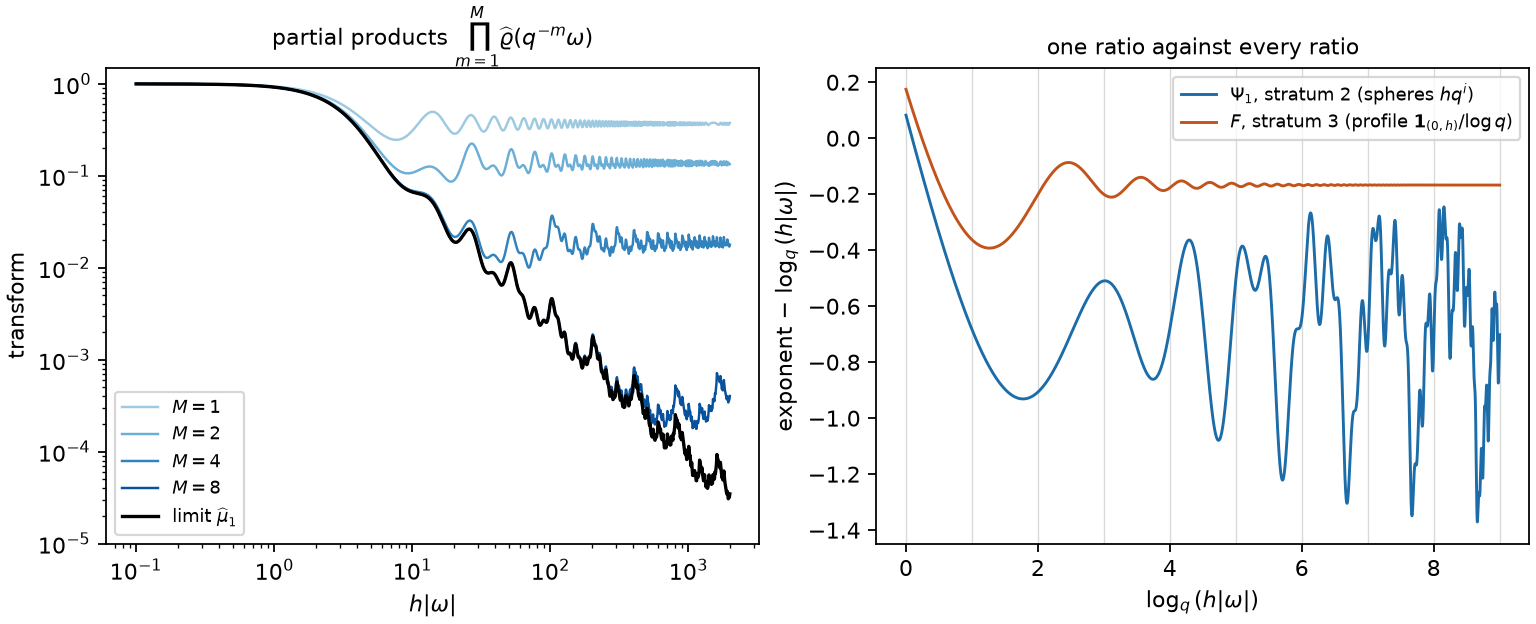
\includegraphics[width=\textwidth]{theory-strata.png}
\caption{The family of Proposition~\ref{prop:stratum-two-example} at $d = 2$, $q = 2$, $h = 1$,
with the weights $w_i = 1$ for $i < 0$ and $w_i = 0$ for $i \ge 0$ of the proof of
Theorem~\ref{thm:lattice-strata-strict}. Its ladder step $\varrho = \mu_{1,q}$ has the \Levy{}
measure $\sigma_h$, so $\widehat\varrho(\omega) = \exp\bigl(-(1 - J_0(h|\omega|))\bigr)$, where
$J_0 = \Omega_2$ is the Bessel function of order $0$. Left: the partial products of
Proposition~\ref{prop:ladder-knot-kernel}(1) for $M = 1, 2, 4, 8$, and their limit
$\widehat\mu_1$. At high frequency each factor tends to $e^{-1}$, so the $M$-th partial product
levels off near $e^{-M}$. Right, blue: $P(\omega) := \Psi_1(\omega) - \log_q(h|\omega|)$, with
$\Psi_1$ the exponent of the knot kernel. It satisfies $P(q\omega) - P(\omega) = -J_0(h|\omega|)$.
Since $|J_0(x)| \le Cx^{-1/2}$, these differences are summable along each ray $q^n\omega$, so $P$
converges to a function of period $1$ in $\log_q(h|\omega|)$. That this limit is not constant is
read from the plot. Orange: the same difference for the exponent $F(|\omega|)$ of the isotropic
origin datum $(0, (\log q)^{-1}\mathbf 1_{(0,h)})$, which spreads the same jumps evenly in $\log$
length. It lies in $\mathcal{A}_2$ (Theorem~\ref{thm:cited-A35}), and its difference tends to a
constant. The blue sum is cut at $m \le 89$. The orange integral is a trapezoid rule on
$4 \times 10^6$ steps of $[0, 1.001\,r_{\max}]$, with $r_{\max} = h q^9$ the largest frequency
plotted. The script \texttt{scripts/make\_figures\_theory.py} draws the figure.}
\label{fig:theory-strata}
\end{figure}

In clause (3), ``almost every $\omega$'' cannot be replaced by ``every $\omega \ne 0$'', as the next
example shows.

% shared with blueprint prop:ladder-not-every-frequency
\begin{proposition}[the partial products at one frequency]
\label{prop:ladder-not-every-frequency}

Let $d = 1$ and $q = 2$, and let $\varrho$ be the compound Poisson law on $\ZZ$ with the \Levy{}
measure $\nu_\varrho := \sum_{j \ge 1}j^{-2}\cdot\tfrac12(\delta_{2^j} + \delta_{-2^j})$, whose folded
\Levy{} measure is $\sum_{j \ge 1}j^{-2}\delta_{2^j}$. Then $\int\log_+|x|\,\nu_\varrho(dx) = \infty$,
and the partial products $\prod_{m=1}^M\widehat\varrho(2^{-m}\omega)$ have a positive limit at
$\omega = 2\pi$.
\end{proposition}

\begin{proof}
The measure $\nu_\varrho$ is symmetric with total mass $c := \sum_jj^{-2} < \infty$. Let
$\varrho := e^{-c}\sum_{n \ge 0}\nu_\varrho^{*n}/n!$, the law of $Y_1 + \dots + Y_N$ with $N$ Poisson
of mean $c$ and $Y_1, Y_2, \dots$ independent with law $\nu_\varrho/c$, independent of $N$. It is a
probability law with $\widehat\varrho = e^{-c}\exp\widehat{\nu_\varrho}$, and since $\nu_\varrho$ is
symmetric, $\widehat{\nu_\varrho}(\omega) = \int\cos\omega x\,\nu_\varrho(dx)$, so
$\widehat\varrho(\omega) = \exp\bigl(-\int(1 - \cos\omega x)\,\nu_\varrho(dx)\bigr)
= \exp\bigl(-\sum_jj^{-2}(1 - \cos(2^j\omega))\bigr)$. A law with this transform is $\varrho$, the
transform determining the law. It is carried by $\ZZ$: so is $\nu_\varrho$, and a convolution of two
measures carried by $\ZZ$ is carried by $\ZZ$, so every $\nu_\varrho^{*n}$ is. It is infinitely
divisible: for $n \ge 1$ the compound Poisson law of $\nu_\varrho/n$ has the transform
$\widehat\varrho^{1/n}$, so its $n$-th convolution power is $\varrho$. The moment fails:
$\int\log_+|x|\,\nu_\varrho(dx) = \sum_jj^{-2}\cdot j\log 2 = \infty$, the harmonic series diverging.
At $\omega = 2\pi$,
\[
  -\log\prod_{m=1}^M\widehat\varrho(2^{-m}\cdot2\pi) = \sum_{m=1}^M\sum_{j \ge 1}j^{-2}\bigl(1 - \cos(2\pi2^{j-m})\bigr).
\]
The terms with $m \le j$ vanish, since $2^{j-m}$ is an integer. Writing $i := m - j \ge 1$ for the
others, the double sum increases with $M$ to
\[
  \sum_{m \ge 1}\sum_{j \ge 1}j^{-2}\bigl(1 - \cos(2\pi2^{j-m})\bigr) = \Bigl(\sum_{j \ge 1}j^{-2}\Bigr)
  \sum_{i \ge 1}\bigl(1 - \cos(2\pi2^{-i})\bigr) < \infty,
\]
since $1 - \cos u \le u^2/2$ makes the last series at most $\sum_i2\pi^24^{-i}$. (The sums are of
nonnegative terms, so they may be taken over $m$ for each $j$ first.) So the partial products at
$2\pi$ decrease to the positive limit $\exp\bigl(-\sum_m\sum_jj^{-2}(1 - \cos(2\pi2^{j-m}))\bigr)$.

Every step is machine-checked, with no cited fact.
\end{proof}

In sum, the ladder fixes the knot kernels, and the families through one ladder differ only between
the knots. A symmetric infinitely divisible law other than a point mass is the step $\mu_{1,q}$ of a
symmetric $q$-covariant family in the canonical discrete gauge exactly when it has the logarithmic
moment (clauses (1) and (2)). This sorts the masks of grid pyramids. A symmetric infinitely
divisible mask $\varrho \ne \delta_0$ on a full-rank lattice with the moment is the step of a
pyramid strictly in stratum~2, and of no family in stratum~3 (clause (4)(a)). A finite mask other
than a point mass is the step of no family at all, as the next subsection shows.

\subsection{Steps of bounded support}
\label{sec:pyramid-bounded}

This last subsection returns to the classical pyramids. They smooth with a finite mask, applied
separably [\sscite{burt1983laplacian}, p.~533]. The mask is a five-tap mask of Burt's family or a
B-spline mask. The binomial $\tfrac1{16}[1,4,6,4,1]$ is in Burt's family
[\sscite{burt1981fast}, p.~24]. No such mask is a step of any family that is continuous in scale,
whatever its symmetry or covariance. The proposition joins two facts of probability theory: the
increments of an additive process in law are infinitely divisible [\sscite{sato1999levy},
Thm.~9.1, p.~47], and an infinitely divisible law other than a point mass has unbounded support
(Theorem~\ref{thm:cited-A46}).

% shared with blueprint prop:no-bounded-step
\begin{proposition}[no continuous family has a step of bounded support]
\label{prop:no-bounded-step}

Let $w$ be a probability measure on $\RR^d$ with bounded support, not a point mass. Then $w$ is not
infinitely divisible. So $w$ is no $\mu_{s,t}$ of any family of probability measures on $\RR^d$ with
(I1) and (I2), with no assumption of symmetry, rotation invariance, covariance or (ND).
\end{proposition}

\begin{proof}
By Theorem~\ref{thm:cited-A46}, an infinitely divisible law on $\RR^d$ that is not a point mass
has unbounded support. This is the first sentence. For the second, let $(\mu_{s,t})$ satisfy (I1)
and (I2). By Lemma~\ref{lem:steps-infinitely-divisible} every $\mu_{s,t}$ is infinitely
divisible. So $w$, which is not, is no $\mu_{s,t}$.

Every step is machine-checked, and the cited facts are \ledger{A46} and, through
Lemma~\ref{lem:steps-infinitely-divisible}, \ledger{A41}.
\end{proof}

This excludes the binomial mask, its tensor powers and the B-spline masks, on the continuum and on
any grid. The exclusion rests on continuity in scale. If only the levels are looked at, a finite
mask can behave like a step. A law $\mu$ is \emph{refinable} if it satisfies the \emph{knot
relation} $D_q\mu = \mu * w$ for some law $w$, the mask. Its dilate is then the law itself smoothed
by $w$, which is what a step does to a knot kernel. The word is that of subdivision, where a
function $\phi$ with $\phi(x) = \sum_k a_k\phi(2x - k)$ is called refinable
[\sscite{cavaretta1991stationary}, (1.7), pp.~4--5].
On the line the knot relation says that $X$ and $q^{-1}X + q^{-1}Y$ have one law, with $Y$ of law $w$
independent of $X$. By Vervaat's theorem on this equation a solution exists exactly when
$E\log_+|Y| < \infty$ [\sscite{vervaat1979stochastic}, Thm.~1.6(b), p.~757]. So a mask on the line
has a refinable law exactly when it has a logarithmic moment, whether or not it is infinitely
divisible.
Clause (2) of the next proposition shows that the binomial mask has a refinable law, the cubic
B-spline. The convergence belongs to subdivision theory. The scheme of a nonnegative mask converges
under the support condition of [\sscite{cavaretta1991stationary}, Thm.~3.3, p.~48], which the
B-spline masks meet, and the B-splines satisfy the refinement equation of their masks
[\sscite{cavaretta1991stationary}, p.~161]. Clause (2) proves the case at
hand by Vi\`ete's product and reads the limit as a refinable law, a solution of the knot relation
that is the knot kernel of no family. Clause (1) reads Burt's observation that the rescaled equivalent weights approach one
shape [\sscite{burt1981fast}, Obs.~1, p.~24]. The shape is approached and never reached, since no
equivalent weight is the $q$-dilate of the one before. That clause holds for every $q > 0$, though
a pyramid has $q > 1$.

% shared with blueprint prop:equivalent-weights
\begin{proposition}[equivalent weights and the knot relation]
\label{prop:equivalent-weights}

Let $w$ be a law on $\RR^d$, $q > 0$, and $W_n := w * D_qw * \dots * D_{q^{n-1}}w$ the equivalent
weight at level $n$, with $W_0 := \delta_0$.
\begin{enumerate}
\item If $w \ne \delta_0$, then $W_n \ne D_qW_{n-1}$ for every $n \ge 1$: no equivalent weight is the
$q$-dilate of the one before it, for any mask, symmetric or not, infinitely divisible or not.
\item A finite mask can satisfy the knot relation. For instance, let $q = 2$ and let $w$ be the
binomial mask on $h\ZZ$,
\[
  w = \tfrac1{16}\bigl(\delta_{-2h} + 4\delta_{-h} + 6\delta_0 + 4\delta_h + \delta_{2h}\bigr).
\]
The law $\mu_1$ with
$\widehat\mu_1(\omega) = \prod_{m \ge 1}\widehat w(2^{-m}\omega) = \bigl(\sin(h\omega/2)/(h\omega/2)\bigr)^4$,
the cubic B-spline, has $D_2\mu_1 = \mu_1 * w$, and its tensor powers do the same on $h\ZZ^d$.
\end{enumerate}
\end{proposition}

\begin{proof}
(1) Write $P(\omega) := \widehat W_{n-1}(q\omega) = \prod_{k=1}^{n-1}\widehat w(q^k\omega)$, the
transform of $D_qW_{n-1}$. Since $W_n = w * D_qW_{n-1}$, the equation $W_n = D_qW_{n-1}$ would give
$\widehat w\,P = P$, that is $(1 - \widehat w)P = 0$. The function $P$ is continuous with
$P(0) = 1$, so it has no zero on a ball $B_\eta$ about $0$, and $\widehat w = 1$ on $B_\eta$.

A probability measure $w$ with $\widehat w = 1$ on $B_\eta$ is $\delta_0$. Indeed, if
$\widehat w(\omega) = 1$, then $\int(1 - \cos\langle\omega, x\rangle)\,w(dx) = 0$, and the integrand
is nonnegative, so $\cos\langle\omega, x\rangle = 1$ for $w$-almost every $x$. Let $b_1, \dots, b_d$
be a basis and $c > 0$ with $c|b_j| < \eta$ for every $j$. Applying this at the countably many points
$c\,b_j/m$, $m \ge 1$, gives a $w$-null set off which $\cos(c\langle b_j, x\rangle/m) = 1$ for every
$j$ and every $m$. A real number $\theta$ with $\cos(\theta/m) = 1$ for every $m \ge 1$ is $0$,
since $|\theta/m| < 2\pi$ for $m$ large. So $\langle b_j, x\rangle = 0$ for every $j$, that is $x = 0$,
for $w$-almost every $x$, and $w = \delta_0$. This contradicts $w \ne \delta_0$. At $n = 1$ the
product $P$ is empty and equals $1$.

(2) The transform of the mask is
$\widehat w(\omega) = \tfrac1{16}(e^{-ih\omega/2} + e^{ih\omega/2})^4 = \cos^4(h\omega/2)$. Write
$\operatorname{sinc} x := \sin x/x$, with $\operatorname{sinc} 0 := 1$. Since
$\sin 2t = 2\sin t\cos t$, $\operatorname{sinc}(2t) = \operatorname{sinc}(t)\cos t$, and induction
on $M$ gives
\[
  \operatorname{sinc} x = \operatorname{sinc}(x2^{-M})\prod_{m=1}^{M}\cos(x2^{-m}) .
\]
As $\operatorname{sinc}$ is continuous with $\operatorname{sinc} 0 = 1$, the partial products tend
to $\operatorname{sinc} x$. At $x = h\omega/2$ this gives
$\prod_{m \ge 1}\widehat w(2^{-m}\omega) = (\sin(h\omega/2)/(h\omega/2))^4$. The uniform law on
$[-h/2, h/2]$ has the transform $\operatorname{sinc}(h\omega/2)$, so its fourfold convolution, the
cubic B-spline, has the transform of $\mu_1$. By the uniqueness of the transform it is the only
probability measure with that transform. Then
$\widehat\mu_1(2\omega) = \operatorname{sinc}(h\omega)^4
= \operatorname{sinc}(h\omega/2)^4\cos^4(h\omega/2) = \widehat\mu_1(\omega)\widehat w(\omega)$,
which is $D_2\mu_1 = \mu_1 * w$. For the tensor powers on $h\ZZ^d$ the transforms are products over
the coordinates, and $D_2$ acts on each factor.

Every step is machine-checked, with no cited fact.
\end{proof}

The cubic B-spline shows why Definition~\ref{def:self-decomposable} requires the residual to be
infinitely divisible. With any residual the class is wider. Maejima and Naito give it Lo\`eve's
name, $b$-decomposable, and note that its laws need not be infinitely divisible
[\sscite{maejima1998semi}, Rem.~3.1, pp.~19--20]. The B-spline is $b$-decomposable with $b = 2$. By
$D_2\mu_1 = \mu_1 * w$ it is the law of $\tfrac12X + Y$, with $X$ of that law and $Y$ of the law
$D_{1/2}w$, independent of $X$. Definition~\ref{def:self-decomposable} excludes it. The B-spline has bounded support and is
not a point mass, so it is not infinitely divisible (Proposition~\ref{prop:no-bounded-step}), while
a semi-selfdecomposable law is (Theorem~\ref{thm:cited-A43}). Section~\ref{sec:price-masks} reads
the same example on a grid, after Proposition~\ref{prop:exact-masks}.


% Transcribed from blueprint/src/parts/02-line.tex.
\section{The line and its grids}
\label{sec:line-theory}

Images live in the plane, and Section~\ref{ch:price} builds an exact pyramid on the grid
$h\ZZ^d$. Its mask, the frame mask, is a product of masks on the line, one sampled Laplace mask
along each coordinate axis. This section supplies that mask. It computes the mask's \Levy{} measure,
and it shows that the mask is applied by one forward and one backward recursion.

The line is also where the criterion for an exact pyramid, in the sense of the introduction, can be
read in the weights of a mask. Section~\ref{ch:price} proves the criterion in every dimension, and
its case $d = 1$ is stated here. A symmetric probability mask other than $\delta_0$ on a grid of the line has an
exact pyramid exactly when it is infinitely divisible with a logarithmic moment. The families through
such a pyramid lie in stratum~2 and never in stratum~3.

The line is the case $d = 1$ of Section~\ref{ch:pyramid}, and this section uses that section's
results throughout. The line also has axioms of its own, stated for operators $\Phi_{s,t}$ on
$L^1(\RR)$ as (A1)--(A8) and (ND) of Definition~\ref{def:cascade-measurement-family}. Of these, the
covariance axiom (A8) requires covariance under every dilation. A pyramid needs it only at the
dilations $q^n$, $n \in \ZZ$, which form the closed subgroup $q^{\ZZ}$ of $(0,\infty)$. So this
section requires (A8) at those dilations alone. Read through the kernels, these operator axioms are
those of Section~\ref{ch:pyramid} at $d = 1$, and the first subsection proves it. The three
subsections take these points in turn.
\begin{itemize}
\item Section~\ref{subsec:line-strata} reads the operator axioms through their kernels, so that the
statements of Section~\ref{ch:pyramid} hold at $d = 1$. It then places the families of the line
among the three strata.
\item Section~\ref{subsec:grid-pyramids-line} says which masks on a grid have an exact pyramid, and
in which stratum the families through such a pyramid lie.
\item Section~\ref{subsec:sampled-laplace} computes with the sampled Laplace kernels on the grid. It
compares the \Matern{} pyramid, computed by recursion and decimation, with the samples of its
steps.
\end{itemize}
The rest of the theory on the line is in the supplement.

\subsection{The three strata}
\label{subsec:line-strata}

Section~\ref{ch:pyramid} speaks of families of laws, and the axioms of the line speak of operators.
This subsection shows that the two describe the same families, so that every statement of
Section~\ref{ch:pyramid} applies on the line. It then describes the strata in the line's \Levy{}
coordinates, names the knots, and ends with the pyramid principle, which says what covariance means
for sampled kernels.

A statement in $\RR^d$ is read at $d = 1$ through the identification $x \mapsto xe_1$ of $\RR$ with
$\RR^1$. This identification preserves transforms, convolution and dilations. It also preserves
symmetry, infinite divisibility, lattices, the absolute value and Lebesgue measure.

The first definition fixes the operator families of a pyramid on the line. They satisfy (A1)--(A7)
and (ND), and (A8) is required of them at the dilations in $q^{\ZZ}$ only.

% shared with blueprint def:q-covariant-line
\begin{definition}[families on the line covariant under one ratio]
\label{def:q-covariant-line}

Let $q > 1$. A family $(\Phi_{s,t})_{0 \le s \le t}$ of linear operators on $L^1(\RR)$ is
\emph{$q^{\ZZ}$-covariant} if it satisfies (A1)--(A7) and (ND) of
Definition~\ref{def:cascade-measurement-family}, and (A8) required at the dilations in $q^{\ZZ}$:
there are increasing bijections $S_\lambda$ of $[0,\infty)$, $\lambda \in q^{\ZZ}$, with
$\mathcal{D}_\lambda\Phi_{s,t} = \Phi_{S_\lambda s, S_\lambda t}\mathcal{D}_\lambda$ for all
$s \le t$. This condition is written (A8$|q^{\ZZ}$). The family is in the \emph{canonical
discrete gauge} if $S_qt = qt$ for all $t$. It is \emph{fully covariant} if it satisfies
(A1)--(A8) and (ND).
\end{definition}

The next lemma passes between operators and their kernels. Its last sentence is what the rest of the
section uses: a $q^{\ZZ}$-covariant family is, through its kernels, a symmetric $q$-covariant family
in dimension $1$ in the sense of Section~\ref{ch:pyramid}.

% shared with blueprint lem:line-axioms-kernels
\begin{lemma}[the axioms on the line, read on the kernels]
\label{lem:line-axioms-kernels}

Let $(\Phi_{s,t})_{0 \le s \le t}$ be linear operators on $L^1(\RR)$.
\begin{enumerate}
\item If they satisfy (A1)--(A7), then $\Phi_{s,t}f = \mu_{s,t} * f$ for a unique family of
symmetric probability measures $\mu_{s,t}$ on $\RR$, the \emph{kernels}. These satisfy (I1) and
(I2), and (ND) holds if and only if $\mu_{s,t} \ne \delta_0$ for $s < t$. So the kernels of a
family with (A1)--(A7) and (ND) are a symmetric family in dimension $1$
(Definition~\ref{def:family-dimension-d}).
\item Conversely, if symmetric probability measures $\mu_{s,t}$ on $\RR$ satisfy (I1) and (I2),
the operators $\Phi_{s,t}f := \mu_{s,t} * f$ satisfy (A1)--(A7), and they satisfy (ND) if and
only if $\mu_{s,t} \ne \delta_0$ for $s < t$. In particular a symmetric family in dimension $1$
gives a family with (A1)--(A7) and (ND).
\item Let $\lambda > 0$ and let $S$ be an increasing bijection of $[0,\infty)$. Then
$\mathcal{D}_\lambda\Phi_{s,t} = \Phi_{Ss,St}\mathcal{D}_\lambda$ for all $s \le t$ if and only
if $T_\lambda\mu_{s,t} = \mu_{Ss,St}$ for all $s \le t$. So (A8) at the dilation $\lambda$ is
$\lambda$-covariance of the kernels, with the same bijection.
\end{enumerate}
So the $q^{\ZZ}$-covariant families (Definition~\ref{def:q-covariant-line}) are, read through their
kernels, the symmetric $q$-covariant families in dimension $1$, with the same bijections.
\end{lemma}

\begin{proof}
Write $g(x) := (2\pi)^{-1/2}e^{-x^2/2}$, whose transform $\widehat g(\omega) = e^{-\omega^2/2}$
has no zero. For a finite measure $\mu$ the transform of $\mu * g$ is $\widehat\mu\,\widehat g$,
so the operator $f \mapsto \mu * f$ determines $\widehat\mu$, hence $\mu$.

(1) By Theorem~\ref{thm:cited-A1}, under (A1), (A2), (A4) and (A5) each
$\Phi_{s,t}$ is the convolution with a unique probability measure $\mu_{s,t}$, which is
symmetric under (A3). (A6) reads $\delta_0 * f = \mu_{t,t} * f$ and
$(\mu_{s,t} * \mu_{r,s}) * f = \mu_{r,t} * f$ for every $f \in L^1$, by the associativity of
convolution. By the remark above this is $\mu_{t,t} = \delta_0$ and
$\mu_{r,t} = \mu_{s,t} * \mu_{r,s}$, which is (I1). For (I2) let $(s_n,t_n) \to (s,t)$ in
$\{0 \le s \le t\}$. Since the transform of an integrable function is bounded by its $L^1$ norm,
\[
  \bigl|\widehat\mu_{s_n,t_n}(\omega) - \widehat\mu_{s,t}(\omega)\bigr|\,\widehat g(\omega)
  \le \bigl\|\mu_{s_n,t_n} * g - \mu_{s,t} * g\bigr\|_1 ,
\]
and the right side tends to $0$ by (A7). Since $\widehat g(\omega) > 0$, this is (I2). Finally
$\Phi_{s,t} = \mathrm{Id}$ if and only if $\mu_{s,t} = \delta_0$, by the remark above.

(2) The converse half of Theorem~\ref{thm:cited-A1} gives (A1)--(A5). (A6) is (I1) and the
associativity of convolution, and $\Phi_{s,t} \ne \mathrm{Id}$ if and only if
$\mu_{s,t} \ne \delta_0$, by the remark above. For (A7) write $\tau_yf := f(\cdot - y)$ and
$\Theta_f(y) := \|\tau_yf - f\|_1$, a bounded continuous function with $\Theta_f(0) = 0$, by the
continuity of translation in $L^1$. For a probability $\nu$, $\nu * f - f$ is the
$\nu$-average of $\tau_yf - f$, so $\|\nu * f - f\|_1 \le \int\Theta_f\,d\nu$. Let
$(s_n,t_n) \to (s,t)$ and move one endpoint at a time,
through $(s_n, t)$ when $s_n \le t$, and through $(s, t_n)$ otherwise, where
$s \le t < s_n \le t_n$. By (I1),
$\mu_{s,t} * f - \mu_{s',t} * f = \mu_{s'',t} * (\mu_{u,v} * f - f)$ up to sign, with
$u = \min(s, s')$, $v = \max(s, s')$ and $s''$ the larger of the two, so
$\|\mu_{s,t} * f - \mu_{s',t} * f\|_1 \le \|\mu_{u,v} * f - f\|_1 \le \int\Theta_f\,d\mu_{u,v}$,
convolution with a probability being a contraction of $L^1$. In the same way
$\|\mu_{s,t} * f - \mu_{s,t'} * f\|_1 \le \int\Theta_g\,d\mu_{\min(t,t'),\max(t,t')}$ with $g$ the
convolution of $f$ with the earlier factor, and $\Theta_g \le \Theta_f$ since translation commutes
with convolution. As the two ends of an increment tend to a common limit $c$, its transform tends
to $\widehat\mu_{c,c} = 1$ by (I2), so the increment tends weakly to $\delta_0$ by \Levy's
continuity theorem, and $\int\Theta_f$ against it tends to $\Theta_f(0) = 0$. This gives (A7).

(3) For a probability $\mu$ and $f \in L^1$,
\[
  (T_\lambda\mu) * (\mathcal{D}_\lambda f)(x) = \int\lambda^{-1}f\bigl((x - \lambda y)/\lambda\bigr)\,\mu(dy)
  = \lambda^{-1}(\mu * f)(x/\lambda) = \mathcal{D}_\lambda(\mu * f)(x) .
\]
So $\mathcal{D}_\lambda\Phi_{s,t}f = (T_\lambda\mu_{s,t}) * \mathcal{D}_\lambda f$, while
$\Phi_{Ss,St}\mathcal{D}_\lambda f = \mu_{Ss,St} * \mathcal{D}_\lambda f$. Since
$\mathcal{D}_\lambda$ maps $L^1$ onto $L^1$, the two operators agree for every $f$ if and only if
the convolutions with $T_\lambda\mu_{s,t}$ and with $\mu_{Ss,St}$ agree on all of $L^1$, that is,
by the remark above, if and only if $T_\lambda\mu_{s,t} = \mu_{Ss,St}$.

For the last sentence, by (1)--(3) a family with (A1)--(A7), (ND) and (A8) at every
$\lambda \in q^{\ZZ}$ is, through its kernels, a symmetric family in dimension $1$ that is
$\lambda$-covariant at every $\lambda \in q^{\ZZ}$, with the same bijections, and conversely. In
particular it is $q$-covariant. Conversely a $q$-covariant symmetric family is
$\lambda$-covariant at every $\lambda \in q^{\ZZ}$, since the set of $\lambda$ at which it is
covariant is a group, with $S_{q^n} = S_q^n$ (Lemma~\ref{lem:family-dilations}(1)--(2)):
covariance at $\lambda$ with $S$ and at $\lambda'$ with $S'$ gives covariance at $\lambda\lambda'$
with $S \circ S'$, and at $\lambda^{-1}$ with $S^{-1}$, so $S_q$ iterated $n$ times serves $q^n$,
and its inverse iterated serves $q^{-n}$.

Every step is machine-checked, Theorem~\ref{thm:cited-A1} included.
\end{proof}

The strata of Section~\ref{ch:pyramid} are described by \Levy{} data, and on the line these data
take a simpler form. A symmetric measure on $\RR$ is determined by its image under
$x \mapsto |x|$, its \emph{fold}. So the line's statements carry a symmetric \Levy{} measure as a
measure on $(0,\infty)$, which gives the rate of the jumps of each length. The next definition names
the pair this gives.

% shared with blueprint def:folded-data
\begin{definition}[folded data]
\label{def:folded-data}

For a symmetric infinitely divisible law on $\RR$ with exponent
$\Psi(\omega) = a\omega^2 + \int_{(0,\infty)}(1 - \cos\omega v)\,\varpi(dv)$, the pair
$(a, \varpi)$ is its \emph{folded data}: $a$ is the Gaussian coefficient and $\varpi$ the image
of the \Levy{} measure under $x \mapsto |x|$.
\end{definition}

\paragraph{The strata on the line.} One fact is special to the line. Since
$\Orth(1) = \{\pm1\}$, a symmetric family on the line is isotropic. So through
Lemma~\ref{lem:line-axioms-kernels} the statements of Section~\ref{ch:pyramid} hold on the line at
$d = 1$, those about isotropic families included. The three nested strata of
Section~\ref{sec:pyramid-strata} are among them.

Covariance behaves on the line as in $\RR^d$. The dilations of a family form $\{1\}$, some
$q^{\ZZ}$ or $(0,\infty)$ (Lemma~\ref{lem:family-dilations}(2)). Under covariance at $q$ a
relabelling of the scales gives the canonical discrete gauge $S_qt = qt$
(Lemma~\ref{lem:family-dilations}(4)). Under $q^{\ZZ}$ the gauge is unique only up to the group
$\mathcal{G}_q$ of Lemma~\ref{lem:gauge-group}.

In folded data, covariance and the strata take a concrete form. Write $(a(t), \varpi_t)$ for the
folded data of the kernel $\mu_{0,t}$. The family is $q$-covariant with $S_qt = qt$ if and only if
$a(qt) = q^2a(t)$ and $\varpi_{qt} = T_q\varpi_t$ for all $t > 0$. Every kernel is then
semi-selfdecomposable with span $q$, and the kernels at the scales in $[1, q)$ determine the family
(Lemma~\ref{lem:discrete-covariance-levy}).

Semi-selfdecomposability is meant in the sense of Maejima and Naito [\sscite{maejima1998semi}]
(Definition~\ref{def:self-decomposable}). On the line a symmetric law $\mu$ is
semi-selfdecomposable with span $q > 1$ when
$\widehat\mu(\omega) = \widehat\mu(\omega/q)\,\widehat\varrho_q(\omega)$ for some infinitely
divisible law $\varrho_q$, the residual (Definition~\ref{def:self-decomposable} at $d = 1$). Sato's
criteria for semi-selfdecomposability are recalled in Section~\ref{sec:pyramid-strata}, and folded
data give a short test. For a symmetric law with folded data $(a, \varpi)$ the criterion
$T_q\nu \ge \nu$ of Theorem~\ref{thm:cited-A44} reads $T_q\varpi \ge \varpi$. This holds because
folding commutes with $T_q$ and a symmetric measure is determined by its fold.

Theorem~\ref{thm:lattice-strata} gives the three strata in these coordinates. Its clause (3), read
through Theorem~\ref{thm:cited-A4}, describes stratum~3. A fully covariant family, relabelled by
its gauge, has $a(t) = \alpha t^2$ and $\varpi_t(dv) = k(v/t)\,v^{-1}dv$, with $(\alpha, k)$ the
data of an admissible exponent.

The examples of Section~\ref{sec:pyramid-strata} separate the strata on the line too. At $d = 1$
the uniform law on the sphere of radius $h$ is $\tfrac12(\delta_h + \delta_{-h})$. The family of
Proposition~\ref{prop:stratum-one-example} is then Lindeberg's discrete scale space
[\sscite{lindeberg1990scalespace}], with $\varpi_t = t\,\delta_h$. It is in the first stratum and
not in the second. The family of Proposition~\ref{prop:stratum-two-example} is the
\emph{geometric-jump pyramid}, whose jumps have the lengths $hq^i$, $i \in \ZZ$. It is in the second
stratum and not in the third. With these witnesses
Theorem~\ref{thm:lattice-strata-strict} separates the strata on the line. No kernel $\mu_{0,t}$,
$t > 0$, of a $q^{\ZZ}$-covariant family is carried by a lattice $\xi\ZZ$
(Proposition~\ref{prop:no-lattice-kernel}).

Section~\ref{supp:strata} of the supplement states and proves these statements in the line's own
terms, the operator axioms and the folded data. The counterparts are the following.
\begin{itemize}
\item Lemma~\ref{lem:family-dilations}(2): Lemma~\ref{lem:closed-subgroups}.
\item Lemma~\ref{lem:discrete-covariance-levy}: Lemma~\ref{lem:discrete-covariance-line}.
\item Theorem~\ref{thm:lattice-strata}: Theorem~\ref{thm:lattice-line}.
\item Proposition~\ref{prop:stratum-one-example}: Proposition~\ref{prop:lindeberg-stratum-one}.
\item Proposition~\ref{prop:stratum-two-example}: Proposition~\ref{prop:discrete-gaussian-pyramid}.
\item Theorem~\ref{thm:lattice-strata-strict}: Theorem~\ref{cor:lattice-line-strict}.
\item Proposition~\ref{prop:no-lattice-kernel}: Proposition~\ref{prop:no-lattice-kernel-line}.
\end{itemize}

\paragraph{Knots.} A pyramid stores its levels at the knots, and the grid pyramids below are read
there. The knots, the knot kernels and the ladder of a $q^{\ZZ}$-covariant family in the canonical
discrete gauge are those of its kernels (Lemma~\ref{lem:line-axioms-kernels}), in the sense of
Definition~\ref{def:knots-and-ladder} at $d = 1$. The knots are the scales $q^n$, $n \in \ZZ$, the
ends of the annuli $[q^n, q^{n+1}]$. With the exponents $\Psi_t := -\log\widehat\mu_{0,t}$ of
Lemma~\ref{lem:family-structure}, the knot kernels $\mu_{0,q^n}$ have
$\Psi_{q^n} = \Psi_1(q^n\,\cdot)$ (Lemma~\ref{lem:discrete-covariance-levy}). So they are the
dilates of the one knot kernel $\mu_{0,1}$. Which scale is called $1$ is a choice of gauge
(Lemma~\ref{lem:gauge-group}), and the statements below fix it.

\paragraph{The pyramid principle.} An implemented pyramid works with arrays on grids, so the next
question is what covariance says about them. A step $\mu_{s,t}$ with $s > 0$, unlike a kernel, can
be a lattice law, and a grid pyramid applies such steps. The kernels themselves are carried by no
lattice (Proposition~\ref{prop:no-lattice-kernel}). Where they have continuous densities, an
implemented pyramid can sample them on grids. For an integer $q$ the knot kernels of an exact grid
pyramid have none: they are singular (Proposition~\ref{prop:grid-pyramid-singular-kernels}).
What covariance says about the samples, where they exist, is the pyramid principle of
Section~\ref{ch:pyramid} at $d = 1$, Proposition~\ref{prop:no-lattice-kernel-line}(2). In the canonical discrete gauge, if $\mu_{0,t}$
has a continuous density $\phi_t$ for some $t > 0$, then $q^n\phi_{q^nt}(q^nhm) = \phi_t(hm)$ for
all $n \in \ZZ$, $h > 0$ and $m \in \ZZ$. Sampled at the scale $q^nt$ on the grid $q^nh\ZZ$, the
kernel is the same array at every level, up to the factor $q^n$.
Figure~\ref{fig:pyramid-schematic} shows the knots, the grids and the one mask applied at every
level.

\subsection{Grid pyramids: which masks have a pyramid, and in which stratum}
\label{subsec:grid-pyramids-line}

A pyramid of the literature is given by its mask, an array of positive weights on a grid. The
question for such a pyramid is whether some family of the axioms has the mask, dilated to each
level, as its ladder. Section~\ref{ch:pyramid} answered it for laws in $\RR^d$, lattice laws
included. A symmetric law other than $\delta_0$ is the octave step $\mu_{1,q}$ of a symmetric
$q$-covariant family in the canonical discrete gauge exactly when it is infinitely divisible with a
logarithmic moment (Proposition~\ref{prop:ladder-knot-kernel}). This subsection reads that answer
for masks on a grid of the line, in the operator axioms. The criterion of the next proposition
rests on Proposition~\ref{prop:ladder-knot-kernel} at $d = 1$. The subsection also says in which
stratum the families through such a pyramid lie.

The finite masks of the classical pyramids are already excluded. A law of bounded support other
than a point mass is a step of no family with (I1) and (I2)
(Proposition~\ref{prop:no-bounded-step}). But a mask need not be finite to be implementable. The
sampled Laplace mask has infinitely many nonzero weights, and it is applied by one forward and one
backward recursion (Proposition~\ref{prop:recursion-helmholtz}(2)). So the criterion has to be read
on infinite masks, where it becomes a condition on the weights.

The stratum needs an argument of its own. In the continuum, for steps with a rational transform,
\prog{V-cone v0.1}{Prop.~7.5(2), p.~65} (Theorem~\ref{thm:cited-A20}) decides whether the covariant
interpolant of the step is admissible, the exponent of a fully covariant family. Its criterion is a
condition on the \Levy{} profile: the sum of the dilates of the profile must have a nonincreasing
version. The \Levy{} measure of a lattice mask is atomic, so it has no profile, and this criterion
does not apply to it. Clause (3) of the next proposition settles the question on the lattice
instead. Throughout, $h > 0$ is the grid spacing and $\vartheta = h\omega$ the grid frequency.

% shared with blueprint def:grid-pyramid-line
\begin{definition}[the grid pyramid of a mask]
\label{def:grid-pyramid-line}

Let $q > 1$ and $h > 0$, and let $w \ne \delta_0$ be a symmetric probability law on $h\ZZ$, the
\emph{mask}. The \emph{grid pyramid} of $(w, q)$ is the ladder $\mu_{q^n,q^{n+1}} := T_{q^n}w$,
$n \in \ZZ$, read in the canonical discrete gauge $S_qt = qt$, so that its knots are the scales
$q^n$: the same array, applied on the grid $q^nh\ZZ$ at every level. It is
\emph{exact} if some $q^{\ZZ}$-covariant family in the canonical discrete gauge has these
steps, through its kernels (Lemma~\ref{lem:line-axioms-kernels}), and \emph{exact in the third stratum} if
some such family is fully covariant.
\end{definition}

The definition is the pyramid principle read on the steps rather than on the kernels. Only one step
has to be checked. Under (A8$|q^{\ZZ}$) with $S_qt = qt$ the one requirement $\mu_{1,q} = w$
already forces the ladder, since covariance at $q^n$ gives $T_{q^n}\mu_{1,q} = \mu_{q^n,q^{n+1}}$
(Lemma~\ref{lem:line-axioms-kernels}(3)). So either notion is a condition on one step.

Exactness here is the sense of the introduction. On a grid the word \emph{exact} has three senses,
fixed in Definition~\ref{def:exact-senses} of Section~\ref{ch:price}, and this section uses all
three. A fourth phrase stands apart.
\begin{itemize}
\item A grid computation is exact in sense (i) when the arrays it produces, in exact arithmetic,
equal the kernels they stand for. A continuum kernel stands for its renormalized samples.
\item The subsample of a member of a grid family is exact in sense (ii) when, renormalized to mass
one, it is a member of the same family on the coarser grid.
\item A grid pyramid is exact in sense (iii) when a family continuous in scale and covariant under
$q$ carries its ladder. On the line this is the exactness of the definition above.
\item An \emph{exact cascade on the grid} is a family on one grid whose increments are again grid
kernels. The phrase names none of the three senses.
\end{itemize}
Exactness in the third stratum requires in addition that the carrying family be fully covariant.
Definition~\ref{def:exact-grid-pyramid} states the notion in $\RR^d$, on laws, and this definition
is its operator form on the line. The two agree at $d = 1$
(Proposition~\ref{prop:line-and-arrays}(1)).

The next proposition answers the question of this subsection. A mask has an exact grid pyramid
exactly when it is infinitely divisible and has a logarithmic moment,
$\int\log_+|x|\,w(dx) < \infty$. Since $\log_+x \le x^p/(pe)$ for $x \ge 0$ and $p > 0$, every
mask with a finite moment of some positive order has it. Every family through an exact grid pyramid then lies in stratum~2 and not in stratum~3. Clause (1)
says which masks are infinitely divisible, and clause (4) applies the criterion to the sampled
Laplace mask and to the classical finite masks. For laws the sufficiency is the theorem of Maejima
and Ueda [\sscite{maejima2009stochastic}, Thm.~3.3, p.~353]. The necessity of infinite divisibility
comes from continuity in scale (Lemma~\ref{lem:steps-infinitely-divisible}).

Clause (1) also places the exact masks against Burt's equal contribution. An exact mask has a
positive transform. For an integer ratio $r$, equal contribution requires
$\sum_iw(h(j + ir)) = 1/r$ for every $j$ [\sscite{burt1981fast}, (C4), p.~23], which Burt and
Adelson state for $r = 2$ [\sscite{burt1983laplacian}, p.~533]. In transforms it requires
$\widehat w$ to vanish at the frequencies $2\pi k/(rh)$, $0 < k < r$. So no exact mask has equal
contribution at an integer ratio. Burt motivates the condition by the equal weight of every sample
under reduction and by the convergence of the equivalent kernels [\sscite{burt1981fast}, p.~24].

% shared with blueprint prop:grid-pyramids-infinitely-divisible
\begin{proposition}[grid pyramids and infinitely divisible masks]
\label{prop:grid-pyramids-infinitely-divisible}

Let $q > 1$, $h > 0$, and let $w \ne \delta_0$ be a symmetric probability law on $h\ZZ$.
\begin{enumerate}
\item \emph{(Lattice carrier.)} The mask $w$ is infinitely divisible if and only if it is compound
Poisson,
\[
  \widehat w(\omega) = \exp\Bigl(-\int_{(0,\infty)}(1 - \cos\omega v)\,\varpi_w(dv)\Bigr),
\]
with a finite measure $\varpi_w \ne 0$ carried by $h\ZZ_{>0}$, its folded \Levy{} measure. Then
$\widehat w > 0$ everywhere and the support of $w$ is unbounded. So a mask of bounded support is
not infinitely divisible.
\item \emph{(Criterion, and the covariant kernel.)} The grid pyramid of $(w, q)$ is exact if
and only if
\begin{equation}
\label{eq:grid-pyramid-criterion}
  w \text{ is infinitely divisible and } \int_{(0,\infty)}\log_+v\;\varpi_w(dv) < \infty ,
\end{equation}
equivalently if and only if $w$ is infinitely divisible and $\int\log_+|x|\,w(dx) < \infty$. Its
knot kernel is then unique: every family carrying the ladder has $a(1) = 0$ and
\begin{equation}
\label{eq:grid-pyramid-knot-kernel}
  \varpi_1 = \sum_{m \ge 1}T_{q^{-m}}\varpi_w, \qquad
  \widehat\mu_{0,1}(\omega) = \prod_{m \ge 1}\widehat w(q^{-m}\omega),
\end{equation}
the product being the limit of the transforms of $T_{q^{-1}}w * \dots * T_{q^{-M}}w$ as
$M \to \infty$. The measure $\varpi_1$ is carried by the union of the sets $q^{-m}h\ZZ_{>0}$,
$m \ge 1$, and by no lattice $\xi\ZZ$. When $w$ is infinitely divisible and
$\int\log_+v\;\varpi_w(dv) = \infty$, the partial products
have no limit that is a characteristic function, and they tend to $0$ at almost every $\omega$,
though not in general at every $\omega \ne 0$ (at $q = 2$, by
Proposition~\ref{prop:ladder-not-every-frequency}): there is no kernel. The families carrying the ladder
are not unique. One of them is the \emph{uniform coupling}, with $a(t) = 0$ and
$\varpi_t = \varpi_1 + (\log_qt)\,\varpi_w$ for $t \in [1,q]$, each atom of the mask switched on
linearly in $\log t$ across the octave.
\item \emph{(No grid pyramid is exact in the third stratum.)} For no $q > 1$, $h > 0$ and mask $w$ is the
grid pyramid of $(w, q)$ exact in the third stratum. More generally, a symmetric law $\varrho \ne \delta_0$
carried by a lattice $\xi\ZZ$, $\xi > 0$, is a step $\mu_{s,t}$ of no fully covariant family. So
every family carrying an exact grid pyramid lies in the second stratum of
Theorem~\ref{thm:lattice-line} and not in the third: the pyramid has a covariant kernel, unique at
the knots, and no fully covariant family interpolates its levels.
\item \emph{(Instances.)} For $0 < a < 1$ the \emph{sampled Laplace mask}
$\lambda^{\mathrm{L}}_a$, the law on $h\ZZ$ with $\lambda^{\mathrm{L}}_a(\{hn\}) =
\tfrac{1-a}{1+a}a^{|n|}$, is infinitely divisible, with all moments finite. So the
\emph{geometric pyramid}, the grid pyramid of $(\lambda^{\mathrm{L}}_a, q)$, is exact for
every $q > 1$, with the unique knot kernel
\begin{equation}
\label{eq:geometric-pyramid-knot-kernel}
  \widehat\mu_{0,1}(\omega) = \prod_{m \ge 1}\Bigl[1 + 2\varsigma\bigl(1 - \cos(q^{-m}h\omega)\bigr)\Bigr]^{-1},
  \qquad \varsigma := \frac{a}{(1-a)^2},
\end{equation}
and by (3) it lies in no stratum above the second.
No mask of bounded support has an exact grid pyramid. Among these masks are two families of odd
length: the binomial masks with the weights $4^{-k}\binom{2k}{k+n}$ at $hn$, $|n| \le k$,
$k \ge 1$, which are the refinement masks of the B-splines of odd degree $2k - 1$ and include
$\tfrac1{16}[1,4,6,4,1]$ at $k = 2$, and the sampled B-spline masks, the values $\beta(n)$, $n \in \ZZ$, of a B-spline $\beta$
of degree at least $2$ with unit knot spacing, centred at $0$, placed at $hn$ and renormalized to unit
mass.
\end{enumerate}
\end{proposition}

\begin{proof}
A measure $\varpi$ on $(0,\infty)$ has the symmetrization $\varpi_s$, the symmetric measure on
$\RR$ that puts half of $\varpi$ on each side of $0$. Then $\varpi_s(B) = \tfrac12\varpi(B)$ for
$B \subseteq (0,\infty)$, so a measure on $(0,\infty)$ is determined by its symmetrization, and
symmetrization commutes with sums and with dilations. Since $\cos$ is even,
$\int(1 - \cos\omega x)\,\varpi_s(dx) = \int_{(0,\infty)}(1 - \cos\omega v)\,\varpi(dv)$. So
$(a, \varpi)$ is a folded pair of the exponent of a law $m$ on $\RR$ if and only if $m$ has the
data $(a, \varpi_s)$.

(1) Let $w$ be infinitely divisible, with folded data $(a, \varpi_w)$
(Lemma~\ref{lem:line-exponent-data}(1)). Then $w$, carried by the lattice $h\ZZ$, has the data
$(a, (\varpi_w)_s)$, the generating triplet $(2a, (\varpi_w)_s, 0)$ in Sato's normalization
(Lemma~\ref{lem:symmetric-levy-khintchine}). By
Lemma~\ref{lem:lattice-infinitely-divisible} at $d = 1$, $2a = 0$, and $(\varpi_w)_s$ is finite and
carried by $h\ZZ \setminus \{0\}$. Hence $\varpi_w = 2(\varpi_w)_s$ on $(0,\infty)$ is finite and
carried by $h\ZZ_{>0}$. So $-\log\widehat w(\omega) = \int(1 - \cos\omega v)\,\varpi_w(dv)$, the
display, and $\widehat w > 0$. And $\varpi_w \ne 0$, since otherwise $w = \delta_0$.
Conversely, let $\widehat w$ have this form with $\varpi_w$ finite. Put
$|\varpi_w| := \varpi_w\bigl((0,\infty)\bigr)$ and let $\sigma$ be the symmetric law
$|\varpi_w|^{-1}(\varpi_w)_s$ on $\RR$. Then $\widehat w = e^{|\varpi_w|(\widehat\sigma - 1)}$
is the transform of the compound Poisson law
$\sum_{k \ge 0}e^{-|\varpi_w|}\tfrac{|\varpi_w|^k}{k!}\sigma^{*k}$, and the $n$-th power of
$e^{(|\varpi_w|/n)(\widehat\sigma - 1)}$, a transform of the same kind, for every $n$. So $w$ is
infinitely divisible. The mask, symmetric and other than $\delta_0$, is not a point mass. So by
Proposition~\ref{prop:no-bounded-step} at $d = 1$ an infinitely divisible mask has unbounded
support, and a mask of bounded support is not infinitely divisible.

(2) Suppose the grid pyramid is exact, carried by a $q^{\ZZ}$-covariant family in the
canonical discrete gauge. By Lemma~\ref{lem:line-axioms-kernels} and
Lemma~\ref{lem:discrete-covariance-line} its kernels are a symmetric family in dimension $1$,
$q$-covariant with $S_qt = qt$ and the step $\mu_{1,q} = w$. Its step $w$ is infinitely divisible
(Lemma~\ref{lem:family-structure}), so by (1) $w$ has the data $(0, (\varpi_w)_s)$.
Proposition~\ref{prop:ladder-knot-kernel}(1) at $d = 1$ gives
$\int\log_+|x|\,(\varpi_w)_s(dx) < \infty$, which is $\int\log_+v\;\varpi_w(dv) < \infty$. It
also gives the product formula, $A_1 = A_w/(q^2 - 1) = 0$ and
$\nu_1 = \nu^* = \sum_{m \ge 1}D_{q^{-m}}(\varpi_w)_s$, the symmetrization of
$\varpi_1 = \sum_{m \ge 1}T_{q^{-m}}\varpi_w$. By the first paragraph and the uniqueness of the
folded data (Lemma~\ref{lem:line-exponent-data}(1)), $a(1) = 0$ and $\mu_{0,1}$ has the folded
measure $\varpi_1$. These depend on $w$ only, so the knot kernel is unique. The partial products
are the transforms of the partial convolutions, by $\widehat{T_c m}(\omega) = \widehat m(c\omega)$
and the convolution theorem.

Conversely, let $w$ be infinitely divisible with the moment. By (1), $\varpi_w$ is finite and
nonzero, and $w$ is a symmetric infinitely divisible law on $\RR$, other than $\delta_0$, with the
data $(0, (\varpi_w)_s)$ and $\int\log_+|x|\,(\varpi_w)_s(dx) = \int\log_+v\;\varpi_w(dv) < \infty$.
Proposition~\ref{prop:ladder-knot-kernel}(2) at $d = 1$ gives a symmetric $q$-covariant family in
dimension $1$ with $S_qt = qt$ and the step $\mu_{1,q} = w$. By
Lemma~\ref{lem:line-axioms-kernels}(2) its laws are the kernels of a family with (A1)--(A7) and
(ND), which by Lemma~\ref{lem:discrete-covariance-line} satisfies (A8$|q^{\ZZ}$) in the canonical
discrete gauge. Covariance at $q$, iterated and inverted, gives
$\mu_{q^ns,q^nt} = T_{q^n}\mu_{s,t}$ for every $n \in \ZZ$, so
$\mu_{q^n,q^{n+1}} = T_{q^n}w$: the pyramid is exact. Proposition~\ref{prop:ladder-knot-kernel}(2)
at $d = 1$, applied to $w$, gives two families with the ladder of $w$ that differ at some pair
of scales. The same clause makes the moment of $(\varpi_w)_s$ equivalent to
$\int\log_+|x|\,w(dx) < \infty$.

The measure $\varpi_w \ne 0$ is carried by the countable set $h\ZZ_{>0}$, so it has an atom
$v_0 \in h\ZZ_{>0}$, and $T_{q^{-m}}\varpi_w$ is carried by $q^{-m}h\ZZ_{>0}$. So $\varpi_1$ is
carried by the union of these sets, with the atoms $q^{-m}v_0 \to 0$. A measure carried by $\xi\ZZ$
has no atom in $(0, \xi)$, so $\varpi_1$ is carried by no lattice.

Let $w$ be infinitely divisible without the moment. Then
Proposition~\ref{prop:ladder-knot-kernel}(3) at $d = 1$, applied to $w$, says that the partial
products have no limit that is a characteristic function, and that they tend to $0$ at almost
every $\omega$. No family
carries the ladder, as one would force the moment by the ``only if'' direction above. The partial
products need not tend to $0$ at every $\omega \ne 0$. Take $q = 2$, let $\varrho$ be the law on
$\ZZ$ of Proposition~\ref{prop:ladder-not-every-frequency}, and put
$w := T_h\varrho$. Its transform $\widehat w(\omega) = \widehat\varrho(h\omega)$ has the form of
(1) with the finite measure $\varpi_w = \sum_{j \ge 1}j^{-2}\delta_{h2^j} \ne 0$, so $w$ is
infinitely divisible, symmetric, other than $\delta_0$ and carried by $h\ZZ$. The moment fails:
$\log_+v \le \log_+(hv) + \log_+(1/h)$, so
$\int\log_+(hv)\,\varpi_\varrho(dv) \ge \int\log_+v\;\varpi_\varrho(dv) -
\log_+(1/h)\,\varpi_\varrho\bigl((0,\infty)\bigr) = \infty$, with $\varpi_\varrho = \sum_{j \ge
1}j^{-2}\delta_{2^j}$ of infinite moment by that proposition. The partial products of $w$ at
$\omega = 2\pi/h$ are those of $\varrho$ at $2\pi$, which have a positive limit by that
proposition.

(3) By Lemma~\ref{lem:line-axioms-kernels} the kernels of a fully covariant family form a
symmetric family in dimension $1$ that is $\lambda$-covariant for every $\lambda > 0$, and $\xi\ZZ$
is a full-rank lattice of $\RR$. Proposition~\ref{prop:ladder-knot-kernel}(4)(a) at $d = 1$ is
then the second sentence. It implies
the first, as a grid pyramid exact in the third stratum would have the step $\mu_{1,q} = w$, a law
other than $\delta_0$ carried by $h\ZZ$. A family carrying an exact grid pyramid is in the second
stratum by definition, and by the second sentence it is not fully covariant, its step $w$ being a
lattice law.

(4) The point masses $\tfrac{1-a}{1+a}a^{|n|}$ sum to $1$, since $\sum_na^{|n|} = \tfrac{1+a}{1-a}$.
The transform of $\lambda^{\mathrm{L}}_a$ is the geometric series
$\tfrac{1-a}{1+a}\sum_na^{|n|}e^{inh\omega} = (1-a)^2/(1 - 2a\cos h\omega + a^2)$
(Proposition~\ref{prop:recursion-helmholtz}(2), at the spacing $1$ and the range $t$ with
$e^{-1/t} = a$). Put $z := ae^{i\vartheta}$. Then $1 - 2a\cos\vartheta + a^2 = |1 - z|^2$, and the
series of the logarithm gives
$-\log|1 - z| = \operatorname{Re}\sum_{k \ge 1}z^k/k = \sum_{k \ge 1}\tfrac{a^k}{k}\cos k\vartheta$,
which at $\vartheta = 0$ is $-\log(1 - a)$. Hence
$\log\tfrac{1 - 2a\cos\vartheta + a^2}{(1-a)^2} = \sum_{k \ge 1}\tfrac{2a^k}{k}(1 - \cos k\vartheta)$,
and at $\vartheta = h\omega$
\[
  \widehat{\lambda^{\mathrm{L}}_a}(\omega) = \frac{1-a}{1 - ae^{ih\omega}}\cdot\frac{1-a}{1 - ae^{-ih\omega}}
  = \exp\Bigl(-\sum_{k \ge 1}\frac{2a^k}{k}\bigl(1 - \cos(kh\omega)\bigr)\Bigr) .
\]
So $\lambda^{\mathrm{L}}_a$ has the form of (1) with the finite measure
$\varpi = \sum_{k \ge 1}\tfrac{2a^k}{k}\delta_{kh} \ne 0$ on $h\ZZ_{>0}$; it is therefore symmetric,
other than $\delta_0$, a mask, and infinitely divisible. Its moments are finite for every $p > 0$:
$|hn|^p\tfrac{1-a}{1+a}a^{|n|} \le h^p|n|^Ka^{|n|}$ with $K$ the least integer $\ge p$, and
$\sum_n|n|^Ka^{|n|} < \infty$. As $\log_+x \le x$ for $x \ge 0$, the logarithmic moment is finite,
and (2) applies. As $1 - 2a\cos\vartheta + a^2 = (1-a)^2 + 2a(1 - \cos\vartheta)$, the transform is
$[1 + 2\varsigma(1 - \cos h\omega)]^{-1}$, and the product formula of (2) is the display. Clause
(3) gives the stratum. The binomial mask has the transform $\cos^4(h\omega/2)$, by the binomial
theorem: it is even, so the mask is symmetric, and it vanishes at $\omega = \pi/h$, so the mask is
not $\delta_0$; its support is $\{0, \pm h, \pm2h\}$. A mask of bounded support is not infinitely
divisible by (1), so its grid pyramid is not exact by (2). The binomial masks and the sampled B-spline masks
are masks of bounded support. The binomial weights $4^{-k}\binom{2k}{k+n}$ are symmetric in
$n$, sum to $1$ and are not concentrated at $0$ for $k \ge 1$. A B-spline of degree $r \ge 2$
with unit knot spacing, centred at $0$, is even and positive exactly on $(-(r+1)/2, (r+1)/2)$, so its
values at the integers, placed at $hn$ and renormalized, form a symmetric law with finitely many
atoms, among them $0$ and $\pm h$.

Every step is machine-checked but one: in (4), that the binomial masks other than
$\tfrac1{16}[1,4,6,4,1]$ and the B-spline samples are symmetric masks of bounded support is shown on
paper, in the paragraph above. That a mask of bounded support has no exact grid pyramid is checked
for every such mask.
\end{proof}

The kernel at the knots that clause (2) gives has a classical meaning. It is the equivalent
weighting function of Burt and Adelson [\sscite{burt1983laplacian}, p.~533], run downward in scale:
$T_{q^{-1}}w * \dots * T_{q^{-M}}w$ is the equivalent weight of $M$ levels, rescaled back to the
scale of the step $w$. Its limit is carried by no lattice, as Proposition~\ref{prop:no-lattice-kernel} requires.
Between the knots the ladder leaves a choice. The families that carry it differ in how each atom of
the mask is switched on across one octave. The phase entropy of the supplement, which selects one
such family on some ladders, does not choose here: it is $-\infty$ at every family that carries a
grid pyramid (Proposition~\ref{prop:phase-entropy-ladder-bound}(3)).

Clause (1) has a concrete reading for the sampled Laplace mask. A compound Poisson law
is the law of a sum of independent jumps with a common law, their number being Poisson distributed.
Its rate is the expected number of jumps. The mask $\lambda^{\mathrm{L}}_a$ is compound Poisson
with the rate $\varpi\bigl((0,\infty)\bigr) = \sum_k2a^k/k = 2\log\tfrac{1}{1-a}$. At
$a = e^{-h/t}$ it is the sampled Laplace kernel $\lambda_t$ of range $t$
(Proposition~\ref{prop:recursion-helmholtz}(2)), and the rate is $2\log(t/h) + O(h/t)$. So the
expected number of lattice jumps in one step grows without bound as the grid refines relative to
the scale. The continuum \Matern{} pyramid (Theorem~\ref{thm:matern-pyramid} at $d = 1$) has one
Laplace kernel per octave. On the grid that kernel is a compound Poisson law with this many jumps on
average.

Clause (3) says that the mask is not a step of a fully covariant family. It leaves open whether
the arrays of a grid pyramid are the samples of one. For the sampled Laplace mask and one fully
covariant family, the \Matern{} pyramid, Proposition~\ref{prop:sampled-laplace-exact}(2) answers
this for an integer ratio $q \ge 2$. Sampled on the grids $q^nh\ZZ$, the \Matern{} pyramid has the
sampled Laplace step at every level. From the second level on, the array that these steps compute
is the restriction of a convolution of sampled Laplace kernels. That restriction differs from the
sample of their convolution. So the computed arrays are the samples of the \Matern{} pyramid's
steps at level $1$ and not from level $2$ on. Whether they are the samples of some other fully
covariant family is left open. The computed array is a ladder increment of the geometric pyramid.
At level $n$ it is $\mu_{1,q^n} = T_{q^{n-1}}\lambda^{\mathrm{L}}_a * \dots * T_q\lambda^{\mathrm{L}}_a *
\lambda^{\mathrm{L}}_a$, read on the grid $q^nh\ZZ$ (Proposition~\ref{prop:line-and-arrays}(2)).

\subsection{Grids on the line: the sampled Laplace family}
\label{subsec:sampled-laplace}

The sampled Laplace mask has an exact pyramid
(Proposition~\ref{prop:grid-pyramids-infinitely-divisible}(4)). This subsection asks how it is
applied on a grid, and how what it computes compares with the continuum \Matern{} family. Two
families with that name appear here. The \Matern{} family has the kernel $L_t$ at the scale $t$.
The \Matern{} pyramid of Section~\ref{ch:matern} has the octave step $L_{ct}$, one Laplace kernel.
Section~\ref{subsec:cited-notation} sets them side by side. In both, the input on the finest grid is
read as the image at the scale $t$ of that level. Level $n$ of a computation then applies the steps
from $t$ to $q^nt$. The kernel at $q^nt$ would also apply the smoothing below the scale $t$. On the line the
\Matern{} family is computed by forward and backward first-order sections
\prog{V-cone v0.1}{Prop.~7.2, pp.~60--61} (Theorem~\ref{thm:cited-A19}). On a grid each section becomes
a recursion with one state. The answers use senses (i) and (ii) of
\emph{exact} and the phrase \emph{exact cascade on the grid}, as listed in
Section~\ref{subsec:grid-pyramids-line}.

The first proposition shows that a sampled Laplace kernel is the discrete Green's function of the
three-point Helmholtz operator. Applying it is one forward and one backward recursion, as applying
the Laplace kernel is in the continuum. The second proposition shows that the sampled Laplace
kernels form an
exact cascade on the grid: the step between any two of them is again a positive grid kernel of unit
mass. For an integer ratio $q \ge 2$ it then shows that the \Matern{} pyramid, computed on the
grids by these recursions and decimation, is exact in sense (i) at its first level only. There the
computed array equals the sampled step, and from the second level on it does not.

The two-pass recursion is classical. Shen and Castan apply the symmetric exponential filter by a
causal and an anticausal first-order recursion [\sscite{shen1992optimal}, \S 5, pp.~121--122], and
Unser, Aldroubi and Eden factor their regularization filters in the same way
[\sscite{unser1991recursive}, Thm.~1, p.~273]. The sampled Laplace mask, with weights proportional
to $a^{|n|}$, is the discrete Laplace law of Inusah and Kozubowski
[\sscite{inusah2006discrete}, Def.~2.1, (3), p.~1092], the law of the difference of two independent
geometric variables [\sscite{inusah2006discrete}, Prop.~3.1, (10), p.~1094].

% shared with blueprint prop:recursion-helmholtz
\begin{proposition}[the recursion is a Helmholtz solve]
\label{prop:recursion-helmholtz}

\begin{enumerate}
\item \emph{(The line.)} For $t > 0$ let $L_t(x) := (2t)^{-1}e^{-|x|/t}$, the Laplace density,
and $e^+_t(x) := t^{-1}e^{-x/t}\mathbf 1_{\{x > 0\}}$, $e^-_t(x) := e^+_t(-x)$. With
$\widehat f(\omega) = \int e^{i\omega x}f(x)\,dx$,
\[
  \widehat{e^\pm_t}(\omega) = (1 \mp it\omega)^{-1}, \qquad
  \widehat{L_t}(\omega) = (1 + t^2\omega^2)^{-1}, \qquad L_t = e^+_t * e^-_t .
\]
For $y \in L^1(\RR)$, $w := e^+_t * y$ is locally absolutely continuous with
$(1 + t\partial_x)w = y$ almost everywhere, and $e^-_t * y$ likewise solves
$(1 - t\partial_x)v = y$: convolution with $L_t$ is a forward pass followed by a backward pass.
For $0 < s < t$ and an integer $\gamma \ge 0$,
\[
  \Bigl(\frac{1 + s^2\omega^2}{1 + t^2\omega^2}\Bigr)^{\gamma}
   = \Bigl(\frac{s^2}{t^2} + \Bigl(1 - \frac{s^2}{t^2}\Bigr)\widehat{L_t}(\omega)\Bigr)^{\gamma} ,
\]
the transform of the $\gamma$-fold convolution power of the probability measure
$\tfrac{s^2}{t^2}\delta_0 + (1 - \tfrac{s^2}{t^2})L_t(x)dx$: the \Matern{} increment of index
$\gamma$ from $s$ to $t$ is the $\gamma$-th convolution power of one convex combination of the
identity with one forward--backward pair.
\item \emph{(The grid.)} Fix $h > 0$, put $a := e^{-h/t}$ and let
$\lambda_t(n) := \frac{1-a}{1+a}\,a^{|n|}$, $n \in \ZZ$, the Laplace kernel sampled on $h\ZZ$ and
renormalized to unit mass. With $\widehat\lambda(\vartheta) = \sum_n\lambda(n)e^{in\vartheta}$,
$D_h(\vartheta) := h^{-2}(2 - 2\cos\vartheta)$ and $\Delta_hu(n) := h^{-2}(u(n+1) - 2u(n) + u(n-1))$,
\[
  \widehat{\lambda_t}(\vartheta) = \frac{(1-a)^2}{1 - 2a\cos\vartheta + a^2}
   = \frac{1}{1 + t_h^2D_h(\vartheta)} ,
  \qquad t_h := \frac{h}{2\sinh(h/2t)} ,
\]
so $\lambda_t$ is the unique summable solution of $(1 - t_h^2\Delta_h)\lambda_t = \delta_0$, the
discrete Green's function of the three-point Helmholtz operator at the renormalized range $t_h$;
$t_h < t$ and $t_h/t \to 1$ as $h/t \to 0$. With $(Su)(n) := u(n-1)$,
\[
  1 - t_h^2\Delta_h = (1-a)^{-2}\,(1 - aS)(1 - aS^{-1})
\]
as operators on $\ell^1(\ZZ)$, and $\lambda_t * y = (1-a)^2(1-aS^{-1})^{-1}(1-aS)^{-1}y$ is the
forward recursion $w(n) = y(n) + a\,w(n-1)$ followed by the backward recursion
$v(n) = w(n) + a\,v(n+1)$, scaled by $(1-a)^2$: the lower and upper bidiagonal factors of the
tridiagonal operator.
\end{enumerate}
\end{proposition}

\begin{proof}
\emph{Clause (1).} $\int_0^\infty t^{-1}e^{-x/t}e^{i\omega x}dx = t^{-1}\int_0^\infty
e^{(i\omega - 1/t)x}dx = (1 - it\omega)^{-1}$, and $e^-_t$ is the reflection of $e^+_t$, so its
transform is $(1 + it\omega)^{-1}$. Off the null set $\{0\}$, $L_t = \tfrac12(e^+_t + e^-_t)$, so
$\widehat{L_t}(\omega) = \tfrac12\bigl((1 - it\omega)^{-1} + (1 + it\omega)^{-1}\bigr) =
(1 + t^2\omega^2)^{-1}$. For every $x$, with $x_+ := \max(0, x)$,
\[
  (e^+_t * e^-_t)(x) = \int_{x_+}^\infty t^{-2}e^{-\xi/t}e^{-(\xi-x)/t}\,d\xi
   = t^{-2}e^{x/t}\,\tfrac t2\,e^{-2x_+/t} = (2t)^{-1}e^{(x - 2x_+)/t} = L_t(x) ,
\]
since $x - 2x_+ = -|x|$. For $y \in L^1$, writing out
$e^+_t(x - z) = t^{-1}e^{-(x-z)/t}\mathbf 1_{\{z < x\}}$ gives
$w(x) = (e^+_t * y)(x) = t^{-1}e^{-x/t}F(x)$ with $F(x) := \int_{-\infty}^xe^{\xi/t}y(\xi)\,d\xi$, where
$\xi \mapsto e^{\xi/t}y(\xi)$ is integrable on every $(-\infty, b]$. So
$F(x) = F(b) + \int_b^xe^{\xi/t}y(\xi)\,d\xi$ is absolutely continuous on every interval, and so is
$w$, a product with a smooth function. By the Lebesgue differentiation theorem
$F'(x) = e^{x/t}y(x)$ for almost every $x$, and there $w'(x) = -t^{-1}w(x) + t^{-1}y(x)$, that is
$w + tw' = y$. Likewise $(e^-_t * y)(x) = t^{-1}e^{x/t}\int_x^\infty e^{-\xi/t}y(\xi)\,d\xi$, which
gives $v - tv' = y$ almost everywhere. The increment identity is
$1 + s^2\omega^2 = \tfrac{s^2}{t^2}(1 + t^2\omega^2) + (1 - \tfrac{s^2}{t^2})$ divided by
$1 + t^2\omega^2$ and raised to the power $\gamma$. The measure is positive with mass $1$ because
$s < t$ and $\int L_t = \widehat{L_t}(0) = 1$, its transform is
$\tfrac{s^2}{t^2} + (1 - \tfrac{s^2}{t^2})\widehat{L_t}$, and the transform of a convolution power
is the power of the transform.

\emph{Clause (2).} Summing the two geometric series over $n \ge 0$ and $n < 0$,
$\sum_na^{|n|}e^{in\vartheta} = (1 - ae^{i\vartheta})^{-1} + ae^{-i\vartheta}(1 - ae^{-i\vartheta})^{-1}
= (1-a^2)/(1 - 2a\cos\vartheta + a^2)$, which gives the first form. Next
$1 - 2a\cos\vartheta + a^2 = (1-a)^2 + a(2 - 2\cos\vartheta)$ and
$t_h^2/h^2 = (2\sinh(h/2t))^{-2} = (a^{-1/2} - a^{1/2})^{-2} = a/(1-a)^2$, which gives the second.
With $\varsigma := t_h^2/h^2 = a/(1-a)^2$,
$(1 - t_h^2\Delta_h)u(n) = u(n) - \varsigma\,(u(n+1) - 2u(n) + u(n-1))$.
For $\lambda_t(n) = c\,a^{|n|}$, $c := (1-a)/(1+a)$, this is
$c\,a^{n-1}(a - \varsigma(1-a)^2) = 0$ for $n \ge 1$, the same for $n \le -1$, and
$c\,(1 + 2\varsigma(1-a)) = c\,(1+a)/(1-a) = 1$ at $n = 0$, and $\lambda_t$ is summable. A bounded
solution $e$ of the homogeneous equation satisfies $e(n+1) + e(n-1) = (a + a^{-1})e(n)$, so
$f(n) := e(n+1) - a\,e(n)$ has $f(n) = a^{-1}f(n-1)$. Then $f(m) = a^{-m}f(0)$ is bounded for
$m \ge 0$ only if $f(0) = 0$, and then $f = 0$, that is $e(n+1) = a\,e(n)$. Now $e(0) = a^me(-m)$ with
$e(-m)$ bounded forces $e(0) = 0$, and then $e = 0$. The difference of two summable solutions is
bounded, so $\lambda_t$ is the unique summable solution. $\sinh x > x$ for $x > 0$ gives $t_h < t$,
and $t_h/t = \beta/\sinh\beta$ with $\beta := h/2t$, which tends to $1$ as $\beta \to 0$ because the
derivative of $\sinh$ at $0$ is $\cosh 0 = 1$. The factorization is checked on every sequence $u$:
with $z(m) := u(m) - a\,u(m+1)$, $z(n) - a\,z(n-1) = (1 + a^2)u(n) - a(u(n+1) + u(n-1))$, and
$(1-a)^{-2}$ times this is $u(n) - \varsigma(u(n+1) - 2u(n) + u(n-1))$. For $y \in \ell^1(\ZZ)$ and
$0 < a < 1$, $w(n) := \sum_{j \ge 0}a^jy(n - j)$ is summable, since
$\sum_n\sum_ja^j|y(n-j)| = (1-a)^{-1}\sum_n|y(n)|$, and solves $w(n) = y(n) + a\,w(n-1)$. The
difference $e$ of two summable solutions has $e(n) = a^me(n - m)$, so $a^{-m}e(n)$ stays bounded and
$e(n) = 0$. The backward recursion $v(n) := \sum_{j \ge 0}a^jw(n+j)$ is the same with the order of
$\ZZ$ reversed. Finally $\lambda_t * y$ and $(1-a)^2v$ are both bounded solutions of
$(1 - t_h^2\Delta_h)u = y$: the first because $(1 - t_h^2\Delta_h)(\lambda_t * y) =
((1 - t_h^2\Delta_h)\lambda_t) * y = \delta_0 * y$, the shifts passing through the convolution, and
$|\lambda_t * y| \le \sum|y|$. The second is one by the factorization, since
$(1-a)^2v(m) - a(1-a)^2v(m+1) = (1-a)^2w(m)$ and $w(n) - a\,w(n-1) = y(n)$. Their difference is a
bounded solution of the homogeneous equation, hence $0$.
\end{proof}

The recursions apply one kernel at a time. The next proposition says how the kernels fit together.
Clause (1) compares the kernels of two ranges on one grid. Clause (2) compares the pyramid computed
across the grids with the samples of the continuum one. Clause (3) writes the transfer of a sampled
kernel as the continuous transfer plus the aliased mass, renormalized, and bounds the aliased mass
at zero frequency.

% shared with blueprint prop:sampled-laplace-exact
\begin{proposition}[the sampled Laplace family on the grid]
\label{prop:sampled-laplace-exact}

Fix $h > 0$. For $t > 0$ put $a_t := e^{-h/t}$, put $a_0 := 0$, and let
$\lambda_t(n) := \tfrac{1-a_t}{1+a_t}a_t^{|n|}$, $n \in \ZZ$: the Laplace kernel
$L_t(x) = (2t)^{-1}e^{-|x|/t}$ of range $t$, sampled on $h\ZZ$ and renormalized to unit mass, and
$\lambda_0 = \delta_0$. Its discrete transfer is
\begin{equation}
\label{eq:sampled-laplace-transfer}
  \widehat\lambda_t(\vartheta) := \sum_n\lambda_t(n)e^{in\vartheta}
  = \frac{(1-a_t)^2}{1 - 2a_t\cos\vartheta + a_t^2}
  = \frac{(1-a_t)^2}{(1 - a_te^{i\vartheta})(1 - a_te^{-i\vartheta})} ,
\end{equation}
and at $\vartheta = h\omega$ it is the periodization of the continuous transfer
$(1 + t^2\omega^2)^{-1}$ of $L_t$, up to a constant:
\[
  \widehat\lambda_t(h\omega) = \frac{1}{C_t}\sum_{n \in \ZZ}\frac{1}{1 + t^2(\omega + 2\pi n/h)^2},
  \qquad C_t := \frac{h}{2t}\cdot\frac{1 + a_t}{1 - a_t} .
\]
\begin{enumerate}
\item \emph{(An exact cascade.)} For $0 \le s < t$ put
$p := \tfrac{a_s(1-a_t)}{a_t(1-a_s)} \in [0,1)$, and let $\varepsilon^+_t(n) := (1-a_t)a_t^n$ for $n \ge 0$,
$\varepsilon^+_t(n) := 0$ for $n < 0$, and $\varepsilon^-_t(n) := \varepsilon^+_t(-n)$. Then
\begin{equation}
\label{eq:sampled-laplace-increment}
  \frac{\widehat\lambda_t}{\widehat\lambda_s}(\vartheta)
  = \prod_\pm\Bigl[p + (1-p)\frac{1 - a_t}{1 - a_te^{\pm i\vartheta}}\Bigr] ,
\end{equation}
the transfer of the probability
$\lambda_{s,t} := (p\delta_0 + (1-p)\varepsilon^+_t) * (p\delta_0 + (1-p)\varepsilon^-_t)$ on $\ZZ$. With
$\lambda_{t,t} := \delta_0$, the kernels $\lambda_{s,t}$ are positive, symmetric and of unit mass,
$\lambda_{0,t} = \lambda_t$, $\lambda_{r,t} = \lambda_{s,t} * \lambda_{r,s}$ for $r \le s \le t$,
$\widehat\lambda_{s,t}(\vartheta)$ is continuous in $(s,t)$, and $\lambda_{s,t} \ne \delta_0$ for
$s < t$: an exact cascade on the grid, and translation
covariant. Convolution with
$p\delta_0 + (1-p)\varepsilon^+_t$ maps a bounded sequence $y$ to the unique bounded solution $v$ of
\[
  v(n) = a_t\,v(n-1) + (1 - a_t + pa_t)\,y(n) - pa_t\,y(n-1),
\]
one forward recursion with one state, and the factor with $\varepsilon^-_t$ is the same recursion run
backward. For an integer $\gamma \ge 1$ the powers $\lambda^{*\gamma}_{s,t}$ form a cascade family
of the same kind, with $\gamma$ forward and $\gamma$ backward recursions per increment.
\item \emph{(The \Matern{} pyramid on the grids.)} Let $q \ge 2$ be an integer and $c, t > 0$.
The subsample $m \mapsto \lambda_T(qm)$ of the kernel of range $T$ on $h\ZZ$ is proportional to the
kernel of the same range on $q h\ZZ$: it is exact in sense (ii) of
Definition~\ref{def:exact-senses}. So in grid units the kernel of range $ctq^k$ on the grid
$q^kh\ZZ$ is the same array $g := \lambda_{ct}$, $g(m) = \tfrac{1-a}{1+a}a^{|m|}$ with
$a := a_{ct} = e^{-h/(ct)}$, at every $k \ge 0$. In the \Matern{} pyramid of
Theorem~\ref{thm:matern-pyramid-line} the step from $q^kt$ to $q^{k+1}t$ is the Laplace kernel
$L_{ctq^k}$, so the step from $t$ to $q^nt$ is $L_{ct} * L_{ctq} * \dots * L_{ctq^{n-1}}$. Let
$V_n$ be its samples on $q^nh\ZZ$, renormalized to unit mass, the \emph{sampled step}. The pyramid
is computed by
\[
  u_{k+1}(m) := (g * u_k)(qm), \qquad m \in \ZZ ,
\]
one forward and one backward recursion on the current grid $q^kh\ZZ$ followed by decimation, with
the same coefficients at every level. Let $U_n$ be $u_n$ computed from $u_0 = \delta_0$ and
renormalized to unit mass. Then $U_n$ is, up to a constant, the restriction to $q^nh\ZZ$ of the
convolution of the sampled factors, $L_{ctq^k}$ sampled on $q^kh\ZZ$ for $k < n$, while $V_n$ is the
sample of their convolution. The computation is exact in sense (i) at the first level,
$U_1 = V_1$, and at no later one: for every $n \ge 2$ and every $h, c, t > 0$, $U_n \ne V_n$.
\item \emph{(Aliasing.)} For $t > 0$, with
$\alpha_t(\omega) := \sum_{n \ne 0}\bigl(1 + t^2(\omega + 2\pi n/h)^2\bigr)^{-1}$, the aliased mass,
\[
  \widehat\lambda_t(h\omega) = \frac{(1 + t^2\omega^2)^{-1} + \alpha_t(\omega)}{1 + \alpha_t(0)} ,
  \qquad 0 < \alpha_t(0) < \frac{h^2}{12\,t^2} .
\]
\end{enumerate}
\end{proposition}

\begin{proof}
\emph{The transfer and the periodization.} The first form of $\widehat\lambda_t$ is
Proposition~\ref{prop:recursion-helmholtz}(2), the sum of two geometric series; at $t = 0$ both
sides are $1$. The second is
$1 - 2a_t\cos\vartheta + a_t^2 = (1 - a_te^{i\vartheta})(1 - a_te^{-i\vartheta})$. For the
periodization let $t > 0$ and $f(v) := h\,L_t(hv)\,e^{i\omega hv}$ for $v \in \RR$, a continuous
function. Its samples are $f(n) = \tfrac{h}{2t}a_t^{|n|}e^{inh\omega}$, so
$\sum_nf(n) = C_t\,\widehat\lambda_t(h\omega)$. Its Fourier transform is, by the substitution
$x = hv$ and the transform $(1 + t^2\omega^2)^{-1}$ of $L_t$
(Proposition~\ref{prop:recursion-helmholtz}(1)),
\[
  \int_{\RR}f(v)e^{-2\pi iv\xi}\,dv = \int_{\RR}L_t(x)e^{i(\omega - 2\pi\xi/h)x}\,dx
  = \frac{1}{1 + t^2(\omega - 2\pi\xi/h)^2} .
\]
Both decay like $|v|^{-2}$: $|f(v)| \le (t/h)v^{-2}$ for $|v| \ge 1$, as $e^{-y} \le 2/y^2$ for
$y > 0$, and the transform is at most $h^2/(\pi^2t^2\xi^2)$ once $|\xi| \ge h|\omega|/\pi + 1$, as
then $|\omega - 2\pi\xi/h| \ge \pi|\xi|/h$. The same bound at $-\omega$ makes the series
$P(\omega) := \sum_{n \in \ZZ}\bigl(1 + t^2(\omega + 2\pi n/h)^2\bigr)^{-1}$ converge. So Poisson's
summation formula gives $\sum_nf(n) = \sum_n\widehat f(n)$, which is $P(\omega)$ after
$n \mapsto -n$, and $C_t\,\widehat\lambda_t(h\omega) = P(\omega)$.

\emph{(3).} Splitting off the term $n = 0$, $P(\omega) = (1 + t^2\omega^2)^{-1} + \alpha_t(\omega)$,
and the aliased mass converges with $P$. As $\widehat\lambda_t(0) = 1$,
$C_t = P(0) = 1 + \alpha_t(0)$, and $\widehat\lambda_t(h\omega) = P(\omega)/P(0)$ is the display.
Each term of $\alpha_t(0)$ is positive and, for $n \ne 0$, below $h^2/(4\pi^2n^2t^2)$, so
$0 < \alpha_t(0) < \tfrac{h^2}{4\pi^2t^2}\sum_{n \ne 0}n^{-2} = \tfrac{h^2}{4\pi^2t^2}\cdot
\tfrac{\pi^2}{3} = \tfrac{h^2}{12t^2}$, by $\sum_{n \ge 1}n^{-2} = \pi^2/6$.

\emph{Kernels on $\ZZ$.} Summable sequences on $\ZZ$ form a commutative and associative convolution
algebra with unit $\delta_0$, the transfer of a convolution being the product of the transfers. A
summable sequence $\lambda$ is determined by its transfer: integrating
$\widehat\lambda(\vartheta)e^{-ik\vartheta}$ over $[-\pi,\pi]$ term by term gives $2\pi\lambda(k)$.

\emph{(1).} For $0 \le s < t$, $0 \le a_s < a_t < 1$, so $p \ge 0$, and $p < 1$ is
$a_s(1-a_t) < a_t(1-a_s)$, that is $a_s < a_t$; $p = 0$ when $s = 0$. For every $z$ with
$a_tz \ne 1$,
\[
  p + (1-p)\frac{1 - a_t}{1 - a_tz} = \frac{1 - a_t}{1 - a_s}\cdot\frac{1 - a_sz}{1 - a_tz} :
\]
multiplying by $(1 - a_s)(1 - a_tz)$, the left side becomes
$a_s(1-a_t)(1 - a_tz)/a_t + (a_t - a_s)(1-a_t)/a_t = (1-a_t)(1 - a_sz)$. The transfers of
$\varepsilon^\pm_t$ are $(1-a_t)\sum_{n \ge 0}a_t^ne^{\pm in\vartheta} = (1-a_t)/(1 - a_te^{\pm i\vartheta})$,
so the product of this identity at $z = e^{\pm i\vartheta}$ gives, by the second form of the
transfer, $\widehat\lambda_{s,t} = \widehat\lambda_t/\widehat\lambda_s$, also at $s = t$. The kernel
$\lambda_{s,t}$ is a convolution of two probabilities, as $p \in [0,1)$, and symmetric, the
convolution of a law with its reflection. By the uniqueness above, $\lambda_{0,t} = \lambda_t$
($\widehat\lambda_0 = 1$ as $a_0 = 0$) and $\lambda_{r,t} = \lambda_{s,t} * \lambda_{r,s}$, as
$\widehat\lambda_t/\widehat\lambda_r = (\widehat\lambda_t/\widehat\lambda_s)
(\widehat\lambda_s/\widehat\lambda_r)$. The map $t \mapsto a_t$ is continuous, being
$x \mapsto e^{-1/x}$ at $x = t/h$, extended by $0$ for $x \le 0$, and
$1 - 2a\cos\vartheta + a^2 \ge (1-a)^2 > 0$ for $0 \le a < 1$. So $\widehat\lambda_t(\vartheta)$
is positive and continuous in $t$, and the quotients are continuous in $(s,t)$. At
$\vartheta = \pi$ the transfer is $\bigl((1 - a_t)/(1 + a_t)\bigr)^2$, strictly decreasing in
$a_t$, so $\widehat\lambda_{s,t}(\pi) < 1$ and $\lambda_{s,t} \ne \delta_0$ for $s < t$.

For the recursion let $F := p\delta_0 + (1-p)\varepsilon^+_t$. Since
$\varepsilon^+_t(n) = (1 - a_t)\delta_0(n) + a_t\varepsilon^+_t(n-1)$ for every $n \in \ZZ$,
\[
  F(n) = (1 - a_t + pa_t)\,\delta_0(n) - pa_t\,\delta_0(n-1) + a_t\,F(n-1) .
\]
For a bounded $y$, $v := F * y$ converges absolutely and is bounded by $\sup|y|\sum|F|$, and
convolving the identity with $y$ gives the recursion. Two bounded solutions differ by a bounded
$e$ with $e(n) = a_t^ke(n-k)$ for every $k \ge 0$, so $e = 0$. The reflected factor $F(-\cdot)$
satisfies the identity with $n - 1$ replaced by $n + 1$, which gives the backward recursion in the
same way. For the powers, positivity, symmetry and unit mass pass to convolutions, hence by
induction to $\lambda^{*\gamma}_{s,t}$, whose transfer is $\widehat\lambda_{s,t}^\gamma$. By the
uniqueness, $(\lambda * \mu)^{*\gamma} = \lambda^{*\gamma} * \mu^{*\gamma}$ for summable $\lambda$
and $\mu$. This gives the composition rule for the powers and, with $\lambda_{s,t} = F * F(-\cdot)$,
the $\gamma$ forward and $\gamma$ backward factors per increment. Also
$\lambda^{*\gamma}_{0,t} = \lambda^{*\gamma}_t$, the transfers
$(\widehat\lambda_t/\widehat\lambda_s)^\gamma$ are continuous in $(s,t)$, and at $\vartheta = \pi$
the transfer of $\lambda^{*\gamma}_{s,t}$ is $\varrho^\gamma$ with $0 < \varrho < 1$, not $1$.

\emph{(2), the subsampling and the computation.} For $\beta \in (0,1)$ write
$g_\beta(m) := N_\beta\beta^{|m|}$ with $N_\beta := \tfrac{1-\beta}{1+\beta}$, and
$\varsigma_\beta := \beta/(1-\beta)^2$. By the transfer above and
$1 - 2\beta\cos\vartheta + \beta^2 = (1-\beta)^2 + 2\beta(1 - \cos\vartheta)$, the transfer of
$g_\beta$ is $\bigl(1 + 2\varsigma_\beta(1 - \cos\vartheta)\bigr)^{-1}$, and $\varsigma_\beta$
increases strictly with $\beta$. Two identities hold for all $m \in \ZZ$:
\[
  g_\beta * g_{\beta'} = \frac{\varsigma_\beta g_\beta - \varsigma_{\beta'}g_{\beta'}}
  {\varsigma_\beta - \varsigma_{\beta'}} \quad (\beta' < \beta), \qquad
  g_\beta(qm) = \frac{N_\beta}{N_{\beta^q}}\,g_{\beta^q}(m) .
\]
The first holds for the transfers, by
$\frac{\varsigma_\beta}{1 + 2\varsigma_\beta u} - \frac{\varsigma_{\beta'}}{1 + 2\varsigma_{\beta'}u}
= \frac{\varsigma_\beta - \varsigma_{\beta'}}{(1 + 2\varsigma_\beta u)(1 + 2\varsigma_{\beta'}u)}$
with $u = 1 - \cos\vartheta$, hence for the sequences. The second is
$\beta^{q|m|} = (\beta^q)^{|m|}$. The kernel of range $T$ on $h\ZZ$ is $g_\beta$ with
$\beta = e^{-h/T}$, so by the second identity its subsample is proportional to
$g_{\beta^q}$, $\beta^q = e^{-qh/T}$, the kernel of range $T$ on $qh\ZZ$. On the grid $q^kh\ZZ$ the
kernel of range $ctq^k$ has the ratio $e^{-q^kh/(ctq^k)} = a$, so it is $g = g_a$ at every level.
By (1) at $s = 0$, where $p = 0$, $g = \lambda_{ct} = \varepsilon^+_{ct} * \varepsilon^-_{ct}$, so
convolution with $g$ is the forward recursion $v(n) = a\,v(n-1) + (1 - a)\,y(n)$ followed by the
same recursion run backward, with coefficients depending on $a$ alone.

Let $F_k$ be $L_{ctq^k}$ sampled on $q^kh\ZZ$ and read on $h\ZZ$: $F_k(i) := L_{ctq^k}(ih)$ when
$q^k$ divides $i$, and $F_k(i) := 0$ otherwise. It is summable, and
$F_k(q^kj) = (2ctq^k)^{-1}a^{|j|} = c_k\,g(j)$ with $c_k := q^{-k}(2ct)^{-1}N_a^{-1} > 0$. Let
$G_n := F_0 * \dots * F_{n-1}$ on $\ZZ$ and $G_0 := \delta_0 = u_0$. By induction
$u_n(m) = \kappa_nG_n(q^nm)$ with $\kappa_0 := 1$ and $\kappa_{n+1} := \kappa_n/c_n$: since $F_n$
vanishes off $q^n\ZZ$,
\[
  G_{n+1}(q^{n+1}m) = \sum_jF_n(q^nj)\,G_n\bigl(q^n(qm - j)\bigr)
  = \frac{c_n}{\kappa_n}\sum_jg(j)\,u_n(qm - j) = \frac{c_n}{\kappa_n}\,u_{n+1}(m) .
\]
This is the restriction statement. For $n = 1$, $u_1(m) = g(qm) = N_aa^{q|m|}$, and
$a^{q|m|} = e^{-qh|m|/(ct)} = 2ct\,L_{ct}(qhm)$, so $U_1$ and $V_1$ are both the renormalized
samples of $L_{ct}$ on $qh\ZZ$.

\emph{(2), the computed level.} Put $x := h/(ct) > 0$, so $a = e^{-x}$, and $\rho_i := a^{q^i}$ for
$i \ge 1$, distinct numbers in $(0, a)$. By induction $u_n(m) = \sum_{i=1}^nb^{(n)}_i\rho_i^{|m|}$
for $n \ge 1$, with $b^{(1)}_1 = N_a$ and
\[
  b^{(n+1)}_{i+1} = b^{(n)}_i\,f_i \ (1 \le i \le n), \qquad
  b^{(n+1)}_1 = \varsigma_aN_a\sum_{i=1}^n\frac{b^{(n)}_i}{N_{\rho_i}(\varsigma_a - \varsigma_{\rho_i})},
  \qquad f_i := -\frac{\varsigma_{\rho_i}}{\varsigma_a - \varsigma_{\rho_i}} .
\]
Write $u_n = \sum_i(b^{(n)}_i/N_{\rho_i})\,g_{\rho_i}$. By the first identity with $\beta = a$ and
$\beta' = \rho_i$, each $g * g_{\rho_i}$ is a combination of $g_a$ and $g_{\rho_i}$, and by the
second, $g_a(qm) = N_a\rho_1^{|m|}$ and $g_{\rho_i}(qm) = N_{\rho_i}\rho_{i+1}^{|m|}$. Collecting
terms gives the recursion. The first rule gives $b^{(n)}_n = N_a\prod_{i=1}^{n-1}f_i$ and, for
$n \ge 2$, $b^{(n)}_{n-1} = b^{(2)}_1\prod_{i=1}^{n-2}f_i$, with
$b^{(2)}_1 = \varsigma_aN_a^2/\bigl(N_{\rho_1}(\varsigma_a - \varsigma_{\rho_1})\bigr)$. Every $f_i$
is nonzero, so both coefficients are, and
$R_n := b^{(n)}_n/b^{(n)}_{n-1} = (N_a/b^{(2)}_1)\,f_{n-1}$ for every $n \ge 2$. For
$\beta = e^{-y}$, $y > 0$, one has $N_\beta = (\cosh y - 1)/\sinh y$ and
$\varsigma_\beta = 1/\bigl(2(\cosh y - 1)\bigr)$, and $\rho_i = e^{-q^ix}$. Substituting,
\[
  R_n = -\frac{\sinh x}{\sinh(qx)}\cdot\frac{\cosh(qx) - \cosh x}{\cosh(q^{n-1}x) - \cosh x} .
\]

\emph{(2), the sampled step.} Put $r_k := ctq^k$, $k \ge 0$, distinct ranges. For $r \ne s$,
\[
  L_r * L_s = \frac{r^2L_r - s^2L_s}{r^2 - s^2}
\]
pointwise. Both sides are even, and for $x \ge 0$ the integral
$\int L_r(y)L_s(x - y)\,dy$, split at $0$ and at $x$, is the sum of three exponential integrals,
\[
  \frac{1}{4rs}\Bigl(\frac{e^{-x/s} + e^{-x/r}}{1/r + 1/s} + \frac{e^{-x/r} - e^{-x/s}}{1/s - 1/r}\Bigr),
\]
which is the right side. By induction on the number of factors,
$L_{r_0} * \dots * L_{r_N} = \sum_{k=0}^NA_kL_{r_k}$: convolving with $L_{r_{N+1}}$ multiplies
$A_k$ by $r_k^2/(r_k^2 - r_{N+1}^2)$ for $k \le N$ and adds a term in $L_{r_{N+1}}$. With
$r_k^2 \propto q^{2k}$ this gives
\[
  A_0 = \prod_{j=1}^{N}\frac{1}{1 - q^{2j}}, \qquad
  A_1 = \frac{q^2}{q^2 - 1}\prod_{j=1}^{N-1}\frac{1}{1 - q^{2j}} \quad (N \ge 1) .
\]
Take $N = n - 1$. At the point $q^nhm$,
$L_{r_k}(q^nhm) = (2r_k)^{-1}e^{-q^nh|m|/(ctq^k)} = (2r_k)^{-1}\rho_{n-k}^{|m|}$. So the samples are
$\sum_{i=1}^n\sigma_i\rho_i^{|m|}$ with $\sigma_i := A_{n-i}/(2r_{n-i})$, and
\[
  \frac{\sigma_n}{\sigma_{n-1}} = \frac{qA_0}{A_1} = -\frac{q^2 - 1}{q\,(q^{2(n-1)} - 1)} .
\]

\emph{(2), the comparison.} Let $n \ge 2$ and suppose that $u_n$ is a real multiple $\kappa$ of
the samples of the step, $u_n(m) = \kappa\sum_i\sigma_i\rho_i^{|m|}$ for every $m$; $U_n = V_n$ is
the case $\kappa > 0$. Then $\sum_{i=1}^n(b^{(n)}_i - \kappa\sigma_i)\rho_i^m = 0$ for every
$m \ge 0$. Geometric sequences with distinct ratios are linearly independent: if
$\sum_{i \in S}d_i\rho_i^m = 0$ for every $m \ge 0$ and $j \in S$, then the shifted sum minus
$\rho_j$ times the sum is $\sum_{i \in S \setminus \{j\}}d_i(\rho_i - \rho_j)\rho_i^m = 0$, so by
induction on the size of $S$ every $d_i(\rho_i - \rho_j)$ with $i \ne j$ vanishes, hence every
$d_i$ with $i \ne j$, and then $d_j$. So $b^{(n)}_i = \kappa\sigma_i$ for every $i$. Since
$b^{(n)}_n \ne 0$, $\kappa \ne 0$, and $R_n = \sigma_n/\sigma_{n-1}$. But
$|R_n| < |\sigma_n/\sigma_{n-1}|$. Put $M := q^{n-1} \ge q$ and $\psi(u) := \sinh u/u$, strictly
increasing on $(0,\infty)$ as $u^2\psi'(u) = u\cosh u - \sinh u$ vanishes at $0$ and has the
derivative $u\sinh u > 0$. First, $\psi(x) < \psi(qx)$ is $\sinh x/\sinh(qx) < 1/q$. Second,
$\cosh(yx) - \cosh x = 2\sinh\bigl((y+1)x/2\bigr)\sinh\bigl((y-1)x/2\bigr)$, so for $y > 1$
\[
  \frac{\cosh(yx) - \cosh x}{y^2 - 1}
  = \frac{x^2}{2}\,\psi\Bigl(\frac{(y+1)x}{2}\Bigr)\,\psi\Bigl(\frac{(y-1)x}{2}\Bigr) ,
\]
nondecreasing in $y$. At $y = q$ and $y = M$ this gives
$0 < (\cosh qx - \cosh x)/(\cosh Mx - \cosh x) \le (q^2 - 1)/(M^2 - 1)$. With the first bound,
$|R_n| < (q^2 - 1)/\bigl(q(M^2 - 1)\bigr) = |\sigma_n/\sigma_{n-1}|$, a contradiction, so
$U_n \ne V_n$.

Every step is machine-checked.
\end{proof}

In Fourier terms the difference of clause (2) is an interaction of aliases across levels. The
computation decimates after each stage. That folds the frequencies of the stage's output into the
band of the coarser grid before the next transfer multiplies them. The sampled step $V_n$ multiplies
the continuum transfers of all $n$ steps first and folds once, at the end. So the transfer of $U_n$
is a constant multiple of that of $V_n$ plus cross terms in which aliases from different levels
meet, and at $n = 1$ there are none. The aliased mass of one kernel, bounded in clause (3), does not
measure this error.

\paragraph{Measured: the size of the error, and the sampled Gaussian family.} Clause (2) says that
the computed array and the sampled step differ from the second level on. It does not say by how
much. The proof compares two ratios of coefficients, $R_n$ of the computed array and
$\sigma_n/\sigma_{n-1}$ of the sampled step. As $x = h/(ct) \to 0$ both tend to
$-(q^2 - 1)/\bigl(q(q^{2(n-1)} - 1)\bigr)$, which is consistent with the error falling as the grid
refines relative to the scale. The size of the error is measured here, and no bound on it is
proved. The sampled step $V_n$ is the reference because it is what the pyramid principle applies:
the samples of the continuum step at level $n$. Neither array is the continuum step itself, so the
table measures the distance between two discretizations of it. Table~\ref{tab:grid-pyramid-error}
gives this distance for $q = 2$. At level $1$ the
total-variation distance is below $2 \times 10^{-16}$ at each of the four ratios of the table,
which is rounding. The ratio $h/(ct)$ is the same at every level. At a fixed ratio the
error stays of one order from level $2$ to level $4$: flat at $h/(ct) = 1$, and falling by a factor
of about two at the finer ratios. From $h/(ct) = 1$ to $0.1$ it falls by a factor of about $110$ at
level $2$ and $200$ at level $4$.

\begin{table}[ht]
\centering
\begin{tabular}{lccc}
$h/(ct)$ & level $2$ & level $3$ & level $4$ \\
\hline
$1$ & $6.3\,\%$ & $6.7\,\%$ & $6.6\,\%$ \\
$0.5$ & $2.0\,\%$ & $1.3\,\%$ & $1.1\,\%$ \\
$0.25$ & $0.38\,\%$ & $0.25\,\%$ & $0.21\,\%$ \\
$0.1$ & $0.057\,\%$ & $0.037\,\%$ & $0.033\,\%$ \\
\end{tabular}
\caption{The total-variation distance, half the $\ell^1$ distance, between the computed array
$U_n$ and the sampled step $V_n$ of Proposition~\ref{prop:sampled-laplace-exact}(2), at $q = 2$
and the levels $n = 2, 3, 4$, computed by the script
\texttt{scripts/grid\_pyramid\_exactness.py}. The script starts from a unit impulse on the
$2^{16} + 1$ sites $|m| \le 2^{15}$ of $h\ZZ$. It keeps that window's extent at every level, so the
number of sites halves with each decimation. In place of the two recursions it convolves directly
with the sampled kernel, cut to the window and renormalized there, which equals the recursions up to
the cut. It renormalizes the array after each level. The sampled step is evaluated on the same sites
and renormalized there. The mass cut off is at most of the order of $e^{-2^{12}h/(ct)}$, below
$10^{-80}$ for every entry. Windows of $2^{13}$ and $2^{14}$ sites give the same entries to seven
digits.}
\label{tab:grid-pyramid-error}
\end{table}

Figure~\ref{fig:theory-grid-steps} shows where the two arrays differ at $h/(ct) = 1$. The computed
array puts more mass at the centre than the sampled step, and less at the nearest sites. The
difference has almost the same shape at the levels $2$, $3$ and $4$.

% Figure fig:theory-grid-steps is drawn by `uv run scripts/make_figures_theory.py`.
\begin{figure}[ht]
\centering
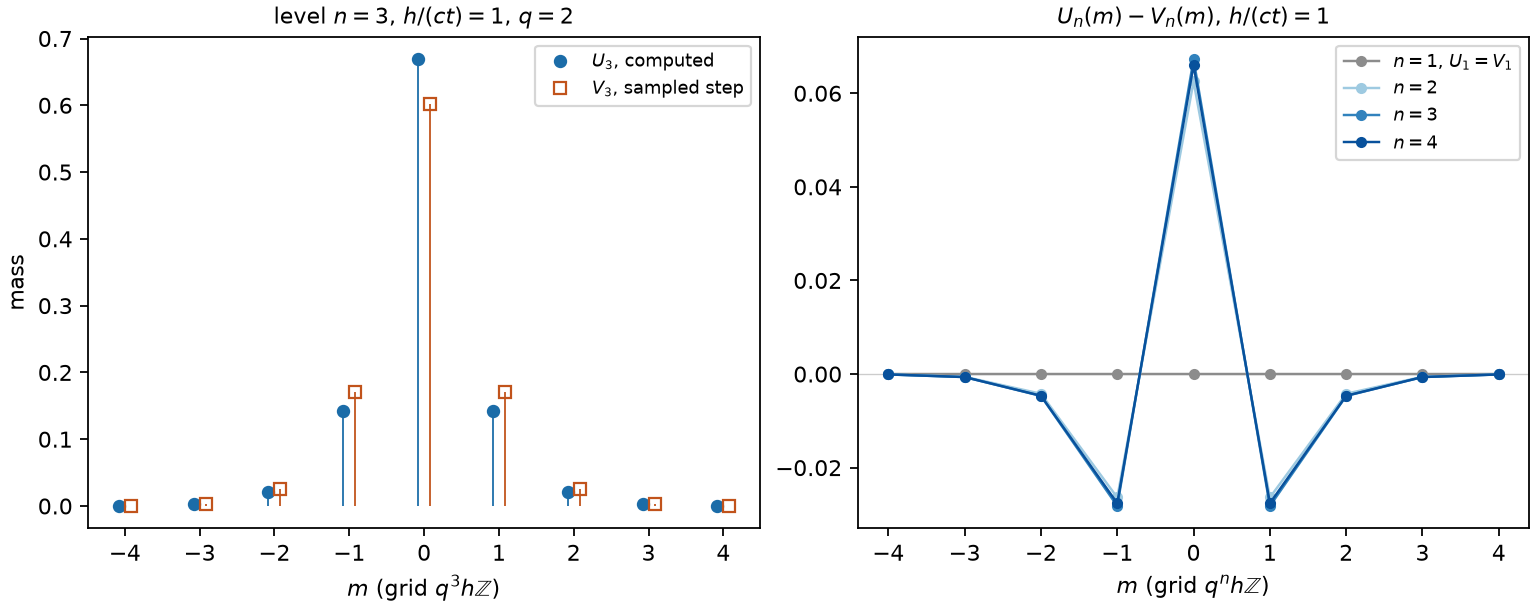
\includegraphics[width=\textwidth]{theory-grid-steps.png}
\caption{Proposition~\ref{prop:sampled-laplace-exact}(2) at $q = 2$ and $h/(ct) = 1$, in the units
of the grid $q^nh\ZZ$. Left: the computed array $U_3$, from $u_0 = \delta_0$ by three levels of
recursion and decimation, and the sampled step $V_3$, the samples of
$L_{ct} * L_{ctq} * L_{ctq^2}$ on $q^3h\ZZ$, both renormalized to unit mass. Right:
$U_n(m) - V_n(m)$ for $n = 1, \dots, 4$. At $n = 1$ the run gives at most $10^{-16}$, which is
rounding. From $n = 2$ on, the difference at the centre lies between $0.062$ and $0.068$. Half the
$\ell^1$ norm of the difference is the distance of Table~\ref{tab:grid-pyramid-error}.}
\label{fig:theory-grid-steps}
\end{figure}

The samples of the Gaussian kernel on a grid, the first family one would try there, do not form a
convolution semigroup [\sscite{lindeberg1990scalespace}, Prop.~12 and the remark after it, p.~242]. Renormalized, they need not
form a hemigroup either. The script \texttt{scripts/sampled\_gaussian\_increments.py} computes the
step between two renormalized sampled Gaussians, as the inverse transform of the ratio of their
discrete transfers, for four pairs of standard deviations in grid units. Each Gaussian is sampled
at the $4096$ sites $-2048, \dots, 2047$, renormalized there, and read on the periodic grid of those
sites. Between $0.5$ and $0.6$ the step's least coefficient is $-0.011$, and between $1.0$ and
$1.2$ it is $-0.0046$, both at the sites $\pm 2$. Between $2.0$ and $2.5$ the least coefficient is
$-2.8 \times 10^{-7}$, at $\pm 10$. Between $0.7$ and $3.0$ the double-precision value is rounding.
The script evaluates that pair again at $60$ digits, and the least coefficient is
$-2.8 \times 10^{-33}$, at $\pm 36$. These are computed signs on a periodic grid. Over the four
pairs the magnitude of the least coefficient falls as the larger standard deviation grows, and no inequality is proved here for
all scales.

For the first pair a short argument shows on the infinite lattice $\ZZ$ that no probability law
joins the two. Let $X$ and $Z$ have the sampled Gaussian laws of standard deviations $0.5$ and
$0.6$, normalized on $\ZZ$. Suppose $Z$ has the law of $X + Y$, with $Y$ a random variable
independent of $X$. Then $Y$ lives on $\ZZ$, since
$X$ has an atom at $0$. Its moments are finite, as those of $Z$ are, and $\mathbb{E}Y = 0$. The
second and fourth moments give
$\mathbb{E}Y^2 = \mathbb{E}Z^2 - \mathbb{E}X^2$ and
$\mathbb{E}Y^4 = \mathbb{E}Z^4 - \mathbb{E}X^4 - 6\,\mathbb{E}X^2\,\mathbb{E}Y^2$. The script
computes them, with the sums cut at $|k| \le 5$ and an omitted tail below $10^{-18}$:
$\mathbb{E}Y^2 = 0.1366$ and $\mathbb{E}Y^4 = 0.0160$. On the integers $Y^4 \ge Y^2$, so
$\mathbb{E}Y^4 \ge \mathbb{E}Y^2$, a contradiction. So no probability law joins the two sampled
Gaussians, and the sampled Gaussian family is not a hemigroup on $\ZZ$. The argument fails at the
other three pairs, where
$\mathbb{E}Y^4 \ge \mathbb{E}Y^2$.

What the Laplace samples have and the Gaussian samples lack is the factorization of
Proposition~\ref{prop:sampled-laplace-exact}(1). Every step of the sampled Laplace family is a
convolution of two one-sided geometric laws, each mixed with $\delta_0$ at the weight
$p \in [0,1)$. The factorization rests on the transfer (\ref{eq:sampled-laplace-transfer}), a
rational function of $e^{i\vartheta}$ with one pole inside and one outside the unit circle. That the
mixing weight is a probability, $p < 1$, needs $a_s < a_t$ as well. The samples of a Gaussian have
a theta function as their transfer instead.

The sampled Laplace mask is also infinitely divisible on the grid, so its grid pyramid is exact in
sense (iii), in the second stratum (Proposition~\ref{prop:grid-pyramids-infinitely-divisible}(4)).
So the grid offers two objects. One is an exact cascade, the sampled Laplace family. The other is a
pyramid covariant under $q$, the geometric pyramid of its mask. For an integer $q \ge 2$, the
\Matern{} pyramid computed on the grids computes the ladder increments of the geometric pyramid of
the mask $g = \lambda_{ct}$ of Proposition~\ref{prop:sampled-laplace-exact}(2)
(Proposition~\ref{prop:line-and-arrays}(2)). From its second level on, its arrays are not the
samples of the \Matern{} pyramid's steps (Proposition~\ref{prop:sampled-laplace-exact}(2)).

\paragraph{Relation to the continuum theory.} Two statements used in this section have continuum
counterparts in the cone module \progpaper{V-cone v0.1}. They are Lindeberg's generator, from the
supplement, and the criterion for masks.

\emph{The generator.} The Cin ray of step $\tau$ \prog{V-cone v0.1}{Lemma~3.1(1), p.~13}, the fully
covariant family with the exponent $\Cin(\tau\omega)$, has at the scale $t$ the generator
$t^{-1}\delta^2_{t\tau}$, one symmetric second difference (Theorem~\ref{thm:cited-A13}). Its step
grows with the scale. Lindeberg's generator (Proposition~\ref{prop:lindeberg-stratum-one}) is the
same second difference, held at the fixed step $h$.

\emph{The masks.} The continuum counterpart of
Proposition~\ref{prop:grid-pyramids-infinitely-divisible}(2)--(3) is Theorem~\ref{thm:cited-A20}.
For a symmetric infinitely divisible step with a rational transform, it gives the covariant interpolant by a
product formula and decides whether that interpolant is the exponent of a fully covariant family.
The \Matern{} pyramid of Theorem~\ref{thm:matern-pyramid} at $d = 1$ is its case
$R(\omega) = (1 + \omega^2)^{-1}$ read at the scale $ct$. Its octave step from $t$ to $qt$ is the
Laplace law of range $ct$. On the lattice the picture changes in the following ways.
\begin{enumerate}
\item Infinite divisibility must be checked. The binomial mask has a rational transfer in
$e^{i\vartheta}$ and is not infinitely divisible, and clause (1) of the proposition supplies the
check.
\item The profile, a density in the continuum, becomes the finite atomic measure $\varpi_w$, and the
interpolant's becomes $\sum_mT_{q^{-m}}\varpi_w$. This is the same series read on measures, so the
product formula survives. Its convergence, automatic for a rational $R$, becomes the logarithmic
moment of the mask, the condition that makes the series of dilates a \Levy{} measure.
\item The continuum's criterion for full covariance has no lattice counterpart, as the opening of
Section~\ref{subsec:grid-pyramids-line} noted. The folded \Levy{} measures of a fully covariant
family are absolutely continuous (Theorem~\ref{thm:lattice-line}(3)), so an atomic one belongs to
no such family. Clause (3) gives the lattice answer: no grid pyramid is exact in the third stratum.
\end{enumerate}
When its criterion holds, Theorem~\ref{thm:cited-A20} delivers a fully covariant interpolant. A
grid pyramid requires covariance under one ratio only. In place of the uniqueness of the interpolant it has the uniqueness of the
knot kernels. Between the knots a grid pyramid is undetermined, and no fully covariant member is
there to select. The supplement describes this freedom (Section~\ref{sec:line-surface}).

% Transcribed from blueprint/src/parts/04-matern.tex.
\section{The \Matern{} pyramid}
\label{ch:matern}

Section~\ref{ch:pyramid} showed that covariance under one ratio admits many families, and that
between its knots a family is in general not fixed by its ladder. A designer who wants one pyramid
needs a further reason to choose. Scale-space theory gives such reasons as principles about what
smoothing may do to an image. On the line the classical principle is that smoothing creates no new
local extrema. The records of the line's \Matern{} pyramid obey it from rung to rung, for a suitable
class of inputs (Proposition~\ref{prop:ladder-non-creation-line}). In the plane this principle
fails. This section carries the \Matern{} pyramid to $\RR^d$, and gives a principle that holds in
the plane and selects it.

The pyramid is simple to describe. Its octave step from level $t$ to level $qt$ applies the
resolvent $(I - c^2t^2\Delta)^{-1}$, for a constant $c > 0$. The operator $I - c^2t^2\Delta$ is the
modified Helmholtz, or screened Poisson, operator. This section calls it the Helmholtz operator for
short, and its inverse the Helmholtz resolvent. Applying the resolvent to an image $u$ gives the
solution $v$ of $v - u = c^2t^2\Delta v$. That is one implicit Euler step, with the step size
$c^2t^2$, of the heat equation $\partial_\tau v = \Delta v$. So the pyramid runs the heat equation by
implicit steps, one per octave, and the step size grows by the factor $q^2$ from each octave to the
next.

The principle that selects it is a maximum principle for one such step. Required of every octave
step, it selects the \Matern{} pyramid among the isotropic families covariant under $q$, with the
scales labelled so that dilating the kernel at $t$ by $q$ gives the kernel at $qt$, up to a
relabelling in
$\mathcal{G}_q$. The subsections build to that result.
\begin{itemize}
\item Section~\ref{sec:matern-levels} constructs the pyramid in $\RR^d$ and looks at its octave
step as a computation.
\item Section~\ref{sec:matern-counting} shows that the line's reason for preferring the pyramid,
that it creates no extrema, does not carry to $d \ge 2$.
\item Section~\ref{sec:matern-selection} gives a reason that does. \emph{Non-enhancement} of local
extrema requires that smoothing not raise a local maximum or lower a local minimum. Read at one
finite step, it holds among the symmetric rotation-invariant laws exactly for the Helmholtz
resolvents $(I - \tau\Delta)^{-1}$, $\tau \ge 0$, the identity among them
(Proposition~\ref{prop:stage-lemma}). Then take an isotropic family covariant under $q$, in the
canonical discrete gauge. Required of one octave step, the principle fixes only the ladder through
it. Required of every octave step $\mu_{t,qt}$, from every scale $t \in [1, q)$, it selects the
\Matern{} pyramid up to the gauge $\chi \in \mathcal{G}_q$
(Theorem~\ref{thm:selection-stratum-two}(1)--(2)).
\end{itemize}

The section compares the plane with the line throughout. The statements on the line that it cites
are proved in Section~\ref{ch:line-appendix} of the supplement.
\begin{itemize}
\item The \Matern{} pyramid on the line, with its octave identity, generator and limit
$q \downarrow 1$ (Theorem~\ref{thm:matern-pyramid-line}).
\item Its \Polya{} frequency kernels and steps (Theorem~\ref{thm:matern-pyramid-line-noncreation}).
\item The counts from rung to rung (Proposition~\ref{prop:ladder-non-creation-line}).
\item The sums of Laplace atoms, the exponents $\log(1 + \omega^2/\vartheta^2)$ of two-sided
exponential laws, which are admissible when $\sum_i\vartheta_i^{-2} < \infty$
(Lemma~\ref{lem:laplace-atoms-admissible}).
\item The selection by phase entropy (Theorem~\ref{thm:phase-entropy-selection}).
\end{itemize}

\subsection{The levels and the octave step}
\label{sec:matern-levels}

What are the levels of the \Matern{} pyramid in $\RR^d$, and what must a pyramid compute to
produce them? The answer starts from the octave step, builds the family from it, and then looks at
the octave step again as a computation.
\begin{itemize}
\item The octave step: the law $L_r$, its density, and the profile $b_d$ of its \Levy{} measure
(Definition~\ref{def:matern-pyramid-data}, Lemmas~\ref{lem:bessel-profile}
and~\ref{lem:bessel-k}).
\item The pyramid: its existence and uniqueness, its projections onto lines, its generator and its
limit as $q \downarrow 1$ (Theorem~\ref{thm:matern-pyramid}).
\item The steps between scales that are not a factor $q$ apart, and what becomes of the line's
Thorin property in the plane (Propositions~\ref{prop:matern-increments}
and~\ref{prop:thorin-in-dimension-d}).
\item The octave step as a computation. In $d \ge 2$ it does not split into first-order passes and
its density has no central value. In every dimension the difference of two levels is a Laplacian
(Lemma~\ref{lem:no-first-order-factorization}, Propositions~\ref{prop:matern-generator-octave}
and~\ref{prop:laplacian-pyramid}).
\item A separable twin, the frame \Matern{} pyramid, which the next two subsections compare with the
\Matern{} pyramid (Definition~\ref{def:frame-matern-pyramid}).
\end{itemize}

The octave step is the law $L_r$ with transform $(1 + r^2|\omega|^2)^{-1}$, at $r = ct$. The
literature knows it under several names, and they all denote this one law. Its density is
$r^{-d}G_2(x/r)$, with $G_2$ the Bessel potential of order $2$, the kernel of $(I - \Delta)^{-1}$
[\sscite{stein1970singular}, Ch.~V, \S 3, (26) and Prop.~2, p.~132], read in this paper's
convention for the transform. So $L_r$ is the Green's function of $I - r^2\Delta$. It is also the
\Matern{} law of index $1$ at range $r$. The laws with transform $(1 + r^2|\omega|^2)^{-\gamma}$ are
named after the \Matern{} covariances of spatial statistics
[\sscite{whittle1954stationary}, p.~448; \sscite{lindgren2011explicit}, (2), p.~426], and for $\gamma > d/2$ their
densities are those covariances (Section~\ref{ch:price}). In $d \ge 2$ the density of the octave
step, of index $1 \le d/2$, is not a \Matern{} covariance. No kernel $\mu_t$ of the \Matern{}
pyramid is a \Matern{} law, in any dimension. Read as a function of $|\omega|^2$, its transform is
singular at infinitely many points of the negative axis, and a \Matern{} transform at one. Finally, $L_r$ is the kernel of
\prog{iso v0.1}{Prop.~3.12(2), p.~16} at scale $\sqrt2\,r$. The paper writes $L_r$ for the law,
and the Helmholtz resolvent for the operator $f \mapsto L_r * f$. The name Bessel potential stays in
use for $L_r$ where the comparison with the literature needs it.

The definition below starts from one more description. The law $L_r$ is a Gaussian variance
mixture: the position at an exponential random time of a Brownian motion whose law at time $s$ is
$N(0, 2sI)$, the heat kernel of $\partial_\tau v = \Delta v$ at time $s$. This is the simplest case of
\emph{subordination}, which runs Brownian motion at a random time. The mixture gives the transform
and the density of $L_r$ at once. The definition also introduces the two functions that the rest of
the subsection uses. The exponent $F_q$ of the \Matern{} pyramid is the sum of the exponents of its
octave steps at the finer scales. The function $b_d$ describes the \Levy{} measure of $L_1$ in polar
coordinates. It is the polar profile of $L_1$, in the sense of Section~\ref{ch:cited}, and
$b_d(\cdot/r)$ is that of $L_r$ (Lemma~\ref{lem:bessel-profile}(2)).

% shared with blueprint def:matern-pyramid-data
\begin{definition}[the octave step and the \Matern{} exponent]
\label{def:matern-pyramid-data}

Fix $d \ge 1$. For $r > 0$ let
\[
  L_r := \int_0^\infty e^{-s}\,N(0, 2sr^2I)\,ds ,
\]
the law of $r\sqrt{2X}\,Z$ with $X$ standard exponential and $Z$ standard normal on $\RR^d$
independent of it. Call $L_r$ the \emph{\Matern{} law of index $1$ at range $r$}, and write $L_r$
also for the operator $f \mapsto L_r * f$. For $q > 1$ and $c > 0$ put
\[
  F_q(r) := \sum_{i \ge 1}\log\bigl(1 + c^2q^{-2i}r^2\bigr), \qquad
  b_d(y) := \frac{2}{\Gamma(d/2)}\int_0^\infty v^{d/2-1}e^{-v-y^2/(4v)}\,dv ,
  \qquad r, y \ge 0 .
\]
The series converges, each term being at most $c^2q^{-2i}r^2$.
\end{definition}

% shared with blueprint lem:bessel-profile
\begin{lemma}[the octave step and its profile]
\label{lem:bessel-profile}

Let $d \ge 1$ and $r > 0$.
\begin{enumerate}
\item $\widehat{L_r}(\omega) = (1 + r^2|\omega|^2)^{-1}$. The law $L_r$ has the density
$r^{-d}G(x/r)$, where
\[
  G(x) := \int_0^\infty e^{-s}(4\pi s)^{-d/2}e^{-|x|^2/(4s)}\,ds \in (0, \infty]
\]
is continuous on $\RR^d \setminus \{0\}$. For every $g \in L^1(\RR^d)$,
$(I - r^2\Delta)(L_r * g) = g$ in the sense of distributions.
\item For every $\beta > 0$ and $\omega \in \RR^d$,
\[
  \log\bigl(1 + \beta|\omega|^2\bigr)
   = \int_{\RR^d}\bigl(1 - \cos\langle\omega, x\rangle\bigr)\,
     \frac{b_d(|x|/\sqrt\beta)}{|S^{d-1}|\,|x|^d}\,dx .
\]
\item $b_d(0) = 2$, and $b_d$ is continuous and strictly decreasing on $[0, \infty)$, with
$b_d(y) \le C_de^{-y/2}$, $C_d := 2^{1+d/2}$. Further $b_1(y) = 2e^{-y}$ and
$b_3(y) = 2(1 + y)e^{-y}$.
\end{enumerate}
\end{lemma}

\begin{proof}
\emph{(1)} The law $L_r$ is the image of $L_1$ under $x \mapsto rx$, and $L_1$ is the law of
$\sqrt{2X}\,Z$. Given $X = s$, the vector $\sqrt{2s}\,Z$ has the law $N(0, 2sI)$, with the transform
$e^{-s|\omega|^2}$ and the density $g_{2s}(x) := (4\pi s)^{-d/2}e^{-|x|^2/(4s)}$. Integrating against
$e^{-s}\,ds$ gives, by Tonelli's theorem, the transform
$\int_0^\infty e^{-s(1 + |\omega|^2)}\,ds = (1 + |\omega|^2)^{-1}$ of $L_1$. The function
$G = \int_0^\infty e^{-s}g_{2s}\,ds$ is integrable, and by Fubini's theorem its transform is the same
integral, $(1 + |\omega|^2)^{-1}$. By the uniqueness of the transform, $L_1$ has the density $G$.
The image under $x \mapsto rx$ then has the density $r^{-d}G(x/r)$ and the transform
$(1 + r^2|\omega|^2)^{-1}$. For $|x| \ge \delta > 0$ the integrand defining $G$ is at most
$e^{-s}(4\pi s)^{-d/2}e^{-\delta^2/(4s)}$, which is integrable in $s$. So $G$ is finite off the
origin, and, differentiating under the integral sign in $|x|^2$, it is smooth there.

For the Green's function let $g \in L^1(\RR^d)$, let $\varphi$ be real, smooth and of compact
support, and put $\psi := \varphi - r^2\Delta\varphi$. First, for every $z$,
\[
  \int\psi(z + y)\,L_r(dy) = \varphi(z) .
\]
Read $\varphi$ as a complex Schwartz function, and write $\mathcal{F}$ for the transform of the
$2\pi$ convention, $\mathcal{F}\varphi(\xi) := \int e^{-2\pi i\langle\xi, x\rangle}\varphi(x)\,dx =
\widehat\varphi(-2\pi\xi)$. Fourier inversion gives
$\varphi(x) = \int e^{2\pi i\langle\xi, x\rangle}\mathcal{F}\varphi(\xi)\,d\xi$, and the transform of
$\Delta\varphi$ is $-4\pi^2|\xi|^2\mathcal{F}\varphi$, so
$\psi(x) = \int e^{2\pi i\langle\xi, x\rangle}(1 + 4\pi^2r^2|\xi|^2)\mathcal{F}\varphi(\xi)\,d\xi$, an
absolutely convergent integral. By Fubini's theorem,
\[
  \int\psi(z + y)\,L_r(dy)
   = \int e^{2\pi i\langle\xi, z\rangle}(1 + 4\pi^2r^2|\xi|^2)\mathcal{F}\varphi(\xi)\,
     \widehat{L_r}(2\pi\xi)\,d\xi
   = \int e^{2\pi i\langle\xi, z\rangle}\mathcal{F}\varphi(\xi)\,d\xi = \varphi(z) .
\]
Second, $\psi$ is bounded, so $(x, y) \mapsto g(x - y)\psi(x)$ is integrable for
the product of $dx$ and $L_r(dy)$. Fubini's theorem and the translation $x = z + y$ give
\[
  \int(L_r * g)\,\psi = \int\int g(x - y)\psi(x)\,dx\,L_r(dy)
   = \int\int g(z)\psi(z + y)\,dz\,L_r(dy) = \int g(z)\varphi(z)\,dz .
\]
This is $(I - r^2\Delta)(L_r * g) = g$ in the sense of distributions.

\emph{(2)} Frullani's integral gives, for $u \ge 0$,
\[
  \log(1 + \beta u) = \int_0^\infty\bigl(1 - e^{-su}\bigr)\,e^{-s/\beta}\,\frac{ds}{s} .
\]
Both sides vanish at $u = 0$. For $u > 0$ put $a := 1/\beta$ and $b := u + 1/\beta$. The integrand is
$(e^{-as} - e^{-bs})/s = \int_a^be^{-ts}\,dt$, and Tonelli's theorem gives
$\int_a^b\int_0^\infty e^{-ts}\,ds\,dt = \int_a^bdt/t = \log(b/a) = \log(1 + \beta u)$.
Put $u = |\omega|^2$. Let $g_{2s}(x) := (4\pi s)^{-d/2}e^{-|x|^2/(4s)}$ be the density of
$N(0, 2sI)$. It is symmetric with mass $1$, so
$1 - e^{-s|\omega|^2} = \int(1 - \cos\langle\omega, x\rangle)\,g_{2s}(x)\,dx$. All integrands are
nonnegative, and Tonelli's theorem gives
$\log(1 + \beta|\omega|^2) = \int(1 - \cos\langle\omega, x\rangle)\,f_\beta(|x|)\,dx$ with
\[
  f_\beta(\rho) := \int_0^\infty(4\pi s)^{-d/2}e^{-\rho^2/(4s)}e^{-s/\beta}\,\frac{ds}{s} ,
  \qquad \rho > 0 .
\]
The substitution $s = \rho^2/(4v)$ has $ds/s = -dv/v$ and $(4\pi s)^{-d/2} = \pi^{-d/2}\rho^{-d}v^{d/2}$,
so $f_\beta(\rho) = \pi^{-d/2}\rho^{-d}\int_0^\infty v^{d/2-1}e^{-v-\rho^2/(4\beta v)}\,dv$. With
$|S^{d-1}| = 2\pi^{d/2}/\Gamma(d/2)$ this reads $|S^{d-1}|\,\rho^df_\beta(\rho) = b_d(\rho/\sqrt\beta)$.

\emph{(3)} At $y = 0$ the integral is $\Gamma(d/2)$, so $b_d(0) = 2$. For each $v > 0$ the integrand
is continuous and strictly decreasing in $y \ge 0$ and at most $v^{d/2-1}e^{-v}$, so $b_d$ is
continuous by dominated convergence and strictly decreasing. For the bound, split the exponent in
halves. The inequality of the means gives $\tfrac12\bigl(v + y^2/(4v)\bigr) \ge y/2$, and dropping
a term gives $\tfrac12\bigl(v + y^2/(4v)\bigr) \ge v/2$. So the integrand is at most
$e^{-y/2}v^{d/2-1}e^{-v/2}$, and
$b_d(y) \le e^{-y/2}\,\frac{2}{\Gamma(d/2)}\int_0^\infty v^{d/2-1}e^{-v/2}\,dv = 2^{1+d/2}e^{-y/2}$.

For the closed forms let $y > 0$; at $y = 0$ both read $b_d(0) = 2$. Put $\eta := y/2$ and
$E(w) := e^{-w^2 - \eta^2/w^2}$ for $w > 0$. The substitution $v = w^2$ gives
\[
  \int_0^\infty v^{\nu-1}e^{-v-y^2/(4v)}\,dv = 2\int_0^\infty w^{2\nu-1}E(w)\,dw .
\]
Since $w^2 + \eta^2/w^2 = 2\eta + (w - \eta/w)^2$, $E(w) = e^{-2\eta}e^{-(w - \eta/w)^2}$. Put
\[
  J_1 := \int_0^\infty e^{-(w - \eta/w)^2}\,dw , \qquad
  J_2 := \int_0^\infty \eta w^{-2}e^{-(w - \eta/w)^2}\,dw .
\]
The substitution $w \mapsto \eta/w$ maps $(0, \infty)$ onto itself and leaves $(w - \eta/w)^2$
unchanged, so $J_1 = J_2$. The map $\sigma(w) := w - \eta/w$ is an increasing bijection of
$(0, \infty)$ onto $\RR$ with the derivative $1 + \eta w^{-2}$, so
$J_1 + J_2 = \int_{\RR}e^{-\sigma^2}\,d\sigma = \sqrt\pi$. Hence $J_1 = J_2 = \tfrac12\sqrt\pi$, and
\[
  \int_0^\infty E(w)\,dw = \tfrac12\sqrt\pi\,e^{-2\eta} , \qquad
  \int_0^\infty w^{-2}E(w)\,dw = \frac{\sqrt\pi}{2\eta}\,e^{-2\eta} .
\]
At $\nu = 1/2$, with $\Gamma(1/2) = \sqrt\pi$, this gives
$b_1(y) = \frac{2}{\sqrt\pi}\cdot2\int_0^\infty E = 2e^{-y}$. At $\nu = 3/2$ the integral
$\int_0^\infty w^2E(w)\,dw$ is needed. The function $F(w) := wE(w)$ has the derivative
$F'(w) = (1 - 2w^2 + 2\eta^2w^{-2})E(w)$, and $F(w) \to 0$ as $w \to 0$ from above and as
$w \to \infty$, since $0 \le E(w) \le e^{-w^2}$. So $\int_0^\infty F' = 0$, that is
\[
  2\int_0^\infty w^2E(w)\,dw = \int_0^\infty E(w)\,dw + 2\eta^2\int_0^\infty w^{-2}E(w)\,dw
   = \tfrac12\sqrt\pi\,e^{-2\eta}(1 + 2\eta) .
\]
With $\Gamma(3/2) = \sqrt\pi/2$ this gives
$b_3(y) = \frac{4}{\sqrt\pi}\cdot\tfrac12\sqrt\pi\,(1 + y)e^{-y} = 2(1 + y)e^{-y}$.
\end{proof}

In the plane the profile is a modified Bessel function [\sscite{dlmf2026}], $b_2(y) = 2yK_1(y)$. The
next lemma gives this form in every dimension. It also proves the facts on $K_0$ that two later
proofs use: the limit profile in the plane, and the value of the density at its centre
(Propositions~\ref{prop:thorin-in-dimension-d} and~\ref{prop:matern-generator-octave}).

% shared with blueprint lem:bessel-k
\begin{lemma}[the profile through Bessel functions]
\label{lem:bessel-k}

Let $K_\nu$ be the modified Bessel function of the second kind of order $\nu$, and let $y > 0$.
\begin{enumerate}
\item For every real $\nu$,
\[
  \int_0^\infty v^{\nu-1}e^{-v-y^2/(4v)}\,dv = 2(y/2)^\nu K_\nu(y) .
\]
So $b_d(y) = \frac{4}{\Gamma(d/2)}(y/2)^{d/2}K_{d/2}(y)$, and $b_2(y) = 2yK_1(y)$.
\item $K_0$ is differentiable on $(0, \infty)$ with $K_0' = -K_1$, and $K_0(y) \to 0$ as
$y \to \infty$.
\item $K_0(y) = \int_1^\infty e^{-ys}(s^2 - 1)^{-1/2}\,ds$, and $K_0(y) - \log(1/y)$ stays bounded
as $y \downarrow 0$.
\end{enumerate}
\end{lemma}

\begin{proof}
\emph{(1)} DLMF~10.32.10 (\ledger{A51}), at $z = y$ and at the order $-\nu$, gives
$K_{-\nu}(y) = \tfrac12(\tfrac12y)^{-\nu}\int_0^\infty t^{\nu-1}e^{-t - y^2/(4t)}\,dt$. By
DLMF~10.32.9, $K_\nu(y) = \int_0^\infty e^{-y\cosh u}\cosh(\nu u)\,du$, which is even in $\nu$, so
$K_{-\nu} = K_\nu$ and the identity follows. The integral converges for every real $\nu$. The
substitution $v = \tfrac y2e^w$, under which $v + y^2/(4v) = y\cosh w$ and $dv/v = dw$, turns it into
$2(\tfrac y2)^\nu\int_0^\infty\cosh(\nu w)e^{-y\cosh w}\,dw$, and
$\cosh(\nu w)e^{-y\cosh w} \le e^{2\nu^2/y}e^{-(y/8)w^2}$ for $w \ge 0$, since
$\cosh(\nu w) \le e^{|\nu|w}$ and $\cosh w \ge w^2/4$. At $\nu = d/2$ the identity is the closed form
of $b_d$. At $d = 2$, $\Gamma(1) = 1$ gives $b_2(y) = 2yK_1(y)$.

\emph{(2)} By DLMF~10.32.9, $K_0(z) = \int_0^\infty e^{-z\cosh u}\,du$. For $|z - y| < y/2$ the
$z$-derivative of the integrand, $-\cosh u\,e^{-z\cosh u}$, is at most
$\cosh u\,e^{-(y/2)\cosh u}$ in absolute value, and the integral of this bound is $K_1(y/2)$, which is
finite by the bound in (1). So $K_0$ is differentiable at $y$ with
$K_0'(y) = -\int_0^\infty\cosh u\,e^{-y\cosh u}\,du = -K_1(y)$. For $y \ge 1$,
$(y - 1)(\cosh u - 1) \ge 0$ gives $y\cosh u \ge (y - 1) + \cosh u$, so
$0 \le K_0(y) \le e^{1-y}K_0(1)$, which tends to $0$ as $y \to \infty$.

\emph{(3)} The substitution $s = \cosh u$, with $ds = \sinh u\,du$ and
$\sinh u = (s^2 - 1)^{1/2}$, maps $(0,\infty)$ onto $(1,\infty)$ and turns
$K_0(y) = \int_0^\infty e^{-y\cosh u}\,du$ into the integral of (3), which therefore converges. For the
origin let $0 < y < 1$ and $L := \log(1/y) > 0$, so that $ye^L = 1$. On $(0, L]$ the integrand lies
between $1 - y\cosh u \ge 1 - ye^u$ and $1$, since $\cosh u \le e^u$. On $(L, \infty)$ it is positive
and, since $y\cosh u \ge \tfrac12ye^u = \tfrac12e^{u-L} \ge \tfrac12(u - L)$, at most
$e^{-(u-L)/2}$, whose integral over $(L,\infty)$ is $2$. Hence
\[
  L - (1 - y) = \int_0^L\bigl(1 - ye^u\bigr)\,du \le K_0(y) \le L + 2 ,
\]
and $|K_0(y) - \log(1/y)| \le 2$ for $0 < y < 1$.

The one cited fact is DLMF~10.32.10 (\ledger{A51}), read in (1); DLMF~10.32.9 is the definition of
$K_\nu$.
\end{proof}

The pyramid is built from these pieces. Its exponent at scale $t$ is $F_q(t|\omega|)$, the sum of
the exponents of the octave steps below $t$. The series telescopes,
$F_q(qr) - F_q(r) = \log(1 + c^2r^2)$, so the step from $t$ to $qt$ is the one law $L_{ct}$. The
next theorem shows that this exponent defines an isotropic family, covariant under every dilation.
Among continuous $F$ with $F(0) = 0$, the octave identity determines the exponent. Clause (1)
places $F_q$ in the class $\mathcal{A}_d$ of Section~\ref{subsec:cited-d}, the admissible $F$ for
which $F(|\cdot|)$ is the exponent of a self-decomposable law on $\RR^d$. The proof checks this
through the polar form of $\mathcal{A}_d$ (Theorem~\ref{thm:cited-A35}). The other clauses record
what later results use. They are the projections onto lines, where the line's counts survive for
suitable inputs, the generator, and the limit $q \downarrow 1$.

% shared with blueprint thm:matern-pyramid
\begin{theorem}[the \Matern{} pyramid in $\RR^d$]
\label{thm:matern-pyramid}

Fix $q > 1$, $c > 0$ and $d \ge 1$.
\begin{enumerate}
\item \emph{(Admissibility.)} $F_q \in \mathcal{A}_d$, with Gaussian coefficient $0$ and the
nonincreasing polar profile $k_d(r) = \sum_{i \ge 1}b_d(rq^i/c)$. So the transforms
$\exp\bigl[-\bigl(F_q(t|\omega|) - F_q(s|\omega|)\bigr)\bigr]$, $0 \le s \le t$, define an isotropic
family with $S_\lambda t = \lambda t$ for every $\lambda > 0$, the \emph{\Matern{} pyramid}. Its
octave step is one Bessel potential, $\mu_{t,qt} = L_{ct}$ for $t > 0$. Its kernel is the Gaussian variance
mixture $\mu_t = \mathrm{law}\bigl(\sqrt{2V_t}\,Z\bigr)$, with
$V_t = \sum_{i \ge 1}c^2q^{-2i}t^2X_i$, the $X_i$ independent standard exponential and $Z$ standard
normal on $\RR^d$ independent of them, and for $t > 0$ it has a $C^\infty$ density with all
derivatives bounded.
\item \emph{(Uniqueness.)} If $\widetilde F$ is continuous on $[0, \infty)$ with $\widetilde F(0) = 0$
and $\widetilde F(qr) - \widetilde F(r) = \log(1 + c^2r^2)$ for $r \ge 0$, then $\widetilde F = F_q$.
An isotropic fully covariant family $(\mu'_{s,t})$ whose kernels $\mu'_{0,q^n}$, $n \in \ZZ$, have
the transforms $\exp\bigl(-F_q(q^n|\omega|)\bigr)$ is the family of (1) read in a gauge $\chi$ with
$\chi(q^n) = q^n$ for every $n$.
\item \emph{(Projections.)} Along every unit vector $e$, the marginal family
$\bigl(\langle e, \cdot\rangle_*\mu_{s,t}\bigr)$ is the \Matern{} pyramid on the line of
Theorem~\ref{thm:matern-pyramid-line}. For $f \in L^1(\RR^d)$ and $t > 0$ call $\mu_t * f$ the
\emph{record} of $f$ at scale $t$. Its projection along $e$, the density of the image of
$(\mu_t * f)(x)\,dx$ under $x \mapsto \langle e, x\rangle$, is the \emph{projected record}. It is
the projection of $f$ convolved with a \Polya{} frequency density. Suppose that the projection of
$f$ has a version that is the primitive of an integrable function. Then for every $t > 0$ the
projected record at scale $t$ crosses each level no more often, and changes monotonicity no more
often, than that version. Under the same hypothesis, for every $s > 0$ the projected record at
scale $qs$ crosses each level no more often, and changes monotonicity no more often, than the
projected record at scale $s$.
\item \emph{(Generator.)} For $f \in \mathcal{S}(\RR^d)$ and $t > 0$,
$\partial_t(\mu_t * f) = \mathcal{H}_t(\mu_t * f)$ almost everywhere, with
$\mathcal{H}_t = \frac2t\sum_{i \ge 1}(L_{ctq^{-i}} - I)$, a series of bounded operators on
$L^1(\RR^d)$ that converges absolutely in $L^1$ on $W^{2,1}(\RR^d)$ and whose sum is not bounded in
the $L^1$ norm.
\item \emph{(The limit $q \downarrow 1$.)} With $\ell = \log q$, $\ell F_q(r) \to \Lambda(r) :=
-\tfrac12\operatorname{Li}_2(-c^2r^2)$ locally uniformly as $q \downarrow 1$, and
$\Lambda \in \mathcal{A}_d$ for every $d$, with polar profile $\int_0^\infty b_d(re^u/c)\,du$. The
laws with exponent $\ell F_q(t|\cdot|)$ exist, and they converge weakly at every scale to the law
with exponent $\Lambda(t|\cdot|)$. The kernels $\mu_t$, $t > 0$, themselves do not converge:
$\widehat{\mu_t}(\omega) = e^{-F_q(t|\omega|)} \to 0$ for $\omega \ne 0$.
\end{enumerate}
\end{theorem}

\begin{proof}
\emph{(1)} By Lemma~\ref{lem:bessel-profile}(2) with $\beta = c^2q^{-2i}$,
\[
  \log\bigl(1 + c^2q^{-2i}|\omega|^2\bigr)
   = \int_{\RR^d}\bigl(1 - \cos\langle\omega, x\rangle\bigr)\,
     \frac{b_d(|x|q^i/c)}{|S^{d-1}|\,|x|^d}\,dx .
\]
Summing over $i$, by Tonelli's theorem,
\[
  F_q(|\omega|) = \int_{\RR^d}\bigl(1 - \cos\langle\omega, x\rangle\bigr)\,
   \frac{k_d(|x|)}{|S^{d-1}|\,|x|^d}\,dx , \qquad k_d(r) = \sum_{i \ge 1}b_d(rq^i/c) .
\]
This is the exponent of the datum $(0, k_d)$ in the normalization of
Definition~\ref{def:isotropic-origin-data}, whose \Levy{} measure has the radial density
$k_d(|x|)\bigl(|S^{d-1}|\,|x|^d\bigr)^{-1}$. The profile $k_d$ is nonincreasing as a sum of
nonincreasing functions (Lemma~\ref{lem:bessel-profile}(3)).
Its integrability conditions follow from one bound. Since $e^{-x} \le 1/x$ for $x > 0$, the bound
$b_d(y) \le C_de^{-y/2}$ gives $b_d(y) \le 2C_d/y$, so
\[
  k_d(r) \le \sum_{i \ge 1}\frac{2C_dc}{rq^i} = \frac{M}{r} , \qquad M := \frac{2C_dc}{q - 1} ,
  \qquad r > 0 .
\]
Hence $k_d(r)\,r \le M$ on $(0, 1)$ and $k_d(r)/r \le M/r^2$ on $(1, \infty)$, and
$\int_0^1k_d(r)\,r\,dr \le M$, $\int_1^\infty k_d(r)\,dr/r \le M$. So $F_q \in \mathcal{A}_d$ by \ledger{A35}. It is not identically $0$, since $b_d > 0$, and that is the hypothesis
$F \not\equiv 0$ under which Theorem~\ref{thm:cited-A34} realizes a family.
By Theorem~\ref{thm:cited-A34} with $\chi = \mathrm{id}$ there is an isotropic family with
$\widehat{\mu_{s,t}}(\omega) = \exp\bigl[-\bigl(F_q(t|\omega|) - F_q(s|\omega|)\bigr)\bigr]$. Its
covariance is read off the transforms: $\widehat{\mu_{s,t}}(\lambda\omega) =
\widehat{\mu_{\lambda s,\lambda t}}(\omega)$, so $D_\lambda\mu_{s,t} = \mu_{\lambda s,\lambda t}$ by
the uniqueness of the transform. The telescoping is
$F_q(qr) = \sum_{i \ge 1}\log(1 + c^2q^{-2(i-1)}r^2) = \log(1 + c^2r^2) + F_q(r)$. It gives
$\widehat{\mu_{t,qt}}(\omega) = (1 + c^2t^2|\omega|^2)^{-1}$, so $\mu_{t,qt} = L_{ct}$ by
Lemma~\ref{lem:bessel-profile}(1).

For the mixture let $t \ge 0$ and put $a_i := c^2q^{-2i}t^2$. The exponential law is carried by
$(0, \infty)$ and has mean $1$, so by monotone convergence $E\sum_ia_iX_i = \sum_ia_i < \infty$, and
the series $V_t = \sum_ia_iX_i$ of nonnegative terms converges almost surely; what it is on the
exceptional null set does not change the law of $\sqrt{2V_t}\,Z$. The variable $V_t$ is a
measurable function of the sequence $(X_i)$, which is independent of $Z$, so the pair $(V_t, Z)$ has
the product law $\nu \otimes N(0, I)$, with $\nu$ the law of $V_t$. For fixed $v \ge 0$ the variable
$\sqrt{2v}\,Z$ has the transform $e^{-v|\omega|^2}$, so by Fubini's theorem the law of
$\sqrt{2V_t}\,Z$ has the transform $E\bigl[e^{-V_t|\omega|^2}\bigr]$. Let $u \ge 0$. For the
partial sums $V_t^{(N)} := \sum_{i \le N}a_iX_i$, independence and the transform
$E[e^{-uX_i}] = (1 + u)^{-1}$ of the exponential law give
$E\bigl[e^{-uV_t^{(N)}}\bigr] = \prod_{i=1}^N(1 + a_iu)^{-1}$. As $N \to \infty$ the left side tends
to $E[e^{-uV_t}]$ by dominated convergence, the integrands lying in $[0, 1]$, and the right side
tends to $\prod_{i \ge 1}(1 + a_iu)^{-1} = e^{-F_q(t\sqrt u)}$, the product (\ref{eq:line-e7}) of
Theorem~\ref{thm:matern-pyramid-line}. At $u = |\omega|^2$ this is
$e^{-F_q(t|\omega|)} = \widehat{\mu_t}(\omega)$, as $F_q(0) = 0$. So $\mu_t$ is the law of
$\sqrt{2V_t}\,Z$, by the uniqueness of the transform.

\emph{The density.} Let $t > 0$. For every integer $N \ge 1$, keeping the first $N$
terms of the series,
\[
  e^{-F_q(t|\omega|)} \le \prod_{i=1}^N\bigl(1 + c^2q^{-2i}t^2|\omega|^2\bigr)^{-1}
   \le \bigl(1 + c^2q^{-2N}t^2|\omega|^2\bigr)^{-N} .
\]
So $|\omega|^m e^{-F_q(t|\omega|)}$ is integrable for every $m \ge 0$: with $b := \min(1,
c^2t^2q^{-2N})$ and $2N > m + d$, it is at most
$b^{-N}|\omega|^m(1 + |\omega|^2)^{-N} \le b^{-N}(1 + |\omega|^2)^{-(2N - m)/2}$. Put
\[
  p_t(x) := (2\pi)^{-d}\int e^{-i\langle\omega, x\rangle}e^{-F_q(t|\omega|)}\,d\omega .
\]
It is real, as the integrand is even in $\omega$ up to conjugation, and differentiation under the
integral sign gives every derivative, bounded by
$(2\pi)^{-d}\int|\omega|^{|\alpha|}e^{-F_q(t|\omega|)}\,d\omega$. For a Schwartz function $\Phi$,
Fubini's theorem, Fourier inversion on the Schwartz space, the evenness of
$e^{-F_q(t|\omega|)}$ and the self-adjointness of the transform give
$\int\Phi\,p_t\,dx = \int\Phi\,d\mu_t$. Three consequences follow. First, $p_t \ge 0$: if
$p_t(x_0) < 0$, then $p_t < 0$ on a ball around $x_0$, and a smooth bump $\Phi \ge 0$ supported in
that ball with $\Phi(x_0) = 1$ has $\int\Phi\,p_t\,dx < 0 \le \int\Phi\,d\mu_t$. Second,
$\int p_t\,dx \le 1$: smooth bumps $0 \le \Phi_n \le 1$ equal to $1$ on the ball of radius $n$
have $\int\Phi_np_t\,dx = \int\Phi_n\,d\mu_t \le 1$, and Fatou's lemma passes to the limit. Third,
$\mu_t = p_t\,dx$: both are finite measures, and testing on $\Phi_n(x)e^{i\langle\omega, x\rangle}$,
which are Schwartz functions, and letting $n \to \infty$ by dominated convergence shows that their
transforms agree at every $\omega$.

\emph{(2)} Applying the equation at $q^{-n}r$ and summing over $n = 1, \dots, N$ gives
$\widetilde F(r) = \widetilde F(q^{-N}r) + \sum_{n=1}^N\log(1 + c^2q^{-2n}r^2)$. The first term tends
to $\widetilde F(0) = 0$ by continuity, and the sum tends to $F_q(r)$. For the family, let
$(\mu'_{s,t})$ be an isotropic fully covariant family (Definition~\ref{def:isotropic-cascade-family}) with the
stated kernels $\mu'_{0,q^n}$. By \ledger{A31} there are a gauge $\chi$, an
increasing homeomorphism of $[0, \infty)$, and an $F \in \mathcal{A}_d$ with
$\widehat{\mu'_{s,t}}(\omega) = \exp\bigl(-[F(\chi(t)|\omega|) - F(\chi(s)|\omega|)]\bigr)$, the pair
unique up to $(\chi, F) \mapsto (a\chi, F(a^{-1}\,\cdot))$, $a > 0$. Choose $a$ so that
$\chi(1) = 1$. Since $\chi(0) = 0$ and $F(0) = 0$, the kernel $\mu'_{0,1}$ has the transform
$e^{-F(|\omega|)} = e^{-F_q(|\omega|)}$, so $F = F_q$. At the scale $q^n$,
$F_q(\chi(q^n)r) = F_q(q^nr)$ for every $r$. As $F_q$ is strictly increasing, $\chi(q^n) = q^n$. So
$\mu'_{s,t} = \mu_{\chi(s),\chi(t)}$.

\emph{(3)} Write $\pi := \langle e, \cdot\rangle$. The transform of an image measure is
$\widehat{\pi_*\mu}(r) = \widehat\mu(re)$, so $\pi_*\mu_{s,t}$ has the transform
$r \mapsto \widehat{\mu_{s,t}}(re) = \exp\bigl[-\bigl(F_q(t|r|) - F_q(s|r|)\bigr)\bigr]$. (For an
isotropic family this is Lemma~\ref{lem:reduction-keeps-stratum}'s identity
$\widehat{\mu_{s,t}}(\omega) = \widehat{m_{s,t}}(|\omega|)$ for the marginal laws
$m_{s,t} := \pi_*\mu_{s,t}$; the proof needs only the transform of the image.) These are the
transforms of the family of Theorem~\ref{thm:matern-pyramid-line}, with the same $q$ and $c$, and
the uniqueness of the transform identifies the laws. For $f \in L^1(\RR^d)$ write $P_ef$ for the
density of $\pi_*(f(x)\,dx)$, in $L^1(\RR)$ by Fubini's theorem. For a probability measure $\mu$
and bounded measurable $\phi$ on $\RR$, Fubini's theorem gives
\[
  \begin{aligned}
  \int\phi(\langle e, x\rangle)\,(\mu * f)(x)\,dx
   &= \iint\phi\bigl(\langle e, y\rangle + \langle e, z\rangle\bigr)f(y)\,dy\,\mu(dz) \\
   &= \iint\phi(\sigma + w)\,P_ef(\sigma)\,d\sigma\,(\pi_*\mu)(dw) ,
  \end{aligned}
\]
so $P_e(\mu * f) = (\pi_*\mu) * P_ef$. With $\mu = \mu_t$ this is the projection of $f$ convolved with
$\pi_*\mu_t$, a \Polya{} frequency density by Theorem~\ref{thm:matern-pyramid-line-noncreation}.
So the projected record at scale $t$ is $(\pi_*\mu_t) * P_ef$, the record at scale $t$ of the
signal $P_ef$ in the line's \Matern{} pyramid. For the counts let $g$ be a version of $P_ef$ that
is the primitive of an integrable $g'$. A convolution does not see the choice of version, so
$(\pi_*\mu_t) * P_ef = (\pi_*\mu_t) * g$ for every $t > 0$. The count from rung to rung is
Proposition~\ref{prop:ladder-non-creation-line}(2) for the signal $g$ at the scale $s$, whose
hypotheses hold: the line's \Matern{} pyramid has the exponent of that proposition with $a = 0$ and
$\vartheta_i = q^i/c$, so $\sum_i\vartheta_i^{-2} < \infty$ and $\mathrm{mult}(q\vartheta) -
\mathrm{mult}(\vartheta)$ is $1$ at $\vartheta = 1/c$ and $0$ elsewhere, and $g$ is the primitive of
an integrable function. The count from scale zero is the counting clause
\ledger{A23} for the same exponent and the same
signal, whose hypotheses hold as $\sum_i(q^i/c)^{-2} < \infty$ and $g$ is the primitive of an
integrable $g'$; it gives $S^-(u(t, \cdot) - y) \le S^-(g - y)$ for every level $y$ and
$S^-(\partial_xu(t, \cdot)) \le S^-(g')$ for the record $u(t, \cdot) = (\pi_*\mu_t) * g$ at every
$t > 0$, $S^-$ counting sign changes.

\emph{(4)} For $r > 0$ the law $L_r$ is a probability measure, so $\|L_r * g\|_1 \le \|g\|_1$ and
$L_r - I$ is bounded on $L^1$, with norm at most $2$. Let $g \in W^{2,1}(\RR^d)$, with the weak
second derivatives $v_j := \partial_j^2g \in L^1$. Weak derivatives pass through a finite measure:
for a test function $\varphi$, Fubini's theorem and the translation $x = z + y$ give
\[
  \int(L_r * g)\,\partial_j^2\varphi
   = \iint g(z)\,\partial_j^2\varphi(z + y)\,dz\,L_r(dy)
   = \iint v_j(z)\,\varphi(z + y)\,dz\,L_r(dy) = \int(L_r * v_j)\,\varphi ,
\]
a translate of a test function being a test function. The same computation with
$\partial^\alpha\varphi$ in place of $\partial_j^2\varphi$, for every multi-index $|\alpha| \le 2$,
gives $\int(L_r * g)\,\partial^\alpha\varphi = (-1)^{|\alpha|}\int(L_r * \partial^\alpha g)\,\varphi$,
with $\partial^\alpha g \in L^1$ the weak derivative of $g$. So $L_r * g$ has the weak derivatives
$L_r * \partial^\alpha g$, of $L^1$ norm at most $\|\partial^\alpha g\|_1$, and lies in
$W^{2,1}$; the argument reads of $L_r$ only that it is a probability measure. With the Green identity
$\int(L_r * g)(\varphi - r^2\Delta\varphi) = \int g\varphi$ of Lemma~\ref{lem:bessel-profile}(1),
for real $\varphi$, this gives
\[
  \int\Bigl(L_r * g - g - r^2\sum_jL_r * v_j\Bigr)\varphi = 0
\]
for every real smooth compactly supported $\varphi$. So $L_r * g - g = r^2L_r * \Delta g$ almost
everywhere, with $\Delta g := \sum_jv_j$, and $\|(L_r - I)g\|_1 \le r^2\sum_j\|v_j\|_1$. With
$r_i := ctq^{-i}$, $\sum_ir_i^2 = c^2t^2/(q^2 - 1)$, the series $\mathcal{H}_tg$ converges
absolutely in $L^1$.

The sum is not bounded. The transform of an integrable $g$ is that of the measure $g(x)\,dx$,
$\widehat g(\omega) := \int e^{i\langle\omega, x\rangle}g(x)\,dx$, so that
$|\widehat g(\omega)| \le \|g\|_1$. For $g \in W^{2,1}$ the absolute convergence lets the series
be integrated term by term, and Fubini's theorem gives $\widehat{L_r * g} = \widehat{L_r}\,\widehat g$,
so
\[
  \widehat{\mathcal{H}_tg}(\omega)
   = \frac2t\sum_{i \ge 1}\Bigl(\frac{1}{1 + r_i^2|\omega|^2} - 1\Bigr)\widehat g(\omega) .
\]
Suppose that $\|\mathcal{H}_tg\|_1 \le B\|g\|_1$ for every $g \in W^{2,1}$, and let $N \ge 1$ be an
integer. Take $\omega$ with $|\omega| = q^N/(ct)$, which exists as $d \ge 1$. Every term of the sum
is at most $0$, and for $i \le N$, $r_i|\omega| = q^{N-i} \ge 1$, so the term is at most
$-\tfrac12$. Let $g \ge 0$ be a smooth function with $\int g = 1$ supported in the ball of radius
$\varepsilon := 1/(2|\omega|)$ about the origin; it is a Schwartz function, so it is in $W^{2,1}$,
and $\|g\|_1 = 1$. Since $|e^{i\theta} - 1| \le |\theta|$,
$|\widehat g(\omega) - 1| \le \int g(x)\,|\langle\omega, x\rangle|\,dx \le \varepsilon|\omega| = \tfrac12$,
so $|\widehat g(\omega)| \ge \tfrac12$. Hence
$B \ge \|\mathcal{H}_tg\|_1 \ge |\widehat{\mathcal{H}_tg}(\omega)| \ge \frac2t\cdot\frac N2\cdot\frac12
= \frac{N}{2t}$ for every $N$, a contradiction.

For the generator let $f \in \mathcal{S}(\RR^d)$ and $v(\tau, \cdot) := \mu_\tau * f$. A Schwartz
function is in $W^{2,1}$, its derivatives being its weak derivatives by integration by parts, so
$v(t, \cdot) \in W^{2,1}$ by the passage of weak derivatives through $\mu_t$ above. Write
$\mathcal{F}$ for the transform of the $2\pi$ convention, $\mathcal{F}f(\xi) := \int e^{-2\pi
i\langle\xi, x\rangle}f(x)\,dx = \widehat f(-2\pi\xi)$, and $s := 2\pi|\xi|$. Since
$\int e^{-2\pi i\langle\xi, y\rangle}\mu_\tau(dy) = \widehat{\mu_\tau}(-2\pi\xi) = e^{-F_q(\tau s)}$,
Fourier inversion on the Schwartz space and Fubini's theorem give, for $\tau \ge 0$ and every $x$,
\[
  v(\tau, x) = \int e^{2\pi i\langle\xi, x\rangle}e^{-F_q(\tau s)}\,
    \mathcal{F}f(\xi)\,d\xi .
\]
By Theorem~\ref{thm:matern-pyramid-line}(3), $\partial_\tau e^{-F_q(\tau s)} = h_\tau(s)e^{-F_q(\tau s)}$
with $h_\tau(s) = \frac2\tau\sum_{i \ge 1}\bigl((1 + c^2\tau^2q^{-2i}s^2)^{-1} - 1\bigr)$, and
$|h_\tau(s)| \le 2\tau s^2\sum_ic^2q^{-2i}$, since $|(1 + a)^{-1} - 1| \le a$ for $a \ge 0$. So for
$\tau \in (t/2, 2t)$ the derivative of the integrand in $\tau$ is at most $A|\xi|^2|\mathcal{F}f(\xi)|$
in modulus, with $A$ a constant, an integrable bound, and differentiation under the integral sign
gives, at every $x$,
\[
  \partial_tv(t, x) = \int e^{2\pi i\langle\xi, x\rangle}h_t(s)e^{-F_q(ts)}\,
    \mathcal{F}f(\xi)\,d\xi .
\]
On the other side, the same computation with $L_{r_i}$ in place of $\mu_\tau$, applied to the
function $v(t, \cdot)$ written as above, gives
\[
  (L_{r_i} * v(t, \cdot))(x) - v(t, x)
   = \int e^{2\pi i\langle\xi, x\rangle}\Bigl(\frac{1}{1 + r_i^2s^2} - 1\Bigr)
     e^{-F_q(ts)}\,\mathcal{F}f(\xi)\,d\xi .
\]
These integrands are at most $r_i^2s^2|\mathcal{F}f(\xi)|$ in modulus, a bound summable in $i$ and
integrable in $\xi$, so the sum over $i$ may be taken under the integral sign, and $\frac2t$ times the
sum of the factors $(1 + r_i^2s^2)^{-1} - 1$ is $h_t(s)$. So
$\mathcal{H}_tv(t, \cdot)(x) = \partial_tv(t, x)$ at every $x$, and in particular almost everywhere.

\emph{(5)} For fixed $r$, $g_r(u) := \log(1 + c^2r^2e^{-2u})$ is decreasing and integrable on
$[0, \infty)$, and $\ell F_q(r) = \ell\sum_{i \ge 1}g_r(i\ell)$ is a Riemann sum of it. As in
Theorem~\ref{thm:matern-pyramid-line}(4), a statement in $r$ alone, $\ell F_q(r) \to \int_0^\infty
g_r(u)\,du = -\tfrac12\operatorname{Li}_2(-c^2r^2) = \Lambda(r)$, locally uniformly in $r$. For the
profile, Lemma~\ref{lem:bessel-profile}(2) with $\beta = c^2e^{-2u}$ and Tonelli's theorem in $u$
give $\Lambda(|\omega|) = \int(1 - \cos\langle\omega, x\rangle)\,k(|x|)\,
\bigl(|S^{d-1}|\,|x|^d\bigr)^{-1}dx$ with $k(r) := \int_0^\infty b_d(re^u/c)\,du$, nonincreasing.
Its integrability conditions hold: $b_d(y) \le 2C_d/y$ gives
$k(r) \le \int_0^\infty 2C_dc\,e^{-u}\,du/r = 2C_dc/r$, and the argument of (1) applies. So
$\Lambda \in \mathcal{A}_d$ by
\ledger{A35}. A positive multiple of an origin datum
is an origin datum, with the multiple of its exponent, so $\ell F_q \in \mathcal{A}_d$, by the same
proposition, and the law with exponent $\ell F_q(t|\cdot|)$ exists by the definition of
$\mathcal{A}_d$. Its transform converges at every $\omega$ to $e^{-\Lambda(t|\omega|)}$, the transform
of a law, so the laws converge weakly by Lévy's continuity theorem. For $r > 0$,
$F_q(r) = \ell F_q(r)/\ell \to \infty$, since $\Lambda(r) > 0$ and $\ell \to 0$. So
$\widehat{\mu_t}$ tends to the indicator of $\{0\}$.
The kernels have no weak limit: a weak limit $\nu$ in $\RR^d$ would give, testing on
$\phi(\langle e, \cdot\rangle)$ for a unit vector $e$ and $\phi$ bounded and continuous on $\RR$,
the weak limit $\langle e, \cdot\rangle_*\nu$ of the kernels $\langle e, \cdot\rangle_*\mu_t$ of
the line's \Matern{} pyramids (clause (3)), which have none
(Theorem~\ref{thm:matern-pyramid-line}(4)).
\end{proof}

At $d = 1$ this is Theorem~\ref{thm:matern-pyramid-line}. Comparing the two shows what the plane
keeps of the line and what it changes.

The octave step is kept. The telescoping $F_q(qr) - F_q(r) = \log(1 + c^2r^2)$ is a statement in
$r$ alone, so in every dimension one octave is the single law $L_{ct}$. Full covariance is kept too.
It needs only a nonincreasing polar profile with the two integrability conditions, and $k_d$ has
them.

The finer structure of the profile changes. On the line the profile is also completely monotone,
and that makes the \Matern{} pyramid a Thorin family there
(Theorem~\ref{thm:matern-pyramid-line}(1)). Its exponents lie in the symmetric Thorin class, a
Gaussian term plus a mixture of Laplace atoms $\log(1 + \omega^2/\vartheta^2)$. For $d \ge 2$
neither one term $b_d$ nor the sum $k_d$ is completely monotone, for any $q$
(Proposition~\ref{prop:thorin-in-dimension-d}).

The counts change as well. The counts of Proposition~\ref{prop:ladder-non-creation-line} survive on
the projections of clause (3), for an input whose projection has a version that is the primitive of
an integrable function. These projections are the marginals of
Lemma~\ref{lem:reduction-keeps-stratum}, the Radon projections of tomography. On the image itself
the count of local maxima fails: at every rung, some input gains a local maximum
(Proposition~\ref{prop:creation-plane}).

Last, the selection. Theorem~\ref{thm:selection-stratum-two} holds in every dimension, the line
included. Required at every octave stage, the principle fixes the family up to the gauge. On the
line a second functional,
the phase entropy, chooses within one ladder. It measures how far the octave phases of the \Levy{}
data are from uniform, and on a ladder with a similarity member and no Gaussian part it picks that
member (Theorem~\ref{thm:phase-entropy-selection}). It rests on the theory of the line and is not
carried to $\RR^d$ here.

The pyramid also has a twin in time, through the \emph{subordination bridge} of
\prog{V-cone v0.1}{\S 4.2, p.~26}. The bridge substitutes $\sigma = r^2/2$. It reads a function of the
frequency $r$ as a function of the Laplace variable $\sigma$ of a subordinator, an increasing
\Levy{} process used as a random clock. Then $F_q(r) = \sum_{i \ge 1}\log(1 + 2c^2q^{-2i}\sigma)$.
This is the exponent, in the Laplace variable $\sigma$, of Lindeberg's time-causal limit kernel
with ratio $q^2$ and constant $2c^2$, a cascade of first-order integrators in time. Lindeberg
defines that kernel by an infinite product of first-order factors
[\sscite{lindeberg2016time}, Sect.~5, (38), p.~62] and realizes it by recursive first-order filters
[\sscite{lindeberg2016time}, Sect.~6.2, p.~64]. The ratio and the constant are this paper's reading
of his product. In the variables of Theorem~\ref{thm:matern-pyramid}(1), $\mu_t$ is the law of
$\sqrt{2V_t}\,Z$, and $2V_t$ has the law of that limit kernel with the time constants
$2c^2t^2q^{-2i}$: the kernel is a mixture of Gaussians over it. Read in the frequency variable $r$
instead, the product $e^{-F_q(r)}$ is the squared modulus of the transform of another member of his
family, the one of ratio $q$ with the time constants $cq^{-i}$, $i \ge 1$. Each factor
$(1 + c^2q^{-2i}r^2)^{-1}$ equals $|1 + icq^{-i}r|^{-2}$, a first-order causal factor composed with
its reflection. So on the line $\mu_t$ is the limit kernel of ratio $q$, with the time constants
$ctq^{-i}$, convolved with its reflection. That is the
identity behind the forward and backward recursions of the \Matern{} family on the line
(Theorem~\ref{thm:cited-A19}).

Propositions~\ref{prop:matern-increments} and~\ref{prop:thorin-in-dimension-d} below decide which
exponents and which profiles are completely monotone. A function is completely monotone when its
derivatives alternate in sign (Section~\ref{subsec:cited-bernstein}). By Bernstein's theorem it is
then a mixture of decaying exponentials (Theorem~\ref{thm:cited-A55}). It is the property of the
line's profile named above. To show that a function lacks it, the
proofs need a property that every completely monotone function has and that function fails. The
next three lemmas supply them.
\begin{itemize}
\item A completely monotone function is log-convex along every arithmetic progression
(Lemma~\ref{lem:cm-log-convex}).
\item If $f > 0$ is completely monotone and $e^{\lambda r}f(r)$ grows at most polynomially, then
$e^{\lambda r}f(r)$ does not grow at all (Lemma~\ref{lem:cm-exponential-rate}).
\item A geometric series of differences of exponentials, with no atom of one cancelling an atom of
the other, is not completely monotone (Lemma~\ref{lem:cm-uncancelled-atom}).
\end{itemize}

% shared with blueprint lem:cm-log-convex
\begin{lemma}[complete monotonicity along an arithmetic progression]
\label{lem:cm-log-convex}

Let $f$ be completely monotone on $(0, \infty)$ and $h \ge 0$.
\begin{enumerate}
\item $f - f(\cdot + h)$ is completely monotone on $(0, \infty)$.
\item $f(x + h)^2 \le f(x)f(x + 2h)$ for every $x > 0$.
\end{enumerate}
\end{lemma}

\begin{proof}
\emph{(1)} The $n$-th derivative of $f - f(\cdot + h)$ is $f^{(n)} - f^{(n)}(\cdot + h)$. The function
$(-1)^nf^{(n)}$ is nonincreasing on $(0, \infty)$, its derivative being
$(-1)^nf^{(n+1)} = -(-1)^{n+1}f^{(n+1)} \le 0$. So $(-1)^n\bigl(f^{(n)}(x) - f^{(n)}(x + h)\bigr) \ge 0$.

\emph{(2)} Fix $x > 0$. For a function $g$ let $L_g$ be the linear functional on $\RR[X]$ with
$L_g(X^k) = g(x + kh)$. Then $L_{g - g(\cdot + h)}(p) = L_g(p) - L_g(Xp)$, so
$L_g\bigl(X^k(1 - X)^{m+1}\bigr) = L_{g - g(\cdot + h)}\bigl(X^k(1 - X)^m\bigr)$. By (1) and induction on
$m$, simultaneously for every completely monotone $g$, $L_f\bigl(X^k(1 - X)^m\bigr) \ge 0$ for all
$k, m \ge 0$; the case $m = 0$ is $f(x + kh) \ge 0$. So the weights $w_k := L_f(b_{N,k})$ of the
Bernstein polynomials $b_{N,k} := \binom NkX^k(1 - X)^{N-k}$ are nonnegative. Applying $L_f$ to
$\sum_kb_{N,k} = 1$, $\sum_kk\,b_{N,k} = NX$ and $\sum_kk(k - 1)\,b_{N,k} = N(N - 1)X^2$ gives
$\sum_kw_k = f(x)$, $\sum_kk\,w_k = Nf(x + h)$ and $\sum_kk^2w_k = N(N - 1)f(x + 2h) + Nf(x + h)$. By
Cauchy--Schwarz, $\bigl(\sum_kk\,w_k\bigr)^2 \le \sum_kw_k\sum_kk^2w_k$, which after division by $N$
reads
\[
  N\bigl(f(x + h)^2 - f(x)f(x + 2h)\bigr) \le f(x)\bigl(f(x + h) - f(x + 2h)\bigr)
\]
for every $N \ge 1$. So $f(x + h)^2 - f(x)f(x + 2h) \le 0$.
\end{proof}

% shared with blueprint lem:cm-exponential-rate
\begin{lemma}[the exponential rate of a completely monotone function]
\label{lem:cm-exponential-rate}

Let $f > 0$ be completely monotone on $(0, \infty)$, and let $\lambda, C, R$ be real and $p \ge 0$ an
integer with $e^{\lambda r}f(r) \le C(1 + r)^p$ for $r \ge R$. Then $e^{\lambda r}f(r)$ is
nonincreasing on $(0, \infty)$. In particular, a function $f > 0$ on $(0, \infty)$ with such a bound
and with $e^{\lambda r}f(r)$ unbounded on $[1, \infty)$ is not completely monotone.
\end{lemma}

\begin{proof}
Let $0 < x < y$, $h := y - x$ and $a_n := e^{\lambda(x + nh)}f(x + nh) > 0$.
Lemma~\ref{lem:cm-log-convex}(2) at $x + nh$, multiplied by
$e^{2\lambda(x + (n+1)h)} = e^{\lambda(x + nh)}e^{\lambda(x + (n+2)h)}$, gives
$a_{n+1}^2 \le a_na_{n+2}$. So the ratios $a_{n+1}/a_n$ are nondecreasing, and
$a_n \ge a_0\rho^n$ with $\rho := a_1/a_0$. Suppose $\rho > 1$. For $n \ge \max(1, R/h)$,
$a_0\rho^n \le a_n \le |C|(1 + x + nh)^p \le |C|(1 + x + h)^pn^p$, against $n^p\rho^{-n} \to 0$. So
$a_1 \le a_0$, that is $e^{\lambda y}f(y) \le e^{\lambda x}f(x)$. For the last sentence: if $f$ were
completely monotone, $e^{\lambda r}f(r) \le e^\lambda f(1)$ for every $r \ge 1$.
\end{proof}

% shared with blueprint lem:cm-uncancelled-atom
\begin{lemma}[an uncancelled atom]
\label{lem:cm-uncancelled-atom}

Let $0 < A < B$ and $\rho > 1$ with $A\rho^i \ne B\rho$ for every $i \ge 1$. Then
$g(x) := \sum_{i \ge 1}\bigl(e^{-A\rho^ix} - e^{-B\rho^ix}\bigr)$ is not completely monotone on
$(0, \infty)$.
\end{lemma}

\begin{proof}
Put $a_i := A\rho^i$ and $b_i := B\rho^i$. For $\vartheta, x > 0$,
$\vartheta^ne^{-\vartheta x} \le (n + 2)!\,x^{-n-2}\vartheta^{-2}$, and $\sum_ia_i^{-2}$,
$\sum_ib_i^{-2}$ are geometric. So the series of $g$ and of its termwise derivatives converge
uniformly on $(x_0, \infty)$ for every $x_0 > 0$, and
\[
  (-1)^ng^{(n)}(x) = \sum_ia_i^ne^{-a_ix} - \sum_ib_i^ne^{-b_ix} .
\]
Let $x_* := b_1$ and $h(u) := ue^{1-u}$. At $x = n/x_*$, $n \ge 1$,
\[
  \Bigl(\frac{e}{x_*}\Bigr)^n(-1)^ng^{(n)}\Bigl(\frac{n}{x_*}\Bigr)
   = \sum_ih\Bigl(\frac{a_i}{x_*}\Bigr)^n - \sum_ih\Bigl(\frac{b_i}{x_*}\Bigr)^n .
\]
Since $e^{u-1} \ge u$, with equality only at $u = 1$, $0 \le h(u) \le 1$ for $u \ge 0$ and
$h(u) < 1$ for $u \ne 1$. By hypothesis $a_i \ne x_*$ for every $i$; $b_1/x_* = 1$ and
$b_i/x_* = \rho^{i-1} > 1$ for $i \ge 2$. So the terms of the first sum tend to $0$ as $n \to \infty$,
and those of the second to $1$ for $i = 1$ and to $0$ otherwise. For $n \ge 1$, $h(u)^n \le h(u)$,
and $\sum_ih(a_i/x_*)$, $\sum_ih(b_i/x_*)$ converge, $h(\vartheta) = e\,\vartheta e^{-\vartheta} \le
6e\,\vartheta^{-2}$. By dominated convergence the right side tends to $0 - 1 = -1$, so
$(-1)^ng^{(n)}(n/x_*) < 0$ for large $n$, and $g$ is not completely monotone.
\end{proof}

A pyramid applies only the octave steps, but the family has a step between any two scales.
Smoothing from one level to a scale inside the next octave applies one of these other steps. The
octave step is a single Helmholtz resolvent. The steps between other pairs of scales are not, by
clause (3) of the next proposition, which says what they are.

It says so in the terms of the Bernstein functions of Section~\ref{subsec:cited-bernstein}. A
Bernstein function is a nonnegative function on $(0, \infty)$ whose derivative is completely
monotone. For a Bernstein function $f$ with $f(0{+}) = 0$, the function $e^{-f(|\omega|^2)}$ is the
transform of an infinitely divisible law in every dimension (\ledger{A57}). This is subordination
again, now with the standard Brownian motion, whose transform at time $1$ is $e^{-|\omega|^2/2}$.
It runs the heat equation $\partial_\tau v = \Delta v$ at half speed, and the factor $2$ below
compensates. Run at the random time of the subordinator with exponent $u \mapsto f(2u)$, it has
this law at time $1$.

% shared with blueprint prop:matern-increments
\begin{proposition}[the increments]
\label{prop:matern-increments}

Let $\beta > \gamma > 0$ and $f_{\beta,\gamma}(u) := \log\frac{1 + \beta u}{1 + \gamma u}$, $u \ge 0$.
\begin{enumerate}
\item $f_{\beta,\gamma}(u) = \int_{1/\beta}^{1/\gamma}\frac{u}{u + x}\,\frac{dx}{x}
= \int_0^\infty(1 - e^{-\tau u})\,\frac{e^{-\tau/\beta} - e^{-\tau/\gamma}}{\tau}\,d\tau$. It is a
bounded complete Bernstein function and not a Thorin--Bernstein function.
\item In every dimension, the law with transform $e^{-f_{\beta,\gamma}(|\omega|^2)}$ is
$\frac\gamma\beta\delta_0 + \bigl(1 - \frac\gamma\beta\bigr)L_{\sqrt\beta}$. It is compound Poisson with
\Levy{} measure $2\int_{\sqrt\gamma}^{\sqrt\beta}L_r\,dr/r$, of total mass $\log(\beta/\gamma)$.
\item So every step $\mu_{s,t}$, $0 < s < t$, of the \Matern{} pyramid is infinitely divisible in
every dimension, with \Levy{} measure
$\nu_{s,t} = \sum_{i \ge 1}2\int_{csq^{-i}}^{ctq^{-i}}L_r\,dr/r$. As a function of $u = |\omega|^2$,
its exponent is a Thorin--Bernstein function if and only if $t/s \in q^{\NN}$, and then, with
$t = q^ks$, it is $\sum_{j=0}^{k-1}\log(1 + c^2q^{2j}s^2u)$.
\end{enumerate}
\end{proposition}

\begin{proof}
\emph{(1)} Partial fractions give $\frac{u}{x(u + x)} = \frac1x - \frac1{u + x}$, whose integral
from $1/\beta$ to $1/\gamma$ is $\log\frac{1/\gamma}{u + 1/\gamma} - \log\frac{1/\beta}{u + 1/\beta}
= f_{\beta,\gamma}(u)$. The second form is the difference of two Frullani integrals,
$\int_0^\infty(1 - e^{-\tau u})e^{-\tau/\beta}\,d\tau/\tau = \log(1 + \beta u)$ and the same for
$\gamma$, those in the proof of Lemma~\ref{lem:bessel-profile}(2). Its density
\[
  m_{\beta,\gamma}(\tau) := \frac{e^{-\tau/\beta} - e^{-\tau/\gamma}}{\tau}
   = \int_{1/\beta}^{1/\gamma}e^{-\tau x}\,dx
   = \frac1\beta\int_1^{\beta/\gamma}e^{-(\tau/\beta)s}\,ds
\]
is positive, and $(1 \wedge \tau)\,m_{\beta,\gamma}(\tau) \le \tau m_{\beta,\gamma}(\tau) \le
e^{-\tau/\beta}$, so $\int(1 \wedge \tau)\,m_{\beta,\gamma}(\tau)\,d\tau$ is finite. It is completely
monotone. A Laplace transform $y \mapsto \int_1^\infty e^{-ys}w(s)\,ds$ of a bounded $w \ge 0$ with
bounded support may be differentiated under the integral, and $(-1)^n$ times its $n$-th derivative is
$\int_1^\infty s^ne^{-ys}w(s)\,ds \ge 0$. The substitution $\tau \mapsto \tau/\beta$
multiplies the $n$-th derivative by $\beta^{-n}$. On $(0, \infty)$, $f_{\beta,\gamma} \ge 0$ and
$f_{\beta,\gamma}'(u) = (u + 1/\beta)^{-1} - (u + 1/\gamma)^{-1} = g(u) - g(u + 1/\gamma - 1/\beta)$
with $g(u) := (u + 1/\beta)^{-1}$, whose $n$-th derivative is $(-1)^nn!\,(u + 1/\beta)^{-n-1}$. So
$f_{\beta,\gamma}'$ is completely monotone by Lemma~\ref{lem:cm-log-convex}(1), and
$f_{\beta,\gamma}$ is a complete Bernstein function, with $a = b = 0$ and the \Levy{} measure
$m_{\beta,\gamma}(\tau)\,d\tau$ of the Bernstein function. It is bounded by its limit
$\log(\beta/\gamma)$ at infinity.

The density of a Bernstein function is unique among densities continuous on $(0, \infty)$. Let
$a + bu + \int(1 - e^{-u\tau})\,m(\tau)\,d\tau$ and $a' + b'u + \int(1 - e^{-u\tau})\,m'(\tau)\,d\tau$
agree and be finite for every $u > 0$, with $a, b, a', b' \ge 0$ and $m, m' \ge 0$. Pointwise,
$(1 - e^{-u\tau}) + (1 - e^{-(u+2)\tau}) + e^{-u\tau}(1 - e^{-\tau})^2 = 2(1 - e^{-(u+1)\tau})$, so the
second difference in steps of $1$ removes $a + bu$. The measures $(1 - e^{-\tau})^2m(\tau)\,d\tau$ and
$(1 - e^{-\tau})^2m'(\tau)\,d\tau$ on $(0, \infty)$ then have the same finite Laplace transform at
every $u > 0$, and they are equal by the uniqueness of the Laplace transform of a locally finite
measure. As $(1 - e^{-\tau})^2 > 0$ there, $m = m'$ almost everywhere on $(0, \infty)$, and
everywhere if both are continuous. Now let $f_{\beta,\gamma}$ have a Thorin representation, with
density $m'$. Then $\tau m'(\tau)$ is completely monotone, hence continuous and nonnegative, so
$m' = m_{\beta,\gamma}$ on $(0, \infty)$, and $h(\tau) := \tau m_{\beta,\gamma}(\tau) =
e^{-\tau/\beta} - e^{-\tau/\gamma}$ would be nonincreasing. But $h(1) > 0$, and
$h(\tau) \le 1 - (1 - \tau/\gamma) = \tau/\gamma$, so
$\tau_1 := \min\bigl(\tfrac12, \tfrac12\gamma h(1)\bigr) < 1$ has $h(\tau_1) \le \tfrac12h(1) < h(1)$.
So $f_{\beta,\gamma}$ is not a Thorin--Bernstein function.

\emph{(2)} $\frac{1 + \gamma u}{1 + \beta u} = \frac\gamma\beta + \bigl(1 - \frac\gamma\beta\bigr)
\frac{1}{1 + \beta u}$, and $\frac{1}{1 + \beta|\omega|^2}$ is the transform of $L_{\sqrt\beta}$
(Lemma~\ref{lem:bessel-profile}(1)). That gives the mixture, by the uniqueness of the transform.
Let $\nu := 2\int_{\sqrt\gamma}^{\sqrt\beta}L_r\,dr/r$, the image of $(2/r)\,dr$ on
$(\sqrt\gamma, \sqrt\beta]$ times the law of $\sqrt{2X}\,Z$ under $(r, x) \mapsto rx$. It is symmetric,
each $L_r$ having an even transform; $\nu(\{0\}) = 0$, each $L_r$ having a density; and its mass is
$2\log\sqrt{\beta/\gamma} = \log(\beta/\gamma)$. Its compound Poisson law
$e^{-\nu(\RR^d)}\sum_{n \ge 0}\nu^{*n}/n!$ has the transform
$\exp\bigl(-\int(1 - \cos\langle\omega, x\rangle)\,\nu(dx)\bigr)$, $\nu$ being symmetric. By
Tonelli's theorem, with $\int(1 - \cos\langle\omega, x\rangle)\,L_r(dx) = 1 - (1 + r^2|\omega|^2)^{-1}$,
\[
  \int\bigl(1 - \cos\langle\omega, x\rangle\bigr)\,\nu(dx)
   = \int_{\sqrt\gamma}^{\sqrt\beta}\frac{2r|\omega|^2}{1 + r^2|\omega|^2}\,dr
   = \log(1 + \beta|\omega|^2) - \log(1 + \gamma|\omega|^2) = f_{\beta,\gamma}(|\omega|^2) ,
\]
the integrand being the derivative of $r \mapsto \log(1 + r^2|\omega|^2)$. So the law of (2) is that
compound Poisson law. It is infinitely divisible: for every integer $n \ge 1$ the compound Poisson
law of $\nu/n$ has the transform $\exp\bigl(-\tfrac1n\int(1 - \cos\langle\omega, x\rangle)\,
\nu(dx)\bigr)$, so its $n$-th convolution power has the transform of the law of (2) and is that
law, by the uniqueness of the transform. Its transform is the exponential of the exponent of the triplet $(0, \nu, 0)$,
the compensator term integrating to $0$ by symmetry, so $(0, \nu, 0)$ is a generating triplet. By
its uniqueness, \ledger{A39}, $\nu$ is the \Levy{}
measure.

\emph{(3)} Put $\beta_i := c^2q^{-2i}t^2$ and $\gamma_i := c^2q^{-2i}s^2$, $i \ge 1$. The exponent of
$\mu_{s,t}$ is $F_q(t|\omega|) - F_q(s|\omega|) = \sum_if_{\beta_i,\gamma_i}(|\omega|^2)$, a
difference of two convergent sums since $\log(1 + \beta_iu) \le \beta_iu$. Let $\nu_{s,t}$ be the
sum of the measures of (2) for $\beta_i, \gamma_i$, with $\sqrt{\beta_i} = ctq^{-i}$ and
$\sqrt{\gamma_i} = csq^{-i}$. By (2) and Tonelli's theorem,
$\int(1 - \cos\langle\omega, x\rangle)\,\nu_{s,t}(dx) = \sum_if_{\beta_i,\gamma_i}(|\omega|^2)$. It is
symmetric and does not charge $0$. Its second moment is finite: that of $L_r$ is $r^2$ times that of
$L_1$, the law of $\sqrt{2X}\,Z$, which is $2E[X]\,E|Z|^2 < \infty$; so the $i$-th term has a second
moment at most $\int_{\sqrt{\gamma_i}}^{\sqrt{\beta_i}}2r\,dr \le \beta_i$ times that of $L_1$, and
$\sum_i\beta_i < \infty$. So $\nu_{s,t}$ is a symmetric \Levy{} measure, and $(0, \nu_{s,t}, 0)$ is a
generating triplet of $\mu_{s,t}$, the compensator term vanishing by symmetry. By
\ledger{A39}, an infinitely divisible law has this
triplet. It has the transform of $\mu_{s,t}$, so it is $\mu_{s,t}$, which is therefore infinitely
divisible; its \Levy{} measure is $\nu_{s,t}$ by the uniqueness of the triplet, Thm.~8.1(ii) of the
same page. This holds in every dimension.

As a function of $u$ the exponent is $\psi(u) := \sum_if_{\beta_i,\gamma_i}(u) =
\int_0^\infty(1 - e^{-\tau u})\,m(\tau)\,d\tau$ with $m := \sum_im_{\beta_i,\gamma_i}$, by (1) and
Tonelli's theorem. Here $\tau m(\tau) = g(\tau) := \sum_{i \ge 1}\bigl(e^{-\tau/\beta_i} -
e^{-\tau/\gamma_i}\bigr)$, which is continuous on $(0, \infty)$: for $\tau \ge \tau_0 > 0$ the $i$-th
term lies in $[0, e^{-\tau_0/\beta_i}]$, and $e^{-\tau_0/\beta_i} \le \beta_i/\tau_0$, as
$e^{-y} \le 1/y$ for $y > 0$, with $\sum_i\beta_i < \infty$; so the series of continuous terms
converges uniformly on $[\tau_0, \infty)$. So $m$ is continuous there.
Suppose $\psi$ were a Thorin--Bernstein function, with density $m'$. As in (1), $m' = m$ on
$(0, \infty)$, so $g$ would be completely monotone. Here $1/\beta_i = A\rho^i$ and
$1/\gamma_i = B\rho^i$, with $\rho := q^2 > 1$ and $A := (ct)^{-2} < B := (cs)^{-2}$, and
$A\rho^i = B\rho$ means $(t/s)^2 = q^{2(i-1)}$, that is $t = q^{i-1}s$. If $t/s \notin q^{\NN}$, no
$A\rho^i$ equals $B\rho$, and Lemma~\ref{lem:cm-uncancelled-atom} shows that $g$ is not completely
monotone. So $\psi$ is not a Thorin--Bernstein function. If $t = q^ks$, $k \ge 1$, then telescoping
with the octave identity $F_q(q\omega) - F_q(\omega) = \log(1 + c^2\omega^2)$ of
Theorem~\ref{thm:matern-pyramid-line}(1) gives
$\psi(u) = \sum_{j=0}^{k-1}\bigl(F_q(q^{j+1}s\sqrt u) - F_q(q^js\sqrt u)\bigr) =
\sum_{j=0}^{k-1}\log(1 + c^2q^{2j}s^2u)$. Each term $\log(1 + \theta u)$ has, by Frullani's integral,
the density $e^{-\tau/\theta}/\tau$, with $\tau m(\tau) = e^{-\tau/\theta}$ completely monotone and
$(1 \wedge \tau)e^{-\tau/\theta}/\tau \le e^{-\tau/\theta}$, and its derivative
$(u + 1/\theta)^{-1}$ is completely monotone. Densities and derivatives add, so $\psi$ is a
Thorin--Bernstein function.
\end{proof}

Clause (2) describes one factor of the product in clause (3). That factor keeps the image with
probability $\gamma/\beta$ and otherwise applies one Helmholtz resolvent. At $t = qs$ the factors
telescope, and the octave step is the single resolvent $L_{cs}$, with no atom at the origin. More
generally, by clause (3) the exponent of a step $\mu_{s,t}$, $0 < s < t$, is a finite sum of
logarithms of Helmholtz symbols exactly when the step spans whole octaves, from $s$ to $q^ks$. So
among the steps $\mu_{s,t}$ with $s > 0$, these are the ones that are finite products of Helmholtz
resolvents, and the steps that a pyramid applies from rung to rung are among them.

The next proposition returns to the complete monotonicity of the profile, the line's Thorin
property compared after Theorem~\ref{thm:matern-pyramid}. It shows that the property fails in every
dimension $d \ge 2$, at every ratio $q$. It also says in which dimensions
the profile of the limit $q \downarrow 1$ keeps it. On the line the property is what makes an
exponent a mixture of Laplace atoms. A folded \Levy{} measure $k(x)\,dx/x$ with $k$ completely
monotone is a mixture of the measures $e^{-sx}\,dx/x$, and each of these is, up to a factor, the
folded \Levy{} measure of one atom $\log(1 + \omega^2/s^2)$. In $d \ge 2$ the generator of the
\Matern{} pyramid is still a sum of resolvent differences (Theorem~\ref{thm:matern-pyramid}(4)). What
fails there is only this property of the radial profile, so the line's reading of the profile does
not carry to the plane. Already the profile $b_d$ of one atom is not completely monotone in
$d \ge 2$ (Proposition~\ref{prop:thorin-in-dimension-d}(1)).

% shared with blueprint prop:thorin-in-dimension-d
\begin{proposition}[where the Thorin property goes in $d \ge 2$]
\label{prop:thorin-in-dimension-d}

Let $q > 1$ and $c > 0$, and let $k_d$ be the polar profile of Theorem~\ref{thm:matern-pyramid}(1).
\begin{enumerate}
\item For $d \ge 2$, neither $b_d$ nor $k_d$ is completely monotone on $(0, \infty)$. For $d = 1$
both are.
\item The limit profile of Theorem~\ref{thm:matern-pyramid}(5) is $P_d(r/c)$, where
$P_d(y) := \int_y^\infty b_d(v)\,dv/v$. The function $P_d$ is completely monotone for $d \le 3$, with
$P_1 = 2E_1$, $P_2 = 2K_0$ and $P_3 = 2E_1 + 2e^{-y}$, $E_1(y) := \int_y^\infty e^{-v}\,dv/v$ the
exponential integral. It is not completely monotone for $d \ge 4$.
\end{enumerate}
\end{proposition}

\begin{proof}
\emph{The two bounds.} Let $d \ge 2$, so $d/2 - 1 \ge 0$. \emph{Upper}: let $y > 0$. For
$0 < v \le y$, $v^{d/2-1} \le y^{d/2-1}$, $v + y^2/(4v) \ge y$ and $e^{1 - v/y} \ge 1$. For $v \ge y$,
$v + y^2/(4v) \ge y + v/4$, since $4v^2 + y^2 - 4vy - v^2 = (3v - y)(v - y) \ge 0$. So the integrand
of $b_d$ is at most $e^{-y}\bigl(e\,y^{d/2-1}e^{-v/y} + v^{d/2-1}e^{-v/4}\bigr)$, and integrating,
\[
  e^yb_d(y) \le \frac{2}{\Gamma(d/2)}\bigl(e\,y^{d/2} + 4^{d/2}\Gamma(d/2)\bigr)
  \le M_d(1 + y)^d , \qquad M_d := \frac{2}{\Gamma(d/2)}\bigl(e + 4^{d/2}\Gamma(d/2)\bigr) .
\]
\emph{Lower}: let $y \ge 1$. On $[y/2, y/2 + \sqrt y]$, $(2v - y)^2 \le 4y \le 8v$, so
$v + y^2/(4v) \le y + 2$, and $v^{d/2-1} \ge (y/2)^{d/2-1}$. So
$e^yb_d(y) \ge m_d(y/2)^{d/2-1}\sqrt y$ with $m_d := 2e^{-2}/\Gamma(d/2)$; for $y \ge 2$ this is at
least $m_d\sqrt y$. Also $b_d > 0$ on $[0, \infty)$, since $b_d \ge 0$ is strictly decreasing there
(Lemma~\ref{lem:bessel-profile}).

\emph{(1)} Let $d \ge 2$. For $b_d$, take $\lambda = 1$ in Lemma~\ref{lem:cm-exponential-rate}: the
upper bound holds for $r \ge 1$, and $e^rb_d(r) \ge m_d\sqrt r$ is unbounded. For $k_d$, put
$\lambda := q/c$ and $x := \lambda r$. Then $k_d(r) = \sum_{j \ge 0}b_d(xq^j)$, a series of positive
terms (Theorem~\ref{thm:matern-pyramid}(1)), so $k_d > 0$ and $e^{\lambda r}k_d(r) \ge e^xb_d(x)$,
which is unbounded. Above, $1 + xq^j \le q^j(1 + x)$ and $q^j - 1 \ge j(q - 1)$ give
\[
  e^xb_d(xq^j) \le M_d(1 + xq^j)^de^{-x(q^j - 1)} \le M_d(1 + x)^d\rho^j ,
  \qquad \rho := q^de^{-x(q - 1)} .
\]
For $x \ge \log(2q^d)/(q - 1)$, $\rho \le 1/2$, so $e^{\lambda r}k_d(r) \le 2M_d(1 + x)^d \le
2M_dK^d(1 + r)^d$ with $K := \max(1, q/c)$. Lemma~\ref{lem:cm-exponential-rate} applies. For $d = 1$,
$b_1 = 2e^{-y}$ on $(0, \infty)$ (Lemma~\ref{lem:bessel-profile}(3)) and
$k_1(r) = 2\sum_ie^{-rq^i/c}$, both completely monotone (Lemma~\ref{lem:laplace-atoms-admissible}(2),
with $\vartheta_i = q^i/c$ and a single atom for $b_1$).

\emph{(2)} In the profile of Theorem~\ref{thm:matern-pyramid}(5) the substitution $v = re^u/c$
gives $\int_0^\infty b_d(re^u/c)\,du = \int_{r/c}^\infty b_d(v)\,dv/v = P_d(r/c)$. For $d = 1$,
$b_1(v)/v = 2e^{-v}/v$, so $P_1 = 2E_1$. For $d = 3$, $b_3(v)/v = 2(1/v + 1)e^{-v}$
(Lemma~\ref{lem:bessel-profile}(3)), so $P_3 = 2E_1 + 2e^{-y}$. For $d = 2$,
$b_2(v)/v = 2K_1(v) = -2K_0'(v)$ and $K_0(v) \to 0$ as $v \to \infty$
(Lemma~\ref{lem:bessel-k}(1)--(2)), so $P_2 = 2K_0$. A Laplace transform
$y \mapsto \int_1^\infty e^{-ys}w(s)\,ds$ of a $w \ge 0$ whose transforms converge for every $y > 0$ is
completely monotone: for $y > y_0/2 > 0$ and $s > 1$, $s^ne^{-ys} \le C_{n,y_0}e^{-y_0s/4}$, so it may be
differentiated under the integral, with $(-1)^n$ times the $n$-th derivative equal to
$\int_1^\infty s^ne^{-ys}w(s)\,ds \ge 0$. This applies to $2E_1(y) = \int_1^\infty e^{-ys}(2/s)\,ds$, by
the substitution $v = ys$, and to $2K_0(y) = \int_1^\infty e^{-ys}\,2(s^2 - 1)^{-1/2}\,ds$
(Lemma~\ref{lem:bessel-k}(3)). Since $e^{-y}$ is completely monotone and sums of completely monotone
functions are, so is $P_3$. Let $d \ge 4$. The integrand $b_d(v)/v$ is continuous on $(0, \infty)$
and at most $2^{1+d/2}e^{-v/2}/a$ on $(a, \infty)$, so $P_d' = -b_d(y)/y$ on $(0, \infty)$. If $P_d$
were completely monotone, so would be $-P_d' = b_d(y)/y$, the derivatives of $-P_d'$ being those of
$P_d$ of one order higher. It is positive, $e^yb_d(y)/y \le M_d(1 + y)^d$ for $y \ge 1$, and, since
$d/2 - 1 \ge 1$, $e^yb_d(y)/y \ge m_d(y/2)\sqrt y/y = \tfrac12m_d\sqrt y$ for $y \ge 2$, which is
unbounded. Lemma~\ref{lem:cm-exponential-rate} with $\lambda = 1$ excludes it.
\end{proof}

For $d = 2, 3$ the failure at fixed $q$ disappears in the limit $q \downarrow 1$. For $d \ge 4$ it
persists in the limit too, by clause (2), so the continuous limit keeps no completely monotone
profile in those dimensions.

One structure does carry to every dimension and every $q$. It is the mixing law of $V_t$ in
Theorem~\ref{thm:matern-pyramid}(1). A \emph{generalized gamma convolution} is a weak limit of
finite convolutions of gamma laws [\sscite{bondesson1992generalized}, \S 3.1, pp.~29--30]. The variable
$V_t = \sum_ic^2q^{-2i}t^2X_i$ is an almost surely convergent sum of independent exponential
variables, so its law is one. The kernel $\mu_t$ is the Gaussian mixed over that law, in every
dimension. No class property of $\mu_t$ itself in $\RR^d$ is claimed.

The rest of the subsection looks at the octave step as a computation, since the octave step is what
a pyramid applies. The plane changes it in two ways. The first concerns how the step is applied. On
the line it is a pair of first-order recursions, one forward and one backward
(Theorem~\ref{thm:matern-pyramid-line}(3)). The two passes are the two factors of the symbol,
$1 + c^2t^2\omega^2 = (1 - ict\omega)(1 + ict\omega)$. The next lemma says that in $d \ge 2$ the
symbol has no such factors.

% shared with blueprint lem:no-first-order-factorization
\begin{lemma}[no first-order factorization in dimension $d \ge 2$]
\label{lem:no-first-order-factorization}

Let $d \ge 2$ and $r > 0$. The polynomial $1 + r^2|\omega|^2$ in $\omega \in \RR^d$ is not the
product of two polynomials of degree at most one with complex coefficients. On the line it is,
$1 + r^2\omega^2 = (1 - ir\omega)(1 + ir\omega)$.
\end{lemma}

\begin{proof}
Suppose $1 + r^2|\omega|^2 = (\alpha + \langle\beta,\omega\rangle)(\alpha' + \langle\beta',\omega\rangle)$
for every $\omega \in \RR^d$, with $\alpha,\alpha' \in \CC$ and $\beta,\beta' \in \CC^d$. On the plane
$\omega = se_1 + ue_2$ this is
$1 + r^2(s^2 + u^2) = (\alpha + \beta_1s + \beta_2u)(\alpha' + \beta'_1s + \beta'_2u)$ for all real
$s, u$, and the values at $(0,0)$, $(\pm1,0)$, $(0,\pm1)$ and $(1,1)$ fix the six coefficients:
$\alpha\alpha' = 1$, $\alpha\beta'_1 + \alpha'\beta_1 = 0$, $\alpha\beta'_2 + \alpha'\beta_2 = 0$,
$\beta_1\beta'_1 = \beta_2\beta'_2 = r^2$ and $\beta_1\beta'_2 + \beta_2\beta'_1 = 0$. Multiplying the
linear ones by $\alpha'$ gives $\beta'_k = -\alpha'^2\beta_k$, so the mixed one reads
$\alpha'^2\beta_1\beta_2 = 0$, and then
$r^4 = \beta_1\beta'_1\beta_2\beta'_2 = (\alpha'^2\beta_1\beta_2)^2 = 0$, against $r > 0$. The line's
factorization is a direct check, $(1 - ir\omega)(1 + ir\omega) = 1 - i^2r^2\omega^2$.
\end{proof}

The constant term is the obstruction. Without it the symbol factors in the plane, as
$\omega_1^2 + \omega_2^2 = (\omega_1 + i\omega_2)(\omega_1 - i\omega_2)$. More passes do not help
either, by a count of degrees that the lemma does not state. A cascade of first-order passes
inverts a product of polynomials of degree at most one. Degrees add, so for a symbol of degree two
at most two factors are nonconstant, and the constant ones merge into them.

The lemma covers what a cascade of first-order passes along fixed directions realizes, which is a
polynomial symbol. It does not exclude every recursive scheme. A pseudo-differential square root of
$1 - r^2\Delta$ is not covered, and neither is a recursion that does not run along lines.

The second change concerns sampling. On the line a pyramid on a grid can apply the samples of the
octave step's density, the sampled Laplace mask (Proposition~\ref{prop:sampled-laplace-exact}). In
the plane the density of the octave step has no finite value at the origin, so it has no sample at
the lattice point there. The next proposition proves this. It also gives the symbol of the
generator, which is unbounded but grows only like the logarithm of the frequency, and it restates
the lemma for the octave step.

% shared with blueprint prop:matern-generator-octave
\begin{proposition}[generator, octave step, no central value]
\label{prop:matern-generator-octave}

Let $q > 1$, $c > 0$ and $d \ge 1$, let $(\mu_{s,t})$ be the \Matern{} pyramid of
Theorem~\ref{thm:matern-pyramid}, and let $t > 0$, $r > 0$ and a lattice spacing $h > 0$ be given.
\begin{enumerate}
\item \emph{(Generator.)} The generator $\mathcal{H}_t = \frac2t\sum_{i \ge 1}(L_{ctq^{-i}} - I)$ of
Theorem~\ref{thm:matern-pyramid}(4) has the symbol
$\sigma_t(\omega) = -\frac2t\sum_i\frac{\beta_i|\omega|^2}{1 + \beta_i|\omega|^2}$, $\beta_i =
c^2q^{-2i}t^2$. Each term is the symbol of a bounded operator. The sum is unbounded in $\omega$:
there is a constant $C$ with
$\bigl|\,|\sigma_t(\omega)| - \frac2t\log_q(ct|\omega|)\bigr| \le C/t$ for every $t > 0$ and every
$\omega$ with $ct|\omega| \ge 1$.
\item \emph{(The octave step.)} Let $d \ge 2$. The symbol $1 + r^2|\omega|^2$ of the inverse of
$L_r$, the octave step $\mu_{t,qt}$ when $r = ct$, is not a product of two polynomials of degree at
most one with complex coefficients (Lemma~\ref{lem:no-first-order-factorization}).
\item \emph{(No central value.)} Let $d \ge 2$. The density $r^{-d}G(x/r)$ of $L_r$ of
Lemma~\ref{lem:bessel-profile}(1) is $+\infty$ at the origin and tends to $+\infty$ there. For
$d = 2$ it is asymptotic to $(2\pi r^2)^{-1}\log(1/|x|)$. For $d \ge 3$ it is asymptotic to
$N_dr^{-2}|x|^{2-d}$, with $N_d := \Gamma(d/2 - 1)/(4\pi^{d/2})$. The periodization
$\sum_{n \in \ZZ^d}(1 + r^2|\omega + 2\pi n/h|^2)^{-1}$ of its transform diverges.
\end{enumerate}
\end{proposition}

\begin{proof}
\emph{(1)} By Fubini's theorem $\int (L_r * g)(x)\,e^{i\langle x,\omega\rangle}\,dx =
\widehat L_r(\omega)\widehat g(\omega)$ for $g \in L^1$, with $\widehat L_r(\omega) = (1 + r^2|\omega|^2)^{-1}$
(Lemma~\ref{lem:bessel-profile}(1)),
and $(1 + \beta_i|\omega|^2)^{-1} - 1 = -\beta_i|\omega|^2/(1 + \beta_i|\omega|^2)$. So the term
$i$ is the symbol of $T_i := \frac2t(L_{ctq^{-i}} - I)$, which is bounded on $L^1$:
$\|T_ig\|_1 \le \frac2t(\|L_{ctq^{-i}} * g\|_1 + \|g\|_1) \le \frac4t\|g\|_1$. On $W^{2,1}$ the series converges
absolutely in $L^1$ (Theorem~\ref{thm:matern-pyramid}(4)), so it is integrated against the
character term by term, and its symbol is $\sigma_t$.

For the size, let $y := ct|\omega| \ge 1$, so that $\beta_i|\omega|^2 = y^2q^{-2i}$, and let
$M := \lfloor\log_q y\rfloor$, so that $q^M \le y < q^{M+1}$. For $i \le M$ the term
$\beta_i|\omega|^2/(1 + \beta_i|\omega|^2)$ lies between $1 - (\beta_i|\omega|^2)^{-1}$ and $1$,
and $(\beta_i|\omega|^2)^{-1} \le q^{-2(M-i)}$. For $i > M$ it is at most
$\beta_i|\omega|^2 < q^{-2(i-M-1)}$. Each of the two geometric sums is at most
$A := (1 - q^{-2})^{-1}$, so the sum of the terms lies between $M - A$ and $M + A$. With
$M \le \log_q y < M + 1$,
$\bigl|\,|\sigma_t(\omega)| - \frac2t\log_q(ct|\omega|)\bigr| \le \frac2t(1 + A)$
for $ct|\omega| \ge 1$, one constant for every $t > 0$: the bound of the statement with
$C := 2(1 + A)$. Along an axis, at $ct|\omega| = q^N$, this
gives $|\sigma_t(\omega)| \ge \frac2t(N - 1 - A)$, which is unbounded in $N$.

\emph{(2)} is Lemma~\ref{lem:no-first-order-factorization}, with $|\omega|^2 = \sum_i\omega_i^2$.

\emph{(3)} By Lemma~\ref{lem:bessel-profile}(1) the density of $L_r$ is $r^{-d}G(x/r)$, with $G$
the integral defined there. Let $0 < |x| < 1$. For $|x|^2 < s \le 1$ the integrand
$e^{-s}(4\pi s)^{-d/2}e^{-|x|^2/(4s)}$ is at least $\eta_ds^{-1}$, with
$\eta_d := e^{-1}(4\pi)^{-d/2}e^{-1/4}$, as $s^{-d/2} \ge s^{-1}$ for $s \le 1$ and $d \ge 2$. So
\[
  G(x) \ge \eta_d\int_{|x|^2}^1 \frac{ds}{s} = 2\eta_d\log(1/|x|) ,
\]
which tends to $\infty$ as $x \to 0$. The integrand decreases in $|x|$, so $G(0) \ge G(x)$ for
every $x$, and $G(0) = \infty$. For $d = 2$, Lemma~\ref{lem:bessel-k}(1) at $\nu = 0$ gives
\[
  G(x) = (4\pi)^{-1}\int_0^\infty s^{-1}e^{-s-|x|^2/(4s)}\,ds = (2\pi)^{-1}K_0(|x|) .
\]
By Lemma~\ref{lem:bessel-k}(3), $K_0(y) = \log(1/y) + O(1)$ as $y \downarrow 0$, so the density
$(2\pi r^2)^{-1}K_0(|x|/r)$ differs from $(2\pi r^2)^{-1}\log(1/|x|)$ by
$(2\pi r^2)^{-1}(\log r + O(1))$. That difference stays bounded while
$(2\pi r^2)^{-1}\log(1/|x|)$ tends to $\infty$, so the ratio tends to $1$. For $d \ge 3$ the
substitution $s = |x|^2v$ gives
\[
  |x|^{d-2}G(x) = \int_0^\infty e^{-|x|^2v}\,(4\pi v)^{-d/2}e^{-1/(4v)}\,dv .
\]
The integrand is at most $(4\pi v)^{-d/2}e^{-1/(4v)}$, which is integrable for $d \ge 3$, so by
dominated convergence the integral tends to $\int_0^\infty (4\pi v)^{-d/2}e^{-1/(4v)}\,dv$ as
$x \to 0$. The substitution $v = 1/w$ makes this
$(4\pi)^{-d/2}\int_0^\infty w^{d/2-2}e^{-w/4}\,dw = (4\pi)^{-d/2}4^{d/2-1}\Gamma(d/2 - 1) = N_d$.
Then $r^{-d}G(x/r) = r^{-d}|x/r|^{2-d}\bigl(N_d + o(1)\bigr)
= N_dr^{-2}|x|^{2-d}\bigl(1 + o(1)\bigr)$.

For the periodization, fix $\omega$. As $(u + v)^2 \le 2u^2 + 2v^2$,
$1 + r^2|\omega + 2\pi n/h|^2 \le B(1 + |n|^2)$ with
$B := 1 + 2r^2|\omega|^2 + 2r^2(2\pi/h)^2$, so the term at $n$ is at least $B^{-1}(1 + |n|^2)^{-1}$.
Take $n = (a, b, 0, \dots, 0)$ with integers $a, b \ge 0$, which $d \ge 2$ allows. For fixed $a$ the terms
with $b \le a$ are at least $B^{-1}(1 + 2a^2)^{-1}$, so the row $a$ sums to at least
$B^{-1}(a + 1)/(1 + 2a^2) \ge B^{-1}/(2(a + 1))$, and the sum over $a$ diverges. A sum of
nonnegative terms with a divergent part diverges.
\end{proof}

So in $d \ge 2$ the octave step is one solve of $(I - r^2\Delta)v = g$, with no splitting into
polynomial first-order passes, and the line's sampled Laplace family has no counterpart by point
sampling. The failure does not depend on the choice of a version of the density. By clause (3) the
continuous version off $0$ tends to $+\infty$ at $0$, and every version agrees with it almost
everywhere. So no version is continuous at $0$ with a finite value, and the sample at the lattice
point $0$ is not defined by the law.

One resolvent smooths by only two orders. Its transform $(1 + r^2|\omega|^2)^{-1}$ decays like
$|\omega|^{-2}$, and it is integrable on $\RR^d$ only for $d = 1$. So Fourier inversion gives a
bounded continuous density on the line and in no higher dimension. At $d = 2$ the integral diverges logarithmically, as
the density does at $0$ by clause (3). For $d \ge 3$ the homogeneity of $|\omega|^{-2}$ gives the
growth $|x|^{2-d}$. A cascade of $N$ resolvents has a transform that decays like $|\omega|^{-2N}$.
It is integrable once $2N > d$, and the cascade then has a bounded continuous density. The kernel
$\mu_t$ is the cascade of all the steps below it. Its transform decays faster than every power of
$|\omega|$, and its density is smooth (Theorem~\ref{thm:matern-pyramid}(1)).

Other discretizations are not excluded. The octave step can be solved for on a grid, and this gives
the discrete resolvent $\kappa_t$ of Proposition~\ref{prop:discrete-helmholtz}(1). The kernels
$\mu_t$ are bounded and smooth, so their samples are defined.

Burt and Adelson's Laplacian pyramid stores the differences of consecutive levels, the detail that
one octave of smoothing removes. For the \Matern{} pyramid this difference has a closed form, in
every dimension. The next proposition shows that, on the
continuum and before any decimation, it is a Laplacian of the coarser level.

% shared with blueprint prop:laplacian-pyramid
\begin{proposition}[the Laplacian pyramid is a Laplacian]
\label{prop:laplacian-pyramid}

For an input $f \in L^1(\RR^d)$ write $u(t, \cdot) := \mu_t * f$ for its record at scale $t$
(Theorem~\ref{thm:matern-pyramid}(3)).
On the \Matern{} pyramid of Theorem~\ref{thm:matern-pyramid}, with octave step $L_{ct}$, the level
difference at $t > 0$ is
\[
  u(t, \cdot) - u(qt, \cdot) = (I - L_{ct})\,u(t, \cdot) = -c^2t^2\,\Delta\,u(qt, \cdot) ,
\]
an identity of continuous bounded functions, holding at every point.
\end{proposition}

\begin{proof}
\emph{The records are smooth.} For $s > 0$ the kernel $\mu_s$ has a $C^\infty$ density $p_s$ with
every derivative bounded (Theorem~\ref{thm:matern-pyramid}(1)), so
$u(s, x) = \int f(z)\,p_s(x - z)\,dz$. For $k \le 2$ the integrand's $k$-th derivative in $x$ is
dominated by $|f(z)|\sup|D^kp_s|$, which is integrable, so differentiation under the integral sign
gives $D^ku(s, \cdot) = \int f(z)\,D^kp_s(\cdot - z)\,dz$, continuous by dominated convergence and
bounded by $\|f\|_1\sup|D^kp_s|$. So $u(t, \cdot)$ and $u(qt, \cdot)$ are continuous and bounded,
$u(qt, \cdot)$ is $C^2$, and $\Delta u(qt, \cdot)$, a sum of second derivatives, is continuous and
bounded.

\emph{The first equality.} On the transforms, $\widehat\mu_{qt} = \widehat\mu_t\,\widehat\mu_{t,qt}$, and
$\mu_{t,qt} = L_{ct}$ (Theorem~\ref{thm:matern-pyramid}(1)), so $\mu_{qt} = \mu_t * L_{ct}$ by the
uniqueness of the transform of a finite measure. By Fubini's theorem
$L_{ct}u(t, \cdot) = u(qt, \cdot)$ almost everywhere. Both sides are continuous: the left one
because $u(t, \cdot)$ is continuous and bounded and $L_{ct}$ is finite (dominated convergence). So
they agree at every point, which is the first equality.

\emph{The second.} Let $\varphi$ be smooth with compact support. For a $C^2$ function $v$, two
integrations by parts along each coordinate give $\int v\,\partial_j^2\varphi = \int
(\partial_j^2 v)\varphi$, the boundary terms vanishing with $\varphi$, so
$\int v\,\Delta\varphi = \int (\Delta v)\varphi$. The record $g := u(t, \cdot)$ is in $L^1$, with
$\|\mu_t * f\|_1 \le \|f\|_1$ by Fubini's theorem, $\mu_t$ being a probability measure.
Lemma~\ref{lem:bessel-profile}(1), applied to $g$, gives $\int (L_{ct}g)(\varphi - c^2t^2\Delta\varphi) = \int g\varphi$.
With $L_{ct}g = u(qt, \cdot)$ and $v = u(qt, \cdot)$,
\[
  \int \bigl(u(qt, \cdot) - c^2t^2\,\Delta u(qt, \cdot) - u(t, \cdot)\bigr)\,\varphi = 0 .
\]
The function in brackets is continuous, and a locally integrable function that integrates to $0$
against every such $\varphi$ vanishes almost everywhere, so it vanishes at every point. That is
$u(t, \cdot) - u(qt, \cdot) = -c^2t^2\,\Delta u(qt, \cdot)$, the second equality.
\end{proof}

For $d = 1$ this is the Helmholtz identity of \prog{V-selection v0.1}{Prop.~5.6(1), p.~60} for the
\Matern{} step of index $\gamma = 1$, the law $L_{ct}$ itself.

Burt and Adelson's Laplacian pyramid [\sscite{burt1983laplacian}, p.~535] is a \emph{difference} of
Gaussians, named
after the Laplacian it approximates. On the Gaussian pyramid the level difference is
$I - e^{\tau\Delta}$ applied to the finer level, with $\tau$ proportional to $(q^2 - 1)t^2$.
Formally this is a series in all powers of $\Delta$. Its first term alone is a Laplacian, and it
dominates where $\tau|\omega|^2$ is small: at low frequency for a fixed $q$, and at every frequency
as $q \downarrow 1$. That comparison is heuristic and is not proved here.

The identity holds between the records on the continuum, before any decimation. Burt and Adelson's
level instead subtracts the expanded, decimated next level. On $h\ZZ^d$ the same identity holds,
with the $(2d+1)$-point Laplacian $\Delta_h$ in place of $\Delta$, when the octave step is the
discrete resolvent $\kappa_{ct}$, since $(1 - c^2t^2\Delta_h)\kappa_{ct} = \delta_0$
(Proposition~\ref{prop:discrete-helmholtz}(1)).
% TODO(module computation): cite prop:subsampling-discrepancy and ch:jet when released
What decimation does to this identity, and how the pyramid computes the scale-normalized jet, are
left to a companion paper on computing these pyramids in the plane.

On the line the octave step is two first-order passes. A pyramid in the plane can keep that
structure by working one axis at a time. Its octave step is then the product of the line's octave
steps along the coordinate axes, each a pair of first-order recursions. This is the \emph{frame
\Matern{} pyramid}, the product of the line's \Matern{} pyramids along the coordinate axes. Its
counterpart on the grid is the frame pyramid of Section~\ref{ch:price}, whose mask is the product
of sampled Laplace masks along the axes (Proposition~\ref{prop:grid-pyramid-not-isotropic}).
Sections~\ref{sec:matern-counting} and~\ref{sec:matern-selection} compare it with the \Matern{}
pyramid. The definition below gives its transforms, and the proposition after it shows that they
are those of probability measures.

% shared with blueprint def:frame-matern-pyramid
\begin{definition}[the frame \Matern{} pyramid]
\label{def:frame-matern-pyramid}

Let $q > 1$, $c > 0$ and $d \ge 1$. A \emph{frame \Matern{} pyramid} with the constants $q$ and $c$
is a collection of probability measures $\mu_{s,t}$ on $\RR^d$, $0 \le s \le t$, with the transforms
\[
  \widehat{\mu_{s,t}}(\omega)
   = \prod_{j=1}^d\exp\bigl[-\bigl(F_q(t|\omega_j|) - F_q(s|\omega_j|)\bigr)\bigr] .
\]
Its kernels are $\mu_t := \mu_{0,t}$, and its octave steps the stages $\mu_{t,qt}$, $t > 0$.
\end{definition}

% shared with blueprint prop:frame-matern-pyramid-exists
\begin{proposition}[the frame \Matern{} pyramid exists]
\label{prop:frame-matern-pyramid-exists}

Let $q > 1$, $c > 0$ and $d \ge 1$. There is a frame \Matern{} pyramid $(\mu_{s,t})$ in dimension
$d$ with the constants $q$ and $c$, and its octave step $\mu_{t,qt}$ has the transform
$\prod_{j=1}^d(1 + c^2t^2\omega_j^2)^{-1}$ for every $t > 0$.
\end{proposition}

\begin{proof}
Let $(\nu_{s,t})$ be the \Matern{} pyramid on the line of Theorem~\ref{thm:matern-pyramid-line}
with the constants $q$ and $c$. Its laws are probability measures with the transforms
$\exp\bigl[-\bigl(F_q(t|\omega|) - F_q(s|\omega|)\bigr)\bigr]$, $0 \le s \le t$, as $F_q$ is even.
Let $\mu_{s,t}$ be the law of $d$ independent coordinates, each of law $\nu_{s,t}$, that is the
product measure of $d$ copies of $\nu_{s,t}$. It is a probability measure, and the transform of a
product measure is the product of the transforms of its factors, so $\mu_{s,t}$ has the transform of
Definition~\ref{def:frame-matern-pyramid}. The octave identity
$F_q(qt\omega) - F_q(t\omega) = \log(1 + c^2t^2\omega^2)$ of
Theorem~\ref{thm:matern-pyramid-line}(1), at $\omega = |\omega_j|$, gives
$\exp\bigl[-\bigl(F_q(qt|\omega_j|) - F_q(t|\omega_j|)\bigr)\bigr] = (1 + c^2t^2\omega_j^2)^{-1}$,
so the octave step $\mu_{t,qt}$ has the transform $\prod_j(1 + c^2t^2\omega_j^2)^{-1}$.
\end{proof}

\subsection{Counting in the plane}
\label{sec:matern-counting}

On the line the case for the \Matern{} pyramid was counting. Its kernels and octave steps are
\Polya{} frequency densities (Theorem~\ref{thm:matern-pyramid-line-noncreation}). From rung to rung
its records add no level crossings and no changes of monotonicity, for an input that is the
primitive of an integrable function (Proposition~\ref{prop:ladder-non-creation-line}). This
subsection asks whether that case survives in the plane. It does not. Already the heat equation
creates local extrema in the plane [\sscite{lindeberg1994scale}, \S 4.1, p.~101],
\prog{V-selection v0.1}{\S 6, p.~69}. From the example of Lifshitz and Pizer, Lindeberg argues,
without a theorem, that every non-trivial kernel on $\RR^2$ or $\ZZ^2$ can create one
[\sscite{lindeberg1994scale}, \S 4.1, p.~101]. The subsection proves it for one step of every
absolutely continuous law and of every symmetric probability mask other than $\delta_0$, and shows
how far the creation reaches along a ladder. All results are for $d \ge 2$.
\begin{itemize}
\item One step of any absolutely continuous probability measure turns
some image with one local maximum into one with at least two
(Proposition~\ref{prop:creation-plane}(1)).
\item Along the ladder of records, the count of local maxima can rise at every rung of the
\Matern{} pyramid and of its frame twin (Definition~\ref{def:frame-matern-pyramid}), for an input
that depends on the rung. On the
Gaussian ladder it rises from a rung with one local maximum, at any prescribed scale
(Proposition~\ref{prop:creation-plane}(3)--(5)).
\item On a grid the local maxima are read on a finite symmetric neighbourhood that contains the axis
neighbours. There the count rises at one step of every symmetric probability mask
$w \ne \delta_0$, and for an integer ratio $q \ge 2$ also after decimation
(Proposition~\ref{prop:creation-grid}).
\end{itemize}

One picture lies behind all of these. The witness is an image with two bumps joined by a thin
ridge, and its one local maximum lies on the ridge. Smoothing flattens the thin ridge faster than
the bumps, and the maximum splits in two (Figure~\ref{fig:theory-creation}).

To pass from one step to a ladder, the witness must itself be a record, the output of the levels
below. Clause (2) of the next proposition provides this. If the transform of a law is positive and
decays more slowly than every Gaussian, each witness is that law applied to a bounded continuous
function in $L^2$.

% shared with blueprint prop:creation-plane
\begin{proposition}[creation in $d \ge 2$, from the signal and on records]
\label{prop:creation-plane}

Let $d \ge 2$, write $x = (x_1, x')$, and for $a > 1$ and $\delta > 0$ let
\[
  f_{a,\delta}(x) := e^{-|x - ae_1|^2/2} + e^{-|x + ae_1|^2/2}
   + 8a^2\,e^{-x_1^2/(8a^2)}\,e^{-|x'|^2/(2\delta^2)} ,
\]
the \emph{witness}: two Gaussian bumps at $\pm ae_1$ joined by a thin ridge along the axis.
\begin{enumerate}
\item \emph{(One step.)} Let $\mu$ be an absolutely continuous probability measure on
$\RR^d$. For suitable $a$ and $\delta$, $f := f_{a,\delta}$ has exactly one
local maximum and $\mu * f$ has at least two. For a suitable level $\alpha$, $\{f > \alpha\}$ is
connected and $\{\mu * f > \alpha\}$ is not.
\item \emph{(Every witness is a record.)} Let $\eta$ be a probability measure with
$\widehat\eta > 0$ and $1/\widehat\eta(\omega) \le C_\varepsilon e^{\varepsilon|\omega|^2}$ for every
$\varepsilon > 0$, with constants $C_\varepsilon$. Then every $f_{a,\delta}$ is $\eta * g$ with $g$
real, bounded, continuous and in $L^2$.
\item \emph{(The \Matern{} and frame \Matern{} ladders.)} For every $s > 0$ there is a real
$g \in \mathcal{S}(\RR^d)$ such that the record $\mu_s * g$ has exactly one local maximum and the
next record $\mu_{qs} * g = L_{cs} * (\mu_s * g)$ has at least two. For a suitable level $\alpha$,
$\mu_s * g - \alpha$ has one positive region and $\mu_{qs} * g - \alpha$ has at least two. The frame
\Matern{} pyramid (Definition~\ref{def:frame-matern-pyramid}) has the same property.
\item \emph{(The Gaussian ladder.)} For every $q > 1$ there are a positive $g$, a sum of three
Gaussians, and an $n \ge 1$ such that the Gaussian record of $g$ at variance
$\tau_n := (q^{2n} - 1)^{-1}$ has exactly one local maximum, the record at variance
$q^{2n}\tau_n$ has at least two, and
for some integer $0 \le k < n$ the record at variance $q^{2k}\tau_n$ has exactly one local maximum
and the record at variance $q^{2(k+1)}\tau_n$ has at least two.
\item \emph{(Any variance.)} For every $q > 1$ and $\tau > 0$ there is a positive $g$ whose
Gaussian record at variance $\tau$ has exactly one local maximum and whose record at variance
$q^2\tau$ has at least two.
\end{enumerate}
\end{proposition}

\begin{proof}
\emph{(1), one local maximum.} Each of the three terms is strictly decreasing in $|x'|$ at fixed
$x_1$. On the axis, $\phi(x_1) := e^{-(x_1 - a)^2/2} + e^{-(x_1 + a)^2/2}$ has
$\phi'(x_1) = k(a - x_1) - k(a + x_1)$ with $k(y) := ye^{-y^2/2}$. The function $y \mapsto k(y) + y/2$
is nondecreasing, its derivative being $(1 - y^2)e^{-y^2/2} + 1/2 \ge 0$, since
$e^t \ge 4t - 2$ for all $t$ (from $e^{3/2} \ge 4$ and $e^{t - 3/2} \ge t - 1/2$). So
$\phi'(x_1) \le x_1$ for $x_1 \ge 0$, and $\phi' < 0$ on $(a, \infty)$, where $k(a - x_1) < 0 <
k(a + x_1)$. The third term on the axis has the derivative $-2x_1e^{-x_1^2/(8a^2)}$, which is at
most $-2 \cdot \frac{7}{8}x_1 < -x_1$ on $(0, a]$, as $e^{-u} \ge 1 - u$, and negative beyond. So $f(x_1, 0)$ is strictly decreasing in $|x_1|$, $f$ being even. From any
$x \ne 0$ one therefore strictly increases $f$ by moving $x'$ toward $0$, or $x_1$ toward $0$ when
$x' = 0$. So $0$ is the only local maximum, it is the global one, and every set $\{f > \alpha\}$ that
contains a point contains the path from it to $0$.

\emph{(1), two maxima.} Let
$B := e^{-|\cdot|^2/2}$ and $W := \mu * B$, which do not depend on $a$
and $\delta$. As $0 < B \le 1$, $W$ is positive, and it is continuous and tends to $0$ at infinity
by dominated convergence. Choose $r \ge 1$ with $W < W(0)/4$ on $\{|x| \ge r\}$, and put
$a := r + 1$. With $p := ae_1$, the function $u_0 := W(\cdot - p) + W(\cdot + p)$ has
$u_0(\pm p) \ge W(0)$. On the spheres of radius $r$ about $\pm p$ both of its terms are below
$W(0)/4$, as $|x \mp p| = r$ there and $|x \pm p| \ge 2a - r > r$. The
ridge $\rho_\delta$, the third term of $f$, has $0 \le \rho_\delta \le 8a^2$. For $\delta \le 1$ it
lies under $8a^2e^{-|x|^2/(8a^2)}$, and it tends to $0$ as $\delta \to 0$ off the axis $x' = 0$,
which is a null set because $d \ge 2$. So $\|\rho_\delta\|_1 \to 0$ by dominated convergence. With
$K$ the density of $\mu$ and any $M > 0$, $K(y)\rho_\delta(x - y) \le M\rho_\delta(x - y) + 8a^2(K(y) - M)^+$ for all $x, y$, so $\|K * \rho_\delta\|_\infty \le M\|\rho_\delta\|_1 + 8a^2\int(K - M)^+$, and
$\int(K - M)^+ \to 0$ as $M \to \infty$, by dominated convergence. Choose $M$, then $\delta$, so
that this is at most $W(0)/4$. Then $\mu * f = u_0 + K * \rho_\delta$ is continuous, as $\rho_\delta$ is
bounded and uniformly continuous and $K$ integrable:
$|K * \rho_\delta(x) - K * \rho_\delta(x')| \le \|K\|_1\sup_y|\rho_\delta(x - y) - \rho_\delta(x' - y)|$.
As $K * \rho_\delta \ge 0$, $\mu * f$ is at least $W(0)$ at $\pm p$ and below $3W(0)/4$ on the
two spheres. So its maximum over each closed ball is attained inside, at a local maximum, and the
balls are disjoint since $a > r$. Take $\alpha := 3W(0)/4$. The points $\pm p$ lie in
$\{\mu * f > \alpha\}$, and the spheres separating them do not meet it, so it is not connected.

\emph{(2)} Write $f := f_{a,\delta}$ and put $\tau := \min(1, \delta^2)/2$. As in the proof of (4)
below, $f = N(0, \tau I) * g_0$ with $g_0$ a positive sum of three Gaussians, continuous and
integrable. By Fubini, $\widehat f(\omega) = e^{-\tau|\omega|^2/2}\,\widehat{g_0}(\omega)$, so
$|\widehat f(\omega)| \le \|g_0\|_1e^{-\tau|\omega|^2/2}$. Take $\varepsilon := \tau/4$. Then
$\phi := \widehat f/\widehat\eta$ is continuous, as $\widehat\eta$ is continuous and positive, and
$|\phi(\omega)| \le \|g_0\|_1C_\varepsilon e^{-\tau|\omega|^2/4}$, so $\phi$ is bounded and lies in
$L^1 \cap L^2$. Let $G$ be the inverse transform of $\phi$, as an integral, and
$g := \operatorname{Re}G$. Then $|g| \le |G| \le (2\pi)^{-d}\|\phi\|_1$, and $g$ is continuous by
dominated convergence. It is in $L^2$ by Plancherel's theorem, read through the tempered
distributions: the inverse transform on $L^2$ of $\phi$ and $G$ have the same distribution, by
Fubini against Schwartz functions, so they agree almost everywhere. Finally
$\eta * g = \operatorname{Re}\bigl(\eta * G\bigr)$ is the real part of the inverse transform of
$\widehat\eta\,\phi = \widehat f$, which is $f$ at every point by Fourier inversion, $f$ being
continuous and integrable with $\widehat f$ integrable.

\emph{(3)} Write $b := 4\pi^2c^2s^2$ and $\beta_i := bq^{-2(i+1)}$, $i \ge 0$, so that
$F_q(2\pi s|\xi|) = S(\xi) := \sum_i\log(1 + \beta_i|\xi|^2)$, and the frame's exponent at
$2\pi\xi$ is $\sum_jS(\xi_j)$, $S$ read on the line.

\emph{Growth.} For $\varepsilon > 0$ take $N$
with $\sum_{i \ge N}\beta_i \le \varepsilon/2$. As $\log(1 + y) \le y$, the terms $i \ge N$ sum to
at most $(\varepsilon/2)|\xi|^2$; as $\log(1 + y) \le 2\sqrt y$ (from $e^{2t} \ge (1 + t)^2$), each
of the others is at most $2\sqrt b\,|\xi|$. So $S(\xi) \le \varepsilon|\xi|^2 + 2N^2b/\varepsilon$,
and the frame's exponent is at most $\varepsilon|\xi|^2 + 2dN^2b/\varepsilon$.

\emph{Derivatives.}
Fix $\xi_0$, put $P := 1 + \beta|\xi_0|^2$ and $\sigma(\xi) := (1 + \beta|\xi|^2)/P$, so that
$\log(1 + \beta|\xi|^2) = \log P + \log\sigma(\xi)$, $\sigma(\xi_0) = 1$, $|D\sigma(\xi_0)| =
2\beta|\xi_0|/P \le \sqrt\beta$, $|D^2\sigma| \le 2\beta$ and $D^k\sigma = 0$ for $k \ge 3$. Faà di
Bruno's bound, $|D^n(G \circ \sigma)(\xi_0)| \le n!\,C\,D^n$ when $|G^{(i)}(\sigma(\xi_0))| \le C$
for $i \le n$ and $|D^i\sigma(\xi_0)| \le D^i$ for $1 \le i \le n$, applied to $G = \log$ with $C = n!$ and
$D = \sqrt{2\beta}$, gives $|D^n\log(1 + \beta|\xi|^2)| \le (n!)^2(2\beta)^{n/2}$ for every
$n \ge 1$, uniformly in $\xi$. These bounds are summable in $i$, so $DS$ is the series of the
derivatives and has every derivative bounded; with $0 \le S(\xi) \le (\sum_i\beta_i)|\xi|^2$, $S$ is
of temperate growth, and so is the frame's exponent.

\emph{The input.} In this clause
$\mathcal{F}$ is the transform of the $2\pi$ convention,
\[
\mathcal{F}g(\xi) := \int e^{-2\pi i\langle\xi, x\rangle}g(x)\,dx = \widehat g(-2\pi\xi),
\]
as in the proof of Theorem~\ref{thm:matern-pyramid}(4), and
$\mathcal{F}(\mu * g)(\xi) = \widehat\mu(-2\pi\xi)\,\mathcal{F}g(\xi)$ for a finite measure $\mu$ and
an integrable $g$, by Fubini's theorem. Let $\Psi_0$ be either
exponent, so that $\widehat{\mu_s}(-2\pi\xi) = e^{-\Psi_0(\xi)}$. With $a$ and $\delta$ fixed below,
take $\tau := \min(1, \delta^2)/2$ and, as in (2), $f = N(0, \tau I) * g_0$ with $g_0$ a positive
sum of three Gaussians. Faà di Bruno's bound with $G = \exp$ at $\xi_0$,
$C := e^{\Psi(\xi_0)}$ and $D := 1 + \max_{1 \le i \le n}|D^i\Psi(\xi_0)|$ gives
$|D^ne^\Psi(\xi_0)| \le n!\,e^{\Psi(\xi_0)}D^n$, and this $D$ grows at most polynomially in
$\xi_0$ when $\Psi$ is of temperate growth. So $e^\Psi$ is a Schwartz function when $\Psi$ is of
temperate growth with $\Psi \le A - \kappa|x|^2$, $\kappa > 0$, and of temperate growth when $\Psi$
is and is bounded above. Hence each Gaussian of
$g_0$, so $g_0$ and $\mathcal{F}g_0$, is a Schwartz function, and the multiplier
$m(\xi) := e^{\Psi_0(\xi) - 2\pi^2\tau|\xi|^2}$, its exponent bounded above by the growth bound at
$\varepsilon = 2\pi^2\tau$, is of temperate growth. So $\phi := m\,\mathcal{F}g_0$ is a Schwartz
function, and so is the real part $g$ of its inverse transform. By Fubini,
$\mathcal{F}f(\xi) = e^{-2\pi^2\tau|\xi|^2}\mathcal{F}g_0(\xi)$, so
$\widehat{\mu_s}(-2\pi\xi)\,\phi(\xi) = \mathcal{F}f(\xi)$, and as in (2) $\mu_s * g$ is the real
part of the inverse transform of $\mathcal{F}f$, which is $f$.
The step $\mu_{s,qs} = L_{cs}$ (Theorem~\ref{thm:matern-pyramid}(1)) is symmetric
and absolutely continuous with a positive transform (Lemma~\ref{lem:bessel-profile}(1)). So is the
step of the frame pyramid (Definition~\ref{def:frame-matern-pyramid}), whose transform
$\prod_j(1 + c^2s^2\omega_j^2)^{-1}$ (Proposition~\ref{prop:frame-matern-pyramid-exists}) is that of
the law of $d$ independent coordinates, each of law $L_{cs}$ on the line (the image of $L_{cs}$ on
$\RR^1$), absolutely continuous as a product of absolutely continuous laws. So (1) applies to either
step and fixes $a$ and $\delta$. The transforms multiply, so $\mu_{0,qs} = \mu_{0,s} * \mu_{s,qs}$,
and $\mu_{qs} * g = \mu_{s,qs} * (\mu_s * g)$ for the bounded continuous $g$. Then $\mu_s * g = f$
has one local maximum, and $\mu_{qs} * g = \mu_{s,qs} * f$ has at least two. With the level
$\alpha$ of (1), $\mu_s * g - \alpha = f - \alpha$ is positive exactly on the connected set
$\{f > \alpha\}$, not empty as $f(0) = \max f \ge \max(\mu_{s,qs} * f) > \alpha$: one positive
region. And $\mu_{qs} * g - \alpha = \mu_{s,qs} * f - \alpha$ is positive exactly on
$\{\mu_{s,qs} * f > \alpha\}$, which is not connected: at least two.

\emph{(4)} Take $\mu = N(0, I)$ and fix $a$ and $\delta$ by (1). Take $n$ with
$\tau_n < \min(1, \delta^2)$. Each Gaussian of $f_{a,\delta}$ has a covariance larger than
$\tau_nI$: the bumps have $I$, and the ridge $\mathrm{diag}(4a^2, \delta^2, \dots, \delta^2)$. Write $g_\Sigma$ for the centred Gaussian density with covariance $\Sigma$. For a diagonal covariance $\Sigma = \mathrm{diag}(v)$ and $\tau < \min_iv_i$, the integral
$N(0, \tau I) * g_{\Sigma - \tau I}$ factors over the coordinates into one-dimensional Gaussian
integrals, and completing the square gives $g_\Sigma$. The bumps are the translates of $g_I$ by
$\pm ae_1$, and convolution commutes with translations, so each is $N(0, \tau I)$ convolved with
the same translate of $g_{(1 - \tau)I}$. So
$f_{a,\delta} = N(0, \tau_nI) * g$ with $g$ a positive sum of three Gaussians. Since
$N(0, (\tau_n + 1)I) = N(0, \tau_nI) * N(0, I)$ (the transforms), the record of $g$ at
variance $\tau_n + 1 = q^{2n}\tau_n$ is $\mu * f_{a,\delta}$, with at least two local maxima. The
records at the variances $q^{2k}\tau_n$, $k = 0, \dots, n$, are the rungs of the ladder of ratio
$q$.
Rung $0$ has one local maximum and rung $n$ at least two, so there is a least rung $j \ge 1$ with
at least two, and rung $k := j - 1$ has at most one. Rung $k$ is
$N(0, (q^{2k} - 1)\tau_nI) * f_{a,\delta}$, by the same identity of Gaussians. It is continuous and
positive, and it tends to $0$ at infinity by dominated convergence, as $f_{a,\delta}$ is bounded by
$f_{a,\delta}(0)$ and each of its three Gaussians tends to $0$. So it attains its
maximum, at a local maximum, and rung $k$ has exactly one.

\emph{(5)} Take $g$, $n$ and $k$ of (4), put $v := q^{2k}\tau_n$ and $\beta := (v/\tau)^{1/2}$, and
let $g_\beta(y) := g(\beta y)$. The image of $N(0, sI)$ under $y \mapsto \beta y$ is $N(0, \beta^2sI)$ (the
transforms), so
\[
  (N(0, sI) * g_\beta)(x) = \int g(\beta x - \beta y)\,N(0, sI)(dy) = (N(0, \beta^2sI) * g)(\beta x)
\]
for $s \ge 0$. The map $x \mapsto \beta x$ is a homeomorphism, so $x$ is a local maximum of
$x \mapsto F(\beta x)$ exactly when $\beta x$ is one of $F$, and the counts agree. At $s = \tau$,
$\beta^2\tau = v$, and at $s = q^2\tau$, $\beta^2q^2\tau = q^{2(k+1)}\tau_n$. So the records of the
positive input $g_\beta$ at $\tau$ and $q^2\tau$ have the counts of rungs $k$ and $k + 1$ in (4).
\end{proof}

Clause (1) applies to every kernel $\mu_t$ and every octave step $L_{ct}$ of the \Matern{}
pyramid, and to every nondegenerate Gaussian. Clauses (3) and (4) carry the rung-to-rung count of
Proposition~\ref{prop:ladder-non-creation-line} to the plane, and refute it as a count of local
maxima. Zero crossings have no single meaning in the plane. The reading taken here is the number of
positive regions of a record minus a level, and clause (3) refutes the count in that reading too.
The input $g$ of clause (3) need not be positive. Adding a constant makes it positive and bounded,
and changes each record by that constant.

Clauses (3) and (4) reach the rise by different routes. The proof of clause (3) writes the witness
as the record at the rung below, by the argument of clause (2) with a growth bound proved for that
record. A Gaussian transform has the reciprocal $e^{b|\omega|^2}$, which no bound
$C_\varepsilon e^{\varepsilon|\omega|^2}$ with $\varepsilon < b$ controls, so clause (2) does not
apply to it. The proof of clause (4) writes the witness as a Gaussian record only at the small
variance $\tau_n$, $n$ rungs below the record with two maxima, and then takes the least rung with
two. The rung below it has exactly one, since a positive record that tends to $0$ at infinity
attains its maximum. Clause (5) moves that rung to any variance by a dilation of the input.

Figure~\ref{fig:theory-creation} draws the witness of clause (1) in the plane, smoothed by one
octave step of the \Matern{} pyramid. The step flattens the thin ridge much more than the two
bumps, and the one maximum splits in two.

% Figure fig:theory-creation is drawn by `uv run scripts/make_figures_theory.py`.
\begin{figure}[ht]
\centering
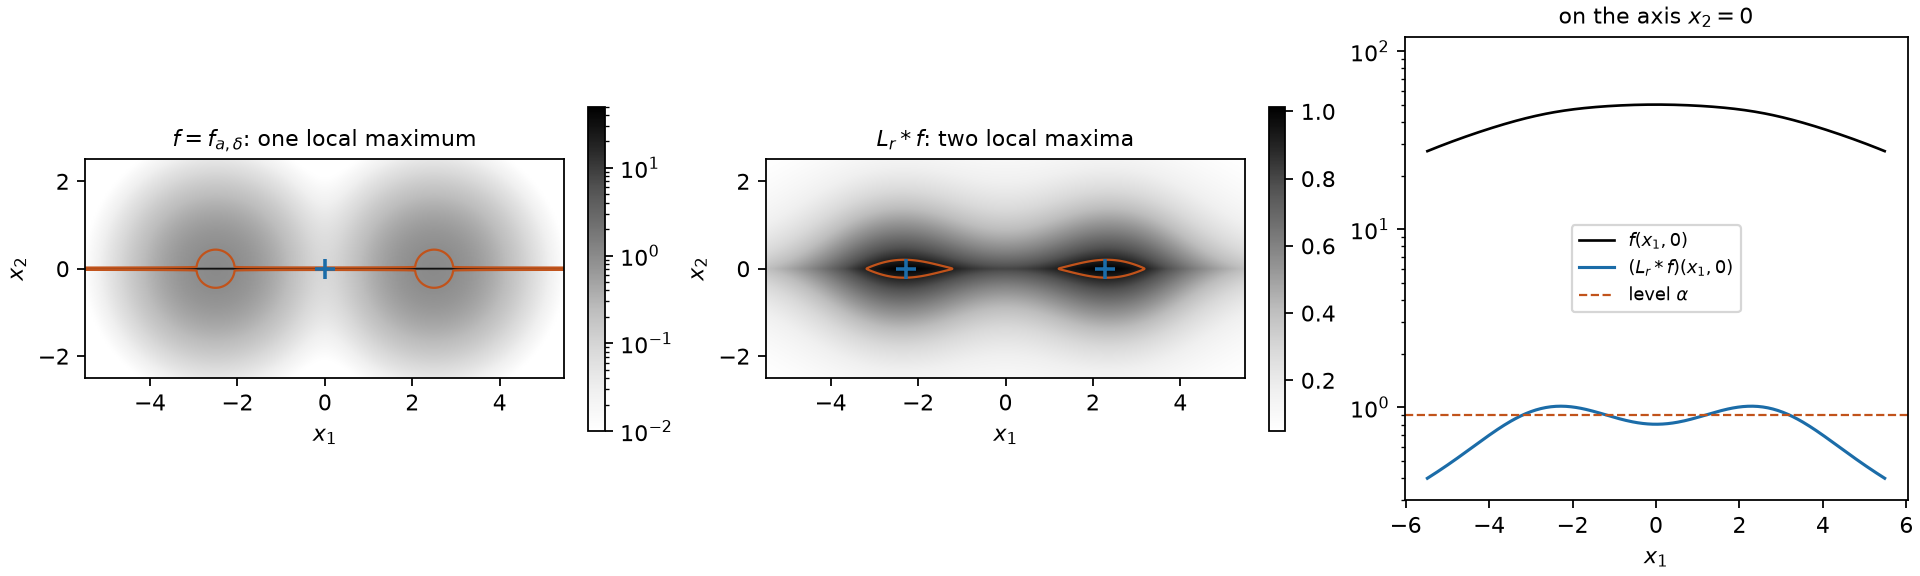
\includegraphics[width=\textwidth]{theory-creation.png}
\caption{Proposition~\ref{prop:creation-plane}(1) at $d = 2$ for the octave step $\mu = L_r$ of
the \Matern{} pyramid, $r = 1$, and the witness $f = f_{a,\delta}$ at $a = 5/2$, $\delta = 1/100$.
Left: $f$ on a logarithmic grey scale, with its one local maximum at $0$. Middle: $L_r * f$,
computed by the transform $(1 + r^2|\omega|^2)^{-1}$ on the periodic box
$[-18, 18] \times [-8, 8]$, sampled at the spacings $0.04$ along $x_1$ and $\delta/6$ along $x_2$
($900 \times 9600$ points), with two local maxima on that grid, at $(\pm2.28, 0)$. A grid point
counts as a local maximum when no neighbour of its $3 \times 3$ block is larger and its value
exceeds $10^{-3}$ of the maximum. These counts are computed. The proposition proves at least two
local maxima. The orange curves are the level $\alpha = 0.909$, midway between the value of
$L_r * f$ at $0$ and at its maxima. The set $\{f > \alpha\}$ is two discs joined by the thin strip
along the ridge, and $\{L_r * f > \alpha\}$ has two components. Right: both functions on the axis
$x_2 = 0$. By the proof of clause (3), $f$ is the record $\mu_s * g$ of the \Matern{} pyramid at
the scale $s$ with $cs = r$, so the middle panel is the next record $\mu_{qs} * g$. Let
$W := L_r * e^{-|\cdot|^2/2}$. The proof chooses a radius outside which $W < W(0)/4$, and it puts
$a$ one above that radius. Its argument needs only $a$ above the radius. Here $W = W(0)/4$ at
$2.331$, so $a = 5/2$ is admissible with any radius in $[2.331, 2.5)$. The proof's bound on the
ridge needs $\delta$ below about $0.002$, smaller than the $\delta$ drawn.}
\label{fig:theory-creation}
\end{figure}

A pyramid computed on a grid reads local maxima on the lattice, by comparing a value with the
values at finitely many neighbours. The next proposition carries the creation to that setting, in
$d \ge 2$. It covers one smoothing step by a mask. For an integer ratio $q \ge 2$ it also covers
the same step followed by decimation, and, for an infinitely divisible mask, every level of a
decimated pyramid.

% shared with blueprint prop:creation-grid
\begin{proposition}[creation on a grid]
\label{prop:creation-grid}

Let $d \ge 2$, let $w \ne \delta_0$ be a symmetric probability law on $h\ZZ^d$, and let
$\mathcal{N} \subset h\ZZ^d \setminus \{0\}$ be finite and symmetric and
contain the $2d$ axis neighbours. Call $x$ an \emph{$\mathcal{N}$-maximum} of $u$ if
$u(x) \ge u(x + y)$ for all $y \in \mathcal{N}$.
\begin{enumerate}
\item There is a summable $f > 0$ on $h\ZZ^d$ with exactly one $\mathcal{N}$-maximum such that
$w * f$ has at least two.
\item For an integer $q \ge 2$, $f$ can be chosen so that $(w * f)|_{qh\ZZ^d}$ has at least two
$q\mathcal{N}$-maxima as well.
\item If $w$ is infinitely divisible and $q \ge 2$ is an integer, then for every integer $k \ge 0$
every bounded array on $q^kh\ZZ^d$ is the level-$k$ record, smoothed and decimated $k$ times, of a bounded input on
$h\ZZ^d$: with $f_0$ the input, $f_j := \bigl((D_{q^{j-1}}w) * f_{j-1}\bigr)|_{q^jh\ZZ^d}$ and the
array $f_k$.
\end{enumerate}
\end{proposition}

\begin{proof}
Take $h = 1$, and write $|y|_1 := \sum_j|y_j|$.

\emph{An axis line of mass below one.} If every axis line $\ZZ e_j$ had mass $1$, $w$ would be
carried by their intersection $\{0\}$, as $d \ge 2$, and $w = \delta_0$. So some axis line
$\ZZ e_j$ has mass $p < 1$. The argument is written for $j = 1$; for another $j$ it is the same with
the coordinates $x_1$ and $x_j$ exchanged in the witness below, $\mathcal{N}$ entering only through
the $2d$ axis neighbours it contains. Put $\theta := 2/(1 + p)$, so that $\theta > 1$ and
$1 - \theta p = (1 - p)/(1 + p) > 0$.

\emph{The witness.} Write $x = (x_1, x')$ and $|x'|_1 := \sum_{j \ge 2}|x_j|$. Let
$\Psi(t) := \min(1 + |t|, 2e^{1 - |t|})$. It is $1 + |t|$ for $|t| \le 1$ and $2e^{1 - |t|}$
otherwise, it lies in $(0, 2]$, and $|\Psi(s) - \Psi(t)| \le 6|s - t|$. For an integer $R \ge 1$ put
\[
  b(x) := \Psi(x_1/R)\,e^{-|x'|_1/R}, \qquad
  f(x) := b(x) + \mathbf{1}_{\{x' = 0\}}\,\theta\max(1 - |x_1|/R, 0) .
\]
It is positive and even, and summable, as $f(x) \le (2 + \theta)e\,e^{-|x|_1/R}$.

\emph{One $\mathcal{N}$-maximum.} First $f(0) = 1 + \theta \ge f(x)$ for every $x$. Off the line
$f = b \le 2$. On it, $f(x) = 1 + \theta - (\theta - 1)|x_1|/R$ when $|x_1| \le R$, and $f \le 2$
beyond. So $0$ is an $\mathcal{N}$-maximum. From every $x \ne 0$ one axis step strictly raises $f$.
If $x' \ne 0$, a step toward the line in a coordinate $j \ge 2$ with $x_j \ne 0$ lowers $|x'|_1$ by
one, which raises $b$, and the ridge term cannot fall from $0$. If $x' = 0$ and $x_1 \ne 0$, the step
toward $0$ along the line raises $f$ by $(\theta - 1)/R$ while $|x_1| \le R$. Beyond, it raises $\Psi$
strictly, as $|x_1| - 1 \ge R$ (both are integers), and the ridge term is $0$ at $x$. As
$\mathcal{N}$ contains the axis neighbours, no $x \ne 0$ is an $\mathcal{N}$-maximum.

\emph{Two for the output.} The output $u := w * f$ is even, as $w$ is symmetric and $f$ even. It is
positive, and it tends to $0$ at infinity, by dominated convergence, as $f$ does. So $u$ attains its
maximum, and a maximizer is an $\mathcal{N}$-maximum for every $\mathcal{N}$. If $u(z) > u(0)$ for
some $z$, a maximizer $x^* \ne 0$ exists, and $-x^* \ne x^*$ is a second one. Now
$|b(x - y) - b(x)| \le \min(6|y|_1/R, 2)$, so
$\varepsilon(R) := \sum_yw(y)\min(6|y|_1/R, 2)$ bounds $|w * b - b|$ at every point, and
$\varepsilon(R) \to 0$ as $R \to \infty$ by dominated convergence: this is the tightness of $w$. The
ridge term of $u$ at $0$ is at most $\theta$ times the mass $p$ of the line. So
\[
  u(0) \le b(0) + \varepsilon(R) + \theta p = 1 + \varepsilon(R) + \theta p, \qquad
  u(Re_1) \ge b(Re_1) - \varepsilon(R) = 2 - \varepsilon(R),
\]
and $u(Re_1) - u(0) \ge 1 - \theta p - 2\varepsilon(R) > 0$ for large $R$. For (2), take $R = qK$
with $K$ large. Then $Re_1 = q(Ke_1)$ is on $q\ZZ^d$, and the same argument applies to the even
function $m \mapsto u(qm)$, which tends to $0$ at infinity.

\emph{(3)} Being symmetric and infinitely divisible, $w$ has \Levy{} data $(A, \nu)$ and the
generating triplet $(2A, \nu, 0)$, by Lemma~\ref{lem:symmetric-levy-khintchine}:
$\widehat w(\omega) = e^{-\langle\omega, A\omega\rangle - \int(1 - \cos\langle\omega, x\rangle)\,\nu(dx)}$.
Being carried by $\ZZ^d$, it has $A = 0$, and $\nu$ is finite and carried by
$\ZZ^d \setminus \{0\}$ (Lemma~\ref{lem:lattice-infinitely-divisible}). Put $a(n) := \nu(\{n\})$, a
summable symmetric kernel, and $M := \sum_na(n)$. Then
$\widehat w(\vartheta) = e^{-\sum_na(n)(1 - \cos\langle n, \vartheta\rangle)} = e^{-M}e^{\widehat a(\vartheta)}$,
the transform $\widehat a$ being real. Put $m := e^M\sum_{k \ge 0}(-1)^ka^{*k}/k!$. The series
converges absolutely in $\ell^1(\ZZ^d)$, with norm at most $e^{2M}$, so
$\widehat m = e^Me^{-\widehat a} = 1/\widehat w$ and $\widehat{w * m} = 1 = \widehat{\delta_0}$. A
summable kernel is determined by its Fourier coefficients, so $w * m = \delta_0$. At $k = 0$ the
array is its own input. Let $k \ge 1$, and suppose that every bounded array on $q^{k-1}\ZZ^d$ is the
level-$(k-1)$ record of a bounded input. Given a bounded array on $q^k\ZZ^d$, extend it by $0$ to a
bounded $u$ on $q^{k-1}\ZZ^d$, and put $v := (D_{q^{k-1}}m) * u$, a bounded array on
$q^{k-1}\ZZ^d$, as $D_{q^{k-1}}m$ is summable. By the induction hypothesis $v$ is the level-$(k-1)$
record $f_{k-1}$ of a bounded input $f_0$. Its smoothing $(D_{q^{k-1}}w) * v$ is
$(D_{q^{k-1}}(w * m)) * u = u$, by associativity, so
$f_k = \bigl((D_{q^{k-1}}w) * f_{k-1}\bigr)|_{q^k\ZZ^d} = u|_{q^k\ZZ^d}$ is the given array.
\end{proof}

Clause (3) carries clauses (1) and (2) to every level of a decimated grid pyramid whose mask is
infinitely divisible and whose ratio is an integer. The input that clause (1) gives for the mask at
level $k$ is bounded. So it is the level-$k$ record of a bounded input on $h\ZZ^d$, and the next
smoothing step raises the count. Section~\ref{sec:price-masks} reads the proposition on the masks of
the grid pyramids: the discrete Helmholtz mask, the frame mask and the binomial masks
(Proposition~\ref{prop:creation-grid-masks}).

\subsection{The selection}
\label{sec:matern-selection}

Counting fails in the plane, so a pyramid for images needs another principle to choose its family.
This subsection gives one, and finds the family it selects.

What remains of non-creation in the plane is non-enhancement: smoothing does not raise a local
maximum or lower a local minimum. Its classical form requires $\partial_tu \le 0$ at a spatial local
maximum of the record, which needs a derivative in scale
\prog{V-selection v0.1}{Thm.~4.2(3), p.~31}. A pyramid has no derivative in scale, only its octave
steps. Read at one finite step from $s$ to $t$, the principle requires $(u_t - u_s)/(t - s) \le 0$
at each weak local maximum of the later record $u_t$. This is the implicit Euler discretization of
the classical form. It needs no continuum of scales, so it can be required of an octave step. A
step of a family from scale $s$ to scale $t$ is its \emph{stage} $\mu_{s,t}$, and the octave step
from $t$ to $qt$ is the stage $\mu_{t,qt}$, an \emph{octave stage}.

The two forms select different families. On the line, the derivative form required at every scale
selects the Gaussian ray, the families whose exponent is $a\omega^2$,
\prog{V-selection v0.1}{Thm.~4.2(3) and Cor.~4.4, pp.~31, 33}. Among the symmetric
rotation-invariant laws, the finite-step form holds exactly for the Helmholtz resolvents
$(I - \tau\Delta)^{-1}$, $\tau \ge 0$, the identity among them. It rejects every Gaussian stage
$N(0, 2aI)$, $a > 0$ (Proposition~\ref{prop:stage-lemma}(3) and
Theorem~\ref{thm:selection-stratum-two}(4)).
\begin{itemize}
\item Definition~\ref{def:implicit-euler-principle} states the finite-step principle, on the
continuum and on a lattice.
\item The stage lemma, Proposition~\ref{prop:stage-lemma}, finds the laws that have it. Among the
symmetric rotation-invariant laws they are the Helmholtz resolvents $(I - \tau\Delta)^{-1}$,
$\tau \ge 0$.
\item The selection theorem, Theorem~\ref{thm:selection-stratum-two}, requires the principle at
every octave stage of an isotropic family covariant under $q$, in the canonical discrete gauge. It
finds the \Matern{} pyramid, up to the gauge $\chi \in \mathcal{G}_q$.
\item Proposition~\ref{prop:principle-other-readings} says what the principle gives in place of the
octave stages. Required of a kernel, for the families with transforms
$\exp\bigl(-[F(t|\omega|) - F(s|\omega|)]\bigr)$, it gives octave steps that are not resolvents.
Required of every stage, it holds for no symmetric family.
\end{itemize}

% shared with blueprint def:implicit-euler-principle
\begin{definition}[the implicit-Euler maximum principle]
\label{def:implicit-euler-principle}

A symmetric probability measure $\mu$ on $\RR^d$ has the \emph{implicit-Euler maximum principle}
if for every real $f \in \mathcal{S}(\RR^d)$ the output $u := \mu * f$ has $u(x) \le f(x)$ at every
weak local maximum $x$ of $u$, and $u(x) \ge f(x)$ at every weak local minimum. Here $x$ is a
\emph{weak local maximum} of $u$ if $u(x) \ge u(y)$ for every $y$ in a neighbourhood of $x$, and a
\emph{weak local minimum} if it is a weak local maximum of $-u$. A stage $\mu_{s,t}$ of a
family has the principle if the measure $\mu_{s,t}$ has it. On a lattice $h\ZZ^d$, with
$\mathcal{N} \subset h\ZZ^d \setminus \{0\}$ finite and symmetric, a symmetric probability $\kappa$
on $h\ZZ^d$ has the principle \emph{on $\mathcal{N}$} if for every bounded real $f$ on $h\ZZ^d$ the
output $u := \kappa * f$ has $u(x) \le f(x)$ at every $\mathcal{N}$-maximum $x$ of $u$ and
$u(x) \ge f(x)$ at every $\mathcal{N}$-minimum. Here $x$ is an \emph{$\mathcal{N}$-maximum} of $u$ if
$u(x) \ge u(x + y)$ for every $y \in \mathcal{N}$, and an \emph{$\mathcal{N}$-minimum} if it is an
$\mathcal{N}$-maximum of $-u$.
\end{definition}

The inputs are signed, so the clause at minima is the clause at maxima applied to $-f$.

The first task is to find the laws that have the principle. The answer is the stage lemma below.
On the continuum the principle holds for the resolvent of every positive semidefinite quadratic
form, and the converse shows that no symmetric probability measure on $\RR^d$ other than these
resolvents has it. On a lattice it holds for the resolvent of the $(2d+1)$-point Laplacian, read on
the $2d$ axis neighbours.

Why the principle selects the resolvents can be seen before the proof. The sufficiency is the
classical maximum principle of an elliptic equation. If
$\widehat\mu(\omega) = (1 + \omega\cdot C\omega)^{-1}$, then $u = \mu * f$ solves
$u - \nabla\cdot(C\nabla u) = f$. For a Schwartz input $u$ is smooth, since its derivatives are
$\mu * \partial^\alpha f$, whether or not $\mu$ has a bounded density. At a local maximum the
Hessian of $u$ is negative semidefinite, so $f - u = -\operatorname{tr}(C\nabla^2u) \ge 0$. The
converse tests the principle on inputs that are finite sums of cosines damped by a wide Gaussian,
chosen so that their limit outputs have a strict maximum at $0$. In the limit the principle becomes
a linear inequality on the values of $\widehat\mu$ at finitely many frequencies, with real weights of
either sign. A step of the proof shows that $\widehat\mu$ has no zero. Testing with suitable pairs of
frequencies then forces $1/\widehat\mu - 1$ to be a positive semidefinite quadratic form.

The sufficiency has a counterpart in regularization: Scherzer and Weickert read one regularization
step as one implicit diffusion step and prove its extremum principle
[\sscite{scherzer2000relations}, p.~43, and Lemma~6, p.~53]. The converse has two counterparts on
generators. An operator $A$ has the \emph{local positive maximum principle} if $Af(x) \le 0$
wherever $f$ has a local maximum $f(x) \ge 0$. A linear operator from smooth functions of compact
support to continuous functions with this principle is a second-order differential operator
[\sscite{courrege1966sur}, Thm.~0.1, p.~2-01]. Alvarez, Guichard, Lions and Morel derive a
second-order generator from a comparison principle and locality
[\sscite{alvarez1993axioms}, Thm.~2, p.~211]. The stage lemma reads its principle on one finite
step, a convolution, where these results read theirs on a generator.

% TODO(module C): cite prop:stage-lemma when released
The lemma belongs to the author's work on spatial scale space that is not yet published, so it is
stated here with its proof.

% shared with blueprint prop:stage-lemma
\begin{proposition}[the stage lemma]
\label{prop:stage-lemma}

Let $\mu$ be a symmetric probability measure on $\RR^d$.
\begin{enumerate}
\item \emph{(Sufficiency.)} For every positive semidefinite matrix $C$ there is a symmetric
probability measure with transform $(1 + \omega\cdot C\omega)^{-1}$, and it has the principle. In
particular the Helmholtz resolvent $(I - \tau\Delta)^{-1}$ has it for every $\tau \ge 0$, in every
dimension.
\item \emph{(The grid.)} On $h\ZZ^d$ the resolvent $\kappa$ of the $(2d+1)$-point Laplacian, with
transform $\bigl(1 + 4\tau h^{-2}\sum_{j=1}^d\sin^2(h\omega_j/2)\bigr)^{-1}$, $\tau \ge 0$, is a
symmetric probability and has the principle on the $2d$ axis neighbours.
\item \emph{(Converse.)} If $\mu$ has the principle, then $1/\widehat\mu(\omega) = 1 + \omega\cdot
C\omega$ for a positive semidefinite $C$. If $\mu$ is rotation invariant, $C = \tau I$ and $\mu$ is
the Helmholtz resolvent, the identity when $\tau = 0$.
\end{enumerate}
\end{proposition}

\begin{proof}
\emph{(1)} Write a positive semidefinite $C$ as $B^{\tp}B$, $B$ real, and put
$b_k := B^{\tp}e_k$, so that $\omega\cdot C\omega = |B\omega|^2 = \sum_k(\omega\cdot b_k)^2$. The
image $\mu_C$ of $L_1$ under $y \mapsto B^{\tp}y$ is a probability measure with the transform
$\widehat{L_1}(B\omega) = (1 + \omega\cdot C\omega)^{-1}$ (Lemma~\ref{lem:bessel-profile}(1)), which
is even, so $\mu_C$ is symmetric by the uniqueness of the transform.

Let $f \in \mathcal{S}(\RR^d)$ be real, and put $u := \mu_C * f$. The transform of $f$ is
$\widehat f(\omega) := \int e^{i\omega\cdot x}f(x)\,dx$, the transform of the measure $f(x)\,dx$, so
that Fourier inversion reads
$f(z) = (2\pi)^{-d}\int e^{-i\omega\cdot z}\widehat f(\omega)\,d\omega$. By Fubini's theorem $u$ has
the transform $\widehat{\mu_C}(\omega)\widehat f(\omega) =: g(\omega)$. As
$0 < \widehat{\mu_C} \le 1$ and $\widehat f$ is rapidly
decreasing, $g$ and $|\omega|^2g$ are integrable, and by Fourier inversion
\[
  u(z) = (2\pi)^{-d}\int e^{-i\omega\cdot z}g(\omega)\,d\omega, \qquad
  f(z) = (2\pi)^{-d}\int e^{-i\omega\cdot z}(1 + \omega\cdot C\omega)\,g(\omega)\,
  d\omega .
\]
These integrals are real, as $u$ and $f$ are; the real part written below only makes that
visible. So $f(x) - u(x) = (2\pi)^{-d}\sum_kQ_{b_k}$ with $Q_v := \operatorname{Re}\int e^{-i\omega\cdot x}
(\omega\cdot v)^2g(\omega)\,d\omega$. For a vector $v$ and $s \ne 0$,
\[
  \frac{u(x + sv) + u(x - sv) - 2u(x)}{s^2} = (2\pi)^{-d}\operatorname{Re}\int e^{-i\omega\cdot x}\,
  \frac{2\cos(s\,\omega\cdot v) - 2}{s^2}\,g(\omega)\,d\omega .
\]
The fraction in the integrand tends to $-(\omega\cdot v)^2$ as $s \to 0$ and is bounded by
$(\omega\cdot v)^2 \le |v|^2|\omega|^2$, as $1 - \cos y \le y^2/2$, so by dominated convergence the
quotient tends to $-(2\pi)^{-d}Q_v$. At a local maximum $x$ of $u$ its numerator is $\le 0$ for
small $s$, so $Q_v \ge 0$ for every $v$, and $f(x) \ge u(x)$. Minima follow with $-f$. The
Helmholtz resolvent is $C = \tau I$.

\emph{(2)} At $\tau = 0$, $\kappa = \delta_0$. Let $\tau > 0$, put $a := \tau h^{-2}$ and
$p := 2da/(1 + 2da) \in (0, 1)$, and let $\sigma$ be the simple random walk step, of mass $1/(2d)$ at
each $\pm he_j$, with transform $\widehat\sigma(\omega) = d^{-1}\sum_j\cos(h\omega_j)$. The
measure $(1 - p)\sum_{k \ge 0}p^k\sigma^{*k}$ is a symmetric probability on $h\ZZ^d$, a convex
combination of such, with the transform $(1 - p)/(1 - p\widehat\sigma)$. Its reciprocal is
$1 + \frac{p}{1 - p}(1 - \widehat\sigma) = 1 + 2da\cdot d^{-1}\sum_j(1 - \cos h\omega_j) =
1 + 4\tau h^{-2}\sum_j\sin^2(h\omega_j/2)$. So it is $\kappa$, by the uniqueness of Fourier
coefficients.
Let $\Delta_hu(n) := h^{-2}\sum_j\bigl(u(n + he_j) - 2u(n) + u(n - he_j)\bigr)$. The series gives
$\kappa * \sigma = (\kappa - (1 - p)\delta_0)/p$, and $\Delta_h\kappa = 2dh^{-2}(\kappa * \sigma -
\kappa)$, so $\kappa - \tau\Delta_h\kappa = \delta_0$, since $(1 - p)(1 + 2da) = 1$. For bounded real
$f$, $u := \kappa * f$ is bounded and $\Delta_hu = (\Delta_h\kappa) * f$, by shifting the summation
index, $\kappa$ being summable. So $u - \tau\Delta_hu = f$. At a maximum $x$ of $u$ over the axis
neighbours every term $u(x \pm he_j) - u(x)$ is nonpositive, so $\Delta_hu(x) \le 0$ and
$f(x) \ge u(x)$. Minima follow with $-f$.

\emph{(3)}
Write $\rho := \widehat\mu$. It is real, since $\mu$ is symmetric, continuous, and $\rho(0) = 1$.
The sine integrates to $0$ against $\mu$, so for $w, x \in \RR^d$
\[
  \int\cos\langle w, x - y\rangle\,\mu(dy) = \rho(w)\cos\langle w, x\rangle .
\]
The principle is tested on the inputs $\sum_ka_k\cos\langle w_k, x\rangle e^{-s|x|^2}$, whose
outputs tend as $s \to 0$ to $\sum_ka_k\rho(w_k)\cos\langle w_k, x\rangle$. Step~1 turns it into an
inequality between finitely many values of $\rho$, Step~2 shows that $\rho$ has no zero, and
Step~3 that $1/\rho - 1$ is a nonnegative quadratic form.

\emph{Step 1: the inequality.} Let $a_1, \dots, a_n \in \RR$ and $w_1, \dots, w_n \in \RR^d$, put
$b_k := a_k\rho(w_k)$, and suppose that $\sum_kb_k\langle w_k, x\rangle^2 \ge c|x|^2$ for every $x$,
with $c > 0$. Then $\sum_kb_k \le \sum_ka_k$. Step~2 applies this to pairs $(a_k, w_k)$ of a
weight and a frequency.

For $s \in (0, 1]$ the input $f_s(x) := \sum_ka_k\cos\langle w_k, x\rangle\,e^{-s|x|^2}$ is a real
Schwartz function, a Gaussian times functions whose derivatives are all bounded. Put
$h(x) := \sum_kb_k\cos\langle w_k, x\rangle$ and $A := \sum_k|a_k|$. By the identity above, and as
$|x - y| \le 1 + |y|$ for $|x| \le 1$,
\[
  \bigl|(\mu * f_s)(x) - h(x)\bigr| \le A\int\bigl(1 - e^{-s|x - y|^2}\bigr)\,\mu(dy)
  \le A\int\bigl(1 - e^{-s(1 + |y|)^2}\bigr)\,\mu(dy) \qquad (|x| \le 1),
\]
and the right side tends to $0$ as $s \to 0$, by dominated convergence. Next, $|\cos y - 1 +
y^2/2| \le y^4$ for $|y| \le 1$. With $K := \sum_k|b_k||w_k|^4$, as long as $|x||w_k| \le 1$ for
every $k$,
\[
  h(x) \le h(0) - \tfrac12\sum_kb_k\langle w_k, x\rangle^2 + K|x|^4
  \le h(0) - \tfrac c2|x|^2 + K|x|^4 ,
\]
so there is $r_0 \in (0, 1]$ with $h(x) \le h(0) - \frac c4|x|^2$ for $|x| \le r_0$. Let
$0 < r \le r_0$, and choose $s \in (0, 1]$ with $|\mu * f_s - h| < cr^2/8$ on the unit ball. The output
$u := \mu * f_s$ is continuous, so it attains its maximum over the closed ball of radius $r$ at some
point $x_s$. On the sphere $|x| = r$, $u(x) < h(x) + cr^2/8 \le h(0) - cr^2/8 < u(0)$, so
$|x_s| < r$, and $x_s$ is a local maximum of $u$. The principle gives
$h(0) - cr^2/8 < u(0) \le u(x_s) \le f_s(x_s)$. From $1 - y^2/2 \le \cos y \le 1$ and
$1 - e^{-t} \le t$, $f_s(x) \le \sum_ka_k + A_1|x|^2$ with $A_1 := \sum_k|a_k|(|w_k|^2/2 + 1)$.
Hence $\sum_kb_k = h(0) < \sum_ka_k + (A_1 + c/8)r^2$ for every $r \in (0, r_0]$, and
$\sum_kb_k \le \sum_ka_k$.

\emph{Step 2: $\rho$ has no zero.} By continuity there is $t > 0$ with $\rho(te_i) \ge \frac12$ for
$i = 1, \dots, d$. Suppose $\rho(\omega_0) = 0$, and apply Step~1 to the pairs $(1, te_i)$,
$i = 1, \dots, d$, and $(a_0, \omega_0)$. Whatever $a_0$, the hypothesis holds with $c = t^2/2$,
since $b_0 = a_0\rho(\omega_0) = 0$. The conclusion $\sum_i\rho(te_i) \le d + a_0$ fails for
$a_0 = -d - 1$.

\emph{Step 3: the reciprocal.} Put $m := 1/\rho - 1$. Step~1 with $a_k := b_k/\rho(w_k)$ reads: if
$\sum_kb_k\langle w_k, x\rangle^2 \ge c|x|^2$ for every $x$, with $c > 0$, then
$\sum_kb_km(w_k) \ge 0$. In the rest of this step a pair $(b_k, w_k)$ names the weight $b_k$ of this
form, not the weight $a_k$ of Step~1. If instead $\sum_kb_k\langle w_k, x\rangle^2 = 0$ for every $x$, the pairs
$(b_k, w_k)$ together with $(\varepsilon, e_i)$, $i = 1, \dots, d$, have the form $\varepsilon|x|^2$,
so $\sum_kb_km(w_k) + \varepsilon\sum_im(e_i) \ge 0$ for every $\varepsilon > 0$. The same holds
for $-b$, so $\sum_kb_km(w_k) = 0$. In the same way the pairs $(1, \omega)$ and
$(\varepsilon, e_i)$ give $m(\omega) \ge 0$. Let $C_{ij} := \frac12\bigl(m(e_i + e_j) - m(e_i) -
m(e_j)\bigr)$, a symmetric matrix. Fix $\omega$. The pair $(1, \omega)$ and, for all $i$ and $j$,
the pairs $(-\omega_i\omega_j/2, e_i + e_j)$, $(\omega_i\omega_j/2, e_i)$ and
$(\omega_i\omega_j/2, e_j)$ have the form $\langle\omega, x\rangle^2 -
\sum_{i,j}\omega_i\omega_jx_ix_j = 0$. So
$m(\omega) = \sum_{i,j}C_{ij}\omega_i\omega_j = \omega\cdot C\omega$. This is $\ge 0$ for every
$\omega$, so $C$ is positive semidefinite, and $1/\widehat\mu(\omega) = 1 + \omega\cdot C\omega$.

\emph{Rotation invariance.} If $\mu$ is rotation invariant, $\widehat\mu$ is radial, so
$\omega\cdot C\omega = \tau|\omega|^2$ with $\tau := e_1\cdot Ce_1 \ge 0$, and
$\widehat\mu(\omega) = (1 + \tau|\omega|^2)^{-1}$: $\mu$ is the Helmholtz resolvent. Any positive
semidefinite $C'$ with $1/\widehat\mu(\omega) = 1 + \omega\cdot C'\omega$ has the quadratic form
$\tau|\omega|^2$, so $C' = \tau I$, a symmetric matrix being determined by its quadratic form. When
$\tau = 0$, $\widehat\mu = 1$ and $\mu = \delta_0$, by the uniqueness of the transform.
\end{proof}

So a symmetric, rotation-invariant probability measure has the principle if and only if it is a
Helmholtz resolvent $(I - \tau\Delta)^{-1}$, $\tau \ge 0$. The converse assumes no infinite
divisibility and no other class of laws.

The lemma is about one law, and a pyramid has a whole ladder of octave stages. Between its knots a
family covariant under $q$ is in general not determined by its ladder, not even up to a relabelling
of the scales (Proposition~\ref{prop:ladder-knot-kernel}(2)). So the question is how much of a
family the principle fixes when it is required of its octave stages. The next theorem answers it
for an isotropic $q$-covariant family in the canonical discrete gauge. Required of one octave stage,
the principle fixes the ladder through it, and the stages between the rungs stay free. Required at
every octave stage $\mu_{t,qt}$, $t \in [1, q)$, it fixes the family up to the gauge
$\chi \in \mathcal{G}_q$, and full covariance follows. The last two clauses say which stages of the
\Matern{} pyramid have the principle. They also show that the Gaussian stages fail it, and so, in
$d \ge 2$, does the octave step of the frame \Matern{} pyramid.

% shared with blueprint thm:selection-stratum-two
\begin{theorem}[the selection, inside stratum 2]
\label{thm:selection-stratum-two}

Let $(\mu_{s,t})$ be an isotropic $q$-covariant family in dimension $d$, in the canonical discrete
gauge, with exponents $\Psi_t(|\omega|) := -\log\widehat{\mu_t}(\omega)$. Write $F^1_q$ for $F_q$ at
$c = 1$.
\begin{enumerate}
\item \emph{(One stage.)} For one $t > 0$, $\mu_{t,qt}$ has the principle if and only if
$\Psi_t(r) = \sum_{n \ge 1}\log(1 + \tau q^{-2n}r^2)$ for some $\tau > 0$. Then the whole ladder
through $t$ is that of the \Matern{} pyramid, $\mu_{q^kt,q^{k+1}t} = L_{\sqrt\tau q^k}$ for
$k \in \ZZ$, and the stages between the rungs are free: the isotropic $q$-covariant families in
the canonical discrete gauge with this ladder are not unique, and not unique up to a relabelling in
$\mathcal{G}_q$ either.
\item \emph{(Every octave stage.)} If $\mu_{t,qt}$ has the principle for all $t \in [1, q)$, then
there is $\chi \in \mathcal{G}_q$ with $\Psi_t = F^1_q(\chi(t)\,\cdot)$. So the family is the
\Matern{} pyramid of Theorem~\ref{thm:matern-pyramid} read in the gauge $\chi$, and it is fully
covariant, with $S_\lambda = \chi^{-1}(\lambda\chi)$. Conversely every such family has the
property.
\item \emph{(Which stages.)} Let $(\mu^{\mathrm M}_{s,t})$ be the \Matern{} pyramid of
Theorem~\ref{thm:matern-pyramid} with the constants $q$ and $c > 0$. Its stage
$\mu^{\mathrm M}_{s,t}$ with $0 < s < t$ has the principle if and only if $t = qs$, and
$\mu^{\mathrm M}_{0,t}$ with $t > 0$ never has it. In particular two octaves together fail, as does every stage
between other scales.
\item \emph{(Not selected.)} Let $c > 0$ and $t > 0$. A Gaussian stage $N(0, 2aI)$, $a > 0$, fails
the principle. The octave step at $t$ of the frame \Matern{} pyramid with the constant $c$
(Definition~\ref{def:frame-matern-pyramid}),
$\prod_j(1 + c^2t^2\omega_j^2)^{-1}$, fails it in $d \ge 2$, on the continuum, while each of its
axis passes has it.
\end{enumerate}
\end{theorem}

The proof of clause (2) recovers the gauge from the stages. At each starting scale $t$, clause (1)
gives the stage as $L_{\sqrt{\tau}}$ for a constant $\tau = \tau(t) > 0$, and
$\widehat{\mu_t}(\omega) = \exp(-F^1_q(\sqrt{\tau(t)}\,|\omega|))$. Covariance under $q$ gives
$\chi(qt) = q\chi(t)$ for $\chi := \sqrt\tau$. The cascade and (ND) make $\chi$ strictly increasing,
and continuity in scale makes it continuous. With $\chi(q^nt) = q^n\chi(t)$ it then maps
$(0, \infty)$ onto itself, so $\chi$ lies in $\mathcal{G}_q$.

\begin{proof}
\emph{(1)} The stage $\mu_{t,qt}$ is rotation invariant by (I3), and symmetric, $-I$ being
orthogonal, so Proposition~\ref{prop:stage-lemma}(3) gives
$\widehat{\mu_{t,qt}}(\omega) = (1 + \tau|\omega|^2)^{-1}$ with $\tau \ge 0$; and $\tau > 0$ by
(ND), as $\tau = 0$ makes $\mu_{t,qt} = \delta_0$. In the canonical discrete gauge
$D_q\mu_{0,t} = \mu_{0,qt}$, and $\mu_{0,qt} = \mu_{t,qt} * \mu_{0,t}$ by (I1), so
$\widehat{\mu_t}(q\omega) = (1 + \tau|\omega|^2)^{-1}\,\widehat{\mu_t}(\omega)$. Applied at
$q^{-n}\omega$, $n = 1, \dots, N$, this gives
\[
  \widehat{\mu_t}(\omega) = \widehat{\mu_t}(q^{-N}\omega)\prod_{n=1}^N
    \bigl(1 + \tau q^{-2n}|\omega|^2\bigr)^{-1} ,
\]
and $\widehat{\mu_t}(q^{-N}\omega) \to \widehat{\mu_t}(0) = 1$, as $\widehat{\mu_t}$ is
continuous. The product tends to $\exp\bigl(-\sum_{n \ge 1}\log(1 + \tau q^{-2n}|\omega|^2)\bigr)$,
the series converging since $\log(1 + x) \le x$. This is the form of $\Psi_t$, read on the
transform. Conversely, if $\Psi_t$ has that form, the series is $F^1_q(\sqrt\tau\,|\omega|)$, and
the telescoping $F^1_q(qr) = \log(1 + r^2) + F^1_q(r)$ gives
$\widehat{\mu_{t,qt}}(\omega) = \widehat{\mu_t}(q\omega)/\widehat{\mu_t}(\omega) =
(1 + \tau|\omega|^2)^{-1}$. So $\mu_{t,qt} = L_{\sqrt\tau}$ by Lemma~\ref{lem:bessel-profile}(1)
and the uniqueness of the transform, and it has the principle by
Proposition~\ref{prop:stage-lemma}(1). The stage at $q^kt$, $k \in \ZZ$, is the dilate
$D_{q^k}L_{\sqrt\tau} = L_{\sqrt\tau q^k}$, by covariance applied $|k|$ times.

For the freedom between the rungs it suffices to take $t = 1$. If $(\mu'_{s,u})$ is an isotropic
$q$-covariant family with $S_qu = qu$ and the steps $\mu'_{q^k,q^{k+1}} = L_{\sqrt\tau q^k}$,
$k \in \ZZ$, then $(\mu'_{s/t,u/t})$ is one with the ladder through $t$ of (1). A relabelling by
$g \in \mathcal{G}_q$ between two families so rescaled is a relabelling by
$u \mapsto g(tu)/t$, again in $\mathcal{G}_q$, between the families before rescaling. So it
suffices to build two isotropic families with $S_qu = qu$ and the ladder $(L_{\sqrt\tau q^k})_k$
that are not relabellings of each other by any element of $\mathcal{G}_q$.
Proposition~\ref{prop:ladder-knot-kernel}(2) gives them for the step $\varrho := L_{\sqrt\tau}$.

Let $\nu$ be the measure with the radial density
$b_d(|x|/\sqrt\tau)\bigl(|S^{d-1}|\,|x|^d\bigr)^{-1}$. By Lemma~\ref{lem:bessel-profile}(2) at
$\beta = \tau$, $\int(1 - \cos\langle\omega, x\rangle)\,\nu(dx) = \log(1 + \tau|\omega|^2)$.
In polar coordinates $\int(1 \wedge |x|^2)\,\nu(dx) = \int_0^\infty(1 \wedge r^2)\,b_d(r/\sqrt\tau)\,dr/r$,
which is finite since $b_d \le 2$ and $b_d(y) \le C_de^{-y/2}$ (Lemma~\ref{lem:bessel-profile}(3)).
So $\nu$ is a rotation-invariant \Levy{} measure, and the infinitely divisible law with the data
$(0, \nu)$ has the transform $(1 + \tau|\omega|^2)^{-1}$. It is $\varrho$, by
Lemma~\ref{lem:bessel-profile}(1), so $\varrho$ is symmetric, rotation invariant, infinitely
divisible and not $\delta_0$. Its logarithmic moment is finite, since $\log_+ r \le r$ and so
$\log_+ r\,b_d(r/\sqrt\tau)/r \le C_d e^{-r/(2\sqrt\tau)}$. Split $\nu = \nu_a + \nu_b$, with
$\nu_a$ the restriction of $\nu$ to $\{|x| \le 1\}$ and $\nu_b$ its restriction to $\{|x| > 1\}$.
Both are symmetric and rotation invariant, carried by disjoint sets, and nonzero since $b_d > 0$.
By Proposition~\ref{prop:ladder-knot-kernel}(2) there are two isotropic $q$-covariant families
with $S_qu = qu$ and the step $\mu_{1,q} = \varrho$, neither a relabelling of the other by an
element of $\mathcal{G}_q$. Covariance gives their ladder,
$\mu_{q^k,q^{k+1}} = D_{q^k}L_{\sqrt\tau} = L_{\sqrt\tau q^k}$. This is the last sentence of (1).

\emph{(2)} Every stage $\mu_{t,qt}$, $t > 0$, has the principle. With $q^nt \in [1, q)$, clause (1)
makes the stage at $q^nt$ the law $L_{\sqrt\tau}$, and the stage at $t$ is its dilate
$L_{\sqrt\tau q^{-n}}$, which has the principle by Proposition~\ref{prop:stage-lemma}(1). So clause
(1) applies at every $t > 0$: $\widehat{\mu_t}(\omega) = \exp(-F^1_q(\chi(t)|\omega|))$ with
$\chi(t) := \sqrt{\tau(t)} > 0$, since $\sum_n\log(1 + \tau q^{-2n}r^2) = F^1_q(\sqrt\tau r)$. As
$F^1_q$ is strictly increasing on $[0, \infty)$, $\chi(t)$ is read off $\widehat{\mu_t}(e)$ at a
unit vector $e$, and covariance, $D_{q^n}\mu_{0,t} = \mu_{0,q^nt}$, gives
$\chi(q^nt) = q^n\chi(t)$ for $n \in \ZZ$. If $\chi(t) \le \chi(s)$ with $s < t$, then by (I1)
$\widehat{\mu_{s,t}}(\omega) = \exp\bigl(F^1_q(\chi(s)|\omega|) - F^1_q(\chi(t)|\omega|)\bigr) \ge 1$.
A transform has modulus at most $1$, so $\widehat{\mu_{s,t}} = 1$ and $\mu_{s,t} = \delta_0$,
against (ND). So $\chi$ is strictly increasing on $(0, \infty)$. It is continuous there:
$\exp(-F^1_q(\chi(t))) = \widehat{\mu_t}(e)$ is continuous in $t$ by (I2), and if
$a' > \chi(t_0)$, then $F^1_q(a') > F^1_q(\chi(t_0))$, so $\chi(t) < a'$ for $t$ near $t_0$;
likewise from below. By the intermediate values $\chi([1, q]) \supseteq [\chi(1), q\chi(1)]$, and
with the dilations $\chi$ maps $(0, \infty)$ onto itself. So $\chi \in \mathcal{G}_q$, with
$\chi(0) := 0$. By (I1) the transforms are those of Theorem~\ref{thm:matern-pyramid} at $c = 1$ in
the gauge $\chi$,
$\widehat{\mu_{s,t}}(\omega) = \exp\bigl(-[F^1_q(\chi(t)|\omega|) - F^1_q(\chi(s)|\omega|)]\bigr)$,
and the transform determines the law. The map $S_\lambda := \chi^{-1}(\lambda\chi)$, with
$S_\lambda(0) := 0$, is an increasing bijection of $[0, \infty)$, and reading the transforms at
$\lambda\omega$ gives $D_\lambda\mu_{s,t} = \mu_{S_\lambda s, S_\lambda t}$ for every
$\lambda > 0$. Conversely, for such a family telescoping gives
$\widehat{\mu_{t,qt}}(\omega) = (1 + \chi(t)^2|\omega|^2)^{-1}$, so $\mu_{t,qt} = L_{\chi(t)}$ by
Lemma~\ref{lem:bessel-profile}(1) and the uniqueness of the transform, and
Proposition~\ref{prop:stage-lemma}(1) applies.

\emph{(3)} The stage $\mu^{\mathrm M}_{s,t}$, $0 \le s < t$, has the transform
$\exp\bigl(-[F_q(t|\omega|) - F_q(s|\omega|)]\bigr)$, real and even, so it is symmetric. If it
has the principle, Proposition~\ref{prop:stage-lemma}(3) along a unit vector $e$ gives
$\exp D(x) = 1 + kx^2$ for $x \ge 0$, with $D(x) := F_q(tx) - F_q(sx)$ and
$k := e\cdot Ce \ge 0$. The telescoping $F_q(qy) = \log(1 + c^2y^2) + F_q(y)$ at $y = tx$ and
$y = sx$ gives $D(qx) = D(x) + \log(1 + c^2t^2x^2) - \log(1 + c^2s^2x^2)$, so with $u = x^2$
\[
  (1 + kq^2u)(1 + c^2s^2u) = (1 + c^2t^2u)(1 + ku) , \qquad u \ge 0 .
\]
Both sides are polynomials in $u$ of degree at most $2$ with the constant term $1$, so their equality at $u = 1$ and $u = 2$ makes the coefficients of $u^2$ and of $u$ agree:
$kc^2(t^2 - q^2s^2) = 0$ and $c^2(t^2 - s^2) = k(q^2 - 1)$. If $k = 0$, the second gives $t = s$,
which is excluded; so $k > 0$, and the first gives $t = qs$. At $s = 0$ this reads $t = 0$, which is
excluded: $\mu^{\mathrm M}_{0,t}$ never has the principle. Conversely
$\mu^{\mathrm M}_{s,qs} = L_{cs}$ (Theorem~\ref{thm:matern-pyramid}(1)) has the principle by
Proposition~\ref{prop:stage-lemma}(1).

\emph{(4)} The Gaussian stage and the frame step have real even transforms, so they are symmetric.
If the Gaussian stage had the principle, Proposition~\ref{prop:stage-lemma}(3) along a unit vector
would give $e^{ax^2} = 1 + kx^2$ for every $x$; at $x = 1$ and $x = \sqrt2$,
$(1 + k)^2 = e^{2a} = 1 + 2k$, so $k = 0$ and $a = 0$, which is excluded. If the frame step had it,
the same proposition would give $\prod_j(1 + c^2t^2\omega_j^2) = 1 + \omega\cdot C\omega$. On the
diagonal $\omega = x(e_1 + e_2)$, which $d \ge 2$ allows, this reads
$(1 + Kx^2)^2 = 1 + Qx^2$ with $K := c^2t^2 > 0$ and $Q := (e_1 + e_2)\cdot C(e_1 + e_2)$; at
$x = 1$ and $x = \sqrt2$ it gives $2K^2 = 0$, which is excluded. The axis pass along $e_j$, the
Laplace law on the line $\RR e_j$ with transform $(1 + c^2t^2\omega_j^2)^{-1}$, is
Proposition~\ref{prop:stage-lemma}(1) with the degenerate $C = c^2t^2e_je_j^{\tp}$.
\end{proof}

Clause (4) is stated on the continuum. Its grid case is in Section~\ref{sec:price-obstruction}. On
$h\ZZ^d$, $d \ge 2$, the frame mask, which is the octave step of the frame \Matern{} pyramid on the
grid, fails the principle on every finite symmetric neighbourhood. Each of its axis passes has it on
every such neighbourhood that contains the two neighbours along its axis
(Proposition~\ref{prop:grid-frame-step-not-selected}).

A heuristic picture shows why a Gaussian stage fails. The proof of clause (4) does not use it. Take
a nonnegative input with two narrow bumps at $\pm be_1$ and nothing between them. A kernel with a
$C^2$ density and a nondegenerate maximum at $0$ merges them into one maximum at the origin, when
$b$ is small against its width and the bumps are narrow against $b$. There the output is positive
and the input is zero, so $u > f$ at a maximum. The Gaussian is such a kernel. The resolvent's
kernel is not smooth at its centre. It has a corner on the line and a singularity in the plane
(Proposition~\ref{prop:matern-generator-octave}(3)), so the picture does not apply to it. That the
resolvent passes is clause (1) of Proposition~\ref{prop:stage-lemma}.

In the plane, then, the case for the \Matern{} pyramid rests on non-enhancement read at a finite
step, through the converse of the stage lemma. Counting fails on the \Matern{} and frame \Matern{}
ladders, and at every rung of the Gaussian ladder (Section~\ref{sec:matern-counting}). It survives on
the projections of Theorem~\ref{thm:matern-pyramid}(3), for inputs whose projection has a version
that is the primitive of an integrable function. On a grid the resolvent of the $(2d+1)$-point
Laplacian has the principle on the $2d$ axis neighbours (Proposition~\ref{prop:stage-lemma}(2)).
The frame mask lacks it on every finite symmetric neighbourhood
(Proposition~\ref{prop:grid-frame-step-not-selected}).

The selection theorem requires the principle of the octave stages, and this is a choice. Two other
readings suggest themselves. The first requires it of the kernels $\mu_{0,t}$, read from the
origin. The second requires it of every stage. The next proposition shows that neither gives a
pyramid whose octave steps are resolvents. Its first clause covers the families with transforms
$\exp\bigl(-[F(t|\omega|) - F(s|\omega|)]\bigr)$, and its second every symmetric family.

% shared with blueprint prop:principle-other-readings
\begin{proposition}[the principle read from the origin and at every stage]
\label{prop:principle-other-readings}

Let $d \ge 1$.
\begin{enumerate}
\item \emph{(From the origin.)} Let $F$ be a real function on $[0, \infty)$ with $F(0) = 0$, not
identically $0$, and let
$(\mu_{s,t})$ be a family in dimension $d$ with
$\widehat{\mu_{s,t}}(\omega) = \exp\bigl(-[F(t|\omega|) - F(s|\omega|)]\bigr)$. If the kernel
$\mu_{0,t}$ has the principle for one $t > 0$, then $F(r) = \log(1 + \tau r^2)$ for some
$\tau > 0$, the \Matern{} family of index $1$, and then every kernel $\mu_{0,t}$ has it. Its octave
steps, with transform $(1 + \tau t^2|\omega|^2)/(1 + \tau q^2t^2|\omega|^2)$ for a ratio $q > 1$, are
not resolvents $(1 + \omega\cdot C\omega)^{-1}$.
\item \emph{(Every stage.)} No symmetric family in dimension $d$ has the principle at every stage
$\mu_{s,t}$, $0 \le s < t$.
\end{enumerate}
\end{proposition}

\begin{proof}
\emph{(1)} The kernel $\mu_{0,t}$ has the transform $e^{-F(t|\omega|)}$, as $F(0) = 0$, which is
real and even, so $\mu_{0,t}$ is symmetric. By Proposition~\ref{prop:stage-lemma}(3),
$1/\widehat{\mu_{0,t}}(\omega) = 1 + \omega\cdot C\omega$ with $C$ positive semidefinite. Along a
unit vector $e$, with $k := e\cdot Ce \ge 0$, this reads $e^{F(tx)} = 1 + kx^2$ for $x \ge 0$, so
$F(r) = \log(1 + \tau r^2)$ for $r \ge 0$, with $\tau := k/t^2 \ge 0$, and $\tau > 0$ as $F$ is not
identically $0$. Then $\widehat{\mu_{0,t'}}(\omega) = (1 + \tau t'^2|\omega|^2)^{-1}$ for every
$t' > 0$, which has the principle by Proposition~\ref{prop:stage-lemma}(1). Suppose the octave
step $\mu_{t',qt'}$, with transform $(1 + \tau t'^2|\omega|^2)/(1 + \tau q^2t'^2|\omega|^2)$, were
$(1 + \omega\cdot C'\omega)^{-1}$ for a real matrix $C'$. Along $e$, with $a := \tau t'^2 > 0$ and
$K := e\cdot C'e$, $(1 + ax^2)(1 + Kx^2) = 1 + aq^2x^2$ for $x \ge 0$. At $x = 1$ and $x = \sqrt2$
this gives $a + K + aK = aq^2$ and $2a + 2K + 4aK = 2aq^2$, so $aK = 0$, hence $K = 0$, and then
$a = aq^2$, $q = 1$, a contradiction.

\emph{(2)} Suppose every stage has the principle. By Proposition~\ref{prop:stage-lemma}(3) there
are positive semidefinite $C_1$, $C_2$, $C_3$ with
$1/\widehat{\mu_{0,1}} = 1 + \omega\cdot C_1\omega$, $1/\widehat{\mu_{1,2}} = 1 + \omega\cdot
C_2\omega$ and $1/\widehat{\mu_{0,2}} = 1 + \omega\cdot C_3\omega$. Write
$Q_i(\omega) := \omega\cdot C_i\omega \ge 0$. The cascade $\mu_{0,2} = \mu_{1,2} * \mu_{0,1}$,
read at $x\omega$, gives $(1 + x^2Q_1(\omega))(1 + x^2Q_2(\omega)) = 1 + x^2Q_3(\omega)$, and at
$x = 1$ and $x = \sqrt2$, as in (1), $Q_1(\omega)Q_2(\omega) = 0$ for every $\omega$. Write
$C_i = B_i^\top B_i$, so that $Q_i(\omega) = |B_i\omega|^2$ and a zero of $Q_i$ is in the kernel of
$B_i$. If $Q_1(\omega_1) > 0$ and $Q_2(\omega_2) > 0$, then $Q_2(\omega_1) = 0 = Q_1(\omega_2)$, so
$Q_1(\omega_1 + \omega_2) = Q_1(\omega_1) > 0$ and $Q_2(\omega_1 + \omega_2) = Q_2(\omega_2) > 0$,
against the product's vanishing at $\omega_1 + \omega_2$. So $Q_1 \equiv 0$ or $Q_2 \equiv 0$: then
$\widehat{\mu_{0,1}} \equiv 1$ or $\widehat{\mu_{1,2}} \equiv 1$, that is $\mu_{0,1} = \delta_0$ or
$\mu_{1,2} = \delta_0$, against (ND).
\end{proof}

Read from the origin, among the families with transforms
$\exp\bigl(-[F(t|\omega|) - F(s|\omega|)]\bigr)$, the principle selects one whose octave steps are
not resolvents. Read at every stage, it is satisfied by no symmetric family. Of the three readings, the ladder is the one under which
the octave steps are Helmholtz resolvents, and Theorem~\ref{thm:selection-stratum-two} takes it.

The principle bounds the value of the output at a weak local maximum by the input there. It says
nothing about the number of local maxima. The resolvent $L_{ct}$ has the principle and still
creates local maxima (Proposition~\ref{prop:creation-plane}(1)). On a grid the principle is proved
here for one smoothing step (Proposition~\ref{prop:stage-lemma}(2)). A pyramid decimates after
each step, and a local maximum of a decimated record need not be a local maximum on the finer grid.
For the $(2d+1)$-point resolvent and one finitely supported input, the inequality of the principle
fails at a maximum of the decimated output over its axis neighbours on the coarse grid.

% shared with blueprint prop:principle-after-decimation
\begin{proposition}[the pointwise principle after decimation]
\label{prop:principle-after-decimation}

Let $d \ge 1$, $h > 0$ and $\tau > 0$, let $\kappa$ be the resolvent of
Proposition~\ref{prop:stage-lemma}(2) on $h\ZZ^d$, and let $\Delta_h$ be the $(2d+1)$-point
Laplacian, $\Delta_hu(x) := h^{-2}\sum_{j=1}^d\bigl(u(x + he_j) - 2u(x) + u(x - he_j)\bigr)$. Let
$u(0) := 1$, $u(\pm he_j) := 2$ for $j = 1, \dots, d$, and $u := 0$ elsewhere on $h\ZZ^d$, and put
$f := u - \tau\Delta_hu$.
\begin{enumerate}
\item $\kappa * f = u$, and $f(0) = 1 - 2d\tau/h^2 < u(0)$.
\item \emph{(After decimation.)} For every integer $q \ge 2$, $u$ vanishes at the $2d$ axis
neighbours $\pm qhe_j$ of the origin in the coarse grid $qh\ZZ^d$, so the origin is a strict
maximum of $u$ restricted to $qh\ZZ^d$ over those neighbours, while $u(0) > f(0)$. The decimated
output and the decimated input, $u$ and $f$ restricted to $qh\ZZ^d$, fail the inequality
$u(x) \le f(x)$ of Definition~\ref{def:implicit-euler-principle} at that maximum.
\item \emph{(Before decimation.)} On $h\ZZ^d$ the origin is not a maximum of $u$ over its axis
neighbours, and the pair $(u, f)$ satisfies the principle on the $2d$ axis neighbours at every
point of $h\ZZ^d$, by Proposition~\ref{prop:stage-lemma}(2).
\end{enumerate}
\end{proposition}

\begin{proof}
\emph{(1)} First, $\kappa - \tau\Delta_h\kappa = \delta_0$. Both sides are summable on $h\ZZ^d$,
the transform of the left side is
$\bigl(1 + 4\tau h^{-2}\sum_{j=1}^d\sin^2(h\omega_j/2)\bigr)\widehat\kappa(\omega) = 1$, and a
summable function on $h\ZZ^d$ is determined by its transform. The function $u$ has finite support, so $u$ and
$\Delta_hu$ are summable, and $\Delta_h$ passes onto either factor of a convolution of summable
functions by shifting the summation index. So
\[
\kappa * f = \kappa * u - \tau\,\kappa * \Delta_hu = \kappa * u - \tau\,(\Delta_h\kappa) * u
= (\kappa - \tau\Delta_h\kappa) * u = u .
\]
At the origin, $\Delta_hu(0) = h^{-2}\sum_{j=1}^d(2 - 2 + 2) = 2dh^{-2}$, so
$f(0) = 1 - 2d\tau/h^2$, which is less than $u(0) = 1$ as $\tau > 0$.

\emph{(2)} The $j$-th coordinate of $\pm qhe_j$ is $\pm qh$, and $q \ge 2$, so $\pm qhe_j$ is neither
the origin nor one of the points $\pm he_k$. Hence $u(\pm qhe_j) = 0 < 1 = u(0)$, while
$u(0) > f(0)$ by (1).

\emph{(3)} $u(he_1) = 2 > 1 = u(0)$. The input $f$ has finite support, so it is bounded, and
$u = \kappa * f$ by (1). Proposition~\ref{prop:stage-lemma}(2) gives $u(x) \le f(x)$ at every
maximum of $u$ over the axis neighbours and $u(x) \ge f(x)$ at every minimum.

Every step is machine-checked, with no cited fact.
\end{proof}


% Transcribed from blueprint/src/parts/05-price.tex.
\section{Exact or isotropic on a lattice, not both}
\label{ch:price}

Section~\ref{ch:matern} found a pyramid with the properties one would want on the continuum. The
\Matern{} pyramid is covariant under every dilation, its octave step is one implicit Euler step of
the heat equation, and its kernels are rotation invariant (Theorem~\ref{thm:matern-pyramid}). But a
pyramid is computed on a grid. This section asks how much of that survives there.

The first property wanted on a grid is exactness. A grid pyramid applies one array of weights, the
\emph{mask}, on the grid of every level, spread out by the factor $q$ from one level to the next. It
is exact when these steps are the octave steps of one family of kernels, continuous in scale and
covariant under $q$. The family need not be symmetric, though its mask is. Every step is still
infinitely divisible (Lemma~\ref{lem:steps-infinitely-divisible}), and the ladder fixes the kernels
at the knots (Lemma~\ref{lem:knot-data}). An exact pyramid also has a symmetric family through its
ladder, by Proposition~\ref{prop:ladder-knot-kernel}(2) as the proof of
Proposition~\ref{prop:exact-masks} uses it. To that family the results of Section~\ref{ch:pyramid}
on symmetric families apply. These are Proposition~\ref{prop:ladder-knot-kernel} and the
description of covariance under $q$ in Lemma~\ref{lem:discrete-covariance-levy}. In $d \ge 2$ the
results that assume isotropy do not apply. These are
the descriptions of the strata in Theorem~\ref{thm:lattice-strata} and the selection of
Section~\ref{ch:matern}. Without exactness, the steps of the pyramid are the octave steps of no
such family, and none of these results applies.

The second property is isotropy. A pyramid is isotropic when some kernel of its family at a
positive scale is rotation invariant. Smoothing by a rotation-invariant kernel commutes with
rotating the input, so smoothing by that kernel treats every orientation of an image alike. The
definition is deliberately weak, since one kernel at one positive scale suffices. That makes the
negative result below strong.

On a lattice in $\RR^d$, $d \ge 2$, the two cannot be had together. An exact grid pyramid whose
mask is carried by a lattice is never isotropic (Proposition~\ref{prop:grid-pyramid-not-isotropic}).
A pyramid on a lattice must give up one of them. If it keeps exactness, no kernel of its family at a
positive scale is rotation invariant. When the support of the mask spans $\RR^d$, each such kernel
has only finitely many orthogonal symmetries. If it gives up exactness, it gives up the family, and
with it the isotropy defined here, which is a property of the family. No mask other than
$\delta_0$ with an exponential moment, as every finite mask has, has a rotation-invariant refinable
law (Proposition~\ref{prop:no-isotropic-refinable-finite-mask}).

The reason lies in the jumps. Every step of a family continuous in scale is infinitely divisible
(Lemma~\ref{lem:steps-infinitely-divisible}). Its \Levy{} measure, as in
Section~\ref{ch:pyramid}, is the rate of its jumps of each size and direction. When the step is a
mask on a lattice, it has no Gaussian part and every jump is a lattice vector
(Lemma~\ref{lem:lattice-infinitely-divisible}). The kernel at a knot applies the mask at every finer
scale. So it too has no Gaussian part, it does jump, and its jumps are the lattice vectors shrunk
by the powers of $q$ (Proposition~\ref{prop:grid-pyramid-not-isotropic}(1)). That set is denser
than the lattice, but it is still countable. A rotation-invariant law that jumps by a vector $x$ at
a positive rate jumps at the same rate by every vector of the length of $x$. In $d \ge 2$ those
vectors form a sphere, which is uncountable, and a countable set cannot hold a sphere of such
atoms. On the line the sphere is the two points $\pm x$, and the obstruction is empty there.

Beyond the obstruction, the section says which masks give an exact pyramid and what the pyramid
algorithm computes with them.
\begin{itemize}
\item Section~\ref{sec:price-senses} separates three senses of the word \emph{exact} on a grid: for
a computation, for a family of kernels and for a pyramid. The obstruction is about the third.
\item Section~\ref{sec:price-obstruction} defines the exact grid pyramid and proves the
obstruction. Its example is the frame \Matern{} pyramid on the grid, whose mask samples the octave
step of the frame \Matern{} pyramid. It is exact in every dimension, and in $d \ge 2$ its octave
step fails the implicit-Euler principle on the grid as on the continuum.
\item Section~\ref{sec:price-masks} shows that a mask has an exact pyramid if and only if it is
infinitely divisible with a logarithmic moment, and that the resolvent masks of the discrete
Laplacians meet this criterion. It then follows an input through the levels of the computed
pyramid, shows that one level can create local maxima, and says what the pyramid algorithm returns.
\item Section~\ref{sec:discrete-helmholtz} constructs the resolvents of the $(2d+1)$-point and
nine-point Laplacians, which Sections~\ref{sec:price-senses} and~\ref{sec:price-masks} use as masks.
It reads independently of the rest of this section and may be read first.
\end{itemize}

Throughout, $\Gamma \subset \RR^d$ is a full-rank lattice: $h\ZZ^d$, or the hexagonal lattice in
the plane. For $c > 0$, $D_c\mu$ is the image of a measure $\mu$ under $x \mapsto cx$, as in
Definition~\ref{def:family-dimension-d}, so that $\widehat{D_c\mu}(\omega) = \widehat{\mu}(c\omega)$.
For $R \in \Orth(d)$, $D_R\mu$ is its image under $x \mapsto Rx$.

\subsection{Three senses of exact}
\label{sec:price-senses}

On a grid the word \emph{exact} is used for three different things. It is said of a computation
whose arrays are the kernels they stand for. It is said of a family of kernels when keeping every
$q$-th value of a member, and renormalizing, gives a member again. And it is said of a pyramid
whose ladder is that of a continuous covariant family. The three are easily confused, and a
negative result is only as strong as the sense it uses. So the senses are fixed first.

One convention holds for the whole section. A kernel on the grid $h\ZZ^d$ is a law
$w = \sum_{n \in \ZZ^d} w(n)\,\delta_{hn}$. Its weight at $hn$ is written $w(n)$ or $w(hn)$. Its
transform at the frequency $\omega$ is $\sum_n w(n)e^{ih\langle n, \omega\rangle}$, a function of
the grid frequency $\vartheta = h\omega$. Convolution on $h\ZZ^d$ is convolution of the weights on
$\ZZ^d$. A statement says which variable its transform takes, $\omega$ or $\vartheta$.

The second sense compares a family on a fine grid with the same family on a coarser one. That needs
a family defined on every grid by the same rule, which the next definition calls a grid family. Its
first kind is built from a discrete Laplacian. The $(2d+1)$-point Laplacian $\Delta_h$ on $h\ZZ^d$
is the usual second difference along each axis, and the nine-point Laplacian $\Delta_9$ on $h\ZZ^2$
also uses the four diagonal neighbours. The resolvent $\kappa_t$ is the kernel of the inverse of
$1 - t^2\Delta_h$, the grid counterpart of one implicit Euler step. It is the law of a geometric
number of steps of the simple random walk. Let $\sigma$ be the step of mass $1/(2d)$ at each
$\pm e_i$ of $\ZZ^d$, and $p := 2dt^2/(h^2 + 2dt^2)$. Then $\kappa_t = (1-p)\sum_{k \ge 0}p^k\sigma^{*k}$.
The nine-point resolvent $\kappa^9_t$ is $(1-p_9)\sum_{k \ge 0}p_9^k\sigma_9^{*k}$, with
$p_9 := 10t^2/(3h^2 + 10t^2)$ and the step $\sigma_9$ of mass $1/5$ at each $\pm e_i$ and $1/20$ at
each $\pm e_1 \pm e_2$ of $\ZZ^2$. These kernels are constructed in
Section~\ref{sec:discrete-helmholtz}, which may be read first.

% shared with blueprint def:grid-family
\begin{definition}[grid family]
\label{def:grid-family}

A \emph{grid family} on a lattice is one of the following families of kernels on that lattice.
\begin{enumerate}
\item For the $(2d+1)$-point Laplacian $\Delta_h$ on $h\ZZ^d$
(Proposition~\ref{prop:discrete-helmholtz}): the convolution powers $\kappa_t^{*\gamma}$, $t > 0$,
$\gamma \ge 1$ an integer, of its resolvents $\kappa_t$, the summable solutions of
$(1 - t^2\Delta_h)\kappa_t = \delta_0$. For the nine-point Laplacian $\Delta_9$ on $h\ZZ^2$
(Proposition~\ref{prop:nine-point-family}): the same, with $\Delta_9$ in place of $\Delta_h$.
\item For a mask $w$ on the lattice: its convolution powers $w^{*n}$, $n \ge 1$.
\end{enumerate}
\end{definition}

The list is closed on purpose. A family defined as the samples of continuum kernels is a grid
family only where it equals one of these. The sampled Laplace family on $h\ZZ$ is one, since it
equals the family of the three-point Laplacian (Proposition~\ref{prop:recursion-helmholtz}(2)).
Without the restriction, sense (ii) below could hold for a family only because it samples a
continuum family. The samples of an isotropic Gaussian on $h\ZZ^2$, subsampled by $q$, are the samples of the
same Gaussian on $qh\ZZ^2$. Read literally, they would be exact in sense (ii), and they are not a
grid family.

% shared with blueprint def:exact-senses
\begin{definition}[three senses of \emph{exact}]
\label{def:exact-senses}

The word \emph{exact} has three senses for a pyramid or a grid computation, each fixed by what it
is attached to.
\begin{enumerate}
\item A \emph{grid computation} is exact when the arrays it produces, in exact arithmetic, equal
the kernels they stand for. These are a lattice law itself, or a continuum kernel through its renormalized samples on the current grid, as each use of the sense names.
\item Let $q \ge 2$ be an integer. The \emph{subsample} of a member $\lambda$ of a grid family on
a lattice $\Gamma$ is its restriction to the coarser grid $q\Gamma$: on $h\ZZ^d$, the array
$m \mapsto \lambda(qhm)$ of every $q$-th value along each axis. It is exact when, renormalized to
mass one, it is a member of the same family on $q\Gamma$. For item (1) of
Definition~\ref{def:grid-family} that is a kernel $\kappa_\tau^{*\gamma}$ of the same stencil on
$q\Gamma$, of some range $\tau > 0$ and some index $\gamma \ge 1$. For item (2) it is a power
$(D_qw)^{*n}$, $n \ge 1$, of the same array on $q\Gamma$. The renormalizing constant is the mass
the subsample keeps, $C = \lambda(q\Gamma)$, which is required to be positive.
\item A \emph{grid pyramid} is exact when a continuous, discretely covariant hemigroup carries its
ladder (Definition~\ref{def:exact-grid-pyramid}).
\end{enumerate}
\end{definition}

Each sense is a property of a different object. Sense (i) is a property of an implementation. A
floating-point run equals the arrays of an exact computation up to rounding. An exact computation
still differs from the continuum kernels by aliasing, the difference between the renormalized
samples and the kernels themselves (Proposition~\ref{prop:sampled-laplace-exact}(3)). Aliasing
comes from sampling, so exactness in sense (i) does not remove it.
Proposition~\ref{prop:line-and-arrays}(2) is a statement in sense (i).

Sense (ii) is a property of a family. It describes smoothing by a member $\lambda$ on the fine grid
followed by keeping every $q$-th value. The impulse response of the two operations together is the
subsample of $\lambda$, so the averaging over neighbouring fine values is already in $\lambda$. The
constant $C$ is below $1$ whenever $\lambda$ charges a point off the coarse grid. This paper makes
one statement in sense (ii), on the line. The subsample of a sampled Laplace kernel is the kernel
of the same range on the coarser grid (Proposition~\ref{prop:sampled-laplace-exact}(2)). The sense
is fixed here to keep the subsample of a family apart from the ladder of a mask. The results of
this section are about the ladder. In $d \ge 2$, which members of the discrete Helmholtz family
have an exact subsample is left to further work.
% TODO(module computation): cite prop:helmholtz-subsampling when released

Sense (iii) is a property of a mask and a ratio, made precise by
Definition~\ref{def:exact-grid-pyramid} in the next subsection. It is the sense of every statement
that calls a pyramid exact in dimension $d \ge 2$, and of \emph{exact} in every sentence that
carries Proposition~\ref{prop:grid-pyramid-not-isotropic}.

The phrase \emph{exact cascade} (Propositions~\ref{prop:discrete-helmholtz}(2)
and~\ref{prop:nine-point-family}(2)) names none of the three. It is used for a family on one grid
in which the step between any two members is again a probability kernel on that grid, so that
members and steps satisfy the hemigroup relation exactly.

\subsection{The exact grid pyramid, and why on a lattice it is not isotropic}
\label{sec:price-obstruction}

This subsection makes sense (iii) precise and proves that, in $d \ge 2$, it excludes isotropy. The
definition requires a family of laws on $\RR^d$, continuous in scale and covariant under $q$, whose
octave step from scale $1$ to scale $q$ is the mask. Only that step is tied to the lattice, and the
kernels of the family need not live on it. The proof shows that they still inherit enough of the
lattice to lose rotation invariance. Its tool is Lemma~\ref{lem:lattice-infinitely-divisible},
which puts the jumps of an infinitely divisible law carried by a lattice on that lattice.

% shared with blueprint def:exact-grid-pyramid
\begin{definition}[exact grid pyramid in $\RR^d$]
\label{def:exact-grid-pyramid}

Let $d \ge 1$, let $\Gamma \subset \RR^d$ be a full-rank lattice, let $q > 1$, and let $w$ be a
symmetric probability law on $\Gamma$ with $w \ne \delta_0$, the \emph{mask}. The
\emph{grid pyramid} of $(w, q)$ on $\Gamma$ is its \emph{ladder}, the sequence of octave steps
$w_n := D_{q^n}w$, $n \in \ZZ$, the same array applied on the grid $q^n\Gamma$ at every level. It is
\textbf{exact} if some family $(\mu_{s,t})_{0 \le s \le t}$ of probability laws on $\RR^d$ carries
it, in the sense that
\begin{enumerate}
\item[(a)] $\mu_{s,t} * \mu_{t,u} = \mu_{s,u}$ for $s \le t \le u$, and $\mu_{t,t} = \delta_0$
(hemigroup);
\item[(b)] $(s,t) \mapsto \mu_{s,t}$ is weakly continuous on $\{0 \le s \le t\}$ (continuity in
scale);
\item[(c)] $\mu_{qs,qt} = D_q\mu_{s,t}$ for $0 \le s \le t$ (discrete covariance);
\item[(d)] $\mu_{1,q} = w$.
\end{enumerate}
A carrying family need not be symmetric and need not have (ND). The \emph{kernels} are $\mu_t := \mu_{0,t}$. The \emph{knots} are the scales $q^n$, the levels of
the pyramid, and the $\mu_{q^n}$ are the \emph{knot kernels}, all dilates of $\mu_1$ by (c). The
pyramid is \emph{isotropic} if some kernel $\mu_t$ with $t > 0$ is rotation invariant, that is
$D_R\mu_t = \mu_t$ for every $R \in \mathrm{SO}(d)$. $\mathrm{SO}(1)$ is trivial, so at $d = 1$ every pyramid
is isotropic in this sense.
For every symmetric probability law $w \ne \delta_0$ on $\RR^d$, carried by a lattice or not, the
\emph{ladder} of $(w, q)$ is the sequence $D_{q^n}w$, $n \in \ZZ$. It is \textbf{exact}, the
\emph{exact ladder of $(w, q)$}, if some family of probability laws on $\RR^d$ has (a)--(d).
Kernels, knots, knot kernels and isotropy are read as above. For a mask on $\Gamma$ the ladder is
the grid pyramid, and it is exact exactly when the grid pyramid is. The words \emph{grid pyramid}
are kept for a mask carried by a lattice.
\end{definition}

By (c) and (d), $\mu_{q^n, q^{n+1}} = D_{q^n}\mu_{1,q} = w_n$. So a family that meets one octave
step meets the whole ladder, as in Definition~\ref{def:grid-pyramid-line}. Conditions (a)--(c) are
what the axioms of \prog{iso v0.1}{Def.~3.2, p.~11} say about the laws of the operators
$\Phi_{s,t}$, with three changes. Rotation invariance, (I3) there, is dropped. Covariance is
required at the one ratio $q$, with the scale multiplied by $q$, where (I4) allows any increasing
relabelling. Nondegeneracy, (ND) there, is required only of the octave step, by $w \ne \delta_0$. A weaker notion would require only the knot relation
$D_q\mu_1 = \mu_1 * w$ of Section~\ref{sec:pyramid-bounded}. The continuity (b) is required instead
for two reasons. The knot relation alone admits finite masks, the binomial mask among them
(Proposition~\ref{prop:binomial-knot-relation}). For some masks of infinite support it also admits
rotation-invariant laws, so without (b) the obstruction to isotropy below would fail
(Proposition~\ref{prop:band-limited-refinable-mask}).

The knot kernel of a carrying family is fixed by the mask, whatever the family does between
the knots. Only the mask is assumed symmetric, not the family, so the next lemma is not a case of
Proposition~\ref{prop:ladder-knot-kernel}(1).

% shared with blueprint lem:knot-data
\begin{lemma}[the knot kernel of a carrying family]
\label{lem:knot-data}

Let $d \ge 1$ and $q > 1$, let $w$ be a symmetric probability law on $\RR^d$, and let a family
$(\mu_{s,t})_{0 \le s \le t}$ of probability laws on $\RR^d$ have (a)--(d) of
Definition~\ref{def:exact-grid-pyramid}. Then
\[
  \widehat{\mu_1}(\omega) = \lim_{M \to \infty}\prod_{m=1}^M\widehat{w}\bigl(q^{-m}\omega\bigr),
  \qquad \omega \in \RR^d,
\]
and $\mu_1$ is symmetric. If $w$ has the \Levy{} data $(A_w, \nu_w)$, then $\mu_1$ has the data
$\bigl(A_w/(q^2 - 1), \nu^*\bigr)$, with $\nu^* := \sum_{m \ge 1}D_{q^{-m}}\nu_w$.
\end{lemma}

\begin{proof}
\emph{The product.} The law $\mu_1 = \mu_{0,1}$ is infinitely divisible, by
Lemma~\ref{lem:steps-infinitely-divisible}. Its (I1) is (a), convolution being commutative, and its
(I2) follows from (b), as $x \mapsto e^{i\langle\omega, x\rangle}$ is bounded and continuous. By
(a), (c) and (d), $D_q\mu_1 = \mu_{0,q} = \mu_{0,1} * \mu_{1,q} = \mu_1 * w$, so
$\widehat{\mu_1}(q\omega) = \widehat{w}(\omega)\widehat{\mu_1}(\omega)$, and by induction
\[
\widehat{\mu_1}(\omega) = \widehat{\mu_1}(q^{-M}\omega)\prod_{m=1}^M\widehat{w}(q^{-m}\omega),
\qquad M \ge 1 .
\]
The transform of $\mu_1$ has no zero (\ledger{A40}). As $M \to \infty$,
$\widehat{\mu_1}(q^{-M}\omega) \to \widehat{\mu_1}(0) = 1$ by continuity of the transform, so the
partial products $\widehat{\mu_1}(\omega)/\widehat{\mu_1}(q^{-M}\omega)$ converge to
$\widehat{\mu_1}(\omega)$ at every $\omega$.

\emph{Symmetry.} The transform of the symmetric law $w$ is real, so $\widehat{\mu_1}$ is a limit of
products of real numbers, and it is real. The reflection of $\mu_1$ has the conjugate transform,
which is the same, so $\mu_1$ is symmetric.

\emph{The data.} Let $w$ have the data $(A_w, \nu_w)$. Being symmetric and infinitely divisible,
$\mu_1$ has data $(A_1, \nu_1)$, by Lemma~\ref{lem:symmetric-levy-khintchine}. The law $D_q\mu_1$
has the data $(q^2A_1, D_q\nu_1)$, by the substitution $y = qx$ in the exponent. The law
$\mu_1 * w$ has the data $(A_1 + A_w, \nu_1 + \nu_w)$, since exponents add. They are one law, so
uniqueness gives $q^2A_1 = A_1 + A_w$, that is $A_1 = A_w/(q^2 - 1)$, and
$D_q\nu_1 = \nu_w + \nu_1$. Applying $D_{q^{-1}}$ $M$ times,
\[
\nu_1 = \sum_{m=1}^M D_{q^{-m}}\nu_w + D_{q^{-M}}\nu_1 .
\]
For a Borel set $B \subseteq \{|x| > \varepsilon\}$, $\varepsilon > 0$, the last term is
$\nu_1(q^MB) \le \nu_1(\{|x| > q^M\varepsilon\})$, which tends to $0$, a \Levy{} measure being
finite off every neighbourhood of $0$. So $\nu_1$ and $\nu^*$ agree off every ball about $0$, and
neither charges $0$: $\nu_1 = \nu^*$, the argument of Proposition~\ref{prop:ladder-knot-kernel}(1).

Every step is machine-checked, and the cited facts are \ledger{A40}, with \ledger{A41} and
\ledger{A39} through the lemmas used.
\end{proof}

Conditions (a)--(c) allow isotropic families, since the isotropic \Matern{} pyramid of
Theorem~\ref{thm:matern-pyramid} satisfies them. What excludes isotropy is (d), the one condition
about the grid, together with the continuity (b). The next proposition follows the jumps, as
sketched at the start of this section. Clause (1) shows that the mask is infinitely divisible with
its jumps on $\Gamma$, and that the knot kernel applies the mask at every finer scale, so that its
jumps lie on a countable set $\Gamma_q$. Clause (2) draws the conclusion. Clause (3) shows that the
definition is not empty: exact grid pyramids on a lattice exist in every dimension.

% shared with blueprint prop:grid-pyramid-not-isotropic
\begin{proposition}[no exact grid pyramid on a lattice is isotropic in $d \ge 2$]
\label{prop:grid-pyramid-not-isotropic}

Let $(w, q)$ be an exact grid pyramid on the lattice $\Gamma \subset \RR^d$, carried by the family
$(\mu_{s,t})$, and put $\Gamma_q := \bigcup_{k \in \ZZ}q^k\Gamma$, a countable set, which for
integer $q$ and $\Gamma = h\ZZ^d$ is $h\ZZ[1/q]^d$.
\begin{enumerate}
\item \emph{(The covariant kernel.)} The mask $w$ is infinitely divisible: it is the compound
Poisson law with a finite \Levy{} measure $\nu_w \ne 0$ carried by $\Gamma \setminus \{0\}$. The
knot kernel is determined by the mask,
\begin{equation}\label{eq:knot-product}
\mu_1 = \lim_{M \to \infty} D_{q^{-1}}w * D_{q^{-2}}w * \dots * D_{q^{-M}}w, \qquad
\widehat{\mu_1}(\omega) = \prod_{m \ge 1}\widehat{w}\bigl(q^{-m}\omega\bigr).
\end{equation}
Every kernel $\mu_t$, $t > 0$, is infinitely divisible with no Gaussian part and a nonzero \Levy{}
measure $\nu_t$ carried by $\Gamma_q$, and at the knots
$\nu_{q^n} = \sum_{m \ge 1} D_{q^{n-m}}\nu_w$.
\item \emph{(No isotropy.)} If $d \ge 2$, no kernel $\mu_t$, $t > 0$, is rotation invariant. If
moreover $\operatorname{supp} w$ spans $\RR^d$, then for every $t > 0$ the group
$\{R \in \Orth(d) : D_R\mu_t = \mu_t\}$ is finite.
\item \emph{(Existence: the frame \Matern{} pyramid on the grid.)} Exact grid pyramids on a lattice exist in every dimension. Clause (3) does not assume the opening hypotheses. For $0 < a < 1$ let $\lambda^{\mathrm L}_a(hn) := \tfrac{1-a}{1+a}a^{|n|}$, $n \in \ZZ$,
be the sampled Laplace mask on $h\ZZ$: the kernel $\lambda_t$ of
Proposition~\ref{prop:sampled-laplace-exact} at $a = a_t = e^{-h/t}$, written in its ratio $a$. For
every $q > 1$ the grid pyramid of $((\lambda^{\mathrm L}_a)^{\otimes d}, q)$ on $h\ZZ^d$ is exact.
Its knot kernel is
\[
\widehat{\mu_1}(\omega) = \prod_{i=1}^d\prod_{m \ge 1}\Bigl[1 + \frac{2a}{(1-a)^2}
\bigl(1 - \cos(q^{-m}h\omega_i)\bigr)\Bigr]^{-1},
\]
and its \Levy{} measure
\begin{equation}\label{eq:frame-levy}
\nu_1 = \sum_{i=1}^{d}\sum_{m \ge 1}\sum_{n \ne 0}\frac{a^{|n|}}{|n|}\,\delta_{nhq^{-m}e_i}
\end{equation}
is carried by the coordinate axes. The symmetry group of every knot kernel is the hyperoctahedral
group of signed permutations of the axes.
\end{enumerate}
\end{proposition}

\begin{proof}
Throughout, an infinitely divisible law has the generating triplet $(A^{\mathrm S}, \nu, \gamma)$ of
\ledger{A39}(i), unique by \ledger{A39}(ii). Triplets add under convolution, since the transform of
a convolution is the product of the transforms and the exponents of the formula of \ledger{A39}(i)
add. A symmetric infinitely divisible law has unique \Levy{} data $(A, \nu)$ and the triplet
$(2A, \nu, 0)$, by Lemma~\ref{lem:symmetric-levy-khintchine}. The data of a dilate $D_c\mu$, $c \ne 0$, are $(c^2A, D_c\nu)$, by the
substitution $y = cx$ in the exponent. The mask is a probability law other than $\delta_0$, so
$d \ge 1$: on $\RR^0$ every law is $\delta_0$.

(1) \emph{Every $\mu_{s,t}$ is infinitely divisible}, by
Lemma~\ref{lem:steps-infinitely-divisible}. Its (I1) is (a), convolution being commutative, and its
(I2) follows from (b), as $x \mapsto e^{i\langle\omega, x\rangle}$ is bounded and continuous.

\emph{The mask.} $w = \mu_{1,q}$ is infinitely divisible, symmetric and carried by $\Gamma$. It has
data $(A_w, \nu_w)$, so the triplet $(2A_w, \nu_w, 0)$, and by
Lemma~\ref{lem:lattice-infinitely-divisible}, applied to that triplet, $A_w = 0$ and the \Levy{}
measure $\nu_w$ is finite and carried by $\Gamma \setminus \{0\}$. So
$\widehat{w} = e^{-\psi_w}$ with $\psi_w(\omega) := \int(1 - \cos\langle\omega, x\rangle)\,
\nu_w(dx)$, which is the transform of the compound Poisson law
$e^{-\nu_w(\RR^d)}\sum_{k \ge 0}\nu_w^{*k}/k!$. So $w$ is that law. Finally $\nu_w \ne 0$, since
$w \ne \delta_0$.

\emph{The product formula.} By Lemma~\ref{lem:knot-data}, the partial products
$\prod_{m=1}^M\widehat{w}(q^{-m}\omega)$ converge to $\widehat{\mu_1}(\omega)$ at every $\omega$.
They are the transforms of the partial convolutions $D_{q^{-1}}w * \dots * D_{q^{-M}}w$, which
therefore converge weakly to $\mu_1$ by L\'evy's continuity theorem. This is
(\ref{eq:knot-product}).

\emph{\Levy{} data of the knot kernel.} By the same lemma, $\mu_1$ is symmetric with the data
$(A_w/(q^2 - 1), \nu^*) = (0, \nu^*)$, as $A_w = 0$, where $\nu^* := \sum_{m \ge 1}D_{q^{-m}}\nu_w$.
Write $\nu_1 := \nu^*$. This measure is carried by $\bigcup_{m \ge 1}q^{-m}\Gamma$, and $\mu_1$ has
no Gaussian part.

\emph{All kernels.} By (c), $\mu_{q^n} = D_{q^n}\mu_1$, whose data are $(0, D_{q^n}\nu_1)$, and
$D_{q^n}\nu_1 = \sum_{m \ge 1}D_{q^{n-m}}\nu_w$, the formula at the knots. Now let $t > 0$ and
choose $n$ with $q^n \le t < q^{n+1}$. By (a), $\mu_{q^{n+1}} = \mu_t * \mu_{t,q^{n+1}}$ and
$\mu_t = \mu_{q^n} * \mu_{q^n,t}$, all four factors infinitely divisible. Triplets add. The Gaussian
parts of $\mu_t$ and $\mu_{t,q^{n+1}}$ are positive semidefinite and sum to $0$, so both vanish.
The \Levy{} measures give $D_{q^n}\nu_1 \le \nu_t \le D_{q^{n+1}}\nu_1$. The upper bound puts
$\nu_t$ on $\bigcup_{m \ge 1}q^{n+1-m}\Gamma \subseteq \Gamma_q$. The lower bound makes it nonzero,
as $D_{q^n}\nu_1 \ge D_{q^{n-1}}\nu_w \ne 0$. The set $\Gamma_q$ is countable, a countable union of
images of the lattice, which is countable as a discrete subset of $\RR^d$. For $\Gamma = h\ZZ^d$ and
integer $q$, a point $q^khm$, $m \in \ZZ^d$, with $k \ge 0$ is $h(q^km) \in h\ZZ[1/q]^d$, and with
$k = -j < 0$ it is $h\,(m/q^j) \in h\ZZ[1/q]^d$. Conversely, a point of $h\ZZ[1/q]^d$ is $h\,m/q^j$
for some $m \in \ZZ^d$ and $j \ge 0$, a common denominator of its coordinates, and this is
$q^{-j}(hm) \in q^{-j}\Gamma$. This is the description of $\Gamma_q$ in the statement.

(2) Let $t > 0$ and $R \in \Orth(d)$ with $D_R\mu_t = \mu_t$. By \ledger{A42} with $U = R$,
the \Levy{} measure of $D_R\mu_t$ is $R_*\nu_t$, as $R$ maps only $0$ to $0$, so uniqueness gives
$R_*\nu_t = \nu_t$, and $\nu_t(\{Rx\}) = \nu_t(\{x\})$ for every $x$. By (1), $\nu_t \ne 0$ is
carried by the countable set $\Gamma_q$, so it has an atom $x$, and $x \ne 0$. Suppose $\mu_t$ is
invariant under $\mathrm{SO}(d)$ and $d \ge 2$. For every $y$ with $|y| = |x|$ some
$R \in \mathrm{SO}(d)$ has $Rx = y$. If $y = x$, take $R = I$. Otherwise the reflection in the
hyperplane orthogonal to $x - y$ maps $x$ to $y$, as $|x| = |y|$, and it is followed by the
reflection in a hyperplane containing $y$, which exists as $d \ge 2$, to make the determinant $+1$. So every point of the sphere $\{|y| = |x|\}$ is an atom
of $\nu_t$, and an atom of $\nu_t$ lies in $\Gamma_q$. But the sphere is uncountable: the points
$|x|\,(e_1 + se_2)/|e_1 + se_2|$, $s \in \RR$, lie on it and are distinct, the ratio of their second
coordinate to their first being $s$. This contradiction proves the first sentence.

For the finite group, let $V$ be the span of the atoms of $\nu_w$. The measure $\nu_w$ is carried
by the countable set $\Gamma$, and its points outside $V$ carry no mass, so $\nu_w(\RR^d \setminus
V) = 0$. For $\eta$ orthogonal to $V$, $\langle\eta, x\rangle = 0$ for $\nu_w$-almost every $x$, so
$\widehat{w}(\eta) = e^{-\psi_w(\eta)} = 1$. Then $\cos\langle\eta, x\rangle = 1$ for $w$-almost
every $x$, and the same at $\eta/k$ for every integer $k \ge 1$ forces $\langle\eta, x\rangle = 0$
for $w$-almost every $x$. So $w$ is carried by the orthogonal complement of $V^\perp$, which is $V$,
and every atom of $w$ lies in $V$. If the support of $w$, its set of atoms, spans $\RR^d$, so does
$V$, and some atoms $b_1, \dots, b_d$ of $\nu_w$ form a basis. With $n$ as in (1),
$\nu_t \ge D_{q^n}\nu_1 \ge D_{q^{n-1}}\nu_w$, so the points $x_i := q^{n-1}b_i$ are atoms of
$\nu_t$, and they form a basis. For each $i$ let $Y_i$ be the set of points $y$ with
$|y| = |x_i|$ and $\nu_t(\{y\}) \ge \nu_t(\{x_i\})$. It is finite, because
$\nu_t(\{|y| > |x_i|/2\}) < \infty$ and each point of $Y_i$ carries at least the mass
$\nu_t(\{x_i\}) > 0$. A symmetry $R$ is orthogonal and has $\nu_t(\{Rx_i\}) = \nu_t(\{x_i\})$, so
$Rx_i \in Y_i$. A linear map is determined by its values on a basis, so the group has at most
$\prod_i|Y_i|$ elements.

(3) \emph{The mask on the line.} The proof of
Proposition~\ref{prop:grid-pyramids-infinitely-divisible}(4) sums the transform of
$\lambda^{\mathrm L}_a$ as two geometric series and expands $\log|1 - ae^{ih\omega}|^2$, which gives
\[
\widehat{\lambda^{\mathrm L}_a}(\omega) = \frac{(1-a)^2}{1 - 2a\cos h\omega + a^2}
= \frac{1}{1 + \frac{2a}{(1-a)^2}\bigl(1 - \cos h\omega\bigr)}
= \exp\Bigl(-\int(1 - \cos\omega v)\,\varpi(dv)\Bigr),
\]
with the finite folded \Levy{} measure $\varpi := \sum_{k \ge 1}\tfrac{2a^k}{k}\delta_{kh}$. Its
symmetric form $\varpi_s := \tfrac12\bigl(\varpi + \varpi(-\,\cdot)\bigr) =
\sum_{n \ne 0}\tfrac{a^{|n|}}{|n|}\delta_{nh}$ has the same integral of $1 - \cos\omega v$.

\emph{The mask in $\RR^d$.} Let $w := (\lambda^{\mathrm L}_a)^{\otimes d}$ and
$\nu_w := \sum_i(\iota_i)_*\varpi_s$, with $\iota_i(v) := ve_i$. The transform of a product law is
the product of the transforms of its factors, so
\[
\widehat{w}(\omega) = \prod_{i=1}^d\widehat{\lambda^{\mathrm L}_a}(\omega_i)
= \exp\Bigl(-\sum_{i=1}^d\int(1 - \cos\omega_iv)\,\varpi_s(dv)\Bigr)
= \exp\Bigl(-\int(1 - \cos\langle\omega, x\rangle)\,\nu_w(dx)\Bigr),
\]
and $\nu_w$ is finite, symmetric, without atom at $0$. So $w$ has the data $(0, \nu_w)$. It is a
mask on $h\ZZ^d$: a probability law; symmetric, since its transform is real; carried by
$h\ZZ^d$, since each coordinate is carried by $h\ZZ$; and not $\delta_0$, since $\nu_w \ne 0$ and
$\delta_0$ has the data $(0, 0)$.

\emph{Exactness.} Since $\log_+ x \le x$ for $x \ge 0$,
\[
\int\log_+|x|\,\nu_w(dx) = d\sum_{k \ge 1}\frac{2a^k}{k}\log_+(kh)
\le 2dh\sum_{k \ge 1}a^k < \infty .
\]
So Proposition~\ref{prop:ladder-knot-kernel}(2) gives a symmetric $q$-covariant family with
$S_qt = qt$ and $\mu_{1,q} = w$. Its cascade (I1) is (a), convolution being commutative; its
continuity (I2) of the transforms gives (b) by \Levy's continuity theorem; and its covariance at
$q$ with $S_qt = qt$ is (c). So the grid pyramid of $(w, q)$ is exact, for every $q > 1$.

\emph{Every family carrying it.} By (1), the knot kernel is (\ref{eq:knot-product}), and its
factors are
$\widehat{w}(q^{-m}\omega) = \prod_i\bigl[1 + 2a(1-a)^{-2}\bigl(1 - \cos(q^{-m}h\omega_i)\bigr)
\bigr]^{-1}$, those displayed in the statement. By Lemma~\ref{lem:knot-data}, as $w$ is symmetric
with data $(0, \nu_w)$,
\[
\nu_1 = \sum_{m \ge 1}D_{q^{-m}}\nu_w
= \sum_{i=1}^d\sum_{m \ge 1}\sum_{n \ne 0}\frac{a^{|n|}}{|n|}\,\delta_{nhq^{-m}e_i},
\]
which is (\ref{eq:frame-levy}), carried by the coordinate axes.

\emph{The symmetry group.} Let $R$ be a signed permutation, $Re_j = s_je_{\pi(j)}$ with
$s_j = \pm1$. Then $(R^{\tp}\omega)_j = s_j\omega_{\pi(j)}$. Each factor
$f_m(u) := \bigl[1 + 2a(1-a)^{-2}\bigl(1 - \cos(q^{-m}hu)\bigr)\bigr]^{-1}$ is even, so the
partial product $\prod_{m \le M}\prod_jf_m(\omega_j)$ takes the same value at $R^{\tp}\omega$ as at
$\omega$, and in the limit $\widehat{\mu_1}(R^{\tp}\omega) = \widehat{\mu_1}(\omega)$, that is
$D_R\mu_1 = \mu_1$. As $D_{q^n}$ commutes with $R$, the same holds for every knot kernel
$\mu_{q^n} = D_{q^n}\mu_1$. Conversely let $R \in \Orth(d)$ have $D_R\mu_{q^n} = \mu_{q^n}$. Then
$D_R\mu_1 = \mu_1$, and $R_*\nu_1 = \nu_1$ as in (2). The point $(h/q)e_i$ is an atom of $\nu_1$
(the term $m = 1$, $n = 1$), so $R(h/q)e_i$ is an atom of $\nu_1$, hence a point $ce_j$ of the
axes, with $|c| = h/q$ because $R$ is orthogonal. So $Re_i = \pm e_{\pi(i)}$ for some
$\pi(i)$. The map $\pi$ is injective: if $\pi(i) = \pi(k)$, then $Re_i = \pm Re_k$, so
$e_i = \pm e_k$ and $i = k$. So $\pi$ is a permutation, and $R$ is the signed permutation
$e_i \mapsto \pm e_{\pi(i)}$.

Every step is machine-checked, and the cited facts are \ledger{A41}, \ledger{A40}, \ledger{A39},
\ledger{A42} and \ledger{A48}.
\end{proof}

Run downward in scale, the product (\ref{eq:knot-product}) is the equivalent weighting function of
Burt and Adelson [\sscite{burt1983laplacian}, p.~533]. The mask of clause (3) samples the octave
step of the frame \Matern{} pyramid of Section~\ref{ch:matern}, a product of one Laplace law per
axis. Each factor is the sampled Laplace kernel of Proposition~\ref{prop:sampled-laplace-exact},
renormalized on $h\ZZ$.

Figure~\ref{fig:theory-frame} draws clause (3) in the plane. The \Levy{} measure
(\ref{eq:frame-levy}) of the knot kernel is a countable set of atoms, the lattice points of the axes
shrunk by the powers of $q$. The atoms lie on the axes because the mask is a product along the
axes. They are countable because the mask lives on the lattice, and countability is what the proof
of clause (2) uses. The level sets of the transform of the knot kernel have only the symmetries of
the square.

% Figure fig:theory-frame is drawn by `uv run scripts/make_figures_theory.py`.
\begin{figure}[ht]
\centering
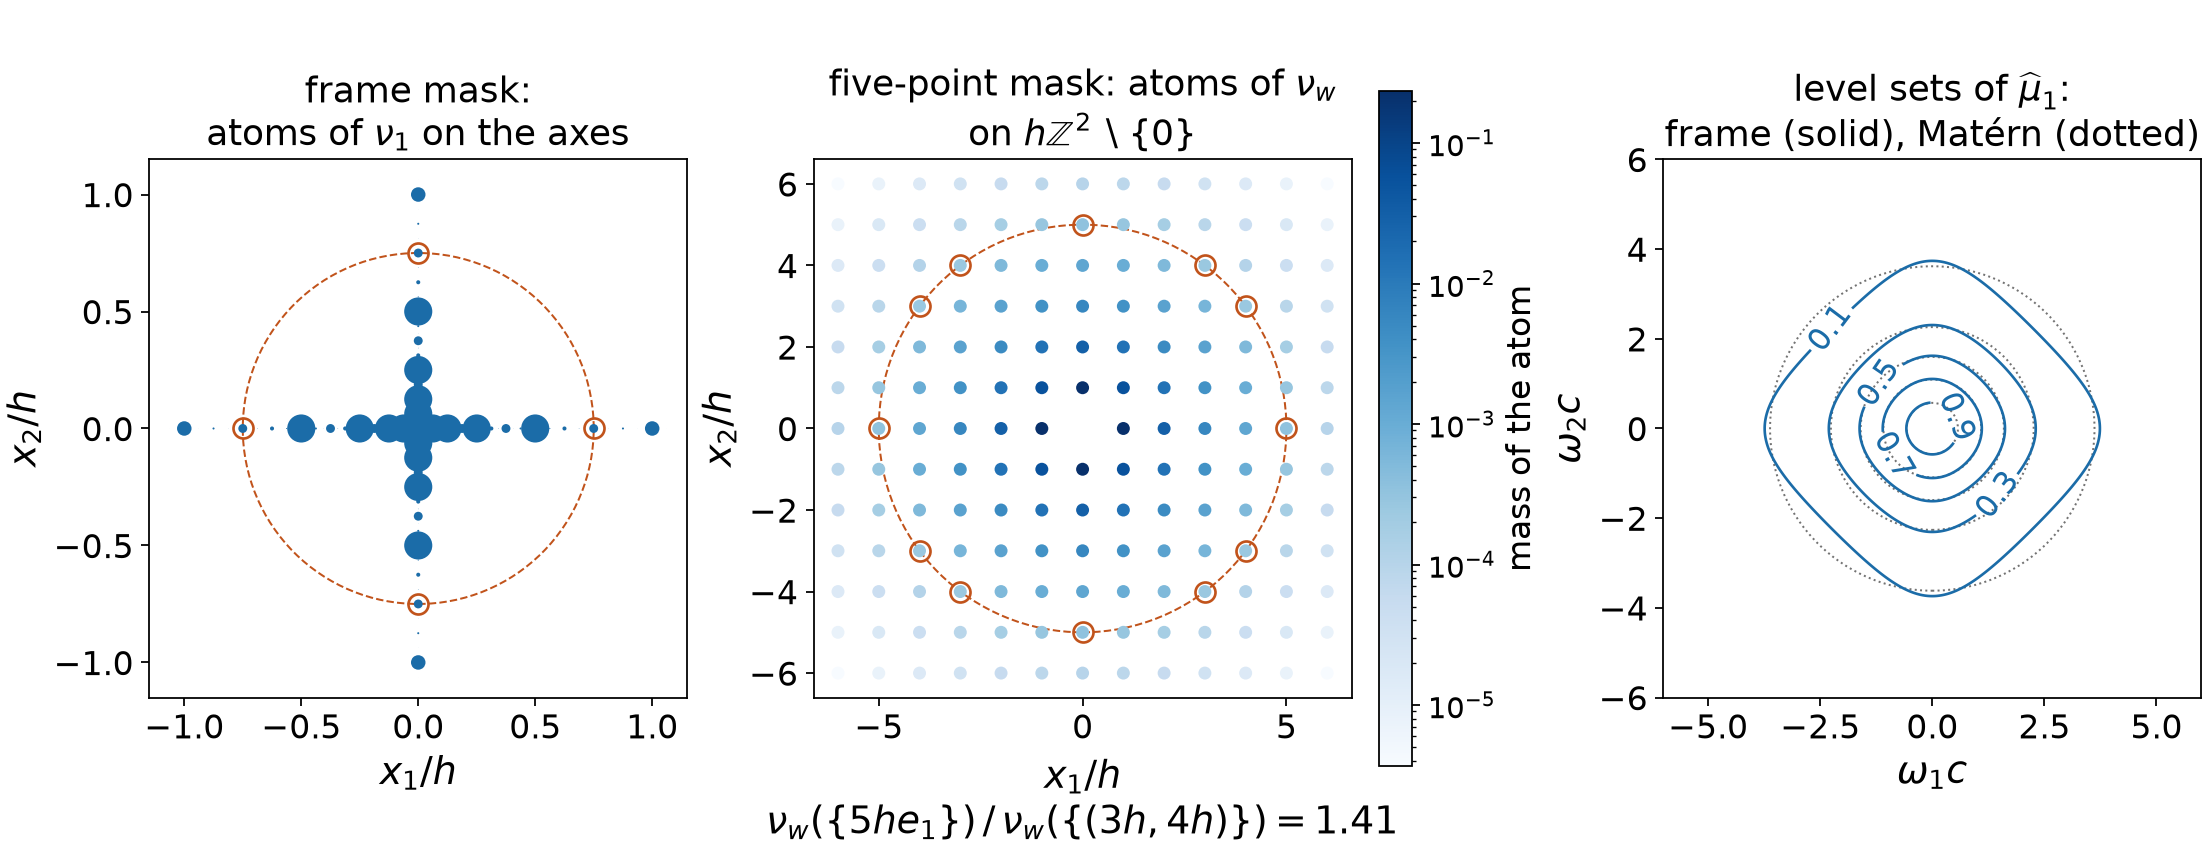
\includegraphics[width=\textwidth]{theory-frame.png}
\caption{Proposition~\ref{prop:grid-pyramid-not-isotropic}(3) on $h\ZZ^2$ with $q = 2$ and the
mask $(\lambda^{\mathrm L}_a)^{\otimes 2}$, $a = e^{-h/c}$ and $h/c = 1/2$: the sampled octave step
of the frame \Matern{} pyramid of range $c$. Left: the atoms of the \Levy{} measure $\nu_1$ of
(\ref{eq:frame-levy}) in the square $|x_i| \le 1.1h$, each of area proportional to its mass summed
over the terms $m \le 7$. The dashed circle of radius $3h/4$ meets the carrier of $\nu_1$ in its
four axis points. Middle, for comparison: the atoms of the \Levy{} measure $\nu_w$ of the five-point
resolvent mask $\kappa_t$ at $t = h$, so $p = 4/5$ in
Proposition~\ref{prop:resolvent-masks-exact}(4) and Proposition~\ref{prop:discrete-helmholtz}, on
$|x_i| \le 6h$, coloured by mass on a logarithmic scale. The series of
Proposition~\ref{prop:resolvent-masks-exact}(1) is summed over $k \le 143$, where $p^k/k$ falls
below $10^{-16}$, with each walk law computed without truncation, in double precision. Every lattice point but the origin is an atom. Of the points on the dashed circle
of radius $5h$, the twelve lattice points are atoms, with two different masses, in the ratio
$1.41$, and no other point is. Right: the level sets $0.1, 0.3, 0.5, 0.7, 0.9$ of $\widehat{\mu_1}$ (solid), against $\omega c$.
The dotted circles are the same level sets of $\exp(-F_q(|\omega|))$, the transform of the knot
kernel of the \Matern{} pyramid of Theorem~\ref{thm:matern-pyramid} with the same $q$ and $c$.
Along the diagonals the solid level sets $0.1$ to $0.7$ lie inside the circles. Both products
are cut at $m \le 59$. The solid level sets are traced by marching squares on a $601 \times 601$
mesh of $[-6, 6]^2$ in $\omega c$, and the dotted radii are read from $4000$ points of the radial
transform.}
\label{fig:theory-frame}
\end{figure}

The proof of clauses (1) and (2) reads of the dilation only that it is linear and invertible. So it
carries over to a dilation that also rotates the lattice, as in the quincunx filter banks
\cite[(2), p.~534]{kovacevic1992nonseparable} and the hexagonal pyramid
\cite[pp.~97, 99]{watson1989hexagonal}. The quincunx dilation $(x_1, x_2) \mapsto
(x_1 + x_2, x_1 - x_2)$ on $h\ZZ^2$ is $\sqrt2$ times a reflection. The proposition below assumes
neither that the dilation maps the lattice into itself nor that it is a multiple of an orthogonal
matrix, whose factor need not be the ratio $q$ of the scales.

% shared with blueprint prop:expanding-grid-pyramid-not-isotropic
\begin{proposition}[no exact grid pyramid with a matrix dilation is isotropic in $d \ge 2$]
\label{prop:expanding-grid-pyramid-not-isotropic}

Let $d \ge 2$, let $\Gamma \subset \RR^d$ be a full-rank lattice, let $w$ be a symmetric
probability law on $\Gamma$ with $w \ne \delta_0$, and let $M$ be an invertible real $d \times d$
matrix. Let $q > 1$, and let a family $(\mu_{s,t})_{0 \le s \le t}$ of probability laws on
$\RR^d$ have (a), (b) and (d) of Definition~\ref{def:exact-grid-pyramid} and, in place of (c),
\begin{enumerate}
\item[(c$_M$)] $\mu_{qs,qt} = M_*\mu_{s,t}$ for $0 \le s \le t$, where $M_*\mu$ is the image of
$\mu$ under $x \mapsto Mx$.
\end{enumerate}
Then no kernel $\mu_t$, $t > 0$, is rotation invariant. So no family with (a), (b), (c$_M$) and (d) makes the grid pyramid of $(w, M)$, the ladder $M^n_*w$ applied on the grids $M^n\Gamma$, isotropic in the sense of Definition~\ref{def:exact-grid-pyramid}.
\end{proposition}

\begin{proof}
Triplets are those of \ledger{A39}. They add under convolution, and the triplet of a law is unique.

\emph{The mask.} Every $\mu_{s,t}$ is infinitely divisible, by
Lemma~\ref{lem:steps-infinitely-divisible}, as in Proposition~\ref{prop:grid-pyramid-not-isotropic}(1).
The mask $w = \mu_{1,q}$ is carried by $\Gamma$, so by Lemma~\ref{lem:lattice-infinitely-divisible}
its triplet has Gaussian part $0$ and a finite \Levy{} measure $\nu_w$ carried by
$\Gamma \setminus \{0\}$, and $\nu_w \ne 0$ as $w \ne \delta_0$. A nonzero measure carried by a
countable set charges one of its points, so $\nu_w$ has an atom $b \ne 0$.

\emph{The steps.} By (c$_M$) at $(s/q, t/q)$, $\mu_{s,t} = M_*\mu_{s/q,t/q}$, and as $M$ is
invertible, $\mu_{s/q,t/q} = M^{-1}_*\mu_{s,t}$. By induction,
$\mu_{q^ks,q^kt} = M^k_*\mu_{s,t}$ for every integer $k$, and with (d),
$\mu_{q^{n-1},q^n} = M^{n-1}_*w$ for every integer $n$.

\emph{An atom of $\nu_t$.} Let $t > 0$, and choose an integer $n$ with $q^n \le t$. By (a),
\[
\mu_t = \mu_{q^{n-1}} * \mu_{q^{n-1},q^n} * \mu_{q^n,t} ,
\]
three infinitely divisible laws, so the \Levy{} measure $\nu_t$ of $\mu_t$ is the sum of theirs. By
\ledger{A42} with $U = M^{n-1}$, the \Levy{} measure of $\mu_{q^{n-1},q^n} = M^{n-1}_*w$ is
$M^{n-1}_*\nu_w$, as $M^{n-1}$ maps only $0$ to $0$. So $\nu_t \ge M^{n-1}_*\nu_w$, and the point
$x := M^{n-1}b \ne 0$ has $\nu_t(\{x\}) \ge \nu_w(\{b\}) > 0$.

\emph{No isotropy.} Suppose $\mu_t$ is invariant under $\mathrm{SO}(d)$. For
$R \in \mathrm{SO}(d)$, \ledger{A42} with $U = R$ gives the \Levy{} measure $R_*\nu_t$ to
$D_R\mu_t = \mu_t$, so $R_*\nu_t = \nu_t$ by uniqueness, and $\nu_t(\{Rx\}) = \nu_t(\{x\})$. As
$d \ge 2$, every point $y$ of the sphere $\{|y| = |x|\}$ is $Rx$ for some $R \in \mathrm{SO}(d)$, and
the sphere is infinite, both as in the proof of Proposition~\ref{prop:grid-pyramid-not-isotropic}(2).
So for every $N$ the sphere holds $N$ distinct points of mass $\nu_t(\{x\}) > 0$ each, and
$\nu_t(\{|y| \ge |x|\}) \ge N\nu_t(\{x\})$. But a \Levy{} measure is finite off every
neighbourhood of $0$, and $|x| > 0$. This contradiction proves the first sentence; the second is the
first, read through the definition of isotropy.

The cited facts are
\ledger{A41}, \ledger{A39} and \ledger{A42}, with \ledger{A48} through
Lemma~\ref{lem:lattice-infinitely-divisible}.
\end{proof}

\emph{On the line.} In $d = 1$ the exact grid pyramids are those that are exact in the sense of
Definition~\ref{def:grid-pyramid-line}, a definition on operators
(Proposition~\ref{prop:line-and-arrays}(1)). There Proposition~\ref{prop:grid-pyramid-not-isotropic}(2)
is empty, since $\Orth(1) = \{\pm 1\}$, and clause (1) is the product formula of
Proposition~\ref{prop:grid-pyramids-infinitely-divisible}(2) on $\Gamma = h\ZZ$.

For an integer ratio the kernels of an exact grid pyramid have no density at all, in every
dimension. The mask is carried by the grid, so its transform is $1$ on the dual grid. The knot
relation then keeps the transform of the knot kernel equal to one value along a sequence of
frequencies that tends to infinity. Clause (3) of the next proposition strengthens this to
singularity.

% shared with blueprint prop:grid-pyramid-singular-kernels
\begin{proposition}[the kernels of an exact grid pyramid are singular]
\label{prop:grid-pyramid-singular-kernels}

Let $q \ge 2$ be an integer and $h > 0$, and let $(w, q)$ be an exact grid pyramid on $h\ZZ^d$,
carried by the family $(\mu_{s,t})$.
\begin{enumerate}
\item \emph{(One value along a ray.)} For every coordinate vector $e_i$,
\[
  \widehat{\mu_1}\bigl(2\pi q^ke_i/h\bigr) = \widehat{\mu_1}\bigl(2\pi e_i/h\bigr) \ne 0,
  \qquad k \ge 0 .
\]
\item \emph{(No density.)} No kernel $\mu_t$, $t > 0$, is absolutely continuous with respect to
Lebesgue measure.
\item \emph{(Singular.)} Every kernel $\mu_t$, $t > 0$, is singular with respect to Lebesgue
measure: it is carried by a Lebesgue-null set.
\end{enumerate}
\end{proposition}

\begin{proof}
Write $\xi := 2\pi e_i/h$ and $G := h\ZZ[1/q]^d$, which is
$\bigcup_{k \ge 0}q^{-k}h\ZZ^d$ (Proposition~\ref{prop:grid-pyramid-not-isotropic}(1)).

(1) By (a), (c) and (d), $D_q\mu_1 = \mu_{0,q} = \mu_1 * w$, so
$\widehat{\mu_1}(q\omega) = \widehat{w}(\omega)\,\widehat{\mu_1}(\omega)$, as in the proof of
Lemma~\ref{lem:knot-data}. For $k \ge 0$ and $n \in \ZZ^d$,
$\langle q^k\xi, hn\rangle = 2\pi q^kn_i$ is an integer multiple of $2\pi$, $q$ being an integer.
So $e^{i\langle q^k\xi, x\rangle} = 1$ at every point $x$ of $h\ZZ^d$, which carries $w$, and
$\widehat w(q^k\xi) = 1$. Hence $\widehat{\mu_1}(q^{k+1}\xi) = \widehat{\mu_1}(q^k\xi)$, and by
induction $\widehat{\mu_1}(q^k\xi) = \widehat{\mu_1}(\xi)$ for every $k \ge 0$. The law
$\mu_1 = \mu_{0,1}$ is infinitely divisible, by Lemma~\ref{lem:steps-infinitely-divisible}, so its
transform has no zero (\ledger{A40}).

(2) Let $t > 0$, and choose an integer $n \ge 0$ with $t \le q^n$. By (a),
$\mu_{q^n} = \mu_t * \mu_{t,q^n}$, so $\widehat{\mu_{q^n}} = \widehat{\mu_{t,q^n}}\,\widehat{\mu_t}$,
and as the transform of a probability law has modulus at most $1$,
$|\widehat{\mu_t}(\omega)| \ge |\widehat{\mu_{q^n}}(\omega)|$ for every $\omega$. By (c),
$\mu_{q^n} = D_{q^n}\mu_1$, so at $\omega_k := q^k\xi$ (1) gives
$\widehat{\mu_{q^n}}(\omega_k) = \widehat{\mu_1}(q^{n+k}\xi) = \widehat{\mu_1}(\xi)$. So
$|\widehat{\mu_t}(\omega_k)| \ge |\widehat{\mu_1}(\xi)| > 0$ for every $k$, while
$|\omega_k| = 2\pi q^k/h \to \infty$. If $\mu_t$ had a density, its transform would tend to $0$ at
infinity, by the Riemann--Lebesgue lemma. So $\mu_t$ is not absolutely continuous.

(3) \emph{A random series.} Let $X_1, X_2, \dots$ be independent random vectors, $X_m$ with law
$D_{q^{-m}}w$, and $T_M := X_1 + \dots + X_M$, $T_0 := 0$, whose law is
$\rho_M := D_{q^{-1}}w * \dots * D_{q^{-M}}w$. By (\ref{eq:knot-product}), $\rho_M \to \mu_1$
weakly. A weakly convergent sequence of probability laws on $\RR^d$ is tight: for $\eta > 0$ there
is $R$ with $\rho_j(\{|x| > R\}) < \eta$ for every $j$. For $M < M'$ the difference
$T_{M'} - T_M = X_{M+1} + \dots + X_{M'}$ has the law $D_{q^{-M}}\rho_{M'-M}$, so for
$\varepsilon > 0$,
\[
  P\bigl(|T_{M'} - T_M| > \varepsilon\bigr) = \rho_{M'-M}\bigl(\{|x| > q^M\varepsilon\}\bigr) < \eta
  \qquad\text{once } q^M\varepsilon \ge R .
\]
So $(T_M)$ is a Cauchy sequence in probability. It converges in probability to a random vector
$S$, and almost surely along a subsequence, and the law of $S$ is the weak limit of the $\rho_M$,
which is $\mu_1$.

\emph{A zero-one law.} Each $X_m$ takes its values in $q^{-m}h\ZZ^d \subseteq G$. The set $G$ is a
group, the union of the increasing groups $q^{-k}h\ZZ^d$ (increasing as $q$ is an integer), so
$T_M \in G$ for every $M$. Let $A \subseteq \RR^d$ be a Borel set with $A + g = A$ for every
$g \in G$, and $E := \{S \in A\}$. Then $E = \{S - T_M \in A\}$ for every $M$. The vector
$S - T_M$ is the limit in probability of $T_{M'} - T_M$ as $M' \to \infty$, so it agrees almost
surely with the limit along a subsequence, a function of $X_{M+1}, X_{M+2}, \dots$. So $E$ agrees
almost surely with an event $E_M$ of $\mathcal{F}_M := \sigma(X_{M+1}, X_{M+2}, \dots)$, for every
$M \ge 0$. The event $E_M$ is independent of $\sigma(X_1, \dots, X_M)$, and so is $E$, which
differs from it by a null set. The union of the $\sigma(X_1, \dots, X_M)$, $M \ge 1$, is a
$\pi$-system that generates $\mathcal{F}_0$, so by the $\pi$--$\lambda$ theorem $E$ is independent
of $\mathcal{F}_0$, which contains $E_0$. Then $P(E) = P(E \cap E_0) = P(E)\,P(E_0) = P(E)^2$, and
$\mu_1(A) = P(E)$ is $0$ or $1$. This is Kolmogorov's zero-one argument as Jessen and Wintner use
it for their law of pure types [\sscite{jessen1935distribution}, Thm.~35, p.~86],
[\sscite{sato1999levy}, Prop.~27.18, p.~182].

\emph{The knot kernel is singular.} By (2), $\mu_1$ is not absolutely continuous, so some Borel set
$N$ of Lebesgue measure $0$ has $\mu_1(N) > 0$. The set $A := N + G = \bigcup_{g \in G}(N + g)$ is a
countable union of null Borel sets, so it is a null Borel set, and $A + g = A$ for $g \in G$. As
$\mu_1(A) \ge \mu_1(N) > 0$, the zero-one law gives $\mu_1(A) = 1$: $\mu_1$ is carried by the null
set $A$.

\emph{Every kernel.} Let $t > 0$, and choose $n \in \ZZ$ with $q^n \le t < q^{n+1}$. By (a),
$\mu_t = \mu_{q^n} * \mu_{q^n,t}$, and $\mu_{q^n} = D_{q^n}\mu_1$ is carried by the null set
$q^nA$. The step $\mu_{q^n,t}$ is carried by a countable set. Indeed, by (a), (c) and (d),
$D_{q^n}w = \mu_{q^n,q^{n+1}} = \mu_{q^n,t} * \mu_{t,q^{n+1}}$, three infinitely divisible laws
(Lemma~\ref{lem:steps-infinitely-divisible}), whose triplets of \ledger{A39} add. By
Proposition~\ref{prop:grid-pyramid-not-isotropic}(1) the mask has the data $(0, \nu_w)$ with
$\nu_w$ finite and carried by $h\ZZ^d \setminus \{0\}$, so the symmetric law $D_{q^n}w$ has the
triplet $(0, D_{q^n}\nu_w, 0)$. Two positive semidefinite Gaussian parts with sum $0$ vanish, so
$\mu_{q^n,t}$ has a triplet $(0, \nu', \gamma')$ with $\nu' \le D_{q^n}\nu_w$, a finite measure
carried by $q^nh\ZZ^d$. Its transform is therefore
$\exp\bigl(i\langle b, \omega\rangle + \int(e^{i\langle\omega, x\rangle} - 1)\,\nu'(dx)\bigr)$ with
$b := \gamma' - \int_{\{|x| \le 1\}}x\,\nu'(dx)$, the transform of
$\delta_b * e^{-\nu'(\RR^d)}\sum_{k \ge 0}\nu'^{*k}/k!$. So $\mu_{q^n,t}$ is this law, carried by
the countable set $C := b + q^nh\ZZ^d$. The set $q^nA + C$ is a countable union of translates of
$q^nA$, so it is null, and
\[
  \mu_t(q^nA + C) = \int\mu_{q^n}(q^nA + C - y)\,\mu_{q^n,t}(dy) = 1,
\]
since $q^nA + C - y \supseteq q^nA$ for $y \in C$. So $\mu_t$ is singular.

Clauses (1) and (2) are machine-checked, and their cited facts are \ledger{A40} and \ledger{A41};
clause (3) is proved here in print only, with \ledger{A39} and the entries of
Proposition~\ref{prop:grid-pyramid-not-isotropic}(1).
\end{proof}

The proof of (1) and (2) reads of the grid only a point $\xi \ne 0$ of its dual, with
$\langle\xi, \gamma\rangle \in 2\pi\ZZ$ for every $\gamma$ of the lattice. Every full-rank lattice
has one, so (1) and (2) hold on every full-rank lattice, with $\xi$ in place of $2\pi e_i/h$. The
pyramid principle, which reads continuous densities, therefore never applies to a family that
carries an exact grid pyramid of integer ratio.

The frame pyramid on the grid is exact, and by clause (2) it is not isotropic in $d \ge 2$.
Section~\ref{ch:matern} tests a pyramid in a second way, by the implicit-Euler principle of
Definition~\ref{def:implicit-euler-principle}. At a local maximum of the output, the output does
not exceed the input, and at a local minimum it is not below it. On the continuum this test rejects
the octave step of the frame pyramid, while each of its axis passes has the principle
(Theorem~\ref{thm:selection-stratum-two}(4)). On the grid a local maximum is read on a finite
symmetric neighbourhood $\mathcal{N}$ of lattice points. The next proposition shows that the grid
gives the same verdict, in every dimension $d \ge 2$.

% shared with blueprint prop:grid-frame-step-not-selected
\begin{proposition}[the frame step on the grid is not selected]
\label{prop:grid-frame-step-not-selected}

Let $d \ge 2$, $h > 0$ and $0 < a < 1$, and let $w := (\lambda^{\mathrm L}_a)^{\otimes d}$ be the
frame mask on $h\ZZ^d$ of Proposition~\ref{prop:grid-pyramid-not-isotropic}(3), the octave step of
the frame \Matern{} pyramid on the grid. Let $\mathcal{N}$ range over the finite symmetric sets of
nonzero points of $h\ZZ^d$, and read the principle on $\mathcal{N}$ as in
Definition~\ref{def:implicit-euler-principle}.
\begin{enumerate}
\item For every such $\mathcal{N}$, the frame mask $w$ does not have the principle on $\mathcal{N}$.
\item For each $i$, the axis pass along $e_i$, the law $\lambda^{\mathrm L}_a$ carried by the axis
$h\ZZ e_i$, has the principle on $\mathcal{N}$ for every such $\mathcal{N}$ that contains $\pm he_i$.
\end{enumerate}
\end{proposition}

\begin{proof}
We read kernels on $h\ZZ^d$ in their indices $n \in \ZZ^d$, so that $he_i$ is the index $e_i$ and
$h$ plays no further role; $\lambda := \lambda^{\mathrm L}_a$ is a kernel on $\ZZ$. Put
$\varsigma := a/(1-a)^2 > 0$.

\emph{The inverse on the line.} The values of $\lambda$ satisfy the three-point recursion
\[
(1 + 2\varsigma)\lambda(m) - \varsigma\bigl(\lambda(m+1) + \lambda(m-1)\bigr) = \delta_0(m),
\qquad m \in \ZZ .
\]
Indeed, let $c := \tfrac{1-a}{1+a}$, and note $\varsigma(1-a)^2 = a$. For $m \ne 0$ the left side
is $c\,a^{|m|-1}\bigl((1 + 2\varsigma)a - \varsigma(1 + a^2)\bigr) = c\,a^{|m|-1}\bigl(a -
\varsigma(1-a)^2\bigr) = 0$. For $m = 0$ it is $c\,(1 + 2\varsigma(1-a)) = c\,(1 + 2a/(1-a)) = 1$.
So the kernel $m_1 := (1 + 2\varsigma)\delta_0 - \varsigma(\delta_1 + \delta_{-1})$, carried by
$\{-1, 0, 1\}$, has $m_1 * \lambda = \delta_0$.

\emph{The inverse of the frame mask.} Let $M := m_1^{\otimes d}$, $M(n) := \prod_jm_1(n_j)$, a
kernel carried by the box $B := \{-1, 0, 1\}^d$. For a kernel $g$ on $\ZZ$ and $n \in \ZZ^d$, the
convolution $(M * g^{\otimes d})(n)$ is a finite sum over $B$, and expanding a product of $d$ finite
sums gives
\[
(M * g^{\otimes d})(n) = \sum_{y \in B}\prod_jm_1(y_j)\,g(n_j - y_j)
= \prod_j\,\sum_{y_j \in \{-1, 0, 1\}}m_1(y_j)\,g(n_j - y_j) .
\]
At $g = \lambda$ each factor is $\delta_0(n_j)$ by the recursion, so $M * w = \delta_0$. The mask
$w$ is summable: a finite set of indices lies in the box of its coordinates, over which the sum of
$w$ is a product of $d$ finite sums of $\lambda$, each at most $1$. Convolution of two summable
kernels is associative against a bounded function, since the double sum converges absolutely,
by the product of the two masses and the bound.

(1) Let $u := -1$ on the set $D$ of the four indices $\pm e_1 \pm e_2$ and $u := 0$ elsewhere, and
let $f := M * u$, bounded since $M$ is finitely supported and $u$ is bounded. Then
$w * f = (w * M) * u = u$, as $w * M = M * w = \delta_0$, convolution of summable kernels being
commutative. Since $u \le 0 = u(0)$, the origin is a maximum of $u$ over the whole
grid, so it is an $\mathcal{N}$-maximum for every $\mathcal{N}$. Next,
$f(0) = \sum_yM(y)\,u(-y)$. A term is nonzero only if $-y \in D$, that is $y \in D$, and there
$y_1, y_2 \in \{\pm1\}$ and $y_j = 0$ for $j \ge 3$, so
\[
M(y) = m_1(\pm1)\,m_1(\pm1)\prod_{j \ge 3}m_1(0) = \varsigma^2(1 + 2\varsigma)^{d-2} > 0 .
\]
So every term of $f(0)$ is $\le 0$, the four nonzero ones are $-\varsigma^2(1 + 2\varsigma)^{d-2}$,
and
\[
f(0) = -4\varsigma^2(1 + 2\varsigma)^{d-2} < 0 = u(0) .
\]
The principle would require $u(0) \le f(0)$ at an $\mathcal{N}$-maximum, so it fails. At $d = 2$,
$f(0) = -4\varsigma^2$.

(2) Let $\kappa$ be the law $\lambda$ carried by the axis $\ZZ e_i$, and
$m^{(i)} := (1 + 2\varsigma)\delta_0 - \varsigma(\delta_{e_i} + \delta_{-e_i})$. Then
$(m^{(i)} * \kappa)(n) = (1 + 2\varsigma)\kappa(n) - \varsigma\bigl(\kappa(n + e_i) +
\kappa(n - e_i)\bigr)$. If $n$ lies on the axis, so do $n \pm e_i$, and this is the recursion at
$n_i$, equal to $\delta_0(n_i) = \delta_0(n)$. Otherwise $n$ has a nonzero coordinate $n_j$,
$j \ne i$, which $n \pm e_i$ share, so the three values of $\kappa$ vanish, and so does
$\delta_0(n)$. So $m^{(i)} * \kappa = \delta_0$, and $\kappa$ is summable, its values being those
of $\lambda$. For a bounded $f$ and $u := \kappa * f$, associativity gives
$f = (m^{(i)} * \kappa) * f = m^{(i)} * u$, that is
\[
f(x) = u(x) + \varsigma\bigl(2u(x) - u(x + e_i) - u(x - e_i)\bigr) .
\]
At an $\mathcal{N}$-maximum $x$ of $u$ with $\pm e_i \in \mathcal{N}$ the bracket is nonnegative,
so $u(x) \le f(x)$. At an $\mathcal{N}$-minimum it is nonpositive, so $f(x) \le u(x)$.

Every step is machine-checked, with no cited fact.
\end{proof}

The proof reads the failure off the inverse of the mask. The inverse of an axis pass has
nonpositive weights off the origin. The inverse $M$ of the frame mask is the tensor power of those,
and it charges the diagonal neighbours $\pm he_1 \pm he_2$ with the positive weight
$\varsigma^2(1 + 2\varsigma)^{d-2}$. In the counterexample the origin is a maximum over the whole
grid, so the failure does not depend on the neighbourhood.

The signs of the inverse are what the principle reads, as follows. With $u := w * f$ and
$M * w = \delta_0$, the input is $f = M * u$. The weights of $M$ sum to $1$, so
$f(x) - u(x) = \sum_{y \ne 0}M(y)\bigl(u(x - y) - u(x)\bigr)$. At an $\mathcal{N}$-maximum $x$ of
$u$, every bracket with $y \in \mathcal{N}$ is at most $0$. So an inverse with nonpositive weights
off the origin, carried by $\mathcal{N} \cup \{0\}$, gives $u(x) \le f(x)$. A positive weight off
the origin can break it.

\subsection{Which masks are exact, and what the algorithm computes}
\label{sec:price-masks}

Section~\ref{sec:price-obstruction} showed what an exact pyramid on a lattice gives up. This
subsection turns to what a designer can still choose. Which masks give an exact pyramid, and what
does the pyramid algorithm compute with them? Proposition~\ref{prop:grid-pyramid-not-isotropic}(1)
gives a necessary condition: the mask is infinitely divisible. With a logarithmic moment the
condition is also sufficient, in every dimension. For laws the sufficiency is the theorem of
Maejima and Ueda [\sscite{maejima2009stochastic}, Thm.~3.3, p.~353]. Necessity follows from
continuity in scale (Lemma~\ref{lem:steps-infinitely-divisible}). The criterion does not involve
$q$, so a mask that is exact for one ratio is exact for every ratio. It can be tested on the
weights. By Proposition~\ref{prop:exact-masks}(1) an infinitely divisible mask on a lattice is
compound Poisson, so its transform is positive, and the logarithm of the transform has the absolutely
summable Fourier coefficients $\nu_w(\{x\}) \ge 0$ at the points $x \ne 0$. Conversely, a symmetric
mask whose transform is positive, with a logarithm of that kind, is the compound Poisson law of
those coefficients, and so it is infinitely divisible.
\begin{itemize}
\item Proposition~\ref{prop:exact-masks} gives the criterion. It also shows that the ladder fixes
the knot kernels but not the family between them.
\item Proposition~\ref{prop:resolvent-masks-exact} shows that the resolvent masks of a random walk
whose step has a logarithmic moment meet the criterion. A comparison with the frame mask under the
implicit-Euler principle follows it.
\item Definition~\ref{def:level-records} to Proposition~\ref{prop:binomial-records} follow an
input through the levels of the computed pyramid. In $d \ge 2$ and for an integer $q \ge 2$, one
level can create local maxima, for two exact masks and for the binomial mask.
\item Proposition~\ref{prop:line-and-arrays} says what the algorithm returns. It also shows that on
the line the two definitions of an exact grid pyramid agree.
\item Proposition~\ref{prop:binomial-knot-relation} shows why the definition requires continuity in
scale.
\end{itemize}

% shared with blueprint prop:exact-masks
\begin{proposition}[which laws have an exact ladder]
\label{prop:exact-masks}

Let $w \ne \delta_0$ be a symmetric probability law on $\RR^d$ and $q > 1$.
\begin{enumerate}
\item \emph{(Criterion.)} The following are equivalent.
\begin{enumerate}
\item[(a)] The ladder of $(w, q)$ is exact.
\item[(b)] $w$ is infinitely divisible and $\int\log_+|x|\,\nu_w(dx) < \infty$.
\item[(c)] $w$ is infinitely divisible and $\int\log_+|x|\,w(dx) < \infty$.
\end{enumerate}
If $w$ is carried by a full-rank lattice $\Gamma$, an infinitely divisible $w$ is the compound
Poisson law with a finite symmetric \Levy{} measure $\nu_w$ carried by $\Gamma \setminus \{0\}$, and
its support is unbounded.
\item \emph{(Ladder and family.)} Let $w$ be carried by a full-rank lattice $\Gamma$. If (a)--(c)
hold, the knot
kernel $\mu_1$ is that of
(\ref{eq:knot-product}), with no Gaussian part and \Levy{} measure $\nu^* := \sum_{m \ge 1}
D_{q^{-m}}\nu_w$. The families carrying the ladder are not unique. One of them is the
\emph{uniform coupling}, with \Levy{} measures $\nu_t := \nu^* + (\log_qt)\,\nu_w$ for
$t \in [1, q]$, $\nu_{q^nt} := D_{q^n}\nu_t$, and no Gaussian part.
\end{enumerate}
\end{proposition}

\begin{proof}
\emph{Data.} A symmetric infinitely divisible law has unique \Levy{} data $(A, \nu)$, so a unique
\Levy{} measure, and the triplet $(2A, \nu, 0)$, by Lemma~\ref{lem:symmetric-levy-khintchine}.
Data add under convolution, the exponents adding, and $D_c\mu$ has the data $(c^2A, D_c\nu)$ by the
substitution $y = cx$.

(1) \emph{The last sentence.} Let $w$ be carried by $\Gamma$ and infinitely divisible, with data
$(A_w, \nu_w)$. By
Lemma~\ref{lem:lattice-infinitely-divisible}, $A_w = 0$ and $\nu_w$ is finite and carried by
$\Gamma \setminus \{0\}$. So $\widehat w = e^{-\psi_w}$ with $\psi_w(\omega) := \int(1 -
\cos\langle\omega, x\rangle)\,\nu_w(dx)$, the transform of the compound Poisson law
$e^{-\nu_w(\RR^d)}\sum_{k \ge 0}\nu_w^{*k}/k!$ of the symmetric measure $\nu_w$, and by the uniqueness
of the transform $w$ is that law. It is not a point mass, a symmetric $\delta_x$ being $\delta_0$.
By Proposition~\ref{prop:no-bounded-step}, a law of bounded support that is not a point mass is not
infinitely divisible, so the support of $w$ is unbounded: $w(\{|x| > R\}) > 0$ for every $R$.

\emph{(a) implies (b).} Let $(\mu_{s,t})$ carry the ladder. Every $\mu_{s,t}$ is infinitely
divisible, by Lemma~\ref{lem:steps-infinitely-divisible}, which applies since $d \ge 1$, $w$ being
a law other than $\delta_0$. Its (I1) is condition (a) of Definition~\ref{def:exact-grid-pyramid},
convolution being commutative, and its (I2) follows from the weak continuity (b) there, as
$x \mapsto e^{i\langle\omega, x\rangle}$ is bounded and continuous. So $w = \mu_{1,q}$ is
infinitely divisible, and it has data $(A_w, \nu_w)$. By Lemma~\ref{lem:knot-data}, $\mu_1$ has the
data $(A_w/(q^2 - 1), \nu^*)$, with $\nu^* := \sum_{m \ge 1}D_{q^{-m}}\nu_w$. So $\nu^*$ is a
\Levy{} measure, and by Tonelli
\[
\int\min\bigl(1, |x|^2\bigr)\,\nu^*(dx) = \int\Bigl[\sum_{m \ge 1}\min\bigl(1,
q^{-2m}|v|^2\bigr)\Bigr]\,\nu_w(dv) < \infty .
\]
For $|v| > 1$ the $\lfloor\log_q|v|\rfloor$ terms of the bracket with $q^m \le |v|$ equal $1$, so
the bracket is at least $\log_q|v| - 1$. Hence
$\log_+|v| \le \log q\,\bigl(\text{bracket} + \mathbf 1_{\{|v| > 1\}}\bigr)$ for every $v$, and
$\nu_w(\{|v| > 1\}) < \infty$ gives $\int\log_+|x|\,\nu_w(dx) < \infty$. This is
Proposition~\ref{prop:ladder-knot-kernel}(1)'s last sentence, for a family assumed only to carry
the ladder.

\emph{(b) implies (a).} The mask $w$ is a symmetric infinitely divisible law other than $\delta_0$
with $\int\log_+|x|\,\nu_w(dx) < \infty$. By Proposition~\ref{prop:ladder-knot-kernel}(2) some
symmetric $q$-covariant family with $S_qt = qt$ has $\mu_{1,q} = w$. Its cascade (I1) is (a) of
Definition~\ref{def:exact-grid-pyramid}, convolution being commutative; the continuity (I2) of its
transforms gives the weak continuity (b) by \Levy's continuity theorem; its covariance at $q$ with
$S_qt = qt$ is (c); and $\mu_{1,q} = w$ is (d). So the ladder is exact.

\emph{(b) is equivalent to (c).} This is the equivalence of the two logarithmic moments in
Proposition~\ref{prop:ladder-knot-kernel}(2), whose proof reads \ledger{A49} with
$g(x) = \log(|x| \vee e)$.

(2) Let the conditions hold, and let $(A_w, \nu_w)$ be the data of $w$, so that $A_w = 0$ by (1).
Let $(\mu_{s,t})$ carry the ladder. As $w$ is carried by $\Gamma$, the ladder is an exact grid
pyramid on the lattice $\Gamma$, so
by Proposition~\ref{prop:grid-pyramid-not-isotropic}(1) the knot kernel is (\ref{eq:knot-product}),
with no Gaussian part and the \Levy{} measure $\nu_{q^0} = \sum_{m \ge 1}D_{q^{-m}}\nu_w = \nu^*$.

Families carrying the ladder are built by Lemma~\ref{lem:synthesis} from data on one octave. For a
weight $\ell$, continuous and strictly increasing on $[1, q]$ with $\ell(1) = 0$ and $\ell(q) = 1$,
take the data $(0, \nu_u)$, $\nu_u := \nu^* + \ell(u)\,\nu_w$, $u \in [1, q]$. Their exponents
$\Psi^*(\xi) + \ell(u)\psi_w(\xi)$, with $\Psi^*$ the exponent of $(0, \nu^*)$, are continuous in $u$;
they increase strictly, as $\psi_w \not\equiv 0$ for $w \ne \delta_0$; and they glue, as
$D_q\nu^* = \nu_w + \nu^*$. The lemma extends them to every $t = q^nu$, $u \in [1, q)$, by
$\nu_t := D_{q^n}\nu_u$, and gives laws $\mu_{s,t}$ with the transforms $e^{-(\Psi_t - \Psi_s)}$,
$\Psi_t$ the exponent of $(0, \nu_t)$ and $\Psi_0 = 0$. They form a symmetric $q$-covariant family
with $S_qt = qt$, and $\mu_{1,q}$ has the transform $e^{-(\Psi_q - \Psi_1)} = e^{-\psi_w}$, so it is
$w$, and the family meets (a)--(d) as in (b) implies (a): it carries the ladder.

\emph{Not unique.} The weights $\log_qu$ and $(\log_qu)^2$ give two such families. At
$t = q^{1/2}$ their laws $\mu_{1,t}$ have the exponents $\tfrac12\psi_w$ and $\tfrac14\psi_w$, which
differ where $\psi_w \ne 0$.

\emph{The uniform coupling} is the family of the weight $\log_q$. Its kernel $\mu_t = \mu_{0,t}$,
$t > 0$, has the transform $e^{-\Psi_t}$, so it has the data $(0, \nu_t)$: at $t = q^nu$ with
$n = \lfloor\log_qt\rfloor$ and $u = q^{-n}t \in [1, q)$, the \Levy{} measure
$D_{q^n}\bigl(\nu^* + (\log_qu)\,\nu_w\bigr)$, the measure $\nu_t$ of the statement.

Every step is machine-checked, and the cited facts are \ledger{A41}, \ledger{A39} and those of the
statements used.
\end{proof}

\emph{On the line.} Proposition~\ref{prop:exact-masks} is
Proposition~\ref{prop:grid-pyramids-infinitely-divisible}(1)--(2), with the same logarithmic
moment.

For a pyramid as it is built, clause (1) means that an exact mask on a lattice has unbounded
support. So no finite mask is exact, and truncating an exact mask makes it inexact. Clause (2)
means that the ladder fixes the knot kernels but not the laws between the knots. Two families can
carry the same ladder and differ inside an octave.

An exact mask must then be applied without truncation. On the infinite grid the resolvents of
discrete Laplacians can be. Applied to a bounded array $f$ on $h\ZZ^d$, the $(2d+1)$-point
resolvent $\kappa_t$ gives $v := \kappa_t * f$, a bounded solution of $(1 - t^2\Delta_h)v = f$,
with no truncation of $\kappa_t$. It is the only bounded one: the difference of two, added to
$\kappa_t$, would be a second bounded solution of $(1 - t^2\Delta_h)\kappa = \delta_0$
(Proposition~\ref{prop:discrete-helmholtz}(1)). Finite arrays,
with their boundaries, are left to the further work named in Section~\ref{sec:discrete-helmholtz}.
The next proposition shows that these masks are exact. Each is the law of a lattice random walk stopped at an independent
geometric time, and its \Levy{} measure is a series in the convolution powers of the step.

% shared with blueprint prop:resolvent-masks-exact
\begin{proposition}[the resolvent masks are exact]
\label{prop:resolvent-masks-exact}

Let $\sigma \ne \delta_0$ be a symmetric probability law on $\Gamma$, let $0 < p < 1$, and let
\begin{equation}\label{eq:resolvent-mask}
w := (1 - p)\sum_{k \ge 0}p^k\sigma^{*k}, \qquad \widehat{w} = \frac{1 - p}{1 - p\,\widehat{\sigma}} .
\end{equation}
\begin{enumerate}
\item $w$ is infinitely divisible. It is the compound Poisson law whose \Levy{} measure $\nu_w$ is
the restriction of $\sum_{k \ge 1}\tfrac{p^k}{k}\sigma^{*k}$ to $\Gamma \setminus \{0\}$, of total
mass at most $\log\frac{1}{1-p}$.
\item Let $\int\log_+|x|\,\sigma(dx) < \infty$, as when $\sigma$ has finite support. For every
$q > 1$ and every integer $\gamma \ge 1$ the grid pyramid of $(w^{*\gamma}, q)$ is exact, with the
knot kernel
$\widehat{\mu_1} = \prod_{m \ge 1}\widehat{w}(q^{-m}\,\cdot)^\gamma$.
\item If $d \ge 2$ and $\operatorname{supp}\sigma$ spans $\RR^d$, then for every $q > 1$ and every
integer $\gamma \ge 1$ no kernel $\mu_t$, $t > 0$, of a family carrying the ladder of
$(w^{*\gamma}, q)$ is rotation invariant. At every knot the symmetry group of the kernel is
finite, and it contains every $R \in \Orth(d)$ with $R_*\sigma = \sigma$.
\item \emph{(Instances.)} Let $\Gamma = h\ZZ^d$, and let $t > 0$, in this clause the range of a
resolvent, not a scale of the pyramid. The $(2d+1)$-point resolvent $\kappa_t$ of
Proposition~\ref{prop:discrete-helmholtz} is (\ref{eq:resolvent-mask}) with $\sigma$ the simple
random walk step and $p = 2dt^2/(h^2 + 2dt^2)$, and then $\nu_w$ charges every nonzero point
of $h\ZZ^d$. On $h\ZZ^2$ the nine-point resolvent $\kappa^9_t$ of
Proposition~\ref{prop:nine-point-family} is (\ref{eq:resolvent-mask}) with its step $\sigma_9$ and
$p = 10t^2/(3h^2 + 10t^2)$. More generally, a mask with
$1/\widehat{w}(\omega) = 1 + \sum_{y \in \mathcal{N}}c_y\bigl(1 - \cos\langle\omega, y\rangle\bigr)$,
for a finite symmetric $\mathcal{N} \subset \Gamma \setminus \{0\}$ and $c_y = c_{-y} \ge 0$ not
all $0$, is (\ref{eq:resolvent-mask}) with $C := \sum_yc_y$, $p := C/(1 + C)$ and
$\sigma := (2C)^{-1}\sum_yc_y(\delta_y + \delta_{-y})$.
\end{enumerate}
\end{proposition}

\begin{proof}
Write $\widehat{\mu}$ for the transform of a law $\mu$, $\psi_D(\omega) := \langle\omega,
A\omega\rangle + \int(1 - \cos\langle\omega, x\rangle)\,\nu(dx)$ for symmetric data $D = (A, \nu)$,
and say that $\mu$ has the data $D$ when $\widehat{\mu} = e^{-\psi_D}$.

(1) Each $\sigma^{*k}$ is a probability law, and $\sum_k(1-p)p^k = 1$, so $w$ is a probability law.
Its transform is the series of the transforms of the terms, $\widehat{\sigma^{*k}} =
\widehat{\sigma}^k$, and $|p\,\widehat{\sigma}| \le p < 1$, so
$\widehat{w} = (1-p)\sum_k(p\,\widehat{\sigma})^k = (1-p)/(1 - p\,\widehat{\sigma})$.

The law $\sigma$ is symmetric, so $\widehat{\sigma}(\omega) = z$ is real, with $|z| \le 1$, and so
is $\widehat{\sigma^{*k}}(\omega) = z^k$; as each $\sigma^{*k}$ is symmetric,
$\int(1 - \cos\langle\omega, x\rangle)\,\sigma^{*k}(dx) = 1 - z^k$. The measure
$\sum_{k \ge 1}\tfrac{p^k}{k}\sigma^{*k}$ has total mass $\sum_{k \ge 1}p^k/k = \log\frac{1}{1-p}$,
and so its restriction $\nu_w$ to $\RR^d \setminus \{0\}$ has mass at most $\log\frac{1}{1-p}$. As
$1 - \cos\langle\omega, \cdot\rangle$ is bounded and vanishes at the origin, its integral against
$\nu_w$ is the series of its integrals against the terms, and the real series
$\sum_{k \ge 1}x^k/k = -\log(1 - x)$ at $x = p$ and $x = pz$ give
\[
\int(1 - \cos\langle\omega, x\rangle)\,\nu_w(dx) = \sum_{k \ge 1}\frac{p^k}{k}\bigl(1 - z^k\bigr)
= \log(1 - pz) - \log(1 - p) .
\]
So $\widehat{w}(\omega) = (1-p)/(1-pz) = e^{-\psi(\omega)}$ with $\psi := \psi_{(0, \nu_w)}$. The
measure $\nu_w$ is symmetric, finite, and does not charge $0$, so $w$ has the symmetric data
$(0, \nu_w)$. The compound Poisson law $e^{-\nu_w(\RR^d)}\sum_{k \ge 0}\nu_w^{*k}/k!$ of $\nu_w$ has
the transform $\exp\int(e^{i\langle\omega, x\rangle} - 1)\,\nu_w(dx) = e^{-\psi(\omega)}$, the sine
part integrating to $0$, so it is $w$, by the uniqueness of the transform. It is infinitely
divisible, the $n$-th convolution power of the compound Poisson law of $\nu_w/n$ for every $n$. In
the formula of \ledger{A39}(i) the triplet $(0, \nu_w, 0)$ gives
$\exp\int(e^{i\langle\omega, x\rangle} - 1 - i\langle\omega, x\rangle\mathbf 1_{\{|x| \le 1\}})\,
\nu_w(dx) = e^{-\psi(\omega)}$, the compensator integrating an odd function against $\nu_w$. So by
the uniqueness of the triplet, \ledger{A39}(ii), $\nu_w$ is the \Levy{} measure of $w$. Each
$\sigma^{*k}$ is carried by $\Gamma$, closed under addition and countable, so $\nu_w$ is carried by
$\Gamma \setminus \{0\}$.

\emph{The powers.} Let $\gamma \ge 1$ be an integer. The law $w^{*\gamma}$ has the transform
$\widehat{w}^\gamma = e^{-\gamma\psi}$, so it has the data $(0, \gamma\nu_w)$. It is a mask on
$\Gamma$: a probability law, symmetric and carried by $\Gamma$ as a convolution power of such a
law, and not $\delta_0$. For the last, as $\sigma \ne \delta_0$, some $\omega$ has
$\widehat{\sigma}(\omega) = z < 1$, so $0 < (1-p)/(1-pz) < 1$ and
$\widehat{w^{*\gamma}}(\omega) = \bigl((1-p)/(1-pz)\bigr)^\gamma < 1$.

(2) By (1), $w^{*\gamma}$ is a mask with the data $(0, \gamma\nu_w)$. Let
$L := \int\log_+|x|\,\sigma(dx) < \infty$. For real $a, b \ge 0$,
$\log_+(a + b) \le \log_+(2\max(a, b)) \le \log 2 + \log_+a + \log_+b$, so
$\log_+|x + y| \le \log_+|x| + \log_+|y| + \log 2$ for $x, y \in \RR^d$. Integrating it against
$\sigma^{*(k-1)} \otimes \sigma$, whose image under $(x, y) \mapsto x + y$ is $\sigma^{*k}$, and
inducting on $k$ gives $\int\log_+|x|\,\sigma^{*k}(dx) \le k(L + \log 2)$. So
\[
\int\log_+|x|\,\nu_w(dx) \le \sum_{k \ge 1}\frac{p^k}{k}\,k(L + \log 2)
= (L + \log 2)\sum_{k \ge 1}p^k < \infty .
\]
So Proposition~\ref{prop:ladder-knot-kernel}(2), in the form that
Proposition~\ref{prop:exact-masks}(1) reads, makes the grid pyramid of $(w^{*\gamma}, q)$ exact,
with the moment of $\gamma\nu_w$. For a family carrying the ladder, the product formula
(\ref{eq:knot-product}) of Proposition~\ref{prop:grid-pyramid-not-isotropic}(1) gives
$\widehat{\mu_1}$ as the limit of the partial products of
$\widehat{w^{*\gamma}}(q^{-m}\cdot) = \widehat{w}(q^{-m}\cdot)^\gamma$.

(3) The law $w^{*\gamma}$ is a mask on $\Gamma$ by (1). For laws $\mu$, $\nu$ and points $x$, $y$,
$(\mu * \nu)\{x + y\} \ge \mu\{x\}\,\nu\{y\}$. Applied to $w^{*\gamma} = w^{*(\gamma - 1)} * w$ at
$0 + x$, with $w^{*(\gamma - 1)}\{0\} \ge w\{0\}^{\gamma - 1} \ge (1-p)^{\gamma - 1}$ and
$w\{x\} \ge (1-p)p\,\sigma\{x\}$ (the terms $k = 0$ and $k = 1$ of (\ref{eq:resolvent-mask})), it
gives $w^{*\gamma}\{x\} > 0$ at every atom $x$ of $\sigma$. So the atoms of $w^{*\gamma}$ span
$\RR^d$, and Proposition~\ref{prop:grid-pyramid-not-isotropic}(2) applies to every family carrying
the ladder: no kernel $\mu_t$, $t > 0$, is invariant under $\mathrm{SO}(d)$, and the symmetry group of every
knot kernel is finite.

Let $R \in \Orth(d)$ with $R_*\sigma = \sigma$, that is $\widehat{\sigma}(R^{\tp}\omega) =
\widehat{\sigma}(\omega)$ for every $\omega$. Then $\widehat{w^{*\gamma}}$, a function of
$\widehat{\sigma}$, is invariant in the same way, and so is every partial product of
(\ref{eq:knot-product}), since $R^{\tp}$ commutes with the dilations. The limit
$\widehat{\mu_1}$ is invariant, so $R_*\mu_1 = \mu_1$. By (c) of
Definition~\ref{def:exact-grid-pyramid} the kernel at the knot $q^n$ is $D_{q^n}\mu_1$, whose
transform is $\widehat{\mu_1}(q^n\cdot)$, invariant too.

(4) Read a kernel $\kappa$ on $\ZZ^d$ as the law $\sum_n\kappa(n)\delta_{hn}$ on $h\ZZ^d$; its
transform is the Fourier series $\sum_n\kappa(n)e^{i\langle n, \vartheta\rangle}$ at
$\vartheta = h\omega$. A probability kernel whose Fourier series is real, and with
$\kappa(0) \ne 1$, is a mask on $h\ZZ^d$: symmetric because its transform is real, and not
$\delta_0$. The simple random walk step $\sigma$ and the nine-point step $\sigma_9$ are such
kernels, with $\sigma(0) = \sigma_9(0) = 0$ and real Fourier series
(Propositions~\ref{prop:discrete-helmholtz} and~\ref{prop:nine-point-family}), carried by the
$2d$, resp.\ $8$, points of their stencils.

For a probability step $\eta$ on $\ZZ^d$ with a real Fourier series
$\varphi = \widehat{\eta}(\vartheta)$ and $a > 0$, the kernel $(1 - p)\sum_kp^k\eta^{*k}$,
$p = a/(1+a)$, has the Fourier series $(1-p)/(1 - p\varphi)$, by the geometric series as in (1),
and
\[
\frac{1 - p}{1 - p\varphi} = \frac{1/(1+a)}{(1 + a(1-\varphi))/(1+a)} = \bigl(1 + a(1 - \varphi)\bigr)^{-1} .
\]
Read on $h\ZZ^d$, it is the resolvent mask (\ref{eq:resolvent-mask}) of the law of $\eta$ with the
same $p$, the two laws having the same transform. The resolvent $\kappa_t$ of
Proposition~\ref{prop:discrete-helmholtz} is this kernel with
$\eta = \sigma$ and $a = 2dt^2/h^2$, and $\kappa^9_t$ of Proposition~\ref{prop:nine-point-family}
is this kernel with $\eta = \sigma_9$ and $a = \tfrac{10}{3}t^2/h^2$, as those propositions define
them; then $a/(1+a) = 2dt^2/(h^2 + 2dt^2)$, resp.\ $10t^2/(3h^2 + 10t^2)$.

For the simple random walk step and $n \in \ZZ^d \setminus \{0\}$, let $N := \sum_i|n_i| \ge 1$.
By induction on $N$, $\sigma^{*N}\{hn\} > 0$: if $n_i \ne 0$, let $e := \pm e_i$ with the sign of
$n_i$; then $\sum_i|(n - e)_i| = N - 1$, and $\sigma^{*N}\{hn\} \ge \sigma^{*(N-1)}\{h(n - e)\}\,
\sigma\{he\}$ with $\sigma\{he\} = 1/(2d)$. The point $hn$ is not $0$, so the term $k = N$ of
$\nu_w$ charges it, with the weight $\tfrac{p^N}{N}\sigma^{*N}\{hn\} > 0$.

For the last sentence, $C > 0$ as the $c_y$ are nonnegative and not all $0$. The law
$\sigma = (2C)^{-1}\sum_yc_y(\delta_y + \delta_{-y})$ has total mass $1$, is carried by the
symmetric $\mathcal{N} \not\ni 0$, so it is not $\delta_0$, and has the real transform
$\widehat{\sigma} = C^{-1}\sum_yc_y\cos\langle y, \cdot\rangle$, so it is symmetric. With
$S(\omega) := \sum_yc_y\cos\langle y, \omega\rangle \le C$,
\[
1 + \sum_yc_y\bigl(1 - \cos\langle\omega, y\rangle\bigr) = 1 + C - S(\omega) ,\qquad
\frac{1 - p}{1 - p\,\widehat{\sigma}(\omega)} = \frac{1/(1+C)}{(1 + C - S(\omega))/(1 + C)}
= \frac{1}{1 + C - S(\omega)} ,
\]
with $p = C/(1+C)$. So $\widehat{w} = (1 - p)/(1 - p\,\widehat{\sigma})$, and $w$ is
(\ref{eq:resolvent-mask}) by the uniqueness of the transform.

Every step is machine-checked, and the cited facts are \ledger{A39} and those of the statements
used.
\end{proof}

For an integer $q \ge 2$, a pyramid that applies the five-point or nine-point resolvent on each
grid and decimates computes the ladder of an exact grid pyramid
(Proposition~\ref{prop:line-and-arrays}(2)). By clause (3) that pyramid is not isotropic.

The resolvent masks and the frame mask are both exact, but they differ under the implicit-Euler
principle. By (\ref{eq:resolvent-mask}), $1/\widehat w = (1 - p\,\widehat\sigma)/(1 - p)$, the
transform of the signed kernel $(\delta_0 - p\sigma)/(1-p)$. This kernel is the inverse of the
resolvent mask, and its weights off the origin are nonpositive. The frame mask
$(\lambda^{\mathrm L}_a)^{\otimes d}$ is exact (Proposition~\ref{prop:grid-pyramid-not-isotropic}(3)),
but in $d \ge 2$ it is not of the form (\ref{eq:resolvent-mask}). Its inverse charges the diagonal neighbours
with a positive weight, as the proof of Proposition~\ref{prop:grid-frame-step-not-selected}
computes. The identity after that proposition shows why these signs matter for the principle. For
the $(2d+1)$-point resolvent, whose step $\sigma$ is carried by the $2d$ axis neighbours, the
principle holds on $\operatorname{supp}\sigma \setminus \{0\}$, the axis neighbours
(Proposition~\ref{prop:stage-lemma}(2)). In $d \ge 2$ the frame mask has it on no finite symmetric
neighbourhood (Proposition~\ref{prop:grid-frame-step-not-selected}(1)).

The next question is about local maxima. On the continuum in $d \ge 2$, one step of every
absolutely continuous law can create a local maximum, and the count
can rise at every rung of the \Matern{} and frame \Matern{} ladders, for an input that depends on
the rung (Proposition~\ref{prop:creation-plane}(1), (3)). So in the plane the requirement that no
octave step create a local maximum, for an arbitrary input, excludes every pyramid whose octave
steps are absolutely continuous. Can the count also grow inside a pyramid as computed, from one decimated level to the next?
In $d \ge 2$ and for an integer $q \ge 2$ it can. It does so for the $(2d+1)$-point resolvent, for
the frame mask and for the binomial mask, which is not exact
(Propositions~\ref{prop:creation-grid-masks} and~\ref{prop:binomial-records}).

The tool is the creation of local maxima on a grid, Proposition~\ref{prop:creation-grid}, which is
stated for one smoothing step. A local maximum there is read on a finite symmetric neighbourhood
$\mathcal{N}$ that contains the $2d$ axis neighbours, and this condition on $\mathcal{N}$ is kept
below. Clauses (1)--(2) need only a symmetric mask other than $\delta_0$, in $d \ge 2$. To place
that step inside a pyramid, the array that the pyramid holds after some number of levels must be
allowed to be arbitrary. Clause (3) gives this for an infinitely divisible mask. The next
definition names the arrays that the pyramid holds.

% shared with blueprint def:level-records
\begin{definition}[the records of an input]
\label{def:level-records}

Let $\Gamma \subset \RR^d$ be a full-rank lattice, $q \ge 1$ an integer, $q = 1$ being the computation without decimation, and $w$ a probability law on
$\Gamma$. The \emph{records} of a bounded function $f$ on $\Gamma$ are the arrays $f_k$ on
$q^k\Gamma$, $k \ge 0$, given by
\[
f_0 := f, \qquad f_{j+1} := \bigl(D_{q^j}w * f_j\bigr)\big|_{q^{j+1}\Gamma}, \quad j \ge 0 .
\]
The array $f_k$ is the \emph{level-$k$ record} of $f$. The convolution at a point of
$q^{j+1}\Gamma \subseteq q^j\Gamma$ reads $f_j$ only on $q^j\Gamma$, since $D_{q^j}w$ is carried by
$q^j\Gamma$, and every record is bounded by $\sup|f|$.
\end{definition}

The next lemma is the reduction that Propositions~\ref{prop:creation-grid-masks}
and~\ref{prop:binomial-records} share. On $h\ZZ^d$, if every bounded array at level $k$ is a record,
the creation of Proposition~\ref{prop:creation-grid}(1)--(2) at the spacing $q^kh$ happens inside a
pyramid.

% shared with blueprint lem:records-creation
\begin{lemma}[a mask whose records exhaust the bounded arrays creates maxima]
\label{lem:records-creation}

Let $d \ge 2$, $h > 0$, let $q \ge 2$ and $k \ge 0$ be integers, and let $w \ne \delta_0$ be a
symmetric probability law on $h\ZZ^d$. Let $\mathcal{N}$ be a
neighbourhood as in Proposition~\ref{prop:creation-grid}. Suppose that every bounded array on
$q^kh\ZZ^d$ is the level-$k$ record of a bounded input on $h\ZZ^d$. Then there is a bounded input on
$h\ZZ^d$ whose level-$k$ record has exactly one $q^k\mathcal{N}$-maximum, while the smoothing of that
record by $D_{q^k}w$ has at least two $q^k\mathcal{N}$-maxima, and the level-$(k+1)$ record has at
least two $q^{k+1}\mathcal{N}$-maxima.
\end{lemma}

\begin{proof}
The mask of the level-$k$ step, $D_{q^k}w$, is a symmetric probability law on $q^kh\ZZ^d$ other
than $\delta_0$, since $D_{q^k}$ is a bijection of $h\ZZ^d$ onto $q^kh\ZZ^d$ that commutes with
$x \mapsto -x$. The set $q^k\mathcal{N}$ is a finite symmetric subset of $q^kh\ZZ^d \setminus \{0\}$
that contains the $2d$ axis neighbours $\pm q^khe_i$, because $\mathcal{N}$ is such a subset of
$h\ZZ^d \setminus \{0\}$ and contains $\pm he_i$. So the hypotheses of
Proposition~\ref{prop:creation-grid} hold at the spacing $q^kh$, with the mask $D_{q^k}w$ and the
neighbourhood $q^k\mathcal{N}$, and its clauses (1)--(2) give a summable $f_k > 0$ on $q^kh\ZZ^d$
with exactly one $q^k\mathcal{N}$-maximum,
such that $D_{q^k}w * f_k$ has at least two $q^k\mathcal{N}$-maxima and its restriction to
$q^{k+1}h\ZZ^d$ has at least two $q^{k+1}\mathcal{N}$-maxima. Being positive and summable, $f_k$ is
bounded by its sum: $f_k(x) \le \sum_yf_k(y)$ for every $x$. By the hypothesis, $f_k$ is the
level-$k$ record of a bounded input $f$ on $h\ZZ^d$. By Definition~\ref{def:level-records}, the
level-$(k+1)$ record of $f$ is $D_{q^k}w * f_k$ restricted to $q^{k+1}h\ZZ^d$, which has the two
maxima.
\end{proof}

% shared with blueprint prop:creation-grid-masks
\begin{proposition}[the masks of the creation on a grid]
\label{prop:creation-grid-masks}

Let $d \ge 2$ and $h > 0$. Let $\beta := \tfrac{1}{16}(\delta_{-2h} + 4\delta_{-h} + 6\delta_0 +
4\delta_h + \delta_{2h})$ be the binomial mask on $h\ZZ$.
\begin{enumerate}
\item Each of the following is a symmetric probability law on $h\ZZ^d$, different from
$\delta_0$: the $(2d+1)$-point resolvent $\kappa_t$ of
Proposition~\ref{prop:discrete-helmholtz}, $t > 0$; the frame mask
$(\lambda^{\mathrm L}_a)^{\otimes d}$ of Proposition~\ref{prop:grid-pyramid-not-isotropic}(3),
$0 < a < 1$; and the tensor power $\beta^{\otimes d}$. So
Proposition~\ref{prop:creation-grid}(1)--(2) applies to each of them.
\item The first two are infinitely divisible. The third is not.
\item Let $w$ be one of the first two, $q \ge 2$ an integer, $k \ge 0$ an integer, and
$\mathcal{N}$ a neighbourhood as in Proposition~\ref{prop:creation-grid}. There is a bounded input
on $h\ZZ^d$ whose level-$k$ record (Definition~\ref{def:level-records}) has exactly one $q^k\mathcal{N}$-maximum, while the smoothing of
that record by $D_{q^k}w$ has at least two $q^k\mathcal{N}$-maxima, and the level-$(k+1)$ record
has at least two $q^{k+1}\mathcal{N}$-maxima.
\end{enumerate}
\end{proposition}

\begin{proof}
\emph{Tensor powers.} Let $c \ge 0$ be summable on $\ZZ$, $\lambda$ the law on $h\ZZ$ with the
weight $c(n)$ at $hn$, and $K(n) := \prod_ic(n_i)$ on $\ZZ^d$. The law on $h\ZZ^d$ with the
weight $K(n)$ at $hn$ is $\lambda^{\otimes d}$. Both are finite measures on $\RR^d$, and a product
measure is determined by its values on boxes $s_1 \times \dots \times s_d$. On a box the first is
$\sum_{n \in \ZZ^d}\prod_ic(n_i)\mathbf{1}[hn_i \in s_i] = \prod_i\sum_{m \in \ZZ}
c(m)\mathbf{1}[hm \in s_i]$, a finite product of sums of nonnegative terms, which is the value of
the second. When $\lambda$ is a probability, so is $\lambda^{\otimes d}$, so $\sum_nK(n) = 1$, and
the transform of $K$ is that of $\lambda^{\otimes d}$, the product $\prod_i\widehat{\lambda}(\omega_i)$.
If $c$ is symmetric, so is $K$, and $K(0) = c(0)^d$.

(1) By Proposition~\ref{prop:discrete-helmholtz}(1), $\kappa_t$, a law on $\ZZ^d$ read on $h\ZZ^d$
through $n \mapsto hn$ (so that its variable is $\vartheta = h\omega$), is a probability law with the
transform
\[
\widehat{\kappa_t}(\omega) = \Bigl(1 + \frac{t^2}{h^2}\sum_{i=1}^d(2 - 2\cos h\omega_i)\Bigr)^{-1},
\]
which that proposition writes through its frequency symbol $D_h$. It is symmetric, as a mixture of
the powers of the symmetric step $\sigma$. It is not $\delta_0$: at $h\omega = (\pi, \dots, \pi)$
its transform is $(1 + 4dt^2/h^2)^{-1} < 1$, while that of $\delta_0$ is $1$. The law
$\lambda^{\mathrm L}_a$ is symmetric and has mass $\tfrac{1-a}{1+a}(1 + \tfrac{2a}{1-a}) = 1$. By
the step on tensor powers, its tensor power is a symmetric probability, and its weight at the origin
is $(\tfrac{1-a}{1+a})^d < 1$. The mask $\beta$ is symmetric with mass $16/16 = 1$, so
$\beta^{\otimes d}$ is a symmetric probability, and its weight at the origin is $(6/16)^d < 1$.

(2) $\kappa_t$ is the mask (\ref{eq:resolvent-mask}) for the simple random walk step, by
Proposition~\ref{prop:resolvent-masks-exact}(4), so it is infinitely divisible by
Proposition~\ref{prop:resolvent-masks-exact}(1). The frame mask $w := (\lambda^{\mathrm L}_a)^{\otimes d}$, read through the step on tensor powers as
the array of products, has the transform
$\widehat{w}(\omega) = \exp\bigl(-\int(1 - \cos\langle\omega, x\rangle)\,\nu_w(dx)\bigr)$ with a
finite symmetric measure $\nu_w$ without atom at $0$, computed in the proof of
Proposition~\ref{prop:grid-pyramid-not-isotropic}(3) (``The mask in $\RR^d$''). The compound
Poisson law $e^{-\nu_w(\RR^d)}\sum_{k \ge 0}\nu_w^{*k}/k!$ has the transform
$\exp\int(e^{i\langle\omega, x\rangle} - 1)\,\nu_w(dx) = \widehat{w}(\omega)$, the sine part
integrating to $0$, so it is $w$, by the uniqueness of the transform. It is infinitely divisible,
the $n$-th convolution power of the compound Poisson law of $\nu_w/n$ for every $n$. The law
$\beta^{\otimes d}$ is carried by the ball of radius $2h\sqrt d$, each factor being carried by
$[-2h, 2h]$. It is no point mass: by
$\cos^4\theta = \tfrac18(3 + 4\cos 2\theta + \cos 4\theta)$,
\[
\widehat{\beta}(\omega) = \tfrac{1}{16}\bigl(6 + 8\cos h\omega + 2\cos 2h\omega\bigr) =
\cos^4(h\omega/2),
\]
and the transform $\prod_i\widehat{\beta}(\omega_i)$ of $\beta^{\otimes d}$ vanishes at
$\omega = (\pi/h)e_1$, where that of a point mass has modulus $1$. By
Proposition~\ref{prop:no-bounded-step} it is not infinitely divisible.

(3) By (1), $w$ is a symmetric probability law on $h\ZZ^d$ other than $\delta_0$. By (2) it is
infinitely divisible, and $q$ is an integer, so Proposition~\ref{prop:creation-grid}(3) makes every
bounded array on $q^kh\ZZ^d$ the level-$k$ record of a bounded input on $h\ZZ^d$.
Lemma~\ref{lem:records-creation} gives the input.
\end{proof}

So in $d \ge 2$, for an integer $q \ge 2$, the count of local maxima can grow under the
$(2d+1)$-point resolvent and the frame mask from one level of the pyramid to the next. This happens
at any chosen level $k$, for an input that depends on $k$, both before and after decimation. The
binomial tensor mask needs another route. It is not infinitely divisible and its transform vanishes, so
Proposition~\ref{prop:creation-grid}(3), whose proof inverts the mask, does not apply to it.
Decimation helps here. It is enough to invert the subsample of the mask on the coarse grid, and the
transform of that subsample has no zero.

% shared with blueprint prop:binomial-records
\begin{proposition}[the records of the binomial masks]
\label{prop:binomial-records}

Let $d \ge 2$, $h > 0$, let $q \ge 2$ be an integer, let $\beta$ be the binomial mask of
Proposition~\ref{prop:creation-grid-masks} and $w := \beta^{\otimes d}$ on $h\ZZ^d$.
\begin{enumerate}
\item For every integer $k \ge 0$, every bounded array on $q^kh\ZZ^d$ is the level-$k$ record
(Definition~\ref{def:level-records}) of a bounded input on $h\ZZ^d$.
\item Let $k \ge 0$ be an integer and $\mathcal{N}$ a neighbourhood as in
Proposition~\ref{prop:creation-grid}. There is a bounded input on $h\ZZ^d$ whose level-$k$ record
has exactly one $q^k\mathcal{N}$-maximum, while the smoothing of that record by $D_{q^k}w$ has at
least two $q^k\mathcal{N}$-maxima, and the level-$(k+1)$ record has at least two
$q^{k+1}\mathcal{N}$-maxima.
\end{enumerate}
\end{proposition}

\begin{proof}
(1) \emph{The subsampled mask.} Let $s$ be the kernel on $\ZZ$ that reads $\beta$ on $qh\ZZ$:
$s(m) := \beta(\{qmh\})$. The mask $\beta$ charges only $0, \pm h, \pm 2h$, so $s$ is carried by
$\{-1, 0, 1\}$: at $q = 2$ it is $s = \tfrac{1}{16}(\delta_{-1} + 6\delta_0 + \delta_1)$, and at
$q \ge 3$ it is $s = \tfrac{6}{16}\delta_0$. Its inverse on $\ZZ$ is explicit. At $q \ge 3$ put
$s^{-1} := \tfrac{16}{6}\delta_0$. At $q = 2$ let $\rho := 2\sqrt2 - 3$, the root of
$\rho^2 + 6\rho + 1 = 0$ with $|\rho| < 1$, and put $s^{-1}(n) := 2\sqrt2\,\rho^{|n|}$, summable on
$\ZZ$. Then $\sum_j s(j)s^{-1}(n - j) = \tfrac{2\sqrt2}{16}\bigl(\rho^{|n-1|} + 6\rho^{|n|} +
\rho^{|n+1|}\bigr)$, which is $\tfrac{2\sqrt2}{16}\rho^{|n|-1}(1 + 6\rho + \rho^2) = 0$ at $n \ne 0$
and $\tfrac{2\sqrt2}{16}(6 + 2\rho) = \tfrac{2\sqrt2 \cdot 4\sqrt2}{16} = 1$ at $n = 0$. So
$s * s^{-1} = \delta_0$ in both cases.

Put $S := s^{\otimes d}$ and $S^{-1} := (s^{-1})^{\otimes d}$ on $\ZZ^d$. $S$ is carried by the box
$\{-1, 0, 1\}^d$, and $S^{-1}$ is summable, $|S^{-1}|$ being the tensor power of the summable
kernel $|s^{-1}|$. So $(S * S^{-1})(n) = \sum_{m \in \{-1,0,1\}^d}\prod_i s(m_i)s^{-1}(n_i - m_i) =
\prod_i\sum_{j \in \{-1,0,1\}}s(j)s^{-1}(n_i - j) = \prod_i\delta_0(n_i)$, a finite sum of products
being the product of the sums: $S * S^{-1} = \delta_0$. Since $w(\{qhm\}) = \prod_i\beta(\{qhm_i\})
= S(m)$ for $m \in \ZZ^d$, $S$ is the subsample of $w$ on $qh\ZZ^d$.

\emph{One step.} Let $j \ge 0$ and let $g$ be a bounded array on $q^{j+1}h\ZZ^d$. Write
$G(m) := g(q^{j+1}hm)$, $m \in \ZZ^d$, and $V := S^{-1} * G$, bounded by
$\sum|S^{-1}|\cdot\sup|G|$. Then $S * V = (S * S^{-1}) * G = G$, the convolution of two summable
kernels and a bounded one being associative. Define $u$ on $q^jh\ZZ^d$ by $u(q^{j+1}hm) := V(m)$ and
$u := 0$ off $q^{j+1}h\ZZ^d$; it is bounded. The mask of step $j$, $D_{q^j}w$, has the weight
$w(\{hn\})$ at $q^jhn$, and $u$ vanishes off $q^{j+1}h\ZZ^d$, so the sum defining the smoothing at
$q^{j+1}hm$ runs over $q^{j+1}h\ZZ^d$:
\begin{align*}
(D_{q^j}w * u)(q^{j+1}hm) &= \sum_{m' \in \ZZ^d}w\bigl(\{qh(m - m')\}\bigr)\,V(m') = (S * V)(m)
= g(q^{j+1}hm).
\end{align*}
So $g$ is the array that step $j$ keeps from the bounded $u$.

\emph{All levels.} By induction on $k$. The level-$0$ record of $f$ is $f$ itself. Let $k \ge 1$
and $g$ bounded on $q^kh\ZZ^d$. The step $j = k-1$ gives a bounded $u$ on $q^{k-1}h\ZZ^d$ whose
smoothing by $D_{q^{k-1}}w$, kept on $q^kh\ZZ^d$, is $g$. By induction $u$ is the level-$(k-1)$
record of a bounded input $f$ on $h\ZZ^d$. Then $g$ is the level-$k$ record of $f$, by the
recursion of Definition~\ref{def:level-records}. The argument reads no bound on $d$.

(2) By Proposition~\ref{prop:creation-grid-masks}(1), $w$ is a symmetric probability law on
$h\ZZ^d$ other than $\delta_0$, its weight at $0$ being $(6/16)^d < 1$. By (1) every bounded array
on $q^kh\ZZ^d$ is the level-$k$ record of a bounded input, and Lemma~\ref{lem:records-creation}
gives the input.
\end{proof}

So the binomial tensor masks create local maxima as well, at any chosen level $k$ for an input
that depends on $k$, before and after decimation, for every integer $q \ge 2$
(Proposition~\ref{prop:binomial-records}(2)). Nothing is claimed on records at a non-integer $q$.
None of this conflicts with the implicit-Euler principle of
Definition~\ref{def:implicit-euler-principle}. The principle bounds the value at an
$\mathcal{N}$-maximum and says nothing about how many there are.

The records are the arrays the pyramid algorithm holds. Which law does the algorithm apply to the
input to reach them, and is it a law of the family? The next proposition answers this. It also
settles a point of definition on the line. Section~\ref{sec:line-theory} defined an exact grid
pyramid on the line through operators (Definition~\ref{def:grid-pyramid-line}), and
Definition~\ref{def:exact-grid-pyramid} uses laws. The two agree.

% shared with blueprint prop:line-and-arrays
\begin{proposition}[the line, and the arrays]
\label{prop:line-and-arrays}

\begin{enumerate}
\item \emph{(The line.)} In $d = 1$ a grid pyramid is exact in the sense of
Definition~\ref{def:exact-grid-pyramid}, on laws, if and only if it is exact in the sense of
Definition~\ref{def:grid-pyramid-line}, on operators. So the two definitions name the same
pyramids at $d = 1$, and this equivalence is what identifies them.
\item \emph{(The arrays.)} Let $q \ge 1$ be an integer ($q = 1$ is the computation without decimation), $w$ a probability law on $\Gamma$ and $f$
bounded on $\Gamma$. The algorithm that, for $k = 0, \dots, n-1$, smooths by $D_{q^k}w$ on
$q^k\Gamma$ and keeps the values on $q^{k+1}\Gamma$ returns the level-$n$ record of $f$
(Definition~\ref{def:level-records}), which is
$\bigl(D_{q^{n-1}}w * \dots * D_qw * w * f\bigr)$ restricted to $q^n\Gamma$. If $q \ge 2$ and the
grid pyramid of $(w, q)$ is exact, this is the ladder increment $\mu_{1,q^n}$ applied to $f$ and read on the coarse
grid, so the computation is exact in sense (i) for that increment, in every dimension.
\end{enumerate}
\end{proposition}

\begin{proof}
(1) In $d = 1$ a full-rank lattice is $h\ZZ$ for some $h > 0$. Definition~\ref{def:grid-pyramid-line}
requires a $q^{\ZZ}$-covariant family of operators (Definition~\ref{def:q-covariant-line}) in the
canonical discrete gauge $S_qt = qt$ of Lemma~\ref{lem:family-dilations}(3), whose kernels have the
steps $\mu_{q^n,q^{n+1}} = T_{q^n}w$. On the line $T_c = D_c$.

\emph{Exact on operators implies exact on laws.} Let $(\Phi_{s,t})$ be a family as in
Definition~\ref{def:grid-pyramid-line}, with kernels $\mu_{s,t}$. Read through its kernels
(Lemma~\ref{lem:line-axioms-kernels}(1)), it is a symmetric family of laws in dimension $1$. Its
cascade (I1) is (a) of Definition~\ref{def:exact-grid-pyramid}, convolution being commutative, and
the continuity (I2) of its transforms gives the weak continuity (b) by \Levy's continuity theorem.
Its covariance in the canonical discrete gauge is $T_q\mu_{s,t} = \mu_{qs,qt}$
(Lemma~\ref{lem:line-axioms-kernels}(3) with $\lambda = q$ and $S = S_q$), which is (c), and the
step $n = 0$ of the ladder is $\mu_{1,q} = T_1w = w$, which is (d). So the kernels carry the grid
pyramid in the sense of Definition~\ref{def:exact-grid-pyramid}.

\emph{Exact on laws implies exact on operators.} Let $(\mu_{s,t})$ carry the grid pyramid in the
sense of Definition~\ref{def:exact-grid-pyramid}. Here $\RR$ is $\RR^d$ at $d = 1$, and $w$ is a
symmetric probability law other than $\delta_0$, carried by the lattice $h\ZZ$. By the criterion
of Proposition~\ref{prop:exact-masks}(1), at $d = 1$, $w$ is infinitely divisible with
$\int\log_+|x|\,w(dx) < \infty$. That is the second criterion of
Proposition~\ref{prop:grid-pyramids-infinitely-divisible}(2), so the grid pyramid of $(w, q)$ is
exact in the sense of Definition~\ref{def:grid-pyramid-line}: a $q^{\ZZ}$-covariant family of
operators in the canonical discrete gauge has the steps of the ladder.

(2) As $q$ is an integer, $q\Gamma \subseteq \Gamma$, so the grids $q^k\Gamma$ are nested. The law
$D_{q^k}w$ is carried by $q^k\Gamma$, so for $x \in q^k\Gamma$
\[
(D_{q^k}w * g)(x) = \sum_{y \in q^k\Gamma}(D_{q^k}w)(\{y\})\,g(x - y)
\]
uses only the values of $g$ on $q^k\Gamma$: decimation discards nothing the later steps read. Let
$g_0 := f$ and let $g_{k+1}$ be $D_{q^k}w * g_k$ restricted to $q^{k+1}\Gamma$, the array the
algorithm holds after step $k$. These are the records of $f$ (Definition~\ref{def:level-records}). Put $F_k := D_{q^{k-1}}w * \dots * w * f$ on $\Gamma$, with
$F_0 := f$. If $g_k$ is $F_k$ restricted to $q^k\Gamma$, then for $x \in q^{k+1}\Gamma$ the display
gives $g_{k+1}(x) = (D_{q^k}w * F_k)(x) = F_{k+1}(x)$. By induction the algorithm returns $F_n$
restricted to $q^n\Gamma$. If the pyramid is exact, (a), (c) and (d) of
Definition~\ref{def:exact-grid-pyramid} give
\[
\mu_{1,q^n} = \mu_{q^{n-1},q^n} * \dots * \mu_{q,q^2} * \mu_{1,q} = D_{q^{n-1}}w * \dots * D_qw * w,
\]
so the returned array is $\mu_{1,q^n} * f$ restricted to $q^n\Gamma$. It equals the lattice law it
stands for applied to $f$, which is sense (i) of Definition~\ref{def:exact-senses}.
\end{proof}

Clause (2) says what a pyramid computes. The input is read as the image at scale $1$, and level $n$
applies the increment $\mu_{1,q^n}$ of the ladder from there. The kernel $\mu_{q^n} = D_{q^n}\mu_1$
from scale zero, the infinite product (\ref{eq:knot-product}) dilated, is a different law. Indeed
$\mu_{q^n} = \mu_1 * \mu_{1,q^n}$ by (a), and $\mu_1 \ne \delta_0$, since its \Levy{} measure
$\nu_1$ is not zero (Proposition~\ref{prop:grid-pyramid-not-isotropic}(1)).

A second difference appears when the computed arrays are compared with the continuum family. For the
sampled Laplace mask on the line, Proposition~\ref{prop:sampled-laplace-exact}(2) compares the
computed array $U_n$ with the sampled step $V_n$, the samples of the \Matern{} step from $t$ to
$q^nt$. The two agree at the first level and differ from the second level on. The computation
convolves samples, while $V_n$ samples a convolution. Table~\ref{tab:grid-pyramid-error} measures
the size of that difference. It is a different error from the aliased mass of
Proposition~\ref{prop:sampled-laplace-exact}(3).

Last, why does Definition~\ref{def:exact-grid-pyramid} require continuity in scale? The knot
relation $D_q\mu_1 = \mu_1 * w$ already ties the knot kernel to the mask, and one might take it
alone as the definition. The next proposition shows that the binomial mask satisfies it at
$q = 2$, with a limit that is not infinitely divisible, and that its pyramid is not exact. The
argument of Proposition~\ref{prop:grid-pyramid-not-isotropic} cannot reach such a pyramid. Its
first step uses the continuity (b) to make the mask infinitely divisible, and the binomial mask is
not. A band-limited mask shows a second reason, about isotropy: without (b) the obstruction of
Proposition~\ref{prop:grid-pyramid-not-isotropic} would fail
(Proposition~\ref{prop:band-limited-refinable-mask}).

% shared with blueprint prop:binomial-knot-relation
\begin{proposition}[the binomial mask satisfies the knot relation]
\label{prop:binomial-knot-relation}

Let $\beta := \tfrac{1}{16}(\delta_{-2h} + 4\delta_{-h} + 6\delta_0 + 4\delta_h + \delta_{2h})$ be the
binomial mask on $h\ZZ$ and $q = 2$. The product (\ref{eq:knot-product}) converges,
\[
\prod_{m \ge 1}\widehat{\beta}\bigl(2^{-m}\omega\bigr) = \prod_{m \ge 1}\cos^4\bigl(2^{-m-1}h\omega\bigr)
= \Bigl(\frac{\sin(h\omega/2)}{h\omega/2}\Bigr)^4 ,
\]
to the transform of the cubic B-spline $\mu_1$, the law of the sum of four independent variables
uniform on $[-h/2, h/2]$. It satisfies $D_2\mu_1 = \mu_1 * \beta$. The same holds for the tensor
power $\beta^{\otimes d}$ on $h\ZZ^d$, with the tensor power $\mu_1^{\otimes d}$. These limits have
bounded support and are not infinitely divisible, and the grid pyramids of $(\beta^{\otimes d}, 2)$,
$d \ge 1$, are not exact.
\end{proposition}

\begin{proof}
\emph{The line.} The five point masses of $\beta$ give $\widehat{\beta}(\omega) = \cos^4(h\omega/2)$.
By Proposition~\ref{prop:equivalent-weights}(2) the partial products
$\prod_{m=1}^M\widehat{\beta}(2^{-m}\omega)$ converge at every $\omega$ to
$\widehat{\mu_1}(\omega) = \operatorname{sinc}(h\omega/2)^4$, the transform of the cubic B-spline
$\mu_1$, where $\operatorname{sinc}\theta := \sin\theta/\theta$, and $D_2\mu_1 = \mu_1 * \beta$. The
partial convolutions $D_{2^{-1}}\beta * \dots * D_{2^{-M}}\beta$ have the partial products as
transforms, so by \Levy's continuity theorem they converge weakly to $\mu_1$.

\emph{The tensor powers.} The transform of a tensor power is the product over the axes of the
transforms of its factor. So the partial product of $\beta^{\otimes d}$ at $\omega$ is
$\prod_{i=1}^d$ of the partial products of $\beta$ at $\omega_i$, and as $M \to \infty$ this finite
product of convergent sequences tends to $\prod_i\widehat{\mu_1}(\omega_i)$, the transform of
$\mu_1^{\otimes d}$; the partial convolutions have the partial products as transforms, so they
converge weakly to $\mu_1^{\otimes d}$, again by \Levy's continuity theorem. The relation
$D_2\mu_1^{\otimes d} = \mu_1^{\otimes d} * \beta^{\otimes d}$ is the relation of the line in each
factor of the transform.

\emph{Bounded support, and not infinitely divisible.} The law $\mu_1$ is carried by $[-2h, 2h]$, a
sum of four variables with values in $[-h/2, h/2]$, and so is $\beta$. If a law $\nu$ on $\RR$ is
carried by $[-r, r]$, then $\nu^{\otimes d}$ is carried by the ball of radius $\sqrt d\,r$: a point
with $|x_i| \le r$ for every $i$ has $|x|^2 = \sum_ix_i^2 \le dr^2$, and the set where some
$|x_i| > r$ is a finite union of sets of product measure $0$. A tensor power $\nu^{\otimes d}$,
$d \ge 1$, is no point mass when $\widehat\nu(t) = 0$ for some $t$: its transform vanishes at
$te_1$, and the transform of a point mass has modulus $1$. Here $\widehat{\mu_1}(2\pi/h) =
\operatorname{sinc}(\pi)^4 = 0$ and $\widehat{\beta}(\pi/h) = \cos^4(\pi/2) = 0$. So by
Proposition~\ref{prop:no-bounded-step} neither $\mu_1^{\otimes d}$ nor $\beta^{\otimes d}$ is
infinitely divisible; on the line this is Proposition~\ref{prop:classical-kernels-no-exact-cascade}
for $\mu_1$ and for $\beta$.

\emph{Not exact.} Let a family $(\mu_{s,t})$ carry the grid pyramid of $(\beta^{\otimes d}, 2)$.
By (a) it has (I1), and by (b) it has (I2), weak convergence giving the convergence of the
transforms at every $\omega$. Then $\mu_{1,2} = \beta^{\otimes d}$ is a step of a family of
probability measures on $\RR^d$ with (I1) and (I2), and a law of bounded support that is not a
point mass. The second sentence of Proposition~\ref{prop:no-bounded-step} excludes this. So no family
carries the pyramid, for every $d \ge 1$.

Every step is machine-checked, and the cited facts, \ledger{A41} and \ledger{A46}, enter only
through Proposition~\ref{prop:no-bounded-step}.
\end{proof}

A pyramid that gives up exactness gives up the family, but it can still require a
rotation-invariant refinable law. A law is refinable when it satisfies the knot relation for some
mask, as defined in Section~\ref{sec:pyramid-bounded}. In $d \ge 2$ a mask with an exponential
moment, as every finite mask has, has no rotation-invariant refinable law other than $\delta_0$. Nor
has a finitely supported complex measure in its place (clause (2) below). The transform of such a mask extends analytically
along every line through $0$. Near $0$ it is the quotient of two radial transforms, so it is radial
near $0$. By analytic continuation it is radial everywhere, and so the mask is rotation invariant.
In $d \ge 2$ the rotations carry a point $x \ne 0$ over the whole sphere of radius $|x|$, and a
countable invariant carrier is $\{0\}$.

% shared with blueprint prop:no-isotropic-refinable-finite-mask
\begin{proposition}[no rotation-invariant refinable law of a mask with an exponential moment]
\label{prop:no-isotropic-refinable-finite-mask}

Let $d \ge 2$ and $q > 1$, and let $\mu$ be a probability law on $\RR^d$ with $D_R\mu = \mu$ for
every $R \in \mathrm{SO}(d)$.
\begin{enumerate}
\item Let $w$ be a probability law on $\RR^d$ carried by a countable set, with an exponential
moment: $\int e^{c|x|}\,w(dx) < \infty$ for some $c > 0$. If $D_q\mu = \mu * w$, then
$w = \delta_0$ and $\mu = \delta_0$.
\item Let $w = \sum_{x \in S}a_x\delta_x$ for a finite set $S \subset \RR^d$ and complex weights
$a_x$, a signed or complex measure. If $\widehat\mu(q\omega) = \widehat\mu(\omega)\,
\sum_{x \in S}a_xe^{i\langle x, \omega\rangle}$ for every $\omega$, as when $D_q\mu = \mu * w$,
then $w = \delta_0$ and $\mu = \delta_0$.
\end{enumerate}
In particular, for a mask $w$ in the sense of Definition~\ref{def:exact-grid-pyramid} with an
exponential moment, finite support included, no rotation-invariant probability law satisfies the knot
relation $D_q\mu = \mu * w$.
\end{proposition}

\begin{proof}
Write $\psi$ for the transform of $w$: $\psi := \widehat{w}$ in (1), and
$\psi(\omega) := \sum_{x \in S}a_xe^{i\langle x, \omega\rangle}$ in (2). In (1) the knot relation
gives $\widehat\mu(q\omega) = \widehat\mu(\omega)\psi(\omega)$, the transform of a convolution being
the product of the transforms; in (2) this is the hypothesis. For $R \in \mathrm{SO}(d)$ the
invariance gives $\widehat\mu(R^{\tp}\omega) = \widehat\mu(\omega)$ for every $\omega$.

\emph{Analytic along lines.} Fix $v \in \RR^d$. In (2), $s \mapsto \psi(sv)$ is a finite sum of
exponentials of linear functions of $s$, so it is real-analytic on $\RR$. In (1), let
$c' := c/(|v| + 1)$. For real $|\tau| < c'$, $e^{\tau\langle x, v\rangle} \le
e^{|\tau|\,|v|\,|x|} \le e^{c|x|}$, so $e^{\tau\langle x, v\rangle}$ is integrable against $w$. The
function $F(z) := \int e^{z\langle x, v\rangle}\,w(dx)$ is therefore defined and holomorphic on the
strip $|\operatorname{Re}z| < c'$, which contains the imaginary axis, and $\psi(sv) = F(is)$. So
$s \mapsto \psi(sv)$ is real-analytic on $\RR$.

\emph{The transform of the mask is rotation invariant.} Fix $R \in \mathrm{SO}(d)$. The transform
$\widehat\mu$ is continuous with $\widehat\mu(0) = 1$, so it has no zero on a neighbourhood $U$ of
$0$. For $\omega \in U$,
\[
\psi(R^{\tp}\omega)\,\widehat\mu(\omega) = \psi(R^{\tp}\omega)\,\widehat\mu(R^{\tp}\omega)
= \widehat\mu(qR^{\tp}\omega) = \widehat\mu(q\omega) = \psi(\omega)\,\widehat\mu(\omega),
\]
so $\psi(R^{\tp}\omega) = \psi(\omega)$ on $U$. Now fix $\omega$. The functions
$s \mapsto \psi(sR^{\tp}\omega)$ and $s \mapsto \psi(s\omega)$ are real-analytic on $\RR$, and they
agree for $s$ near $0$, where $s\omega \in U$. By the identity theorem they agree on $\RR$, and at
$s = 1$, $\psi(R^{\tp}\omega) = \psi(\omega)$.

\emph{The mask is $\delta_0$.} In (1), $\psi(R^{\tp}\cdot)$ is the transform of $D_Rw$, so
$D_Rw = w$ by the uniqueness of the transform, and as $R$ is injective, $w(\{Rx\}) = w(\{x\})$ for
every $x$. In (2), $\psi(R^{\tp}\omega) = \sum_{x \in S}a_xe^{i\langle Rx, \omega\rangle}$ is the
exponential sum with the weight $a_x$ at $Rx$. The characters $\omega \mapsto
e^{i\langle y, \omega\rangle}$, $y \in \RR^d$, are distinct homomorphisms from $\RR^d$ to the
multiplicative group of $\CC$: for $y \ne y'$ and $u := y - y'$, at $\omega = \pi u/|u|^2$ their
quotient is $e^{i\pi} = -1$. By Dedekind's lemma they are linearly independent over $\CC$, so the
weights of an exponential sum are unique, and $a_{Rx} = a_x$ for every $x$, with $a_y := 0$ for
$y \notin S$. In both clauses let $x \ne 0$ carry a nonzero weight, $w(\{x\}) > 0$ in (1) and
$a_x \ne 0$ in (2), and let $|y| = |x|$. Some $R \in \mathrm{SO}(d)$ has $Rx = y$, and the sphere
$\{|y| = |x|\}$ is uncountable, both as in the proof of
Proposition~\ref{prop:grid-pyramid-not-isotropic}(2). So every point of that sphere carries the
same nonzero weight, and lies in the countable carrier in (1), in the finite set $S$ in (2), which
is impossible. So $w$ has no weight off $0$. In (1), $w(\RR^d \setminus \{0\})$ is at most the mass
off the countable carrier $C$ plus $\sum_{x \in C,\,x \ne 0}w(\{x\})$, which is $0$, and
$w = \delta_0$. In (2), $\psi \equiv a_0$, and the relation at $\omega = 0$ gives
$\widehat\mu(0) = \widehat\mu(0)\,a_0$, so $a_0 = 1$ and $w = \delta_0$.

\emph{The law is $\delta_0$.} Now $\psi \equiv 1$, so $\widehat\mu(q\omega) =
\widehat\mu(\omega)$, and by induction $\widehat\mu(\omega) = \widehat\mu(q^{-n}\omega)$ for every
$n \ge 1$. As $n \to \infty$, $q^{-n}\omega \to 0$, and by continuity $\widehat\mu(\omega) =
\widehat\mu(0) = 1$. So $\widehat\mu \equiv 1$, the transform of $\delta_0$, and $\mu = \delta_0$.

The last sentence of the statement is clause (1): a mask is a probability law carried by a lattice,
a countable set, and a law carried by a finite set has every exponential moment. Every step is
machine-checked, with no cited fact.
\end{proof}

For a mask with an exponential moment, then, the knot relation alone excludes isotropy. Without a
decay condition it does not, and neither do (a), (c) and (d) without the continuity (b). A mask whose
transform vanishes outside small balls about the points of the dual grid has a rotation-invariant
refinable law. Such a mask is not infinitely divisible, so no family continuous in scale carries
it, but a family that jumps at the knots does. The steerable pyramid uses strictly band-limited
low-pass filters, to prevent aliasing \cite[p.~445]{simoncelli1995steerable}.

% shared with blueprint prop:band-limited-refinable-mask
\begin{proposition}[a band-limited mask with a rotation-invariant refinable law]
\label{prop:band-limited-refinable-mask}

Let $d \ge 1$, $q > 1$, $h > 0$ and $0 < r \le 2\pi/\bigl((q + 1)h\bigr)$. Let $p$ be a
rotation-invariant probability density on $\RR^d$ of the Schwartz class whose transform
$\varphi := \widehat p$ vanishes for $|\omega| \ge r$; such densities exist for every $r > 0$. Put
\[
  w := \sum_{n \in \ZZ^d}h^d\,p(hn)\,\delta_{hn} .
\]
\begin{enumerate}
\item \emph{(The mask.)} $w$ is a symmetric probability law on $h\ZZ^d$ with $w \ne \delta_0$, and
$\widehat w(\omega) = \sum_{k \in \ZZ^d}\varphi(\omega - 2\pi k/h)$. On $|\omega| < 2\pi/h - r$
the transform $\widehat w$ equals $\varphi$, so it vanishes for $r \le |\omega| < 2\pi/h - r$. The
mask has no exponential moment, so its support is infinite, and it is not infinitely divisible.
\item \emph{(A rotation-invariant refinable law.)} Let $Y_1, Y_2, \dots$ be independent with
density $p$. The series $\sum_{m \ge 1}q^{-m}Y_m$ converges almost surely, and its law $\mu$ is
rotation invariant, has a $C^\infty$ density and satisfies $D_q\mu = \mu * w$. Its transform is
$\prod_{m \ge 1}\varphi(q^{-m}\omega)$, the limit of the partial products
$\prod_{m=1}^M\widehat w(q^{-m}\omega)$ of (\ref{eq:knot-product}).
\item \emph{(The pyramid.)} The grid pyramid of $(w, q)$ on $h\ZZ^d$ is not exact. Put
$N(t) := \max\{n \in \ZZ : q^n \le t\}$ for $t > 0$, $\mu_{0,0} := \delta_0$,
$\mu_{0,t} := D_{q^{N(t)}}\mu$ for $t > 0$, and for $0 < s \le t$ let $\mu_{s,t}$ be the
convolution of the laws $D_{q^{n-1}}w$ over the integers $n$ with $s < q^n \le t$, and $\delta_0$
if there is none. This family has (a), (c) and (d) of Definition~\ref{def:exact-grid-pyramid}, and
every kernel $\mu_t$, $t > 0$,
is rotation invariant. It does not have (b): $\mu_t = D_{q^{n-1}}\mu$ for
$q^{n-1} \le t < q^n$, and $\mu_{q^n} = D_{q^n}\mu \ne D_{q^{n-1}}\mu$, at every knot $q^n$.
\end{enumerate}
\end{proposition}

\begin{proof}
The transform is $\widehat\rho(\omega) = \int e^{i\langle\omega, x\rangle}\rho(dx)$, also for a
function $\rho$.

\emph{Such densities exist.} Let $\psi \ne 0$ be a radial $C^\infty$ function on $\RR^d$ supported
in the closed ball of radius $r/2$, and let
$g(x) := (2\pi)^{-d}\int\psi(\omega)e^{-i\langle x, \omega\rangle}\,d\omega$, so that
$\widehat g = \psi$. As $\psi$ is real, even and radial, $g$ is real and radial, and it is a
Schwartz function. Then $g^2$ is a Schwartz function with transform $(2\pi)^{-d}\psi * \psi$, and
$\int g^2 = (2\pi)^{-d}\int\psi^2 > 0$ by Plancherel's identity. So $p := g^2/\int g^2$ is a
rotation-invariant probability density of the Schwartz class with
$\widehat p = \psi * \psi/\int\psi^2$. A point $\eta$ contributes to
$(\psi * \psi)(\omega) = \int\psi(\eta)\psi(\omega - \eta)\,d\eta$ only if $|\eta| \le r/2$ and
$|\omega - \eta| \le r/2$. For $|\omega| > r$ there is no such $\eta$, and for $|\omega| = r$ only
$\eta = \omega/2$, a null set. So $\widehat p$ vanishes for $|\omega| \ge r$.

(1) \emph{The transform.} The weights $h^dp(hn)$ are nonnegative and summable, $p$ being a Schwartz
function, so $w$ is a finite measure on $h\ZZ^d$. The Poisson summation formula
$\sum_{n \in \ZZ^d}f(n) = \sum_{k \in \ZZ^d}\int f(x)e^{-2\pi i\langle k, x\rangle}\,dx$, applied to
the Schwartz function $f(x) := h^dp(hx)e^{i\langle\omega, hx\rangle}$, with the substitution
$y = hx$, gives
\[
  \widehat w(\omega) = \sum_{n \in \ZZ^d}h^dp(hn)e^{i\langle\omega, hn\rangle}
  = \sum_{k \in \ZZ^d}\varphi(\omega - 2\pi k/h) .
\]
For $k \ne 0$, $|2\pi k/h| \ge 2\pi/h > r$, so at $\omega = 0$ the sum is $\varphi(0) = 1$, and $w$
is a probability law. It is symmetric, as $p$ is even. If $|\omega| < 2\pi/h - r$ and $k \ne 0$,
then $|\omega - 2\pi k/h| \ge 2\pi/h - |\omega| > r$, so $\widehat w(\omega) = \varphi(\omega)$,
which is $0$ for $|\omega| \ge r$. The shell $r \le |\omega| < 2\pi/h - r$ is not empty, as
$2r \le 4\pi/((q+1)h) < 2\pi/h$.

\emph{What the zeros exclude.} The transform of $\delta_0$ has no zero, so $w \ne \delta_0$, and an
infinitely divisible law has a transform without zero (\ledger{A40}), so $w$ is not infinitely
divisible. If $\int e^{c|x|}\,w(dx) < \infty$ for some $c > 0$, then $s \mapsto \widehat w(se_1)$
is real-analytic on $\RR$, as in the proof of
Proposition~\ref{prop:no-isotropic-refinable-finite-mask} (``Analytic along lines''). It vanishes on
the interval $r < s < 2\pi/h - r$, so by the identity theorem it vanishes everywhere, against
$\widehat w(0) = 1$. So $w$ has no exponential moment. A law carried by a finite set has every
exponential moment, so the support of $w$ is infinite.

(2) \emph{The law.} As $\int|x|\,p(x)\,dx < \infty$, $E\sum_mq^{-m}|Y_m| < \infty$, so the series
converges absolutely almost surely. By independence and dominated convergence,
$\widehat\mu(\omega) = \lim_M\prod_{m=1}^M\varphi(q^{-m}\omega)$. Each factor is radial, so
$\widehat\mu(R^{\tp}\omega) = \widehat\mu(\omega)$ for every rotation $R$, and $\mu$ is rotation
invariant. With $\mu'$ the law of $\sum_{m \ge 2}q^{-m}Y_m$, independent of $q^{-1}Y_1$, the law
$\mu$ has the density $x \mapsto \int q^dp\bigl(q(x - y)\bigr)\,\mu'(dy)$, which is $C^\infty$ by
differentiation under the integral, the derivatives of $p$ being bounded.

\emph{The knot relation.} The product gives $\widehat\mu(q\omega) = \varphi(\omega)\widehat\mu(\omega)$.
If $|\omega| < 2\pi/h - r$, then $\widehat w(\omega) = \varphi(\omega)$ by (1), and
$\widehat\mu(q\omega) = \widehat w(\omega)\widehat\mu(\omega)$. If $|\omega| \ge 2\pi/h - r$, then
$|\omega| \ge qr$, by the bound on $r$. Let $m \ge 1$ be the least integer with
$q^{-m}|\omega| < qr$; then $q^{-m}|\omega| \ge r$, as $q^{-m+1}|\omega| \ge qr$. So
$\varphi(q^{-m}\omega) = 0$ and $\widehat\mu(\omega) = 0$, and both sides of
$\widehat\mu(q\omega) = \widehat w(\omega)\widehat\mu(\omega)$ vanish, the left one being
$\varphi(\omega)\widehat\mu(\omega)$. The transforms of $D_q\mu$ and $\mu * w$ agree, so
$D_q\mu = \mu * w$.

\emph{The partial products of the mask.} If $|\omega|/q < 2\pi/h - r$, every $q^{-m}\omega$,
$m \ge 1$, lies in the ball where $\widehat w = \varphi$, and the partial products are those of
$\widehat\mu(\omega)$. Otherwise $|\omega| \ge q(2\pi/h - r) \ge qr$, and the $m \ge 1$ found above
has $q^{-m}|\omega| \in [r, qr)$, inside $[r, 2\pi/h - r)$ as $qr \le 2\pi/h - r$. There
$\widehat w(q^{-m}\omega) = \varphi(q^{-m}\omega) = 0$, so for $M \ge m$ both partial products
vanish, and $\widehat\mu(\omega) = 0$. In both cases the partial products of the mask converge to
$\widehat\mu(\omega)$.

(3) \emph{Not exact.} If a family with (a)--(d) carried the pyramid, its step $w = \mu_{1,q}$ would
be infinitely divisible, by Lemma~\ref{lem:steps-infinitely-divisible}, which (1) excludes.

\emph{The family.} For $0 < s \le t$ only finitely many integers $n$ have $s < q^n \le t$, so
$\mu_{s,t}$ is a finite convolution of probability laws, $\delta_0$ when there is none; in
particular $\mu_{t,t} = \delta_0$. For $0 < s \le t \le u$ the integers with $s < q^n \le t$ and
those with $t < q^n \le u$ make up those with $s < q^n \le u$, so
$\mu_{s,t} * \mu_{t,u} = \mu_{s,u}$. The knot relation, dilated by $D_{q^{n-1}}$, is
$D_{q^n}\mu = D_{q^{n-1}}\mu * D_{q^{n-1}}w$, and $t < q^n \le u$ exactly when
$N(t) < n \le N(u)$; so for $0 < t \le u$,
\[
  \mu_{0,u} = D_{q^{N(u)}}\mu
  = D_{q^{N(t)}}\mu * D_{q^{N(t)}}w * D_{q^{N(t)+1}}w * \dots * D_{q^{N(u)-1}}w
  = \mu_{0,t} * \mu_{t,u} .
\]
With $\mu_{0,0} = \delta_0$ the cases $t = 0$ hold too, and this is (a).
For (c): $s < q^n \le t$ exactly when $qs < q^{n+1} \le qt$, and
$D_qD_{q^{n-1}}w = D_{q^n}w$, so $\mu_{qs,qt} = D_q\mu_{s,t}$ for $s > 0$; and $N(qt) = N(t) + 1$
gives it for $s = 0 < t$, while $D_q\delta_0 = \delta_0$. For (d): the one integer with
$1 < q^n \le q$ is $n = 1$, so $\mu_{1,q} = D_{q^0}w = w$. Each kernel $\mu_t = D_{q^{N(t)}}\mu$,
$t > 0$, is a dilate of a rotation-invariant law, and a dilation commutes with every rotation, so
it is rotation invariant. Finally $N(t) = n - 1$ for $q^{n-1} \le t < q^n$. If
$D_{q^n}\mu = D_{q^{n-1}}\mu$, then $D_q\mu = \mu$, and by induction $\mu = D_{q^{-j}}\mu$ for every
$j \ge 1$, which tends weakly to $\delta_0$ as $j \to \infty$; but $\mu$ has a density. So the
kernels jump at every knot.

The cited facts are \ledger{A40}, in (1), and \ledger{A41}, through
Lemma~\ref{lem:steps-infinitely-divisible}, in (3).
\end{proof}

The obstruction needs the lattice and continuity in scale together, and the continuum has no such
obstruction. The isotropic \Matern{} pyramid
of Theorem~\ref{thm:matern-pyramid} in $\RR^d$, whose kernels have the transforms
$\prod_{i \ge 1}(1 + c^2q^{-2i}t^2|\omega|^2)^{-1}$, is fully covariant and isotropic, and its
octave step is carried by no lattice. A lattice with more directions does not help. For a mask on
any lattice, the hexagonal included, Proposition~\ref{prop:grid-pyramid-not-isotropic}(2) leaves
at most a finite symmetry group when the support of the mask spans $\RR^d$. For the frame \Matern{}
pyramid on the grid, the symmetry group at the knots is the group of signed permutations of the
axes (Proposition~\ref{prop:grid-pyramid-not-isotropic}(3)). That group comes from the product
along the axes, and the kernels of the continuum frame \Matern{} pyramid are invariant under it as
well. What the lattice adds is that the atoms of the \Levy{} measure are countable.

The five-point resolvent shows the lattice at work without the product structure. Its grid pyramid
on $h\ZZ^2$ is exact for every $q > 1$ as well (Proposition~\ref{prop:resolvent-masks-exact}). The
\Levy{} measure of this mask charges every lattice point off the origin
(Proposition~\ref{prop:resolvent-masks-exact}(4)), while that of the knot kernel of the frame
pyramid lies on the axes, by (\ref{eq:frame-levy}). The middle panel of
Figure~\ref{fig:theory-frame} shows the effect. Two lattice points at one distance from the origin
carry unequal masses. Each other lattice point of that circle is the image of one of the two under
a symmetry of the square, and carries its mass. The points of the circle off the lattice carry
none. These are statements about
the ladder of the mask, sense (iii) of Definition~\ref{def:exact-senses}. The subsample of a member
of the discrete Helmholtz family, sense (ii), is a different object, discussed after that
definition.

\subsection{The discrete Helmholtz and nine-point kernels}
\label{sec:discrete-helmholtz}

The resolvent masks of Section~\ref{sec:price-masks} invert $1 - t^2\Delta$ for a discrete
Laplacian $\Delta$ on the square grid. On the continuum the same inverse is the Bessel potential,
an octave step of the \Matern{} pyramid, the one from $t/c$ to $qt/c$. This subsection constructs the grid resolvents of the
$(2d+1)$-point Laplacian on $h\ZZ^d$ and of the nine-point Laplacian on $h\ZZ^2$, and proves the
properties that Proposition~\ref{prop:resolvent-masks-exact}(4) and the grid family of
Definition~\ref{def:grid-family} use.

Two properties of the continuum resolvent survive on the grid, in every dimension. The kernel is a
probability law, a geometric mixture of the steps of a random walk. Equivalently, it is the
semigroup of the discrete Laplacian $\Delta$ run for a standard exponential time, since
$(1 - t^2\Delta)^{-1} = \int_0^\infty e^{-s}e^{st^2\Delta}\,ds$. This is the grid analogue of the
mixture of Definition~\ref{def:matern-pyramid-data}. For the $(2d+1)$-point Laplacian on the line
and in the plane, that semigroup is Lindeberg's discrete analogue of the Gaussian, up to a factor in
time [\sscite{lindeberg1990scalespace}, Thm.~6, p.~242, and Prop.~14, p.~246]. And
the resolvents at two
ranges satisfy the resolvent identity. Together they make the convolution powers of the resolvent
an exact cascade on one grid. The step between two members is a power of a mixture of the identity
and the resolvent, as on the line. What the grid loses is rotation covariance. The symbol of the
$(2d+1)$-point Laplacian depends on direction already in its correction of order $h^2$. In the
plane the nine-point Laplacian removes that dependence, and gives a second exact cascade.

Several of these objects appear in the lattice literature. Lindeberg's discrete scale space in the plane has
a generator proportional to $(1 - \gamma)\nabla^2_5 + \gamma\nabla^2_\times$, with $\nabla^2_5$ the
five-point Laplacian and $\nabla^2_\times$ the diagonal one. At $\gamma = 1/3$ it is the
nine-point operator, the most isotropic at large scales, and he leaves the choice of $\gamma$ open
[\sscite{lindeberg1990scalespace}, p.~246]. On the plane lattice the inverses of the convolution
powers of the resolvent, the integer powers of $\alpha - \Delta_h$, $\alpha > 0$, are the precision
operators, the inverse covariances of Gaussian Markov fields, of Lindgren, Rue and Lindstr\"om
[\sscite{lindgren2011explicit}, Result~1, p.~429]. The Bessel form
$K_0$ of the lattice covariance, which they cite, is Besag's approximation. His exact covariance
is a series [\sscite{besag1981system}, (3)--(11), pp.~303--304, and (14)--(15), pp.~305--306]. What this
subsection adds are the properties the pyramids use: the exact cascades, their steps, and the
symbols.

In this subsection $D_h$, $D_5$ and $D_9$ are symbols and not the dilations $D_c$ of measures.
$D_h$ is a function of the phase $\vartheta$, and $D_5$, $D_9$ are functions of the frequency
$\omega$, with $\vartheta = h\omega$. Kernels on the grid $h\ZZ^d$ are indexed by $\ZZ^d$, and the
transform of a summable kernel $\lambda$ on $\ZZ^d$ is $\widehat\lambda(\vartheta) := \sum_n \lambda(n)
e^{i\langle n, \vartheta\rangle}$. Write $g(x) := 2 - 2\cos x$. The lemma below bounds $g$ against
its Taylor polynomials. Clause (3) of Proposition~\ref{prop:discrete-helmholtz} rests on it.

% shared with blueprint lem:cosine-bounds
\begin{lemma}[the Taylor bounds of the cosine]
\label{lem:cosine-bounds}

For every real $x$, with $g(x) = 2 - 2\cos x$,
\[
  0 \le x^2 - g(x) \le \frac{x^4}{12}, \qquad
  0 \le g(x) - x^2 + \frac{x^4}{12} \le \frac{x^6}{360},
\]
\[
  -\frac{x^8}{20160} \le g(x) - x^2 + \frac{x^4}{12} - \frac{x^6}{360} \le 0 .
\]
\end{lemma}

\begin{proof}
Let $x \ge 0$. A differentiable function that vanishes at $0$ and has a nonnegative derivative on
$[0, x]$ is nonnegative at $x$. Write each bound below as the larger side minus the smaller side
being nonnegative. Each of these differences vanishes at $0$, and, since the derivative of $\sin$ is
$\cos$ and that of $\cos$ is $-\sin$, its derivative is the previous difference, the first one's
being $1 - \cos$. A bound for $\cos$ therefore gives one for $\sin$ of the same direction, and a
bound for $\sin$ one for $\cos$ of the opposite direction. Eight steps give in turn
\[
  \sin x \le x, \qquad \cos x \ge 1 - \frac{x^2}{2}, \qquad \sin x \ge x - \frac{x^3}{6}, \qquad
  \cos x \le 1 - \frac{x^2}{2} + \frac{x^4}{24},
\]
\[
  \sin x \le x - \frac{x^3}{6} + \frac{x^5}{120}, \qquad
  \cos x \ge 1 - \frac{x^2}{2} + \frac{x^4}{24} - \frac{x^6}{720},
\]
\[
  \sin x \ge x - \frac{x^3}{6} + \frac{x^5}{120} - \frac{x^7}{5040}, \qquad
  \cos x \le 1 - \frac{x^2}{2} + \frac{x^4}{24} - \frac{x^6}{720} + \frac{x^8}{40320} .
\]
Both sides of each bound for $\cos$ are even in $x$, so the four bounds for $\cos$ hold for every
real $x$. Multiply them by $-2$ and add $2$. The bounds $\cos x \ge 1 - x^2/2$ and
$\cos x \le 1 - x^2/2 + x^4/24$ give $x^2 - x^4/12 \le g(x) \le x^2$, which is the first bound. The
second of these and $\cos x \ge 1 - x^2/2 + x^4/24 - x^6/720$ give
$x^2 - x^4/12 \le g(x) \le x^2 - x^4/12 + x^6/360$, which is the second. The last two bounds for
$\cos$ give
\[
  x^2 - \frac{x^4}{12} + \frac{x^6}{360} - \frac{x^8}{20160} \le g(x)
  \le x^2 - \frac{x^4}{12} + \frac{x^6}{360} ,
\]
which is the third.
\end{proof}

% shared with blueprint prop:discrete-helmholtz
\begin{proposition}[the discrete Helmholtz family on $h\ZZ^d$]
\label{prop:discrete-helmholtz}

Let $d \ge 1$, $h > 0$, and let $\Delta_h$ be the $(2d+1)$-point Laplacian on $h\ZZ^d$,
$\Delta_hu(n) := h^{-2}\sum_{i=1}^d\bigl(u(n+e_i) - 2u(n) + u(n-e_i)\bigr)$, with symbol $-D_h$,
$D_h(\vartheta) := h^{-2}\sum_i(2 - 2\cos\vartheta_i)$. Let $\sigma$ be the simple random walk step,
mass $1/2d$ at each $\pm e_i$. For $t > 0$ put $\nu_h := t^2/h^2$,
$p := 2d\nu_h/(1+2d\nu_h) \in (0,1)$, and
\[
  \kappa_t := (1-p)\sum_{k \ge 0}p^k\,\sigma^{*k} .
\]
\begin{enumerate}
\item $\kappa_t$ is a probability measure on $\ZZ^d$ with
$\widehat{\kappa_t}(\vartheta) = (1 + t^2D_h(\vartheta))^{-1}$, and it is the unique bounded
solution of $(1 - t^2\Delta_h)\kappa_t = \delta_0$.
\item For an integer $\gamma \ge 0$ the \emph{discrete Helmholtz family}
$\Lambda_t := \kappa_t^{*\gamma}$, with transfer $(1 + t^2D_h)^{-\gamma}$, is an exact cascade: for
$0 \le s < t$ the increment $\Lambda_{s,t}$ with transfer $((1 + s^2D_h)/(1 + t^2D_h))^{\gamma}$ is the
$\gamma$-fold convolution power of the probability measure
$\tfrac{s^2}{t^2}\delta_0 + (1 - \tfrac{s^2}{t^2})\kappa_t$. Its end point is
$\Lambda_{0,t} = \Lambda_t$, and $\Lambda_{r,t} = \Lambda_{s,t} * \Lambda_{r,s}$ for
$0 \le r < s < t$. Convolution with each
member and each increment commutes with the translations of $\ZZ^d$, and the kernels are invariant
under the signed permutations of the axes.
\item \emph{(Rotation covariance fails at order $h^2$.)} For $\omega \in \RR^d$,
\[
  \Bigl|D_h(h\omega) - |\omega|^2 + \frac{h^2}{12}\sum_i\omega_i^4\Bigr|
  \le \frac{h^4}{360}\sum_i\omega_i^6 ,
\]
and for $d \ge 2$ the correction $\sum_i\omega_i^4$ is not a function of $|\omega|$.
\item At $d = 1$ the family is the sampled Laplace family. Let $a := e^{-h/t}$,
$\lambda_t(n) := \tfrac{1-a}{1+a}a^{|n|}$ the Laplace kernel sampled on $h\ZZ$ and renormalized,
and $t_h := h/(2\sinh(h/2t))$ the renormalized range, so that $\lambda_t$ is the unique summable
solution of $(1 - t_h^2\Delta_h)u = \delta_0$ (Proposition~\ref{prop:recursion-helmholtz}(2)). Then
$\kappa_{t_h} = \lambda_t$. So at $d = 1$ and $\gamma = 1$, $\Lambda_{t_h} = \lambda_t$.
\end{enumerate}
\end{proposition}

\begin{proof}
\emph{Clause (1).} Convolution of summable kernels on $\ZZ^d$ is commutative, associative and
linear in each factor. It preserves probability kernels, and the Fourier series of a convolution is
the product of the Fourier series (Fubini for absolutely summable families). The step $\sigma$ is a
probability kernel with $\widehat\sigma(\vartheta) = d^{-1}\sum_i\cos\vartheta_i =: \phi(\vartheta)$, so
$\sigma^{*k}$ is a probability kernel with transform $\phi^k$. As $\sum_k\sum_np^k\sigma^{*k}(n) =
\sum_kp^k = (1-p)^{-1}$, $\kappa_t$ is a convex combination of the $\sigma^{*k}$ and a probability
kernel, and $\widehat{\kappa_t} = (1-p)\sum_kp^k\phi^k = (1-p)/(1-p\phi)$, using $|p\phi| < 1$. Now
$1 + t^2D_h = 1 + 2d\nu_h - 2d\nu_h\,\phi = (1 + 2d\nu_h)(1 - p\phi)$ and
$1 - p = (1+2d\nu_h)^{-1}$, which gives the transfer. Next
$(\kappa_t * \sigma)(n) = (1-p)\sum_kp^k\sigma^{*(k+1)}(n) = (\kappa_t(n) - (1-p)\delta_0(n))/p$,
and $\Delta_hu = h^{-2}(2d\,u * \sigma - 2d\,u)$, since
$(u * \sigma)(n) = (2d)^{-1}\sum_i(u(n-e_i) + u(n+e_i))$. With $2d\nu_h/p = 1 + 2d\nu_h$ this gives
$(1 - t^2\Delta_h)\kappa_t = (1 + 2d\nu_h)(1-p)\delta_0 = \delta_0$.
For uniqueness let $u$ be a bounded solution. As $\kappa_t$ is summable, it is bounded, and so is
$e := u - \kappa_t$, with $(1 - t^2\Delta_h)e = 0$. Then
$(1 + 2d\nu_h)e(n) = \nu_h\sum_i(e(n+e_i) + e(n-e_i))$, so $|e(n)| \le p\,M$ with $M := \sup|e|$.
Hence $M \le pM$ and $M = 0$, that is $u = \kappa_t$.

\emph{Clause (2).} The transfers of $\Lambda_t = \kappa_t^{*\gamma}$ and of the increment follow
from the product rule for transforms, with $\tfrac{s^2}{t^2} + (1 - \tfrac{s^2}{t^2})(1 +
t^2D_h)^{-1} = (1 + s^2D_h)/(1 + t^2D_h)$. The mixture is a probability kernel since $0 \le s < t$,
and so is its power. At $s = 0$ the mixture is $\kappa_t$, so $\Lambda_{0,t} = \kappa_t^{*\gamma} =
\Lambda_t$. For $0 < s < t$ the resolvent identity
$\kappa_s * \kappa_t = (t^2\kappa_t - s^2\kappa_s)/(t^2 - s^2)$ holds. Indeed $\Delta_h$ passes
through the convolution, so both sides are bounded solutions of $(1 - t^2\Delta_h)u = \kappa_s$, the
right side because $s^2\Delta_h\kappa_s = \kappa_s - \delta_0$ and $t^2\Delta_h\kappa_t = \kappa_t -
\delta_0$. They agree by the uniqueness of clause (1). For $0 \le r < s < t$ the scale $s$ is
positive, so the identity applies to $\kappa_s * \kappa_t$, and expanding the convolution of the two
mixtures with it gives $\mu_{s,t} * \mu_{r,s} = \mu_{r,t}$, where
$\mu_{s,t} := \tfrac{s^2}{t^2}\delta_0 + (1 - \tfrac{s^2}{t^2})\kappa_t$. As convolution is
commutative and associative, $\mu_{s,t}^{*\gamma} * \mu_{r,s}^{*\gamma} = (\mu_{s,t} *
\mu_{r,s})^{*\gamma} = \mu_{r,t}^{*\gamma}$. Convolution with a kernel commutes with translations.
A signed permutation $\mathfrak{s}$ of the axes is an additive bijection of $\ZZ^d$ that permutes
$\{\pm e_i\}$, so $\sigma\circ\mathfrak{s} = \sigma$. Convolution of $\mathfrak{s}$-invariant kernels
is $\mathfrak{s}$-invariant (reindex the sum by $\mathfrak{s}$), hence so are $\sigma^{*k}$,
$\kappa_t$, the mixtures and their powers.

\emph{Clause (3).} By Lemma~\ref{lem:cosine-bounds},
$0 \le 2 - 2\cos x - x^2 + x^4/12 \le x^6/360$ for every real $x$. Apply it at $x = h\omega_i$, divide
by $h^2$ and sum. For $d \ge 2$, $\omega = e_1$ and $\omega = (e_1 + e_2)/\sqrt2$ have $|\omega| = 1$
and $\sum_i\omega_i^4$ equal to $1$ and $\tfrac12$.

\emph{Clause (4).} At $d = 1$, by clause (1) at the range $t_h > 0$, the sequence $\kappa_{t_h}$ on
$\ZZ$ is a summable solution of $(1 - t_h^2\Delta_h)u = \delta_0$, which by
Proposition~\ref{prop:recursion-helmholtz}(2) has the unique summable solution $\lambda_t$.

Every step is machine-checked, with no cited fact.
\end{proof}

The continuum counterpart of this family is classical. For $\gamma > d/2$ the continuum kernel with transform
$(1 + t^2|\omega|^2)^{-\gamma}$ is the \Matern{} covariance of smoothness $\gamma - d/2$
[\sscite{whittle1954stationary}, p.~448; \sscite{lindgren2011explicit}, (2), p.~426], and $\Lambda_t$ is its grid
counterpart. For $0 < \gamma \le d/2$ the kernel is unbounded at the origin, so it is no covariance
function. This includes the case $\gamma = 1$, $d = 2$. There the mask applied throughout the plane
is the grid counterpart of a kernel with no finite value at the origin.

Clause (1) writes the inverse of $1 - t^2\Delta_h$ on all of $\ZZ^d$ as a series with positive
terms. The series proves positivity and is not meant as a method. How to apply the resolvents to
finite arrays with boundaries, and how to solve, decimate and compare stencils in the plane, is
left to further work.
% TODO(module computation): cite sec:computation-solvers when released

Clause (3) says how far the five-point stencil is from rotation covariance. Its term of order $h^2$,
$-\tfrac{h^2}{12}\sum_i\omega_i^4$, depends on direction. The nine-point stencil on the
$3 \times 3$ neighbourhood of the plane makes that term isotropic. By the third form of
Lemma~\ref{lem:nine-point-symbol} below, $D_9 = D_5 - \tfrac{1}{6h^2}g(h\omega_1)g(h\omega_2)$, and
$g(x) = x^2 + O(x^4)$ by Lemma~\ref{lem:cosine-bounds}. With clause (3) at $d = 2$, for fixed
$\omega$ as $h \to 0$,
\[
D_9(\omega) = |\omega|^2 - \frac{h^2}{12}\bigl(\omega_1^4 + 2\omega_1^2\omega_2^2 + \omega_2^4\bigr)
+ O(h^4) = |\omega|^2 - \frac{h^2}{12}|\omega|^4 + O(h^4) .
\]
No direction enters $D_9$ below order $h^4$. Its resolvent is still a mask on a lattice, so its
grid pyramid is still not isotropic (Proposition~\ref{prop:resolvent-masks-exact}(3)). The weights
$(-20, 4, 1)/6h^2$ of $\Delta_9$ are those of the
Hermitian, or Mehrstellen, formula of [\sscite{collatz1960numerical}, Ch.~V \S 2.5, p.~386], where
they appear as the leading part of a relation with correction terms.

% shared with blueprint def:nine-point-laplacian
\begin{definition}[the five-point and nine-point symbols on $h\ZZ^2$]
\label{def:nine-point-laplacian}

Let $h > 0$. For $\omega \in \RR^2$ write $x := h\omega_1$, $y := h\omega_2$. The \emph{five-point
symbol} is $D_5(\omega) := D_h(h\omega) = h^{-2}\bigl(g(x) + g(y)\bigr)$, the symbol of
Proposition~\ref{prop:discrete-helmholtz} at $d = 2$. The \emph{nine-point Laplacian} on $h\ZZ^2$ is
\[
  \Delta_9u(n) := \frac{1}{6h^2}\Bigl(4\sum_{\pm e_i}u(n \pm e_i)
  + \sum_{\pm e_1 \pm e_2}u(n \pm e_1 \pm e_2) - 20u(n)\Bigr),
\]
the sums running over the four axis neighbours and the four diagonal neighbours. Its symbol is
$-D_9$, where
\[
  h^2D_9(\omega) := \tfrac{10}{3} - \tfrac43(\cos x + \cos y) - \tfrac23\cos x\cos y ,
\]
that is, $\Delta_9$ maps $n \mapsto e^{ih\langle n, \omega\rangle}$ to $-D_9(\omega)$ times itself.
Write $\Phi_9(\theta) := h^2D_9(\theta/h)$ for the same function of the phase $\theta = h\omega$; it
does not depend on $h$.
\end{definition}

% shared with blueprint lem:nine-point-symbol
\begin{lemma}[the nine-point symbol]
\label{lem:nine-point-symbol}

With $x = h\omega_1$, $y = h\omega_2$, the symbol $h^2D_9$ has the three forms
\[
  h^2D_9 = \tfrac{10}{3} - \tfrac43(\cos x + \cos y) - \tfrac23\cos x\cos y ,
\]
\[
  h^2D_9 = \tfrac23\bigl(g(x) + g(y)\bigr) + \tfrac16\bigl(g(x+y) + g(x-y)\bigr) , \qquad
  h^2D_9 = h^2D_5 - \tfrac16g(x)g(y) .
\]
\end{lemma}

\begin{proof}
By the addition formula, $\cos(x+y) + \cos(x-y) = 2\cos x\cos y$, so
$g(x+y) + g(x-y) = 4 - 4\cos x\cos y$. Hence
$\tfrac23(g(x) + g(y)) + \tfrac16(g(x+y) + g(x-y)) = \tfrac83 - \tfrac43(\cos x + \cos y) + \tfrac23
- \tfrac23\cos x\cos y$, which is the first form. For the third,
$\tfrac16g(x)g(y) = \tfrac16(4 - 4\cos x - 4\cos y + 4\cos x\cos y)$, and
$h^2D_5 - \tfrac16g(x)g(y) = 4 - \tfrac23 - (2 - \tfrac23)(\cos x + \cos y) - \tfrac23\cos x\cos y$,
which is the first form again.
\end{proof}

Like the five-point resolvent, the nine-point resolvent is a geometric mixture of the steps of a
walk, now on the eight neighbours.

% shared with blueprint prop:nine-point-family
\begin{proposition}[the nine-point family on $h\ZZ^2$]
\label{prop:nine-point-family}

Let $h > 0$ and let $\sigma_9$ be the step on $\ZZ^2$ with mass $1/5$ at each $\pm e_i$ and $1/20$ at
each $\pm e_1 \pm e_2$. For $t > 0$ put $\nu_h := t^2/h^2$,
$p := \tfrac{10}{3}\nu_h/(1 + \tfrac{10}{3}\nu_h) \in (0,1)$ and
$\kappa^9_t := (1-p)\sum_{k \ge 0}p^k\sigma_9^{*k}$.
\begin{enumerate}
\item $\kappa^9_t$ is a probability measure on $\ZZ^2$ with
$\widehat{\kappa^9_t}(h\omega) = (1 + t^2D_9(\omega))^{-1}$, and the unique bounded solution of
$(1 - t^2\Delta_9)\kappa^9_t = \delta_0$, in particular the unique summable one.
\item For an integer $\gamma \ge 0$ the family $\Lambda^9_t := (\kappa^9_t)^{*\gamma}$ is an exact
cascade: for $0 \le s < t$ the increment $\Lambda^9_{s,t}$ with transfer
$((1 + s^2D_9)/(1 + t^2D_9))^\gamma$ is the $\gamma$-fold power of the probability measure
$\tfrac{s^2}{t^2}\delta_0 + (1 - \tfrac{s^2}{t^2})\kappa^9_t$. Its end point is
$\Lambda^9_{0,t} = \Lambda^9_t$, and $\Lambda^9_{r,t} = \Lambda^9_{s,t} * \Lambda^9_{r,s}$ for
$0 \le r < s < t$. Convolution with each member
and each increment commutes with the translations of $\ZZ^2$, and the kernels are invariant under
the signed permutations.
\end{enumerate}
\end{proposition}

\begin{proof}
\emph{The step.} $\sigma_9$ is a probability kernel, invariant under the signed permutations, in
particular symmetric. At the phase $\theta = (x, y)$ its four axis points contribute
$\tfrac15\cdot2(\cos x + \cos y)$ and its four diagonal points $\tfrac1{20}\cdot4\cos x\cos y$, so
$\widehat\sigma_9(\theta) = \tfrac25(\cos x + \cos y) + \tfrac15\cos x\cos y$. Put $R := 10/3$, so that
$p = R\nu_h/(1 + R\nu_h)$ and $1 - p = (1 + R\nu_h)^{-1}$. By the first form of
Lemma~\ref{lem:nine-point-symbol},
\[
  1 + t^2D_9(\omega) = 1 + \nu_h\bigl(R - \tfrac43(\cos x + \cos y) - \tfrac23\cos x\cos y\bigr) ,
\]
and the right side is $(1 + R\nu_h)\bigl(1 - p\,\widehat\sigma_9(h\omega)\bigr)$. The same
factorization holds for the operator. For a bounded $u$,
\[
  R\nu_h(\sigma_9 * u)(n) = \frac{\nu_h}{6}\Bigl(4\sum_{\pm e_i}u(n \pm e_i)
  + \sum_{\pm e_1 \pm e_2}u(n \pm e_1 \pm e_2)\Bigr) ,
\]
and $20\nu_h/6 = R\nu_h$, so $(1 - t^2\Delta_9)u = (1 + R\nu_h)u - R\nu_h\,\sigma_9 * u$.

\emph{Clause (1).} As $|p\widehat\sigma_9| \le p < 1$, the series converges, and $\kappa^9_t$ is a convex
combination of the probability kernels $\sigma_9^{*k}$ with the weights $(1-p)p^k$, which sum to $1$.
So $\kappa^9_t$ is a probability kernel, and
$\widehat{\kappa^9_t} = (1-p)\sum_kp^k\widehat\sigma_9^k = (1-p)/(1 - p\widehat\sigma_9)$, which is
$(1 + t^2D_9)^{-1}$ by the factorization. Next
$\kappa^9_t * \sigma_9 = (1-p)\sum_kp^k\sigma_9^{*(k+1)} = (\kappa^9_t - (1-p)\delta_0)/p$. Hence, with
$R\nu_h/p = 1 + R\nu_h$,
\[
  (1 - t^2\Delta_9)\kappa^9_t = (1 + R\nu_h)\kappa^9_t - (1 + R\nu_h)\bigl(\kappa^9_t - (1-p)\delta_0\bigr)
  = (1 + R\nu_h)(1-p)\,\delta_0 = \delta_0 .
\]
For uniqueness, let $e$ be bounded with $(1 - t^2\Delta_9)e = 0$. Then
$(1 + R\nu_h)e = R\nu_h\,\sigma_9 * e$, so $|e(n)| \le p\sup|e|$ at every $n$, since $\sigma_9$ is a
probability kernel. Hence $\sup|e| \le p\sup|e|$, and $e = 0$. The difference of two bounded
solutions solves the homogeneous equation, so the bounded solution is unique.

\emph{Clause (2).} For $0 < s < t$ the resolvent identity
$\kappa^9_s * \kappa^9_t = (t^2\kappa^9_t - s^2\kappa^9_s)/(t^2 - s^2)$ holds. Indeed, by the
factorization at the time $t$, $(1 - t^2\Delta_9)u = (1 + Rt^2/h^2)u - (Rt^2/h^2)\,u * \sigma_9$ for
every $u$. Convolution of summable kernels is associative and linear in each argument, so
$(1 - t^2\Delta_9)(\kappa^9_s * \kappa^9_t) = \kappa^9_s * \bigl((1 - t^2\Delta_9)\kappa^9_t\bigr) =
\kappa^9_s * \delta_0 = \kappa^9_s$. On the other
side, $s^2\Delta_9\kappa^9_s = \kappa^9_s - \delta_0$ gives
$(1 - t^2\Delta_9)(s^2\kappa^9_s) = s^2\kappa^9_s - t^2(\kappa^9_s - \delta_0)$, so
$(1 - t^2\Delta_9)(t^2\kappa^9_t - s^2\kappa^9_s) = t^2\delta_0 - s^2\kappa^9_s + t^2\kappa^9_s - t^2\delta_0 =
(t^2 - s^2)\kappa^9_s$. Both sides are summable, hence bounded, and they agree by the uniqueness of
clause (1).

For $0 \le s < t$ put $\mu_{s,t} := \tfrac{s^2}{t^2}\delta_0 + (1 - \tfrac{s^2}{t^2})\kappa^9_t$, a
probability kernel, with $\mu_{0,t} = \kappa^9_t$ and transform
$\tfrac{s^2}{t^2} + (1 - \tfrac{s^2}{t^2})(1 + t^2D_9)^{-1} = (1 + s^2D_9)/(1 + t^2D_9)$. For
$0 \le r < s < t$, expanding $\mu_{s,t} * \mu_{r,s}$ and replacing $\kappa^9_t * \kappa^9_s$ by the
resolvent identity gives
\[
  \frac{r^2}{t^2}\delta_0 + \frac{s^2 - r^2}{t^2}\kappa^9_s + \frac{(t^2 - s^2)r^2}{t^2s^2}\kappa^9_t
  + \frac{s^2 - r^2}{t^2s^2}\bigl(t^2\kappa^9_t - s^2\kappa^9_s\bigr)
  = \frac{r^2}{t^2}\delta_0 + \Bigl(1 - \frac{r^2}{t^2}\Bigr)\kappa^9_t = \mu_{r,t} .
\]
For $0 \le s < t$ put $\Lambda^9_{s,t} := \mu_{s,t}^{*\gamma}$, a probability kernel with transfer
$((1 + s^2D_9)/(1 + t^2D_9))^\gamma$. As $\mu_{0,t} = \kappa^9_t$, $\Lambda^9_{0,t} = (\kappa^9_t)^{*\gamma}
= \Lambda^9_t$. As convolution is commutative and associative,
$\Lambda^9_{s,t} * \Lambda^9_{r,s} = (\mu_{s,t} * \mu_{r,s})^{*\gamma} = \Lambda^9_{r,t}$ for
$0 \le r < s < t$. Convolution with a kernel commutes with
translations. A signed permutation $\mathfrak{s}$ of the axes permutes the axis points and the
diagonal points among themselves, so $\sigma_9\circ\mathfrak{s} = \sigma_9$, and a convolution of
$\mathfrak{s}$-invariant kernels is $\mathfrak{s}$-invariant. Hence so are $\sigma_9^{*k}$, $\kappa^9_t$,
the mixtures and their powers.
\end{proof}

% Section 7: the theory half of the draft's section 8 (notes/PLAN-article-structure.md, "The
% outlines"). The computation half is the computation paper's; nothing here cites it.
\section{Discussion}
\label{sec:discussion}

A pyramid applies one small mask at every level, and the classical criteria judge that mask on its
own \cite[p.~533]{burt1983laplacian}, \cite{meer1987frequency}. This paper judged it by another
standard. Covariance under one ratio $q$ requires the mask to be the step between two levels of a family
of kernels continuous in scale. With the input read as the image at the scale $1$, the levels of the
pyramid are then the image smoothed by the steps of that family from the scale $1$. The questions are which masks have such a family, and how much of it the mask fixes.

The new standard rules out every finite mask. A law of bounded support other than a point mass is
the step of no family: the cascade and continuity in scale exclude it
(Proposition~\ref{prop:no-bounded-step}). In its place
comes a criterion on the weights. A symmetric probability mask other than a point mass is the step of an exact
grid pyramid if and only if it is infinitely divisible with a logarithmic moment
(Proposition~\ref{prop:exact-masks}). For laws the sufficiency is the theorem of Maejima and Ueda
\cite[Thm.~3.3, p.~353]{maejima2009stochastic}, and the necessity of infinite divisibility comes from
continuity in scale. On a lattice such a mask has unbounded support
(Proposition~\ref{prop:exact-masks}(1)). It also has a positive transform, so at an integer ratio
it never has Burt's equal contribution, which requires zeros of the transform
(Section~\ref{subsec:grid-pyramids-line}). A pyramid that truncates its mask is therefore not
exact, and an
exact one must apply its mask without truncation. On the line a recursion does this. The sampled
Laplace mask is applied by one forward and one backward recursion
(Proposition~\ref{prop:sampled-laplace-exact}(2)). In every dimension the resolvent masks of the
discrete Helmholtz operators are exact as well (Proposition~\ref{prop:resolvent-masks-exact}).

The mask of an exact pyramid fixes the kernels at its levels. Label the scales so that the
dilation by $q$ maps the scale $t$ to $qt$. The kernel at a level is then the limit of the step
convolved with its dilates toward finer scales (Proposition~\ref{prop:ladder-knot-kernel}). This
is the equivalent weighting function of Burt and Adelson run downward in scale. For these steps its
limit exists and is the kernel. Between the levels a symmetric family is determined by its ladder,
up to a relabelling, exactly when the data of the step, its Gaussian part and \Levy{} measure, span
an extreme ray of the cone of such data (Proposition~\ref{prop:ladder-knot-kernel}(2)).

The strata place the pyramids among the families of scale space. The dilations under which a
symmetric family is covariant form $\{1\}$, some $q^{\ZZ}$, or all of $(0,\infty)$
(Lemma~\ref{lem:family-dilations}(2)). So covariance under the powers of one ratio is the only case
between none and every dilation. For isotropic families each stratum is strictly larger than the
next (Theorem~\ref{thm:lattice-strata-strict}). The pyramids of stratum~2 therefore form a wider
class than the fully covariant families that the isotropic paper classifies
\prog{iso v0.1}{Thm.~3.6, p.~13}. Lindeberg's scale space for discrete signals
\cite{lindeberg1990scalespace} lies in stratum~1 and not in stratum~2
(Proposition~\ref{prop:lindeberg-stratum-one} of the supplement). It is no pyramid in this sense.

Stratum~2 holds many families, so a designer still needs a reason to choose one. On the line the
count of local extrema selects among the fully covariant families \prog{V-selection v0.1}{\S4}.
In stratum~2 the rung-to-rung count holds on the ladders of a class
(Proposition~\ref{prop:ladder-non-creation-line}) and selects none of them. In the plane a bound on
the value at a local maximum takes its place. Among the isotropic families covariant under $q$, the
\Matern{} pyramid is, up to the gauge, the one whose every octave stage has the implicit-Euler
maximum principle (Theorem~\ref{thm:selection-stratum-two}(2)). The family selected is covariant
under every dilation, although only $q$ was required. Among symmetric rotation-invariant laws the
principle holds exactly for the Bessel potentials (Proposition~\ref{prop:stage-lemma}(3)), so it
rejects the Gaussian stages that classical non-enhancement selects on the line
\prog{V-selection v0.1}{Thm.~4.2(3), p.~31}. It is required of the octave stages only. A stage of
the \Matern{} pyramid has it only across a factor $q$ (Theorem~\ref{thm:selection-stratum-two}(3)),
and no symmetric family has it at every stage
(Proposition~\ref{prop:principle-other-readings}(2)). So each ratio $q$ selects its own fully
covariant family. Its octave step is one Helmholtz
resolvent, the law $L_{ct}$ (Theorem~\ref{thm:matern-pyramid}). The difference of the levels $t$
and $qt$ is $-c^2t^2$ times the Laplacian of the coarser one
(Proposition~\ref{prop:laplacian-pyramid}). So for this family the level difference of the
Laplacian pyramid of Burt and Adelson \cite[p.~535]{burt1983laplacian}, taken on the continuum before any
decimation, is a Laplacian.

Sequences of implicit heat steps with geometrically growing step sizes occur in nonstationary
iterated Tikhonov regularization \cite[pp.~38--39]{hanke1998nonstationary}. The decimation between
them was not found in that literature. Nor was a covariant family through them, unique up to the
gauge under the implicit-Euler principle. The line does not decide which isotropic families exist
in $\RR^d$ either. An isotropic family is fixed by its marginal (Lemma~\ref{lem:reduction-keeps-stratum}), but the
isotropic classes of one ratio shrink strictly with the dimension
(Proposition~\ref{prop:what-does-not-lift-chain}). Which families of the line extend to $\RR^d$
depends on $d$.

Computing on a lattice has a price. In $\RR^d$, $d \ge 2$, no kernel at a positive scale of an
exact grid pyramid whose mask is carried by a lattice is rotation invariant
(Proposition~\ref{prop:grid-pyramid-not-isotropic}(2)). Exact here is sense (iii) of
Definition~\ref{def:exact-senses}. The frame \Matern{} pyramid on the grid is exact and not
isotropic (Proposition~\ref{prop:grid-pyramid-not-isotropic}(3)). The \Matern{} pyramid is
isotropic, and its octave steps $L_{ct}$ have densities, so it carries the ladder of no mask on a
lattice. The obstruction rests on continuity in scale as much as on the lattice. Some symmetric
probability mask of infinite support on $\ZZ^d$, whose transform vanishes outside a small ball in
each period, has a rotation-invariant solution of the knot relation
(Proposition~\ref{prop:band-limited-refinable-mask}). Its dilates, applied at the knots, make an
isotropic two-parameter system of laws that is discontinuous at the knots. The mask is not
infinitely divisible, so no family continuous in scale carries it. The steerable pyramid uses
strictly band-limited low-pass filters, to prevent aliasing \cite[p.~445]{simoncelli1995steerable}.

\subsection{What the results do not say}

\emph{The families are positive and continuous in scale.} Every kernel here is a
probability law, so a mask with a negative weight is outside every statement. Burt's five-tap
generating kernel with central weight $a > 1/2$, which has negative outer weights, is one
\cite[pp.~533--534]{burt1983laplacian}. Symmetry is required where a result says so. In
Section~\ref{ch:price} it is required of the mask and not of the family that carries its ladder
(Definition~\ref{def:exact-grid-pyramid}), and the statements there are made for an arbitrary such
family.
Rotation invariance is required where a result says isotropic.
Proposition~\ref{prop:no-bounded-step} requires neither. The cascade together with continuity in
scale excludes the finite masks (Proposition~\ref{prop:no-bounded-step}). Without continuity the knot relation $D_q\mu_1 = \mu_1 * w$ alone
has solutions for a finite mask, such as the cubic B-spline for the binomial mask
(Proposition~\ref{prop:binomial-knot-relation}). In transforms the knot relation reads
$\widehat{\mu_1}(q\omega) = \widehat{w}(\omega)\widehat{\mu_1}(\omega)$. At $q = 2$ this is the
refinement equation of stationary subdivision, there with a mask of sum $2^d$
\cite[Ch.~6, p.~107]{cavaretta1991stationary}. The same equation defines the scaling functions of
wavelet theory \cite[p.~5]{cavaretta1991stationary}.

\emph{The selection does not count extrema.} In the plane the number of local maxima of a record is not
monotone in scale for any candidate treated here: it can rise at every rung of the \Matern{} and
frame \Matern{} pyramids and of the Gaussian ladder, for an input that depends on the rung
(Proposition~\ref{prop:creation-plane}).
Theorem~\ref{thm:selection-stratum-two} selects by a bound on the value of the output at a local
maximum. The counting statements that select on the line \prog{V-selection v0.1}{\S4} are not
offered as properties of a pyramid in the plane.

\emph{Exact means sense (iii).} ``Exact'' in Proposition~\ref{prop:grid-pyramid-not-isotropic} is
sense (iii) of Definition~\ref{def:exact-senses}: a family continuous in scale and covariant under
$q$ carries the ladder.
Whether a subsample of a grid family is again a member on the coarser grid, sense (ii), is a
different question. The paper answers it for one family only, on the line: the subsample of a
sampled Laplace kernel is proportional to the sampled Laplace kernel of the same range on the
coarser grid (Proposition~\ref{prop:sampled-laplace-exact}(2)). The range is that of the continuum
kernel sampled. The parameter of the discrete Helmholtz kernel with the same samples depends on
the spacing $h$. In $d \ge 2$ it is left to further
work.

\emph{The ratio is a scalar.} Outside
Proposition~\ref{prop:expanding-grid-pyramid-not-isotropic}, every dilation in the theory is
$x \mapsto qx$ on a lattice, the hexagonal lattice included. Some pyramids dilate by a map that also rotates the lattice: Crowley's
resampling by $\sqrt2$ \cite[\S 3.3.2, p.~32]{crowley1981representation}, the quincunx filter banks,
whose dilation matrix squares to $2I$ \cite[(2), p.~534]{kovacevic1992nonseparable}, and the
hexagonal pyramid of seven-point cells \cite[pp.~97, 99]{watson1989hexagonal}. For them only the
obstruction to isotropy is carried over
(Proposition~\ref{prop:expanding-grid-pyramid-not-isotropic}). Their families, strata and selection
are not treated.

\emph{The cost of computing in the plane is not treated.} The cost of a level in the plane, and the
distance of a decimated computation there from the continuum, are left to further work. On the
line the sampled Laplace family is an exact cascade on the grid, computed by one forward and one
backward first-order recursion (Propositions~\ref{prop:recursion-helmholtz}
and~\ref{prop:sampled-laplace-exact}). For an integer $q \ge 2$, the \Matern{} pyramid computed by
it with decimation agrees with the samples of the continuum steps at the first level and at no
later one, for every spacing (Proposition~\ref{prop:sampled-laplace-exact}(2)). The discrete
Helmholtz family on $h\ZZ^d$ is an exact cascade on the grid as well
(Proposition~\ref{prop:discrete-helmholtz}), but no recursion that computes it in the plane is
given here.
% TODO(module computation): cite the computation paper when released.

\subsection{Four questions the results answer}

Each main result leaves a question next to it: whether the creation of extrema can be placed at a
chosen rung, whether the principle survives decimation, whether a rotating dilation escapes the
obstruction, and whether a finite mask can keep isotropy by giving up exactness. Each has a short
answer from a statement of the paper.
\begin{enumerate}
\item \emph{Can the Gaussian ladder create extrema at a chosen rung?} Yes. For every $q > 1$ and
every $\tau > 0$, some positive input has a Gaussian record with one local maximum at the variance
$\tau$ and at least two at $q^2\tau$ (Proposition~\ref{prop:creation-plane}(5)).
\item \emph{Does the implicit-Euler principle survive decimation?} Read pointwise, no. The principle
holds for every octave stage of the \Matern{} pyramid on the continuum
(Theorem~\ref{thm:selection-stratum-two}(2)). On $h\ZZ^d$ the $(2d+1)$-point resolvent has it on
the axis neighbours (Proposition~\ref{prop:stage-lemma}(2)), and in $d \ge 2$ the frame mask has it
on no finite symmetric neighbourhood (Proposition~\ref{prop:grid-frame-step-not-selected}). After
decimation by an integer $q \ge 2$, one finitely supported input gives a decimated output with a
strict maximum over its axis neighbours on $qh\ZZ^d$, at a point where it exceeds the input
(Proposition~\ref{prop:principle-after-decimation}). There the inequality of the principle fails.
The principle concerns one smoothing step on one grid. Across a decimation the two arrays compared
are related by no convolution, since the decimated output depends on the input at the discarded
points. For the $(2d+1)$-point resolvent, at a point of the coarse grid that is also a maximum
over its axis neighbours on the fine grid, the inequality still holds, by
Proposition~\ref{prop:stage-lemma}(2).
\item \emph{Can a dilation that rotates the lattice give an isotropic exact grid pyramid?} No. In
$d \ge 2$ no exact grid pyramid whose dilation is an invertible linear map $M$ is isotropic
(Proposition~\ref{prop:expanding-grid-pyramid-not-isotropic}). This covers the similarities
$x \mapsto cRx$, $c > 1$ and $R \in \Orth(d)$, of the quincunx and hexagonal pyramids.
\item \emph{Can a finite mask have a rotation-invariant refinable law?} No. In $d \ge 2$ a
rotation-invariant law that satisfies the knot relation with a probability mask that has an
exponential moment, as every finite mask has, is $\delta_0$, and so is the mask. The same holds for a
finitely supported complex measure in place of the mask
(Proposition~\ref{prop:no-isotropic-refinable-finite-mask}). A mask of infinite support can: the
band-limited mask of Proposition~\ref{prop:band-limited-refinable-mask} has a rotation-invariant
refinable law, and its grid pyramid is not exact.
\end{enumerate}


\appendix
% Appendix A: the inventory behind section 1.1 (article-kit WRITING.md section 4). It adds detail
% to what 1.1 says and holds no caveat that 1.1 does not state. The table is read from the
% boundary harness's pins (Formalization/CIAxiomGuard.lean, the #guard_msgs blocks of the
% headline declarations of linkage.toml's [boundary] list), each axiom mapped to its cited fact
% through blueprint/AXIOMS.md's **Lean:** lines. The map of the fourteen axioms is
% blueprint/trust-boundary.txt's list of admitted names. The per-statement table's rows,
% appendix-axioms-table.tex, are generated from `#print axioms` over every declaration a printed
% statement names, by scripts/theory_axioms_table.py (its docstring has the commands; run where the
% Lean project is built). Regenerate them after any change to a statement's declarations.
\section{Verification}
\label{app:verification}

The formal development is in Lean~4 (\texttt{v4.31.0}) on Mathlib at its tag \texttt{v4.31.0}
(commit \texttt{fabf563}). The script \texttt{scripts/theory\_axioms\_table.py} of the
accompanying repository regenerates Table~\ref{tab:statements} from Lean's \texttt{\#print
axioms}, and its header gives the commands.
% The export carries the scripts the paper names by path through the module table's extra_files
% (linkage.toml), since by itself it copies only scripts/make-fig-*.py.
The development imports the formal
developments of the author's earlier papers at their releases: the shared core first released with
the line paper \progpaper{V-line v0.1}, \texttt{ScaleSpaceCore}, here at its later tag
\texttt{v0.5.0}, which declares no axiom, and
the export \texttt{AffineHemigroup} of the affine paper \progpaper{affine v0.1}, at \texttt{v0.1}.

Table~\ref{tab:axioms} maps the fourteen axioms of the development to the nine admitted cited
facts of Section~\ref{sec:trust}. Six of them carry the namespace \texttt{AffineHemigroup}, the
affine paper's export, and eight the namespace \texttt{Pyramids}, this development. A name
\texttt{cited\_A}$n$ refers to entry $n$ of the project's ledger of cited facts, which the paper
prints as a numbered theorem of Section~\ref{ch:cited}: \texttt{cited\_A48} is
Theorem~\ref{thm:cited-A48}, and the table gives the theorem of every axiom. The supplement's
Section~\ref{supp:axioms} adds the definitions the axioms name.

\begin{table}[ht]
\centering
\small
\begin{tabular}{ll}
\toprule
Axiom & Cited fact \\
\midrule
\texttt{levy\_khintchine\_exists}, \texttt{\_unique}, \texttt{\_converse} & \ledger{A39} \\
\texttt{khintchine\_null\_array} & \ledger{A41} \\
\texttt{selfDecomposable\_infinitelyDivisible} & \ledger{A43}, first clause \\
\texttt{cited\_A43\_residual\_infinitelyDivisible} & \ledger{A43}, the residual \\
\texttt{cited\_A43\_semi\_infinitelyDivisible} & \ledger{A43}, the semi-selfdecomposable law \\
\texttt{sato\_polar\_criterion} & \ledger{A45} \\
\texttt{cited\_A46} & \ledger{A46} \\
\texttt{cited\_A48} & \ledger{A48} \\
\texttt{cited\_A49} & \ledger{A49} \\
\texttt{cited\_A22\_polya}, \texttt{cited\_A22\_variation} & \ledger{A22} \\
\texttt{cited\_A24} & \ledger{A24} \\
\bottomrule
\end{tabular}
\caption{The fourteen axioms of the formal development and the cited facts they state. Six are
axioms of \texttt{AffineHemigroup}: the four of the first two rows,
\texttt{selfDecomposable\_infinitelyDivisible} and \texttt{sato\_polar\_criterion}. The other eight
are axioms of \texttt{Pyramids}.}
\label{tab:axioms}
\end{table}

Table~\ref{tab:headline} lists the headline declarations, the statement each one formalizes and the
cited facts that Lean's \texttt{\#print axioms} reports for it beyond its three logical axioms, read
through Table~\ref{tab:axioms}. They are formal counterparts of main results of
Sections~\ref{ch:pyramid}, \ref{ch:matern} and~\ref{ch:price} and of two statements of the
supplement, and their lists
of axioms are fixed in the build: a Lean file prints the axioms of each and compares them with a
stored copy, so that the build fails when a list changes.

\begin{table}[!htbp]
\centering
\small
\begin{tabular}{>{\raggedright\arraybackslash}p{0.36\textwidth}l>{\raggedright\arraybackslash}p{0.27\textwidth}}
\toprule
Declaration & Statement & Cited facts \\
\midrule
\texttt{lattice\_strata\_1}, \texttt{\_2}, \texttt{\_3} & Theorem~\ref{thm:lattice-strata}(1)--(3) & \ledger{A39}, \ledger{A41} \\
\texttt{lattice\_strata\_strict} & Theorem~\ref{thm:lattice-strata-strict} & \ledger{A39}, \ledger{A41}, \ledger{A45} \\
\texttt{what\_does\_not\_lift\_chain\_strict} & Proposition~\ref{prop:what-does-not-lift-chain} & \ledger{A39}, \ledger{A43} \\
\texttt{ladder\_knot\_kernel\_1}, \texttt{\_2} & Proposition~\ref{prop:ladder-knot-kernel}(1), (2) & \ledger{A39}, \ledger{A41} \\
\texttt{ladder\_knot\_kernel\_2\_moments} & Proposition~\ref{prop:ladder-knot-kernel}(2), moments & \ledger{A49} \\
\texttt{ladder\_knot\_kernel\_2\_unique\_iff}, \texttt{\_rot} & Proposition~\ref{prop:ladder-knot-kernel}(2), uniqueness & \ledger{A39}, \ledger{A41} \\
\texttt{no\_bounded\_step} & Proposition~\ref{prop:no-bounded-step} & \ledger{A41}, \ledger{A46} \\
\texttt{matern\_pyramid\_1\_family} & Theorem~\ref{thm:matern-pyramid}(1) & \ledger{A39}, \ledger{A43}, \ledger{A45} \\
\texttt{creation\_plane\_1} & Proposition~\ref{prop:creation-plane}(1) & none \\
\texttt{stage\_lemma\_3} & Proposition~\ref{prop:stage-lemma}(3) & none \\
\texttt{selection\_stratum\_two\_2}, \texttt{\_converse} & Theorem~\ref{thm:selection-stratum-two}(2) & none \\
\texttt{grid\_pyramid\_not\_isotropic\_2} & Proposition~\ref{prop:grid-pyramid-not-isotropic}(2) & \ledger{A39}, \ledger{A41}, \ledger{A48} \\
\texttt{exact\_masks\_1} & Proposition~\ref{prop:exact-masks}(1), the criterion & \ledger{A39}, \ledger{A41}, \ledger{A49} \\
\texttt{exact\_masks\_2} & Proposition~\ref{prop:exact-masks}(2) & \ledger{A39}, \ledger{A41}, \ledger{A48} \\
\texttt{discrete\_helmholtz\_kernel}, \texttt{\_cascade} & Proposition~\ref{prop:discrete-helmholtz}(1), (2) & none \\
\texttt{lattice\_line\_1}, \texttt{\_2}, \texttt{\_3} & Theorem~\ref{thm:lattice-line} & \ledger{A39}, \ledger{A41} \\
\texttt{lattice\_line\_strict} & Theorem~\ref{cor:lattice-line-strict} & \ledger{A39}, \ledger{A41} \\
\bottomrule
\end{tabular}
\caption{The headline declarations (namespace \texttt{Pyramids}) and the cited facts Lean reports
for them. The last two rows are statements of the supplement.}
\label{tab:headline}
\end{table}
\clearpage

Table~\ref{tab:statements} gives, for every numbered statement of the paper and of the supplement,
the cited facts that Lean's \texttt{\#print axioms} reports for its declarations, read through
Table~\ref{tab:axioms}. Each row is one section and one set of cited facts, and it lists the
statements whose declarations read exactly that set; ``none'' means Lean's three logical axioms
only. A definition is listed with the statements of its section. It has nothing to prove: its row
says only that its formal counterpart reads no axiom, and that counterpart was compared with the
printed definition. Section~\ref{sec:trust} names what is proved in print only: one step of
Proposition~\ref{prop:grid-pyramids-infinitely-divisible}(4), whose row lists the cited facts of
its declarations; clause (3) of Proposition~\ref{prop:grid-pyramid-singular-kernels}; and
Propositions~\ref{prop:expanding-grid-pyramid-not-isotropic}
and~\ref{prop:band-limited-refinable-mask}. Seven cited facts have no row:
Theorems~\ref{thm:cited-A30}, \ref{thm:cited-A13}, \ref{thm:cited-A15}, \ref{thm:cited-A19},
\ref{thm:cited-A20}, \ref{thm:cited-A55} and~\ref{thm:cited-A57} are stated for the reader and read
by no formal proof. Their statements are typed, without proof, in a skeleton library that the formal
development does not import. Propositions~\ref{prop:expanding-grid-pyramid-not-isotropic},
\ref{prop:grid-pyramid-singular-kernels} and~\ref{prop:band-limited-refinable-mask} have no row
either, since each has a clause without a formal proof. Those clauses are typed in the same skeleton
library without a proof, and no formal proof reads them. The first two clauses of
Proposition~\ref{prop:grid-pyramid-singular-kernels} are proved, by the declarations
\texttt{grid\_pyramid\_singular\_kernels\_1} and \texttt{\_2}, for which Lean reports
\ledger{A39} and \ledger{A41}: the printed proof reads \ledger{A40}, which the development proves
from \ledger{A39}.

A row lists the cited facts of a statement's own formal proof. Some formal statements take as a
hypothesis an object that an earlier statement builds. Theorem~\ref{thm:lattice-strata} takes the
data $(a(t)I, \nu_t)$ of an isotropic family, and Propositions~\ref{prop:matern-generator-octave}
and~\ref{prop:creation-plane} and Theorem~\ref{thm:matern-pyramid-line-noncreation} take a family
with the transforms of the \Matern{} pyramid. Theorem~\ref{thm:knot-atom-cascades},
Propositions~\ref{prop:strata-cylinder-coordinates} and~\ref{prop:phase-entropy-scale-unit} and
Lemma~\ref{lem:phase-disintegration-exists} take the pair of Theorem~\ref{thm:surface-measure}.
Such a statement is quantified over every object with the defining property, and its row lists only
its own cited facts. The facts that build the object are in the row of the statement that builds
it. A cited fact that the development proves with no cited fact, such as
Theorem~\ref{thm:cited-A51}, adds nothing to a row, and Lemma~\ref{lem:bessel-k}, whose printed
proof reads it, has the row ``none''.

{\small
\begin{longtable}{l>{\raggedright\arraybackslash}p{0.24\textwidth}>{\raggedright\arraybackslash}p{0.58\textwidth}}
\caption{The cited facts Lean reports for each numbered statement, by section (S1 and S2 are
the supplement's).}
\label{tab:statements}\\
\toprule
Section & Cited facts & Statements \\
\midrule
\endfirsthead
\toprule
Section & Cited facts & Statements \\
\midrule
\endhead
\bottomrule
\endlastfoot
% Generated by scripts/theory_axioms_table.py from `#print axioms`; do not edit by hand.
% Printed statements with no \leanok declaration: thm:cited-A30, thm:cited-A13, thm:cited-A15, thm:cited-A19, thm:cited-A20, thm:cited-A55, thm:cited-A57, prop:expanding-grid-pyramid-not-isotropic, prop:grid-pyramid-singular-kernels, prop:band-limited-refinable-mask.
2 & none & Definitions~\ref{def:cascade-measurement-family}, \ref{def:self-decomposable}, \ref{def:isotropic-cascade-family}, \ref{def:isotropic-origin-data}, \ref{def:complete-bernstein}, \ref{def:thorin-bernstein}; Theorems~\ref{thm:cited-A1}, \ref{thm:cited-A34}, \ref{thm:cited-A42}, \ref{thm:cited-A50}, \ref{thm:cited-A51} \\
2 & Theorem~\ref{thm:cited-A22} & Theorems~\ref{thm:cited-A22}, \ref{thm:cited-A23} \\
2 & Theorem~\ref{thm:cited-A24} & Theorem~\ref{thm:cited-A24} \\
2 & Theorem~\ref{thm:cited-A39} & Theorems~\ref{thm:cited-A9}, \ref{thm:cited-A4}, \ref{thm:cited-A31}, \ref{thm:cited-A39}, \ref{thm:cited-A40}, \ref{thm:cited-A44} \\
2 & Theorem~\ref{thm:cited-A41} & Theorem~\ref{thm:cited-A41} \\
2 & Theorem~\ref{thm:cited-A45} & Theorem~\ref{thm:cited-A45} \\
2 & Theorem~\ref{thm:cited-A46} & Theorem~\ref{thm:cited-A46} \\
2 & Theorem~\ref{thm:cited-A48} & Theorem~\ref{thm:cited-A48} \\
2 & Theorem~\ref{thm:cited-A49} & Theorem~\ref{thm:cited-A49} \\
2 & Theorems~\ref{thm:cited-A39}, \ref{thm:cited-A43} & Theorem~\ref{thm:cited-A43} \\
2 & Theorems~\ref{thm:cited-A39}, \ref{thm:cited-A43}, \ref{thm:cited-A45} & Theorem~\ref{thm:cited-A35} \\
3 & none & Definitions~\ref{def:family-dimension-d}, \ref{def:knots-and-ladder}, \ref{def:strata}; Lemmas~\ref{lem:isotropic-symmetric}, \ref{lem:reduction-keeps-stratum}; Propositions~\ref{prop:ladder-not-every-frequency}, \ref{prop:equivalent-weights} \\
3 & Theorem~\ref{thm:cited-A39} & Lemmas~\ref{lem:symmetric-levy-khintchine}, \ref{lem:synthesis}; Proposition~\ref{prop:what-does-not-lift} \\
3 & Theorem~\ref{thm:cited-A41} & Lemma~\ref{lem:steps-infinitely-divisible} \\
3 & Theorem~\ref{thm:cited-A48} & Lemma~\ref{lem:lattice-infinitely-divisible} \\
3 & Theorems~\ref{thm:cited-A39}, \ref{thm:cited-A41} & Lemmas~\ref{lem:family-structure}, \ref{lem:family-dilations}, \ref{lem:discrete-covariance-levy}; Propositions~\ref{prop:stratum-one-example}, \ref{prop:no-lattice-kernel}; Theorem~\ref{thm:lattice-strata} \\
3 & Theorems~\ref{thm:cited-A39}, \ref{thm:cited-A43} & Proposition~\ref{prop:what-does-not-lift-chain} \\
3 & Theorems~\ref{thm:cited-A41}, \ref{thm:cited-A46} & Proposition~\ref{prop:no-bounded-step} \\
3 & Theorems~\ref{thm:cited-A39}, \ref{thm:cited-A41}, \ref{thm:cited-A45} & Proposition~\ref{prop:stratum-two-example}; Theorem~\ref{thm:lattice-strata-strict} \\
3 & Theorems~\ref{thm:cited-A39}, \ref{thm:cited-A41}, \ref{thm:cited-A43}, \ref{thm:cited-A45}, \ref{thm:cited-A48}, \ref{thm:cited-A49} & Proposition~\ref{prop:ladder-knot-kernel} \\
4 & none & Definitions~\ref{def:q-covariant-line}, \ref{def:folded-data}, \ref{def:grid-pyramid-line}; Lemma~\ref{lem:line-axioms-kernels}; Propositions~\ref{prop:recursion-helmholtz}, \ref{prop:sampled-laplace-exact} \\
4 & Theorems~\ref{thm:cited-A39}, \ref{thm:cited-A41}, \ref{thm:cited-A45}, \ref{thm:cited-A46}, \ref{thm:cited-A48}, \ref{thm:cited-A49} & Proposition~\ref{prop:grid-pyramids-infinitely-divisible} \\
5 & none & Definitions~\ref{def:matern-pyramid-data}, \ref{def:frame-matern-pyramid}, \ref{def:implicit-euler-principle}; Lemmas~\ref{lem:bessel-profile}, \ref{lem:bessel-k}, \ref{lem:cm-log-convex}, \ref{lem:cm-exponential-rate}, \ref{lem:cm-uncancelled-atom}, \ref{lem:no-first-order-factorization}; Propositions~\ref{prop:thorin-in-dimension-d}, \ref{prop:matern-generator-octave}, \ref{prop:creation-plane}, \ref{prop:stage-lemma}, \ref{prop:principle-other-readings}, \ref{prop:principle-after-decimation} \\
5 & Theorem~\ref{thm:cited-A39} & Propositions~\ref{prop:matern-increments}, \ref{prop:frame-matern-pyramid-exists} \\
5 & Theorems~\ref{thm:cited-A39}, \ref{thm:cited-A48} & Proposition~\ref{prop:creation-grid} \\
5 & Theorems~\ref{thm:cited-A39}, \ref{thm:cited-A43}, \ref{thm:cited-A45} & Proposition~\ref{prop:laplacian-pyramid} \\
5 & Theorems~\ref{thm:cited-A39}, \ref{thm:cited-A41}, \ref{thm:cited-A43}, \ref{thm:cited-A45} & Theorem~\ref{thm:selection-stratum-two} \\
5 & Theorems~\ref{thm:cited-A22}, \ref{thm:cited-A39}, \ref{thm:cited-A43}, \ref{thm:cited-A45}, \ref{thm:cited-A24} & Theorem~\ref{thm:matern-pyramid} \\
6 & none & Definitions~\ref{def:grid-family}, \ref{def:exact-senses}, \ref{def:exact-grid-pyramid}, \ref{def:level-records}, \ref{def:nine-point-laplacian}; Lemmas~\ref{lem:records-creation}, \ref{lem:cosine-bounds}, \ref{lem:nine-point-symbol}; Propositions~\ref{prop:grid-frame-step-not-selected}, \ref{prop:binomial-records}, \ref{prop:no-isotropic-refinable-finite-mask}, \ref{prop:discrete-helmholtz}, \ref{prop:nine-point-family} \\
6 & Theorems~\ref{thm:cited-A39}, \ref{thm:cited-A41} & Lemma~\ref{lem:knot-data} \\
6 & Theorems~\ref{thm:cited-A41}, \ref{thm:cited-A46} & Proposition~\ref{prop:binomial-knot-relation} \\
6 & Theorems~\ref{thm:cited-A39}, \ref{thm:cited-A41}, \ref{thm:cited-A48} & Propositions~\ref{prop:grid-pyramid-not-isotropic}, \ref{prop:resolvent-masks-exact} \\
6 & Theorems~\ref{thm:cited-A39}, \ref{thm:cited-A41}, \ref{thm:cited-A46}, \ref{thm:cited-A48} & Proposition~\ref{prop:creation-grid-masks} \\
6 & Theorems~\ref{thm:cited-A39}, \ref{thm:cited-A41}, \ref{thm:cited-A48}, \ref{thm:cited-A49} & Proposition~\ref{prop:line-and-arrays} \\
6 & Theorems~\ref{thm:cited-A39}, \ref{thm:cited-A41}, \ref{thm:cited-A46}, \ref{thm:cited-A48}, \ref{thm:cited-A49} & Proposition~\ref{prop:exact-masks} \\
S1 & Theorem~\ref{thm:cited-A39} & Lemma~\ref{lem:line-exponent-data} \\
S1 & Theorems~\ref{thm:cited-A39}, \ref{thm:cited-A41} & Lemmas~\ref{lem:closed-subgroups}, \ref{lem:discrete-covariance-line}; Propositions~\ref{prop:lindeberg-stratum-one}, \ref{prop:discrete-gaussian-pyramid}, \ref{prop:no-lattice-kernel-line}; Theorems~\ref{thm:lattice-line}, \ref{cor:lattice-line-strict} \\
S2 & none & Definitions~\ref{def:modulation-orbit}, \ref{def:phase-entropy}; Lemmas~\ref{lem:gauge-group}, \ref{lem:averaging-bound}, \ref{lem:null-conull-point-mass}, \ref{lem:kl-measurable}, \ref{lem:phase-disintegration-exists}, \ref{lem:haar-smearing-density}, \ref{lem:haar-smearing-injective}, \ref{lem:laplace-atoms-admissible}; Propositions~\ref{prop:phase-entropy-scale-unit}, \ref{prop:classical-pyramids-approximate}, \ref{prop:extreme-rays-random-walks}; Theorem~\ref{thm:knot-atom-cascades} \\
S2 & Theorem~\ref{thm:cited-A39} & Proposition~\ref{prop:strata-cylinder-coordinates} \\
S2 & Theorems~\ref{thm:cited-A22}, \ref{thm:cited-A24} & Theorem~\ref{thm:matern-pyramid-line-noncreation} \\
S2 & Theorems~\ref{thm:cited-A22}, \ref{thm:cited-A39} & Proposition~\ref{prop:ladder-non-creation-line} \\
S2 & Theorems~\ref{thm:cited-A39}, \ref{thm:cited-A41} & Lemmas~\ref{lem:step-field-determines-family}, \ref{lem:knot-exponent-ladder}, \ref{lem:member-gaussian-part}; Propositions~\ref{prop:modulated-selection-strict}, \ref{prop:appearance-entropy}; Theorems~\ref{thm:annulus-parametrization}, \ref{thm:annulus-parametrization-phase}, \ref{thm:surface-measure}, \ref{thm:phase-entropy-selection}, \ref{thm:phase-entropy-modulated-selection}, \ref{thm:matern-pyramid-line} \\
S2 & Theorems~\ref{thm:cited-A39}, \ref{thm:cited-A43} & Proposition~\ref{prop:strata-cylinder-coordinates-q-cin} \\
S2 & Theorems~\ref{thm:cited-A41}, \ref{thm:cited-A46} & Proposition~\ref{prop:classical-kernels-no-exact-cascade} \\
S2 & Theorems~\ref{thm:cited-A39}, \ref{thm:cited-A41}, \ref{thm:cited-A24} & Proposition~\ref{prop:classical-pyramids-approximate-discrete-gaussian} \\
S2 & Theorems~\ref{thm:cited-A39}, \ref{thm:cited-A41}, \ref{thm:cited-A48} & Proposition~\ref{prop:phase-entropy-ladder-bound} \\

\end{longtable}
}


% Author contribution and use of AI, for the theory paper (article-kit WRITING.md section 6,
% PROCESS.md section 8, pass 5). Written 2026-11-16 in the form of the isotropic paper's statement
% (spatial-hemigroup-affine, paper-iso/ai-statement.tex, as the author last worded it, first person),
% from the archivist's derivation of 2026-11-16 (records/pyramids/PROCESS.md, "By the numbers",
% exported as notes/PROCESS.md). The computation paper's statement (paper-b/ai-statement.tex) has the
% same form and the same numbers, since the two papers are one history until their split (adr/0007).
%
% What it states about the production is read from the record, not from memory
% (records/pyramids/PROCESS.md, "Where the main ideas came from"): the pyramid reading of the discrete
% stratum and the Matern pyramid were named by an AI assistant (2026-08-10); the selection by the
% implicit-Euler maximum principle and the obstruction on a lattice are the hub research office's
% proposals P-0016 and P-0003, an agent's. The external review (PROCESS.md section 9) was three rounds,
% all by AI systems (records/pyramids/reviews/, exported as notes/reviews/): round 1 by Gemini Argon 4
% High, round 2 by GPT-6.2 Astra Ultra, round 3 by four blind Claude Fable 5.2 agents, a same-vendor
% read (PLAN-review-response-theory-round3.md, its header).
%
% The rules: never claim less AI involvement than there was; numbers only from chronicler, with their
% date and caveats, never restated without being re-derived; do not repeat the trust base, which
% Section 1.1 owns; point rather than restate.
%
% TO UPDATE BEFORE THE RELEASE:
%   (1) Done for the freeze of pyramids-v0.1: the range "twenty to eighty-one" is the archivist's of
%       2026-11-23, to the archive's sync of that day, 20:13 UTC, whose last turn is 19:51 UTC
%       (records/pyramids/PROCESS.md, "By the numbers"). For a later version, re-derive it after the
%       sync that follows the last change to the paper, and update PROCESS.md and the date with it.
%   (2) Done at the release preparation: the third paragraph names the three external rounds.
%   (3) No declaration that the author checked every citation: the author's word (2026-11-23), since
%       the citation audit is the check. The third paragraph says how the citations were checked
%       instead (pass 7, records/pyramids/REVIEW-citation-audit-theory-paper.md, exported under
%       notes/ through the module's extra_notes).
%   (4) The whole statement is the author's to word, in the first person; the author confirmed it at
%       pass 6, and the third and fourth paragraphs changed since.
\section*{Author contribution and use of AI}

This article was written in close collaboration with generative AI, beyond editing assistance, at
every stage.

The programme, the decisions of scope and the organization of the material are mine.
The prose, statements, proofs and code, the formal development in Lean that machine-checks the
statements listed in Section~\ref{sec:trust} among them, are the agents' work, mostly unattended.
The reading of the discrete stratum as the theory of image pyramids, the \Matern{} pyramid, its
selection by a maximum principle and the obstruction to isotropy on a lattice began as agents'
proposals.

Agents with no part in the writing reviewed it blind throughout, and other agents checked each
finding against the text before it was used. Three rounds of external review by AI systems
followed: by Gemini Argon 4 High and by GPT-6.2 Astra Ultra, systems of two other vendors, and by
four blind instances of Claude Fable 5.2, of the vendor whose models wrote the paper. Each finding
was checked before it was answered, and the reports and the responses are in \texttt{notes/} of the
accompanying repository. Every citation was checked against a copy of its source, at the cited
page, by agents that did not write the sentence citing it, and that audit is in \texttt{notes/}
as well. Beyond me, no human has
reviewed the paper, and the formal statements in
Lean have been reviewed by AI agents only, under review protocols that I set up.

The division of labour, with its derivation and dates, is in \texttt{notes/PROCESS.md} of the
accompanying repository. In the recorded working sessions up to 23 November 2026, the agents' words,
those of their subagents included, outnumber the words I typed by eighty-one to one. Counting
also the coordinating sessions that served other papers of the programme as well, and the text
pasted into the sessions, the ratio is twenty to one. Both figures were computed on 23 November
2026 and are lower bounds on the agents' share.

Responsibility, errors included, is mine alone.

% The declarations, in the form of the isotropic paper's (spatial-hemigroup-affine,
% paper-iso/declarations.tex). The first two are the author's declarations for that paper, carried
% over for the author to confirm for this one; the repository URL is the export named in
% linkage.toml's module table (proposed, not yet created).
\section*{Declarations}

\paragraph{Competing interests.} The author declares no competing interests.

\paragraph{Funding.} This work was carried out independently and received no funding.

\paragraph{Data and code availability.} No external data were used. The numbers of
Section~\ref{sec:line-theory} and the figures are computed by scripts from the formulas they state.
These scripts, the LaTeX sources in which the statements and
their proofs were developed, and the formal development in Lean~4 that machine-checks formal
counterparts of the statements listed in Section~\ref{sec:trust}, with its ledger of the cited facts,
are in the repository accompanying this paper,
\url{https://github.com/danielfagerstrom/spatial-hemigroup-pyramids-theory}, at its tag
\texttt{v0.1}. That repository is the public verification export of this version, taken from the
development repository, which is private, and it is deposited with this version of the paper under
the DOI printed on its first page.
% The release form, written at the freeze of pyramids-v0.1 (2026-11-23). The draft form, restored at
% the first edit after the release, says "will be" and that the repository, tag and DOI do not exist.


\bibliographystyle{plainurl}
\bibliography{references}

\end{document}
